% Copyright (c)  2005  EDF-EADS-PHIMECA.
% Permission is granted to copy, distribute and/or modify this document
% under the terms of the GNU Free Documentation License, Version 1.2
% or any later version published by the Free Software Foundation;
% with no Invariant Sections, no Front-Cover Texts, and no Back-Cover
% Texts.  A copy of the license is included in the section entitled "GNU
% Free Documentation License".




%%%%%%%%%%%%%%%%%%%%%%%%%%%%%%%%%%%%%%%%%%%%%%%%%%%%%%%%%%%%%%%%%%%%%%%%%%%%%%%%%%%%%%%%%% 
\newpage \section*{Introduction}
\addcontentsline{toc}{section}{Introduction}



This guide aims at facilitating the use of Open TURNS through its textual User interface (TUI), by proposing numerous examples of TUI studies.\\

The presentation of the Use Cases Guide follows the methodology of uncertainty treatment presented in the scientific documentation of Open TURNS : examples are divided into four steps corresponding to the four steps of an uncertainty treatment study.\\


The example list presented here is not exhaustive but recovers most of the standard User needs. The TUI enables the User to perform much more functionalities of the \emph{openturns} python library than those  presented here : it is necessary for the User to refer to the complete python documentation of the \emph{openturns} python library to have  the whole list of what is possible to perform.\\

It is important to note that the python test files given in open source with the code source of Open TURNS  are very useful : they provide to the User an example of the utilisation of each object of Open TURNS. The User is invited to refer to them : they will surely help him to write his study through the TUI with the right syntax.\\



% Copyright (c)  2005-2010 EDF-EADS-PHIMECA.
% Permission is granted to copy, distribute and/or modify this document
% under the terms of the GNU Free Documentation License, Version 1.2
% or any later version published by the Free Software Foundation;
% with no Invariant Sections, no Front-Cover Texts, and no Back-Cover
% Texts.  A copy of the license is included in the section entitled "GNU
% Free Documentation License".
\renewcommand{\filename}{docUC_Intro_PythonLib}
\renewcommand{\filetitle}{Loading the openturns python library}

\HeaderNNIILevel
% \HeaderIILevel
% \HeaderIIILevel



In order to write a python file using fonctionalities proposed by the \emph{openturns} python module, it is necessary to load the module in the python shell. If there is no danger to overload functionalities coming from other python modules, the loading command is :

\lstset{language=python, keywordstyle=\color{black}\bfseries,tabsize=2,framexleftmargin=8mm,frame=shadowbox,rulesepcolor=\color{black},numbers=left,breaklines=true}

\begin{center}
  \begin{lstlisting}
    from openturns import *
  \end{lstlisting}
\end{center}
Otherwise, if some functionalities of the {\itshape openturns} python module might overload some functionalities coming from other python modules, it is preferable to launch the command :
\begin{center}
  \begin{lstlisting}
    import openturns
  \end{lstlisting}
\end{center}
In that second case, each call to an {\itshape openturns} type must be accompagnied by the prefix {\itshape openturns}. For example, to create a {\itshape NumericalPoint} of dimension 2, the command is {\itshape myNumericalPoint = openturns.NumericalPoint(2)}.\\

In order to visualize graphics through the TUI, it is necessary to import the functionality {\itshape ViewImage} from the  {\itshape openturns.viewer} module, thanks to the command :
\begin{center}
  \begin{lstlisting}
    from openturns.viewer import ViewImage
  \end{lstlisting}
\end{center}

The command :
\begin{center}
  \begin{lstlisting}
    dir()
  \end{lstlisting}
\end{center}
gives a general overview of the whole objects proposed by the \emph{openturns} python library.\\

If you want to remove the welcome message that shows the current OpenTURNS version, you can either add the {\itshape --silent} command line option:
\begin{verbatim}
  python myScript.py --silent
\end{verbatim}

or set the {\itshape OPENTURNS\_PYTHON\_SILENT} environment variable to some non empty value, e.g.

\begin{verbatim}
  export OPENTURNS_PYTHON_SILENT=Y
  python myScript.py
\end{verbatim}



% Copyright (c)  2005-2010 EDF-EADS-PHIMECA.
% Permission is granted to copy, distribute and/or modify this document
% under the terms of the GNU Free Documentation License, Version 1.2
% or any later version published by the Free Software Foundation;
% with no Invariant Sections, no Front-Cover Texts, and no Back-Cover
% Texts.  A copy of the license is included in the section entitled "GNU
% Free Documentation License".
\renewcommand{\filename}{docUC_Intro_VerbosityLevel}
\renewcommand{\filetitle}{Verbosity level of the Open TURNS platform}

\HeaderNNIILevel
% \HeaderIILevel
% \HeaderIIILevel


It is possible to specify the verbosity level of the Open TURNS platform, through the object {\itshape Log} which contains the internal following variables :
\begin{itemize}
\item {\itshape Log.DBG} to catch the messages related the level debug,
\item {\itshape Log.WRAPPER} to catch the messages related to the wrapper,
\item {\itshape Log.INFO} to catch the messages related to the platform information,
\item {\itshape Log.USER} to catch the messages defined by the User,
\item {\itshape Log.WARN} to catch the messages related to warnings,
\item {\itshape Log.ERROR} to catch the messages related to errors.
\end{itemize}
By default, the Open TURNS platform shows all the messages related to the levels DBG, WARN and ERROR.\\
It is possible to change it by the command {\itshape Log.Show()}. For example to catch the messages related to the level debug, the warnings and information, the command is :
\begin{center}
  \begin{lstlisting}
    Log.Show(Log.DBG + Log.WARN + Log.INFO)
  \end{lstlisting}
\end{center}
In order to catch all the possible messages (highest verbosity level), the command is :
\begin{center}
  \begin{lstlisting}
    Log.Show(Log.ALL)
  \end{lstlisting}
\end{center}
In order to catch no message (lowest verbosity level), the command is :
\begin{center}
  \begin{lstlisting}
    Log.Show(Log.NONE)
  \end{lstlisting}
\end{center}


% Copyright (c)  2005-2010 EDF-EADS-PHIMECA.
% Permission is granted to copy, distribute and/or modify this document
% under the terms of the GNU Free Documentation License, Version 1.2
% or any later version published by the Free Software Foundation;
% with no Invariant Sections, no Front-Cover Texts, and no Back-Cover
% Texts.  A copy of the license is included in the section entitled "GNU
% Free Documentation License".
\renewcommand{\filename}{docUC_Intro_GeneralCommands}
\renewcommand{\filetitle}{Some useful general commands}

\HeaderNNIILevel

$\boldsymbol{\Longrightarrow}$ {\bf help command}\\

The command {\itshape help} gives detailed information on each  object of the {\itshape openturns} python library. For example, to get information on the object {\itshape NumericalPoint}, the command is :
\begin{center}
  \begin{lstlisting}
    help(NumericalPoint)
  \end{lstlisting}
\end{center}
or
\begin{center}
  \begin{lstlisting}
    help(openturns.NumericalPoint)
  \end{lstlisting}
\end{center}
according to the way the  {\itshape openturns} python module has been loaded.\\
In order to quit the \emph{help} document, tape the key {\itshape q}.\\

$\boldsymbol{\Longrightarrow}$ {\bf Styles in LOG messages}\\

It is possible to set the style of the LOG messages by using the \emph{TTY} class. Type the command :
\begin{center}
  \begin{lstlisting}
    help(TTY)
  \end{lstlisting}
\end{center}
in order to get the codes of all the possible styles. For example, the bold red color $REDBG$ is coded by $13$.\\
Then to print a message in a specific style, associated to the code $N$, type the command :
\begin{center}
  \begin{lstlisting}
    print TTY.GetColor(N), 'my message in style code'
  \end{lstlisting}
\end{center}

In order to inhibit any future change of style, type the command : 
\begin{center}
  \begin{lstlisting}
    TTY.ShowColors('false')
  \end{lstlisting}
\end{center}
and to make it possible again, type the command :
\begin{center}
  \begin{lstlisting}
    TTY.ShowColors('true')
  \end{lstlisting}
\end{center}
By default, it is possible to change the messages style.\\

$\boldsymbol{\Longrightarrow}$ {\bf List of methods}\\

If {\itshape myObject} is one instance of an {\itshape openturns} object, then the command :
\begin{center}
  \begin{lstlisting}
    myObject.[TAB]
  \end{lstlisting}
\end{center}
lists all the methods proposed by the object {\itshape myObject}.\\

More generally, to list all the methods proposed by the {\itshape NumericalMathFunction} object, type the command :
\begin{center}
  \begin{lstlisting}
    NumericalMathFunction.[TAB]
  \end{lstlisting}
\end{center}


{$\boldsymbol{\Longrightarrow}$ \bf Automatic completion}\\

In order to have some automatic completion of the {\itshape openturns} objects and their methods, it is necessary to type the following command in the current python session :
\begin{center}
  \begin{lstlisting}
    import readline
    import rlcompleter
    readline.parse_and_bind("tab: complete")
  \end{lstlisting}
\end{center}

These commands may be written in the file {\itshape .pythonrc.py} put in the root repertory {\itshape \$HOME} : it will be automatically taken into account  for current python sessions.\\
Then, in order to complete and list all the {\itshape openturns} objects which begin by {\itshape Num}, the command is :
\begin{center}
  \begin{lstlisting}
    Num[TAB]
  \end{lstlisting}
\end{center}

where $[TAB]$ is the Tabulation key.\\


$\boldsymbol{\Longrightarrow}$ {\bf Manipulation of a $\boldsymbol{NumericalSample}$}\\

To get the value $value$ of the  $(j+1)-th$ component of $(i+1)-th$ point of the NumericalSample $myNumSample$, type the following command : 

\begin{center}
  \begin{lstlisting}
    value = myNumSample[i,j]
  \end{lstlisting}
\end{center}

To set the value $myValue$ of the  $(j+1)-th$ component of $(i+1)-th$ point of the NumericalSample $myNumSample$, type the following command : 

\begin{center}
  \begin{lstlisting}
    myNumSample[i,j] = myValue
  \end{lstlisting}
\end{center}
% Copyright (c)  2005-2010 EDF-EADS-PHIMECA.
% Permission is granted to copy, distribute and/or modify this document
% under the terms of the GNU Free Documentation License, Version 1.2
% or any later version published by the Free Software Foundation;
% with no Invariant Sections, no Front-Cover Texts, and no Back-Cover
% Texts.  A copy of the license is included in the section entitled "GNU
% Free Documentation License".
\renewcommand{\filename}{docUC_Intro_PythonStandards}
\renewcommand{\filetitle}{Link with other python standards}

\HeaderNNIILevel
% \HeaderIILevel
% \HeaderIIILevel

Many Open TURNS object act like python ones, so they can be safely included in algorithms or passed as function parameters like any other python object.\\
The table Tab.(\ref{conv}) gives all the conversion possibilities between Open TURNS objects and python or scipy ones.

\begin{table}
  \begin{center}
    \begin{tabular}[Hhtbp]{|l|c|c|c|}
      \hline
      \backslashbox{~~~~~~~~from~~~}{~~~to~~~~~~~~~}   & list     & tuple    & array \\
      \hline
      NumericalPoint            & $\times$ & $\times$ & $\times$ \\
      \hline
      NumericalSample           & $\times$ & $\times$ & $\times$ \\
      \hline
      Matrix                    &   --     &   --     & $\times$ \\
      \hline
      SquareMatrix              &   --     &   --     & $\times$ \\
      \hline
      SymmetricMatrix           &   --     &   --     & $\times$ \\
      \hline
      CovarianceMatrix          &   --     &   --     & $\times$ \\
      \hline
      CorrelationMatrix         &   --     &   --     & $\times$ \\
      \hline
      Tensor                    &   --     &   --     & $\times$ \\
      \hline
      SymmetricTensor           &   --     &   --     & $\times$ \\
      \hline
      ComplexMatrix             &   --     &   --     & $\times$ \\
      \hline
      SquareComplexMatrix       &   --     &   --     & $\times$ \\
      \hline
      HermitianMatrix           &   --     &   --     & $\times$ \\
      \hline
      TriangularComplexMatrix   &   --     &   --     & $\times$ \\
      \hline
      NumericalScalarCollection & $\times$ & $\times$ & $\times$ \\
      \hline
      Indices                   & $\times$ & $\times$ & $\times$\footnote{the type is not preserved} \\
      \hline
      BoolCollection            & $\times$ & $\times$ & $\times$\footnote{the type is not preserved} \\
      \hline
      UnsignedLongCollection    & $\times$ & $\times$ & $\times$\footnote{the type is not preserved} \\
      \hline
      NumericalPointCollection  & $\times$ & $\times$ & $\times$\footnote{if all the NumericalPoint instances share the same dimension} \\
      \hline
    \end{tabular}
    \begin{tabular}[Hhtbp]{|l|c|c|c|}
      \hline
      \backslashbox{~~~~~~~~to~~~}{~~~from~~~~~~~~~}   & list     & tuple    & array \\
      \hline
      NumericalPoint            & $\times$ & $\times$ & $\times$ \\
      \hline
      NumericalSample           & $\times$ & $\times$ & $\times$ \\
      \hline
      Matrix                    &   --     &    --    & $\times$ \\
      \hline
      SquareMatrix              &   --     &    --    & $\times$ \\
      \hline
      SymmetricMatrix           &   --     &    --    & $\times$ \\
      \hline
      CovarianceMatrix          &   --     &    --    & $\times$ \\
      \hline
      CorrelationMatrix         &   --     &    --    & $\times$ \\
      \hline
      Tensor                    &   --     &    --    & $\times$ \\
      \hline
      SymmetricTensor           &   --     &    --    & $\times$ \\
      \hline
      ComplexMatrix             &   --     &    --    & $\times$ \\
      \hline
      SquareComplexMatrix       &   --     &    --    & $\times$ \\
      \hline
      HermitianMatrix           &   --     &    --    & $\times$ \\
      \hline
      TriangularComplexMatrix   &   --     &    --    & $\times$ \\
      \hline
      NumericalScalarCollection & $\times$ & $\times$ & $\times$ \\
      \hline
      Indices                   & $\times$ & $\times$ &   --     \\
      \hline
      BoolCollection            & $\times$ & $\times$ &   --     \\
      \hline
      UnsignedLongCollection    & $\times$ & $\times$ &   --     \\
      \hline
      NumericalPointCollection  & $\times$ & $\times$ & $\times$ \\
      \hline
    \end{tabular}
    \caption{\label{conv} Conversions of Open TURNS objects into python/scipy ones. A $\times$ means that the conversion works, a -- that it does not work and an empty cell means that no conversion is expected.}
  \end{center}
\end{table}

For example, the NumericalPoint acts as a sequence object (aka, a list or a tuple).

It can be defined a NumericalPoint from a python list, as follows:
\begin{center}
  \begin{lstlisting}
    point = NumericalPoint( [1.1, 2.2, 3.3, 4.4] )
  \end{lstlisting}
\end{center}

or from a python tuple, as follows:
\begin{center}
  \begin{lstlisting}
    point2 = NumericalPoint( (1.1, 2.2, 3.3, 4.4) )
  \end{lstlisting}
\end{center}

It can be printed:
\begin{center}
  \begin{lstlisting}
    print point
    print repr( point )
    print str( point )
  \end{lstlisting}
\end{center}

or iterated:
\begin{center}
  \begin{lstlisting}
    l = len( point )
    for x in point:
        print x
  \end{lstlisting}
\end{center}

The NumericalSample acts the same way. It can be define from a python list, as follows:
\begin{center}
  \begin{lstlisting}
    point = NumericalSample( [[1., 2.], [3., 4.], [5., 6.]])
  \end{lstlisting}
\end{center}
which represents the sample $(1,2), (3,4), 5,6)$.


In fact any Collection object is python-aware.

Moreover, as listed in the previous table, some Open TURNS types can be converted from/to the numpy array type.

Here is how to build a NumericalSample from a numpy array:
\begin{center}
  \begin{lstlisting}
    import numpy as np
    a0 = np.array( ((1.,2.,3.),(4.,5.,6)) )
    n0 = NumericalSample( a0 )
  \end{lstlisting}
\end{center}

and how to convert it back to array:
\begin{center}
  \begin{lstlisting}
    a1 = np.array( n0 )
  \end{lstlisting}
\end{center}

As we can see the Open TURNS type to/from numpy array type is made easily by simpy calling the constructor of the desired type.\\
Another convenient feature is that the tuple/list/array types are allowed when calling every method that requires a NumericalPoint, NumericalSample, Indices or Description object
instead of explicitely creating an object of the required type and setting its content.\\

For example when creating a NumericalMathFunction from variables and formulas using sequences of strings instead of Description objects:
\begin{center}
  \begin{lstlisting}
    myFunction = NumericalMathFunction( np.array(('x0','x1')), ['y0','y1'], ('x0+x1','x0-x1') )
  \end{lstlisting}
\end{center}

Another quick example for extracting the marginals of a Distribution object using a tuple of integers instead of a Indices object:
\begin{center}
  \begin{lstlisting}
    distribution = ComposedDistribution(...)
    myMarginal = distribution.getMarginal( (1,3) )
  \end{lstlisting}
\end{center}



%%%%%%%%%%%%%%%%%%%%%%%%%%%%%%%%%%%%%%%%%%%%%%%%%%%%%%%%%%%%%%%% 
\newpage \section{Probabilistic input vector modelisation}


The objective of the section is to model the probabilistic input vector, described with different ways, according to available data .\\
It corresponds to the step "Step B : Quantification of the uncertainty sources" of the global methodology
\ifpdf
(\href{OpenTURNS_ReferenceGuide.pdf}{see Reference Guide - Global Methodology for an uncertainty study - Part B : quantification of the uncertainty sources}).
\else
(\href{../ReferenceGuide/index.xhtml}{see Reference Guide - Global Methodology for an uncertainty study - Part B : quantification of the uncertainty sources}).
\fi

% Copyright (c)  2005-2010 EDF-EADS-PHIMECA.
% Permission is granted to copy, distribute and/or modify this document
% under the terms of the GNU Free Documentation License, Version 1.2
% or any later version published by the Free Software Foundation;
% with no Invariant Sections, no Front-Cover Texts, and no Back-Cover
% Texts.  A copy of the license is included in the section entitled "GNU
% Free Documentation License".
\renewcommand{\filename}{docUC_InputNoData_InputRandomVector.tex}
\renewcommand{\filetitle}{UC : Creation  of the random input vector from a distribution}

% \HeaderNNIILevel
% \HeaderIILevel
\HeaderIIILevel


\label{UsualRandomVector}

\index{Random Vector!Input random vector}


The objective of this Use Case is to model a random  vector described by its joint probability density function. This random vector is called a {\itshape UsualRandomvector}. This UC is particularly adapted to the input random vector.\\

Details on each object may be found in the User Manual  (\href{OpenTURNS_UserManual_TUI.pdf}{see User Manual - Probabilistic modeling / Random Vector}).\\

\noindent%
\requirements{
  \begin{description}
  \item[$\bullet$] the input distribution : {\itshape inputDistribution}
  \item[type:] Distribution
  \end{description}
}
{
  \begin{description}
  \item[$\bullet$] the random input vector : {\itshape inputRandomVector}
  \item[type:] RandomVector which implementation is a UsualRandomVector
  \end{description}
}

\textspace\\
Python script for this UseCase :


\begin{lstlisting}

  # Create the UsualRandomVector 'inputRandomVector' from
  # the Distribution 'inputDistribution'
  inputRandomVector = RandomVector(inputDistribution)
\end{lstlisting}






%%%%%%%%%%%%%%%%%%%%%%%%%%%%%% 
\newpage \subsection{Without samples of data}


% Copyright (c)  2005-2010 EDF-EADS-PHIMECA.
% Permission is granted to copy, distribute and/or modify this document
% under the terms of the GNU Free Documentation License, Version 1.2
% or any later version published by the Free Software Foundation;
% with no Invariant Sections, no Front-Cover Texts, and no Back-Cover
% Texts.  A copy of the license is included in the section entitled "GNU
% Free Documentation License".
\renewcommand{\filename}{docUC_InputNoData_UsualDist}
\renewcommand{\filetitle}{UC : List of usual distributions}

% \HeaderNNIILevel
% \HeaderIILevel
\HeaderIIILevel

\index{Usual Distribution!Arcsine}
\index{Usual Distribution!Beta}
\index{Usual Distribution!Bernoulli}
\index{Usual Distribution!Binomial}
\index{Usual Distribution!Burr}
\index{Usual Distribution!Chi}
\index{Usual Distribution!ChiSquare}
\index{Usual Distribution!Dirichlet}
\index{Usual Distribution!Epanechnikov}
\index{Usual Distribution!Exponential}
\index{Usual Distribution!Fisher-Snedecor}
\index{Usual Distribution!Gamma}
\index{Usual Distribution!Gumbel}
\index{Usual Distribution!Histogram}
\index{Usual Distribution!InverseNormal}
\index{Usual Distribution!Laplace}
\index{Usual Distribution!Logistic}
\index{Usual Distribution!LogNormal}
\index{Usual Distribution!LogUniform}
\index{Usual Distribution!Negative Binomial}
\index{Usual Distribution!Non Central Chi Square}
\index{Usual Distribution!Non Central Student}
\index{Usual Distribution!Normal}
\index{Usual Distribution!Rayleigh}
\index{Usual Distribution!Rice}
\index{Usual Distribution!Student}
\index{Usual Distribution!Triangular}
\index{Usual Distribution!Trapezoidal}
\index{Usual Distribution!TruncatedNormal}
\index{Usual Distribution!Uniform}
\index{Usual Distribution!Weibull}
\index{Usual Distribution!Geometric}
\index{Usual Distribution!Multinomial}
\index{Usual Distribution!Poisson}
\index{Usual Distribution!User defined}
\index{Distribution!Usual distribution}
\index{Distribution!Zipf-Mandelbrot}



The objective of this Use Case is to list all the usual distributions proposed by Open TURNS and to precise how each distribution is created, with its different arguments.\\

The different distributions proposed by Open TURNS are listed here after.\\[1em]

Details on each object may be found in the User Manual  (\href{OpenTURNS_UserManual_TUI.pdf}{see User Manual - Probabilistic modeling / Usual Distributions}).\\[1em]

\begin{itemize}
\item Continuous distributions :
\end{itemize}

{\footnotesize
  \noindent \begin{tabular}{|p{1.8cm}|p{6.0cm}|p{2.7cm}|p{1.7cm}|p{4.6cm}|}
    % 
    \hline
    % 
    Name & probability density function & conditions & param. 1 & param. $2^{\strut}_{\strut}$\\
    % 
    \hline
    % 
    Arcsine & $\frac{1}{\pi \frac{b-a}{2} \sqrt{1-\left(\frac{x-\frac{a+b}{2}}{\frac{b-a}{2}}\right)^{2}}}$ & $a <b$& $(a, b)$ & $(\mu, \sigma)$ with
    $
    \left\{
      \begin{array}{l}
        \mu = \frac{a+b}{2} \\
        \sigma = \frac{b-a}{2\sqrt{2}}
      \end{array}
    \right.
    $ \\
    % 
    \hline
    % 
    Beta & $\displaystyle  \frac{(x-a)^{(r-1)^{\strut}}(b-x)^{(t-r-1)}}{(b-a)^{(t-1)}B(r,t-r)}\boldsymbol{1}_{[a,b]}(x)$  & $r>0$, $t>r$, $a < b$ & $(r, t, a, b)$ & $(\mu, \sigma, a,b)$ with

    $
    \left\{
      \begin{array}{l}
        \mu = a+(b-a)\frac{r}{t} \\
        \sigma = (b-a)\frac{r}{t}\frac{\sqrt{t-r}}{\sqrt{r(t+1)}}
      \end{array}
    \right._{\strut}
    $\\
    % 
    \hline
    % 
    Burr & $\displaystyle ck\frac{x^{(c-1)}}{(1+x^c)^{(k+1)}} \boldsymbol{1}_{]0,+\infty[}(x)$  & $c>0$, $k>0$,  & $(c,k)$ & - \\
    % 
    \hline
    % 
    Chi & $\displaystyle x^{\nu-1}e^{-x^2/2}\frac{2^{1-\nu^{\strut}/2}}{\Gamma(\nu/2)_{\strut}} \boldsymbol{1}_{[0,+\infty[}(x)$ & $\nu > 0$& $\nu$ & -- \\
    % 
    \hline
    % 
    ChiSquare & $\displaystyle \frac{2^{-\nu^{\strut}/2}}{\Gamma(\nu/2)_{\strut}} x^{(\nu/2-1)}e^{-x/2}\boldsymbol{1}_{[0,+\infty[}(x)$ & $\nu > 0$& $\nu$ & -- \\
    % 
    \hline
    % 
    Dirichlet & $\displaystyle A \left[ 1-\sum_{j=1}^{d} x_j\right]^{(\theta_{d+1}-1)}\prod_{j=1}^d x_j^{(\theta_j-1)}\mathbf{1}_{\Delta}(\vect{x}) $ with $A = \frac{\Gamma(\sum_{j=1}^{d+1}\theta_j)}{\prod_{j=1}^{d+1}\Gamma(\theta_j)}$, $\Delta = \{ \vect{x} \in \mathbb{R}^d / \forall i, x_i \geq 0, \sum_{i=1}^{d} x_i \leq 1 \}$ & $d \geq 1$, $\theta_i>0$ & $(\theta_1, \hdots, \theta_{d+1})$  & -- \\
    % 
    \hline
    % 
    Epanechnikov & $\displaystyle \frac{3^{\strut}}{4_{\strut}}(1 - x^2)\boldsymbol{1}_{[-1,1]}(x)$ & -- & -- & -- \\
    % 
    \hline
    % 
    Exponential & $ \displaystyle \lambda e^{-\lambda(x-\gamma)^{\strut}}\boldsymbol{1}_{[\gamma,+\infty[_{\strut}}(x)$ & $\lambda>0$ & $(\lambda, \gamma)$ & - \\
    % 
    \hline
    % 
    Fisher-Snedecor & \tiny$\displaystyle  \left[\left(\frac{d_1x}{d_1x+d_2}\right)^{d_1/2} \left(\frac{d_2}{d_1x+d_2}\right)^{{d_2/2}^{\strut}} \right]\frac{\mathbf{1}_{x \geq 0}}{Ax} $ with $A =  B(d_1/2, d_2/2)$ & $d_i>0$ & $\left(d_1, d_2 \right)_{\strut}$ & -- \\
    % 
    \hline
    % 
    Gamma & $ \displaystyle \frac{\lambda^{k^{\strut}}}{\Gamma(k)_{\strut}}(x-\gamma)^{(k-1)} e^{-\lambda(x-\gamma)}\boldsymbol{1}_{[\gamma,+\infty[}(x)$ & $k>0$, $\lambda > 0$ & $(k, \lambda, \gamma)$ & $(\mu, \sigma, \gamma)$ with
    $
    \left\{
      \begin{array}{l}
        \mu = \frac{k}{\lambda} +  \gamma \\
        \sigma = \frac{\sqrt{k}}{\lambda}
      \end{array}
    \right.
    $\\
    % 
    \hline
    % 
    Gumbel & $ \displaystyle \alpha e^{-\alpha(x-\beta)-e^{-\alpha(x-\beta)}}$ & $\alpha >0 $ & $(\alpha, \beta)$ & $(\mu, \sigma)$ with $
    \left\{
      \begin{array}{l}
        \mu = \frac{\gamma^{*}}{\alpha} + \beta \\
        \sigma = \frac{\pi}{\sqrt{6}} \frac{1}{\alpha}
      \end{array}
    \right.^{\strut}
    $
    where $ \displaystyle \gamma^{*} = -\int_0^{\infty} \log(t)e^{-t}dt$ is Euler's constant.
    \\
    % 
    \hline
    % 
    Histogram & $ \displaystyle \sum_{i=1}^{n} h_i1_{[x_i, x_{i+1}]}(x)/S $ & $\begin{array}{lcl}
      l_i^{\strut} & = & x_{i+1} - x_i\\
      S & = & \sum_{i=1}^n h_i l_i \\
      l_i & \geq & 0
    \end{array}
    $ & $(x_1, (h_i, l_i))$ ${1\leq i \leq n} $ & -- \\
    % 
    \hline
    % 
    Inverse-Normal & $\displaystyle \left(\frac{\lambda}{2\pi x^3} \right)^{1/2}e^{-\lambda(x-\mu)^2/(2\mu^2x)} \mathbf{1}_{x>0}$ & $\lambda>0$, $\mu>0$ & $(\lambda, \mu)$ & -- \\
    % 
    \hline
    % 
    Laplace & $ \displaystyle \frac{\lambda^{\strut}}{2_{\strut}}e^{-\lambda |x-\mu|}$ & $\lambda>0$ & $(\lambda, \mu)$ & -- \\
    % 
    \hline
    % 
    Logistic & $ \displaystyle \frac{e^{\left(\frac{x-\alpha}{\beta}\right)^{\strut}}} {\beta\left(1+ e^{\left(\frac{x-\alpha}{\beta}\right)}\right)^2_{\strut}}\boldsymbol{1}_{[\alpha,+\infty[}(x) $ & $\beta > 0$ & $(\alpha, \beta)$ & -- \\
    % 
    \hline
    % 
    \ifpdf % Manual splitting of the tabular in PDF mode
  \end{tabular}\\

  \noindent \begin{tabular}{|p{2cm}|p{5.3cm}|p{2.7cm}|p{1.7cm}|p{4.6cm}|}
    % 
    \hline
    % 
    Name & probability density function & conditions & param. 1 & param. $2^{\strut}_{\strut}$\\
    % 
    \hline
    % 
    LogNormal & $ \displaystyle \frac{e^{-\frac{1}{2}\left(\frac{log(x-\gamma)-\mu_\ell}{\sigma_\ell}\right)^{2^{\strut}}}}{\sqrt{2\pi}\sigma_\ell (x-\gamma)}\boldsymbol{1}_{[\gamma,+\infty[}(x) $ & $\sigma_\ell >0$ & $(\mu_\ell, \sigma_\ell, \gamma)$ & $(\mu, \sigma, \gamma)$ or $(\mu, \frac{\sigma}{\mu}, \gamma)$ (param. 3) with
    $
    \left\{
      \begin{array}{@{}l@{}}
        \mu =  e^{\frac{1}{2}\sigma_\ell^2 + \mu_\ell} + \gamma\\
        \sigma =  (e^{\frac{1}{2}\sigma_\ell^2 + \mu_\ell})\sqrt{e^{\sigma_\ell^2}-1}
      \end{array}
    \right.
    $\\
    % 
    \hline
    % 
    LogUniform & $ \displaystyle \frac{1}{x(b_\ell-a_\ell)}\boldsymbol{1}_{[a_\ell, b_\ell]}(\log(x)) $ & $b_\ell > a_\ell$ & $(a_\ell, b_\ell)$ & -- \\
    % 
    \hline
    % 
    \else
    \fi
    Non Central Chi Square & $ \displaystyle \sum_{j=0}^{\infty} e^{-\lambda}\frac{\lambda^j}{j!}p_{\chi^2(\nu+2j)}(x)$ where $p_{\chi^2(q)}$ is the PDF of a $\chi^2(q)$ random variate.& $\nu>0$, $\lambda \geq 0$ & $(\nu,\lambda )$ & -- \\
    % 
    \hline
    % 
    Non Central Student & See text for $p_{NCS}(x)^{\strut}$ & -- & $(\nu,\delta, \gamma )$ & -- \\
    % 
    \hline
    % 
    Normal (nD) & $\displaystyle
    \frac{1}
    {
      \displaystyle (2\pi)^{\frac{n}{2}}(\mathrm{det}\mat{\Sigma})^{\frac{1}{2}}
    }
    \displaystyle e^{-\frac{1}{2}\Tr{(\vect{x}-\vect{\mu})}\mat{\Sigma}^{-1^{\strut}}(\vect{x}-\vect{\mu})}$
    &
    $\mat{\Sigma} = \mat{\Lambda}_{\vect{\sigma}} \mat{R} \mat{\Lambda}_{\vect{\sigma}}$, $\mat{\Lambda}_{\vect{\sigma}} = \mathrm{diag}(\vect{\sigma})$, $\mat{R}$ SPD, $\sigma_i >0$ & $(\vect{\mu}, \vect{\sigma},\mat{R})$ or $(\vect{\mu}, \mat{\Sigma})$ & -- \\
    % 
    \hline
    % 
    Rayleigh & $\displaystyle \frac{(x - \gamma)^{\strut}}{\sigma^2_{\strut}}e^{-\frac{(x-\gamma)^2}{2\sigma^2}}\boldsymbol{1}_{[\gamma,+\infty[}(x)$ & $\sigma > 0$ & $(\sigma, \gamma)$ & -- \\
    % 
    \hline
    % 
    Rice & $\displaystyle 2\frac{x}{\sigma_{\strut}^{2^{\strut}}}p_{\chi^2(2,\frac{\nu^2}{\sigma^2})}(\frac{x^2}{\sigma^2})$ where $p_{\chi^2(\nu, \lambda)}$ is the PDF of a Non Central Chi Square random variate $(\nu, \lambda)$. & $\nu \geq 0, \sigma>0$ & $( \sigma, \nu)$ & -- \\
    % 
    \hline
    % 
    Student (nD) & See text for $p_T(x)^{\strut}$ & $\nu > 2$ & $(\nu,\vect{\mu}, \vect{\sigma}, \mat{R}_{\strut} )$ & $(\nu, \mu, \sigma)$ with $d=1$ \\
    % 
    \hline
    % 
    Triangular & $  \displaystyle \left\{
      \begin{array}{ll}
        \displaystyle 2\frac{x-a}{(m-a)(b-a)} & a \leq x \leq m \\
        \displaystyle 2\frac{b-x}{(b-m)(b-a)} & m \leq x \leq b \\
        0 & \mbox{otherwise.}
      \end{array}
    \right.^{\strut} $ & $a < m < b$ & $(a, m, b)$ & - \\
    % 
    \hline
    % 
    Truncated Normal & $  \displaystyle \frac{\frac{1^{\strut}}{\sigma_n}\phi(\frac{x-\mu_n}{\sigma_n})}
    {\Phi(\frac{b-\mu_n}{\sigma_n}) - \Phi(\frac{a-\mu_n}{\sigma_n})}\boldsymbol{1}_{[a, b]}(x)$
    & $\sigma_n >0$ & $(\mu_n, \sigma_n, a, b)$ & - \\
    % 
    \hline
    % 
    Uniform & $  \displaystyle \frac{1^{\strut}}{b-a}\boldsymbol{1}_{[a, b]}(x)$ & $a < b$ & $(a, b)$ & -- \\
    % 
    \hline
    % 
    Weibull &  $\displaystyle \frac{\beta^{\strut}}{\alpha}\left(\frac{x-\gamma}{\alpha}\right)^{\beta-1}e^{-\left(\frac{x-\gamma}{\alpha}\right)^\beta} \boldsymbol{1}_{[\gamma,+\infty[}(x)$ & $\alpha>0$, $\beta>0$ &  $(\alpha, \beta, \gamma)$ & $(\mu, \sigma, \gamma)$ with
    $
    \left\{
      \begin{array}{@{}l@{}}
        \mu =  \alpha\Gamma(1+\frac{1}{\beta}) + \gamma\\
        \sigma =  \alpha\sqrt{\Gamma(1+\frac{2}{\beta}) - \Gamma^2(1+\frac{1}{\beta})}
      \end{array}
    \right._{\strut}
    $ \\
    % 
    \hline
    % 
  \end{tabular}
}\\

\vspace*{0.2cm}
Let's note that a random variable $X$ is said to have a standard non-central student distribution $\mathcal{T}(\nu, \delta)$ if it can be written as:
\begin{equation}
  X = \frac{N}{\sqrt{C/\nu}}
\end{equation}
where $N$ has the normal distribution $\mathcal{N}(\delta, 1)$ and $C$ has the $\chi^2(\nu)$ distribution, $N$ and $C$ being independent.\\
The non-central Student distribution in OpenTURNS has an additional parameter $\gamma$ such that the random variable $X$ is said to have a non-central Student distribution $\mathcal{T}(\nu, \delta, \gamma)$ if $X-\gamma$ has a standard $\mathcal{T}(\nu,\delta)$ distribution.\\

We explicitate here the probability density function of the Non Central Student :
$$
p_{NCS}(x) = \frac{\exp(-\delta^2 / 2)}{\sqrt{\nu\pi} \Gamma(\nu / 2)}\left(\frac{\nu}{\nu + (x-\gamma)^2}\right) ^ {(\nu + 1) / 2} \sum_{j=0}^{\infty} \frac{\Gamma\left(\frac{\nu + j + 1}{2}\right)}{\Gamma(j + 1)}\left(\delta(x-\gamma)\sqrt{\frac{2}{\nu + (x-\gamma)^2}}\right) ^ j
$$

The Student distribution has the following  probability density function, written en dimension $d$ :
$$
p_T(\vect{x}) = \frac{\Gamma\left(\frac{\nu+d}{2}\right)}
{(\pi d)^{\frac{d}{2}}\Gamma\left(\frac{\nu}{2}\right)}\frac{\left|\mathrm{det}(\mat{R})\right|^{-1/2}}{\prod_{k=1}^d\sigma_k}\left(1+\frac{\vect{z}^t\mat{R}^{-1}\vect{z}}{\nu}\right)^{-\frac{\nu+d}{2}}
$$
where $\vect{z}=\mat{\Delta}^{-1}\left(\vect{x}-\vect{\mu}\right)$ with $\mat{\Delta}=\mat{\mathrm{diag}}(\vect{\sigma})$.\\

In dimension $d=1$ we have the following expression :
$$
\displaystyle p_T(x) = \frac{\Gamma\left(\frac{\nu+1}{2}\right)}
{\sqrt{\pi}\Gamma\left(\frac{\nu}{2}\right)}\frac{1}{\sigma}\left(1+\frac{(x-\mu)^2}{\nu}\right)^{-\frac{\nu+1}{2}}
$$


\begin{itemize}
\item Discrete distributions :
\end{itemize}
{\footnotesize
  \noindent \begin{tabular}{|p{2cm}|p{8cm}|p{4cm}|p{2cm}|}
    % 
    \hline
    % 
    Name & Distribution & \multicolumn{1}{l|}{conditions} & param. $1^{\strut}_{\strut}$\\
    % 
    \hline
    % 
    Bernoulli & $\displaystyle P(X = 1)^{\strut} = p, P(X = 0) = 1-p $ & $p \in [0,1]$ & $p$\\
    % 
    \hline
    % 
    Binomial & $\displaystyle P(X = k) = C_n^k p^k (1-p)^{{n-k}^{\strut}}$ &
    $\begin{array}{@{}l@{}}
      k^{\strut} \in \{0, \hdots, n\} \\
      n \in \mathbb{N} \\
      p \in [0,1]
    \end{array}
    $
    & $(n,p)$\\
    % 
    \hline
    % 
    Geometric & $\displaystyle P(X = k) = p(1-p)^{k^{\strut}-1}_{\strut}$ & $k \in \mathbb{N}^{*}$ & $p$\\
    % 
    \hline
    % 
    Multinomial (nD) & $\displaystyle P(\vect{X} = \vect{x}) = \frac{N!}{x_1!\dots x_n! (N-s)!}p_1^{x_1}\dots p_n^{x_n}(1-q)^{N-s}$ &
    $\begin{array}{@{}l@{}}
      0^{\strut}\leq p_i \leq 1 \\
      x_i\in \mathbb{N} \\
      \displaystyle q = \sum_{k=1}^n p_k \leq 1 \\
      s=  \sum_{k=1}^n x_k \leq N_{\strut}
    \end{array}
    $
    & $((p_k)_{1 \leq k \leq n}, N)$\\
    % 
    \hline
    % 
    Negative Binomial & $\displaystyle P(X = k) = \frac{\Gamma{k + r}}{\Gamma{r}\Gamma{k+1}}p^k (1-p)^{r^{\strut}}$ &
    $\begin{array}{@{}l@{}}
      k^{\strut} \in \Nset\\
      r \in (0,+\infty) \\
      p \in (0,1)
    \end{array}
    $
    & $(r,p)$\\
    % 
    \hline
    % 
    Poisson & $ \displaystyle P(X = k) =  \frac{\lambda^{k^{\strut}}}{k!_{\strut}}e^{-\lambda}$ & $k \in \mathbb{N}$, $\lambda >0$ & $\lambda$ \\
    % 
    \hline
    % 
    User defined (nD) &  $P(\vect{X} = \vect{x}_k) = p_k)_{1 \leq k \leq N}$ & $0\leq p_k \leq 1$, $\displaystyle \sum_{k=1}^{N^{\strut}} p_k = 1$ & $(\vect{x_k}, p_k)_{1 \leq k \leq N}$\\
    % 
    \hline
    % 
    Zipf-Mandelbrot &  $P(X=k) = \frac{1}{(k+q)^s} \frac{1}{H(N,q,s)}$ $ \forall k\in [1,N]$, where $H(N,q,s) = \sum_{i=1}^{N} \displaystyle \frac{1}{(i+q)^s}$ (Generalized Harmonic Number) & $0\leq p_k \leq 1$, $\displaystyle \sum_{k=1}^{N^{\strut}} p_k = 1$ & $N \geq 1$, $q \geq 0$, $s>0$ \\
    % 
    \hline
    % 
  \end{tabular}
}

\textspace\\
Let's note that in dimension 1, the Multinomial distribution is the Binomial distribution $B(n,p)$ described as :
$$
\forall k \in  \mathbb{N}, P(X=k) = C^k_n p^k (1-p)^{n-k}.
$$

Furthermore, for all these 1D usual distributions, it is possible to truncate them within $[a,b]$, $[a, +\infty[$ or $]-\infty, b]$ (see UC.\ref{truncatedistribution}).

\textspace\\
\noindent%
\requirements{
  \begin{description}
  \item[$\bullet$] none
  \end{description}
}
{
  \begin{description}
  \item[$\bullet$] the random input distribution
  \item[type:] Distribution
  \end{description}
}

\textspace\\
The creation of each distribution is described in the following Python script :

\begin{lstlisting}
  ## CONTINUOUS distributions

  # Arcsine
  # Ppal Param: Arcsine(a, b)
  arcsine = Arcsine(5.0, 11.0)
  # Param 1 : Arcsine(mu, sigma, 1)
  # Param 1 is coded by 1
  arcsine = Arcsine(0.0, 1.0, 1)
  # It is also possible to write :
  arcsine = Arcsine(0.0, 1.0, Arcsine.MUSIGMA)
  # Default construction => Arcsine() = Arcsine(-1.0, 1.0)
  arcsine = Arcsine()

  # Beta
  # Ppal Param : Beta(r, t, a, b)
  beta = Beta(2., 3., 0., 2.)
  # Param 1 : Beta(mu, sigma, a, b, 1)
  # Param 1 is coded by 1
  beta = Beta(2., 3., 0., 2., 1)
  # It is also possible to write :
  beta = Beta((2., 3., 0., 2., Beta.MUSIGMA)
  # Default construction ==> Beta(r, t, a, b)= Beta(2, 4, -1, 1)
  beta = Beta()

  # Burr
  # Ppal Param: Burr(c,k)
  burr = Burr(1.5, 2.7)
  # Default construction =>  Burr(c,k) = (1.0, 1.0)
  burr = Burr()

  # Chi
  # Ppal Param: Chi(nu)
  chi = Chi(1.5)
  # Default construction => Chi(nu) = Chi(1.0)
  chi = Chi()

  # ChiSquare
  # Ppal Param: ChiSquare(nu)
  chiSquare = ChiSquare(1.5)
  # Default construction => ChiSquare(nu) = ChiSquare(1.0)
  chiSquare = ChiSquare()

  # Dirichlet bivariate
  # Ppal Param: Dirichlet(teta_1, theta_2, theta_3)
  dirichlet = Dirichlet(1.5, 2.3, 3.4)
  # Default construction => Dirichlet() = Dirichlet(1.0, 1.0)
  chiSquare = Dirichlet()

  # Epanechnikov
  # No parameter
  # Default construction
  epanechnikov = Epanechnikov()

  # Exponential
  # Ppal Param : Exponential(lambda, gamma)
  exponential = Exponential(1., 2.)
  # Default construction ==> Exponential(lambda, gamma) = Exponential(1.0, 0.0)
  exponential = Exponential()

  # FisherSnedecor
  # Ppal Param : FisherSnedecor(d1,d2)
  fisherSnedecor = FisherSnedecor(100,100)
  # Default construction ==> FisherSnedecor(d1,d2) = FisherSnedecor(1,1)
  fisherSnedecor = FisherSnedecor()

  # Gamma
  # Ppal Param : Gamma(k, lambda, gamma)
  gamma = Gamma(3., 1., 2.)
  # Param 1 : Gamma(mu, sigma, gamma, 1)
  # Param 1 is coded by 1
  gamma = Gamma(3., 1., 2., 1)
  # It is also possible to write :
  gamma = Gamma(3., 1., 2.,Gamma.MUSIGMA)
  # Default construction ==> Gamma(k, lambda, gamma) = Gamma(1.0, 1.0, 0.0)
  gamma = Gamma()

  # Gumbel
  # Ppal Param : Gumbel(alpha, beta)
  gumbel = Gumbel(1., 2.)
  # Param 1 : Gumbel(mu, sigma, 1)
  # Param 1 is coded by 1
  gumbel = Gumbel(1., 2., 1)
  # It is also possible to write :
  gumbel = Gumbel(1., 2.,Gumbel.MUSIGMA)
  # Default construction ==> Gumbel(alpha, beta) = Gumbel(1.0, 1.0)
  gumbel = Gumbel()

  # Histogram
  # Example : n = 3, x1 = 0.0 and
  # (hi,li)_{i=1, ..., 3} = (1., 1.), (4., 2.), (2., 3.)
  # The heights (hi) are automatically renormalized
  # Ppal Param : Histogram(x1, (hi,li)_{i=1, ..., n})
  collection = HistogramPairCollection( ( (1.,1.), (4.,2.), (2.,3.), ) )
  histogram = Histogram(0., collection)

  # InverseNormal
  # Ppal Param : InverseNormal(lambda, mu)
  inverseNormal = InverseNormal(1,2)
  # Default construction ==> InverseNormal(lambda, mu) = InverseNormal(1.0, 1.0)
  inverseNormal = InverseNormal()

  # Laplace
  # Ppal Param : Laplace(lambda, mu)
  laplace = Laplace(2, 0.5)
  # Default construction ==> Laplace(lambda, mu) = Laplace(1.0, 0.0)
  laplace = Laplace()

  # Logistic
  # Ppal Param : (alpha, beta)
  logistic = Logistic(1., 2.)
  # Default construction ==> Logistic(alpha, beta) = Logistic(0.0, 1.0)
  logistic = Logistic()

  # LogNormal
  # Ppal Param : LogNormal(mu_l, sigma_l,gamma)
  lognormal = LogNormal(1., 2., 1.)
  # Param 1 : LogNormal(mu, sigma, gamma, 1)
  # Param 1 is coded by 1
  lognormal = LogNormal(1., 2., 1., 1)
  # It is also possible to write :
  lognormal = LogNormal(1., 2., 1., LogNormal.MUSIGMA)
  # Param 2 : LogNormal(mu, sigma/mu, gamma, 2)
  # Param 2 is coded by 2
  lognormal = LogNormal(1., 2., 1., 2)
  # It is also possible to write :
  lognormal = LogNormal(1., 2., 1., LogNormal.MU_SIGMAOVERMU)
  # Default construction ==> LogNormal(mu_l, sigma_l,gamma) = LogNormal(0.0, 1.0, 0.0)
  logNormal = LogNormal()

  # LogUniform
  # Ppal Param : LogUniform(mu_l, sigma_l,gamma)
  logUniform = LogUniform(1., 2., 1.)
  # Default construction ==> LogNormal(mu_l, sigma_l,gamma) = LogNormal(0.0, 1.0, 0.0)
  logUniform = LogUniform()

  # Non Central Chi Square
  # Ppal Param : NonCentralChiSquare(nu, lambda)
  nonCentralChiSquare = NonCentralChiSquare(3.0,2.0)
  # Default construction ==> NonCentralChiSquare(nu, delta, gamma) = NonCentralChiSquare(5,0)
  nonCentralChiSquare = NonCentralChiSquare()


  # Non Central Student
  # Ppal Param : NonCentralStudent(nu, delta, gamma) = NonCentralStudent(3.0, 1.0, 0.0)
  nonCentralStudent = NonCentralStudent(3.0, 1.0, 0.0)
  # Default construction ==> NonCentralStudent(nu, delta, gamma) = NonCentralStudent(5.0, 0.0, 0.0)
  nonCentralStudent = NonCentralStudent()

  # Normal(1D)
  # Ppal Param : Normal(mu, sigma) = Normal(2.0, 1.0)
  normal1D = Normal(2.0, 1.0)
  # Default construction ==> 1D Normal distribution with zero mean and unit variance :
  normal1D_standard = Normal()

  # Normal (nD)
  # Ppal Param 1 : Normal(mu, sigma, R)
  normal2D_1 = Normal(NumericalPoint(2, 1.), NumericalPoint(2, 2.), CorrelationMatrix(2))
  # Ppal Param 2 : Normal(mu, C)
  myCovarianceMatrix = CovarianceMatrix(2)
  myCovarianceMatrix[0,0] = 1.0
  myCovarianceMatrix[0,1] = 0.7
  myCovarianceMatrix[1,0] = 0.7
  myCovarianceMatrix[1,1] = 2.0
  normal2D_2 = Normal(NumericalPoint(2, 1.), myCovarianceMatrix)
  # 2D Normal distribution with zero mean and identity covariance matrix:
  normal2D_standard = Normal(2)

  # In order to create a Normal of dimension n
  # with 0 mean and Identity variance matrix
  normalStandardnD = Normal(n)

  # Rayleigh
  # Ppal Param : Rayleigh(sigma, gamma)
  rayleigh = Rayleigh(2.5, -0.5)
  # Default construction ==> Rayleigh(sigma, gamma) = Rayleigh(1.0, 0.0)
  rayleigh = Rayleigh()

  # Rice
  # Ppal Param : Rice(sigma, nu)
  rice = Rice(0.5, 2.5)
  # Default construction ==> Rice(sigma, nu)= Rice(1.0, 0.0)
  rice = Rice()

  # Student (D)
  # Ppal Param 1 = Student(nu, mu, sigma)
  student = Student(3., 2., 4.)
  # Default construction ==> Student(nu, mu, sigma) = Student(3.0, 0.0, 1.0)
  student = Student()

  # Student (nD)
  # Ppal Param 1 = Student(nu, mu, sigma, R)
  student = Student(3., NumericalPoint(2, 1.), NumericalPoint(2, 3.), CorrelationMatrix(2))
  # Default construction nD ==> Student(nu, mu) = Student(nu, NumericalPoint(d, 1.), NumericalPoint(d, 1.), CorrelationMatrix(d))
  student = Student(4.0, 3)

  # Trapezoidal
  trapezoidal = Trapezoidal(1.0, 2.0, 3.0, 4.0)
  # Default construction ==> Trapezoidal(a, b, c, d) = Trapezoidal(-2.0, -1.0, 1.0, 2.0)
  trapezoidal = Trapezoidal()

  # Triangular
  # Ppal Param = Triangular(a,m,b)
  triangular = Triangular(1., 2., 4.)
  # Default construction ==> Triangular(a, m, b) = Triangular(-1.0, 0.0, 1.0)
  triangular = Triangular()

  # TruncatedNormal
  # Param1  = TruncatedNormal(mu_n, sigma_n, a, b)
  truncatednormal = TruncatedNormal(1., 2., -1., 5.)
  # Default construction ==> TruncatedNormal(mu_n, sigma_n, a, b) = TruncatedNormal(0.0, 1.0, -1.0, 1.0)
  TruncatedNormal = TruncatedNormal()

  # Uniform
  # Param1 = Uniform(a,b)
  uniform = Uniform(1., 2.)
  # Default construction ==> Uniform(a,b) = Uniform(-1.0, 1.0)
  uniform = Uniform()

  # Weibull
  # Param1 = Weibull(e, beta, gamma)
  weibull = Weibull(1., 2., 3.)
  # Param 1 = Weibull(mu, sigma, gamma, 1)
  # Param 1 is coded by 1
  weibull = Weibull(1., 2., 3.,1)
  # It is also possible to write :
  weibull = Weibull(1., 2., 3.,Weibull.MUSIGMA)
  # Default construction ==> Weibull(e, beta, gamma) = Weibull(1.0, 1.0, 0.0)
  weibull = Weibull()


  ## DISCRETE distributions

  # Bernoulli
  # Ppal Param : Bernoulli(p)
  # Default construction ==> Bernoulli(p) =  Bernoulli(0.5)
  bernoulli = Bernoulli(0.3)

  # Binomial
  # Ppal Param : Binomial(n,p)
  # Default construction ==>  Binomial(n,p) =  Binomial(1,0.5)
  binomial = Binomial(5,0.7)

  # Multinomial
  # Ppal Param : Multinomial((p_i)_{i=1, ..., n}, N)
  distribution = Multinomial(NumericalPoint(4, 0.25), 5)

  # Geometric
  # Ppal Param : Geometric(p)
  # Default construction ==>  Geometric(p) =  Geometric(0.5)
  geometric = Geometric(0.3)

  # Poisson
  # Ppal Param : Poisson(lambda)
  # Default construction ==>  Poisson(lambda) =  Poisson(1)
  poisson = Poisson(0.3)

  # UserDefined (nD), n=2
  # We create a collection of pair (xi, pi), i=1,2,3, each xi in R^2
  # Weights are not complusory normalized to 1
  # Open TURNS automatically normalizes them

  # Give the range of the distribution
  # First pair : (x1 = (1.0, 1.5), p1 = 3)
  # Second pair : (x2 = (2.0, 2.5), p2 = 3)
  # Third pair : (x3 = (3.0, 3.5), p3 = 4)
  range = NumericalSample([[1.0, 1.5], [2.0, 2.5], [3.0, 3.5]]) 
  
  # Give the list of the respective weights
  # First pair :  p1 = 3
  # Second pair : p2 = 3
  # Third pair : p3 = 4
  weights = NumericalPoint([3,3,4])
 

  # Create the UserDefined distribution
  distribution = UserDefined(range, weights)

  # ZipfMandelbrot
  # Ppal Param : ZipfMandelbrot(N,q,s)
  # Default construction ==>  ZipfMandelbrot(N,q,s) = ZipfMandelbrot(1,0,1)
  zipfMandelbrot = ZipfMandelbrot(0.3)
\end{lstlisting}

The pdf of the usual distributions are drawn in Figures \ref{PDFArcsine} to \ref{PDFZipfMandelbrot}.

\begin{figure}[H]
  \begin{minipage}{10cm}
    \begin{center}
      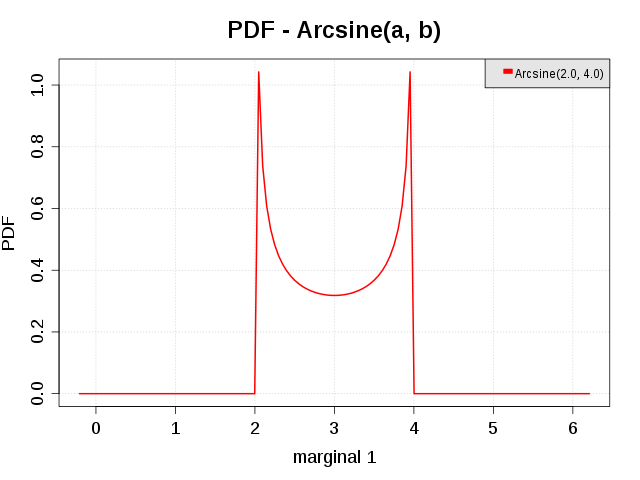
\includegraphics[width=7cm]{pdf_Arcsine.png}
      \caption{PDF of a Arcsine distribution.}
      \label{PDFArcsine}
    \end{center}
  \end{minipage}
  \hfill
  \begin{minipage}{10cm}
    \begin{center}
      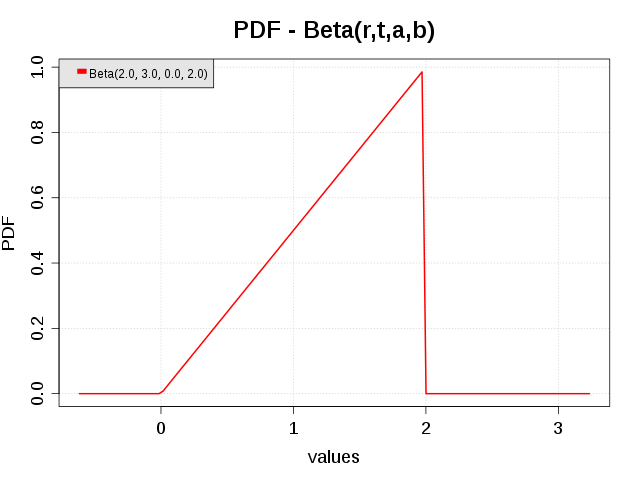
\includegraphics[width=7cm]{pdf_Beta_1.png}
      \caption{PDF of a Beta distribution.}
      \label{PDFBeta1}
    \end{center}
  \end{minipage}
\end{figure}

\begin{figure}[H]
  \begin{minipage}{10cm}
    \begin{center}
      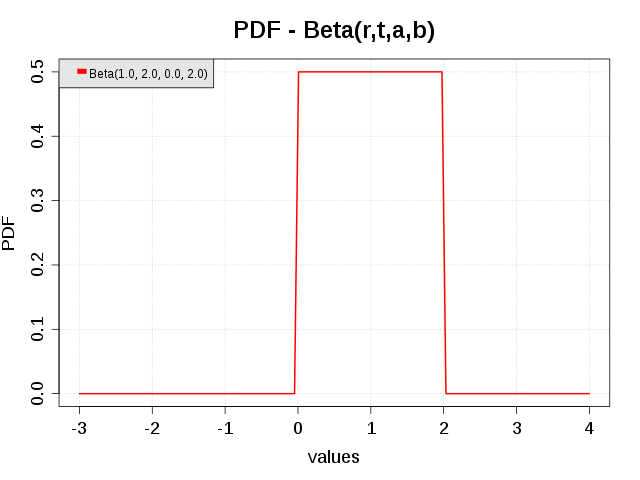
\includegraphics[width=7cm]{pdf_Beta_2.png}
      \caption{PDF of a Beta distribution.}
      \label{PDFBeta2}
    \end{center}
  \end{minipage}
  \hfill
  \begin{minipage}{10cm}
    \begin{center}
      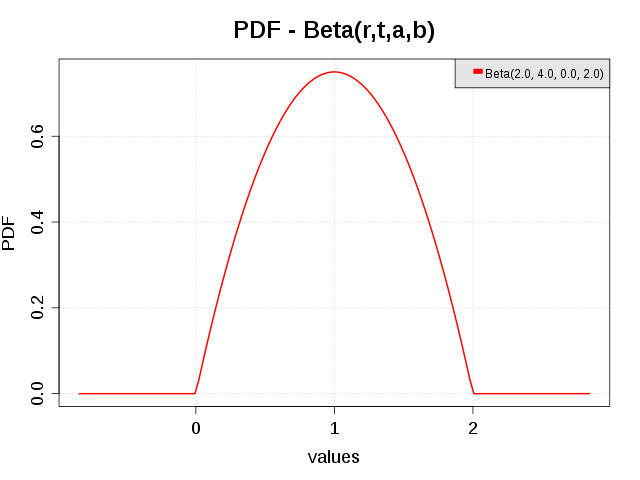
\includegraphics[width=7cm]{pdf_Beta_3.png}
      \caption{PDF of a Beta distribution.}
      \label{PDFBeta3}
    \end{center}
  \end{minipage}
\end{figure}

\begin{figure}[H]
  \begin{minipage}{10cm}
    \begin{center}
      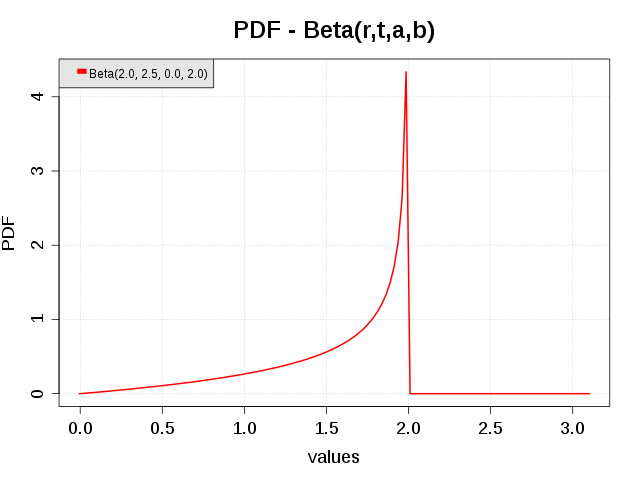
\includegraphics[width=7cm]{pdf_Beta_4.png}
      \caption{PDF of a Beta distribution.}
      \label{PDFBeta4}
    \end{center}
  \end{minipage}
  \hfill
  \begin{minipage}{10cm}
    \begin{center}
      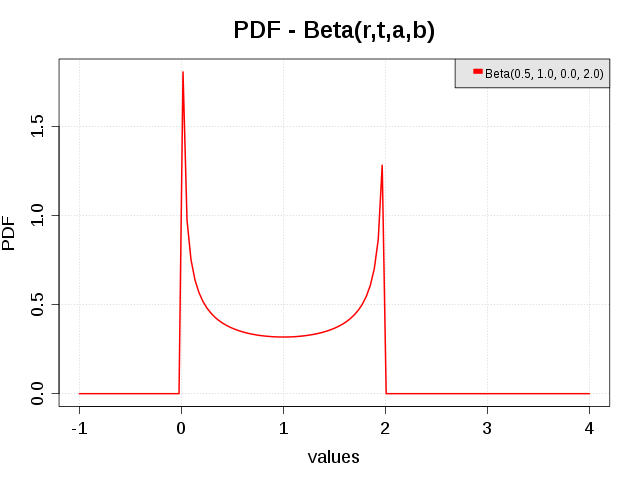
\includegraphics[width=7cm]{pdf_Beta_5.png}
      \caption{PDF of a Beta distribution.}
      \label{PDFBeta5}
    \end{center}
  \end{minipage}
\end{figure}


\begin{figure}[H]
  \begin{minipage}{10cm}
    \begin{center}
      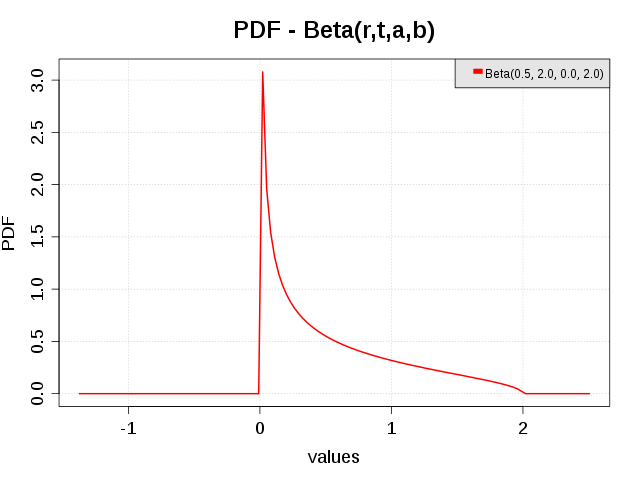
\includegraphics[width=7cm]{pdf_Beta_6.png}
      \caption{PDF of a Beta distribution.}
      \label{PDFBeta6}
    \end{center}
  \end{minipage}
  \hfill
  \begin{minipage}{10cm}
    \begin{center}
      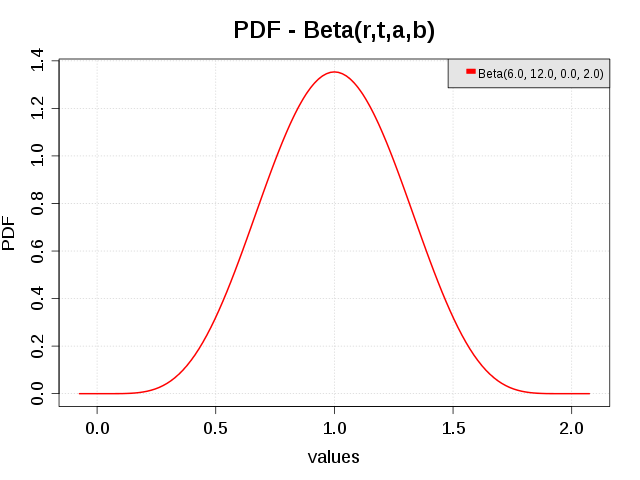
\includegraphics[width=7cm]{pdf_Beta_7.png}
      \caption{PDF of a Beta distribution.}
      \label{PDFBeta7}
    \end{center}
  \end{minipage}
\end{figure}


\begin{figure}[H]
  \begin{minipage}{10cm}
    \begin{center}
      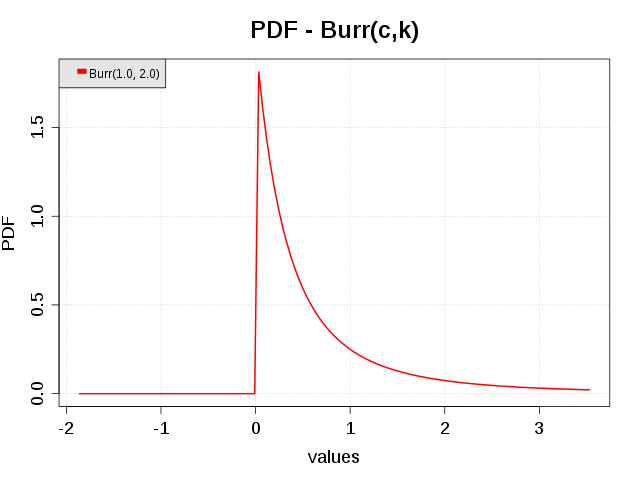
\includegraphics[width=7cm]{pdf_Burr_1.png}
      \caption{PDF of a Burr distribution.}
      \label{PDFBurr1}
    \end{center}
  \end{minipage}
  \hfill
  \begin{minipage}{10cm}
    \begin{center}
      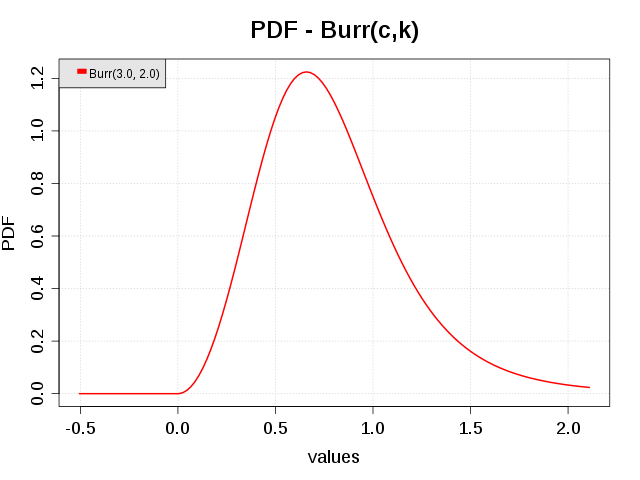
\includegraphics[width=7cm]{pdf_Burr_2.png}
      \caption{PDF of a Burr distribution.}
      \label{PDFBurr2}
    \end{center}
  \end{minipage}
\end{figure}


\begin{figure}[H]
  \begin{minipage}{10cm}
    \begin{center}
      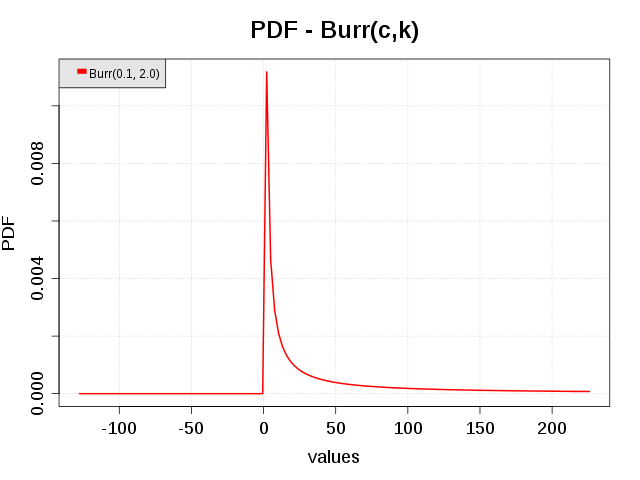
\includegraphics[width=7cm]{pdf_Burr_3.png}
      \caption{PDF of a Burr distribution.}
      \label{PDFBurr3}
    \end{center}
  \end{minipage}
  \hfill
  \begin{minipage}{10cm}
    \begin{center}
      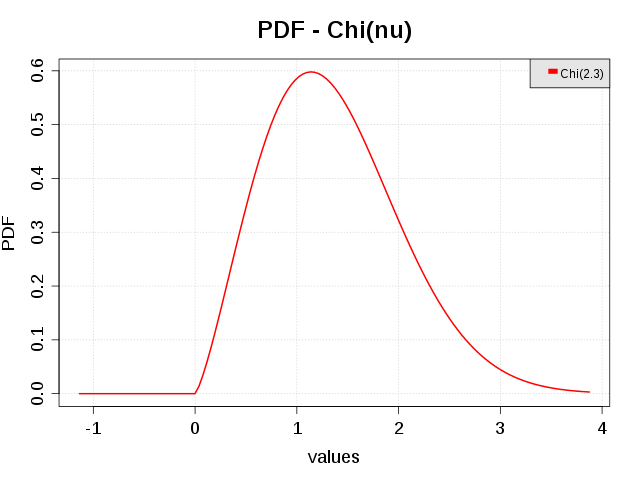
\includegraphics[width=7cm]{pdf_Chi_1.png}
      \caption{PDF of a Chi distribution.}
      \label{PDFChi1}
    \end{center}
  \end{minipage}
\end{figure}


\begin{figure}[H]
  \begin{minipage}{10cm}
    \begin{center}
      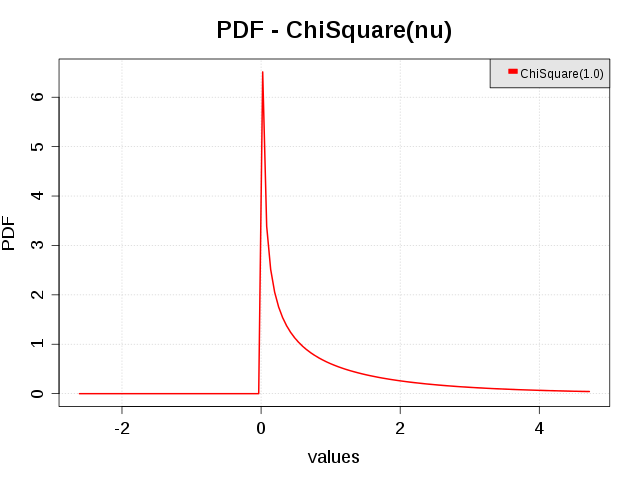
\includegraphics[width=7cm]{pdf_ChiSquare_1}
      \caption{PDF of a Chi Square distribution.}
      \label{PDFChiSquare1}
    \end{center}
  \end{minipage}
  \hfill
  \begin{minipage}{10cm}
    \begin{center}
      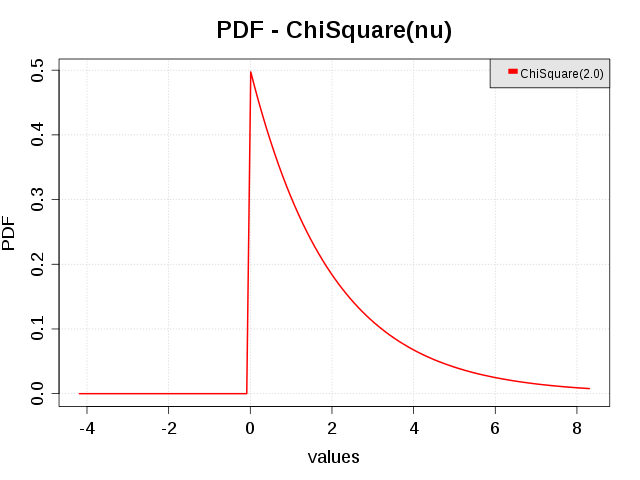
\includegraphics[width=7cm]{pdf_ChiSquare_2.png}
      \caption{PDF of a Chi Square distribution.}
      \label{PDFChiSquare2}
    \end{center}
  \end{minipage}
\end{figure}


\begin{figure}[H]
  \begin{minipage}{10cm}
    \begin{center}
      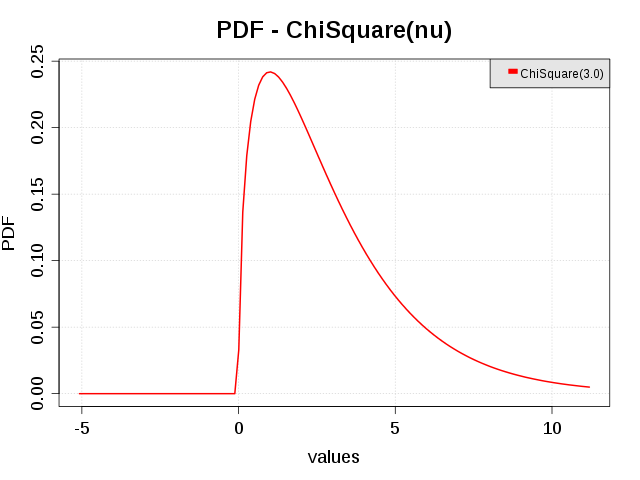
\includegraphics[width=7cm]{pdf_ChiSquare_3.png}
      \caption{PDF of a Chi Square distribution.}
      \label{PDFChiSquare3}
    \end{center}
  \end{minipage}
  \hfill
  \begin{minipage}{10cm}
    \begin{center}
      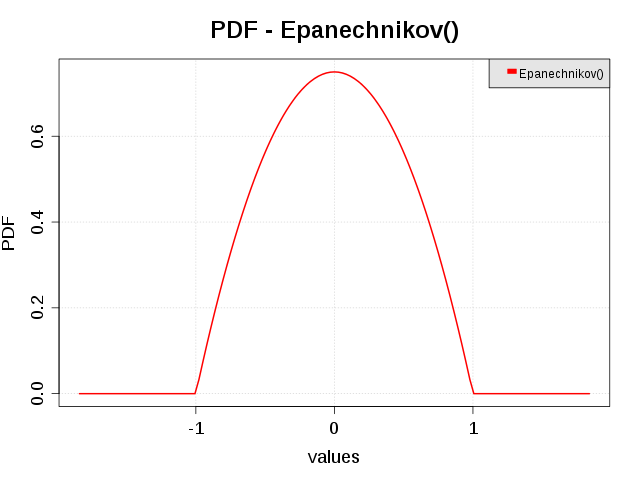
\includegraphics[width=7cm]{pdf_Epanechnikov.png}
      \caption{PDF of an Epanechnikov distribution.}
      \label{PDFEpanechnikov}
    \end{center}
  \end{minipage}
\end{figure}


\begin{figure}[H]
  \begin{minipage}{10cm}
    \begin{center}
      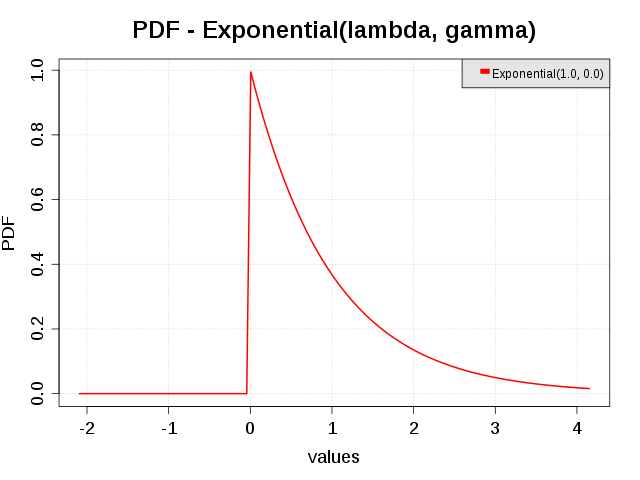
\includegraphics[width=7cm]{pdf_Exponential.png}
      \caption{PDF of a Exponential distribution.}
      \label{PDFExponential}
    \end{center}
  \end{minipage}
  \hfill
  \begin{minipage}{10cm}
    \begin{center}
      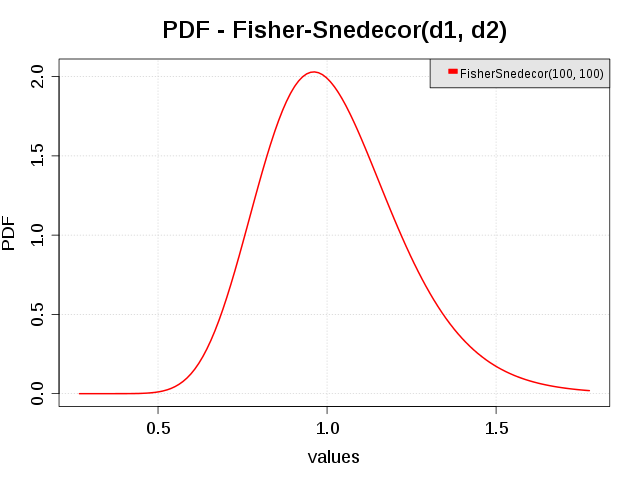
\includegraphics[width=7cm]{pdf_FisherSnedecor_1.png}
      \caption{PDF of a Fisher-Snedecor distribution.}
      \label{PDFFisherSnedecor1}
    \end{center}
  \end{minipage}
\end{figure}



\begin{figure}[H]
  \begin{minipage}{10cm}
    \begin{center}
      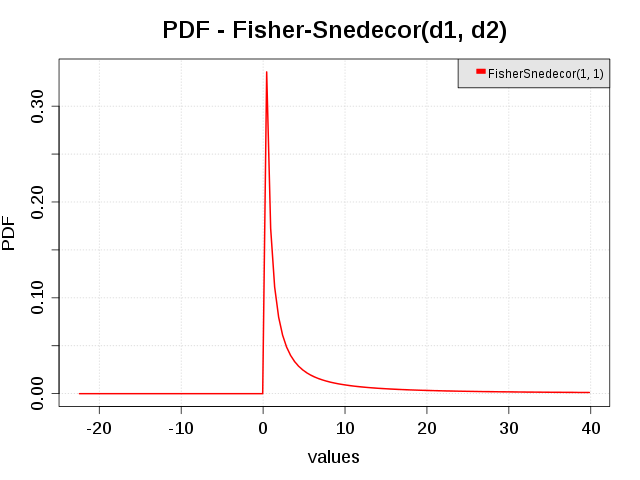
\includegraphics[width=7cm]{pdf_FisherSnedecor_2.png}
      \caption{PDF of a Fisher-Snedecor distribution.}
      \label{PDFFisherSnedecor2}
    \end{center}
  \end{minipage}
  \hfill
  \begin{minipage}{10cm}
    \begin{center}
      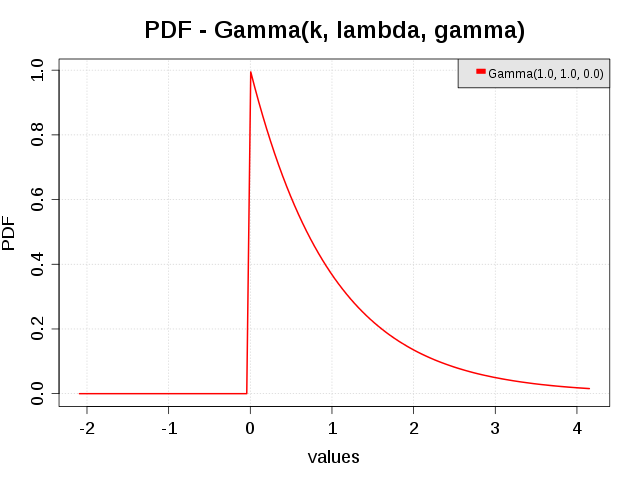
\includegraphics[width=7cm]{pdf_Gamma_1.png}
      \caption{PDF of a Gamma distribution.}
      \label{PDFGamma1}
    \end{center}
  \end{minipage}
\end{figure}

\begin{figure}[H]
  \begin{minipage}{10cm}
    \begin{center}
      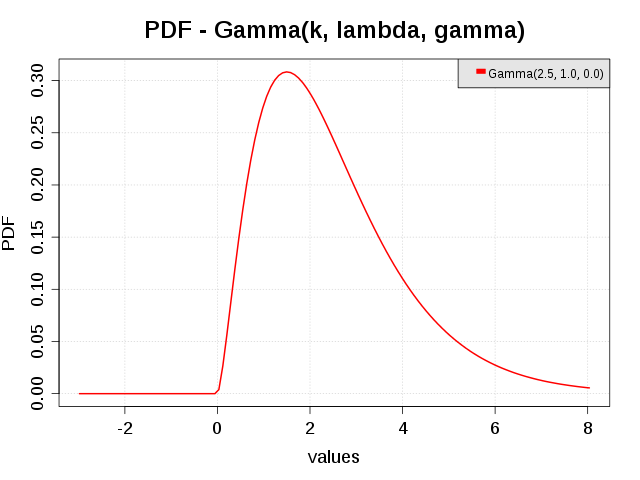
\includegraphics[width=7cm]{pdf_Gamma_2.png}
      \caption{PDF of a Gamma distribution.}
      \label{PDFGamma2}
    \end{center}
  \end{minipage}
  \hfill
  \begin{minipage}{10cm}
    \begin{center}
      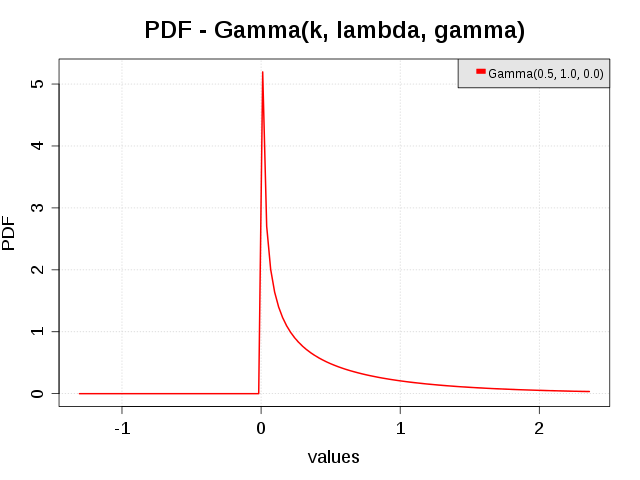
\includegraphics[width=7cm]{pdf_Gamma_3.png}
      \caption{PDF of a Gamma distribution.}
      \label{PDFGamma3}
    \end{center}
  \end{minipage}
\end{figure}




\begin{figure}[H]
  \begin{minipage}{10cm}
    \begin{center}
      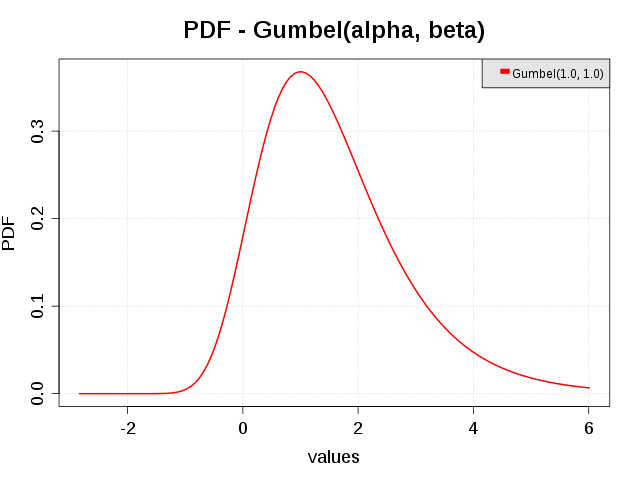
\includegraphics[width=7cm]{pdf_Gumbel.png}
      \caption{PDF of a Gumbel distribution.}
      \label{PDFGumbel}
    \end{center}
  \end{minipage}
  \hfill
  \begin{minipage}{10cm}
    \begin{center}
      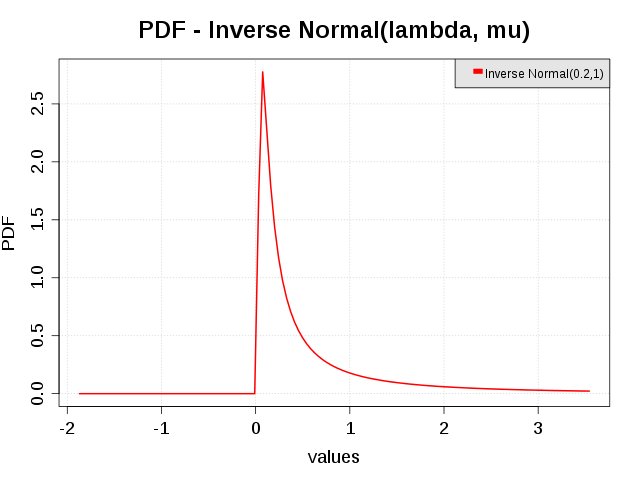
\includegraphics[width=7cm]{pdf_InverseNormal_1.png}
      \caption{PDF of a InverseNormal distribution.}
      \label{PDFInverseNormal1}
    \end{center}
  \end{minipage}
\end{figure}




\begin{figure}[H]
  \begin{minipage}{10cm}
    \begin{center}
      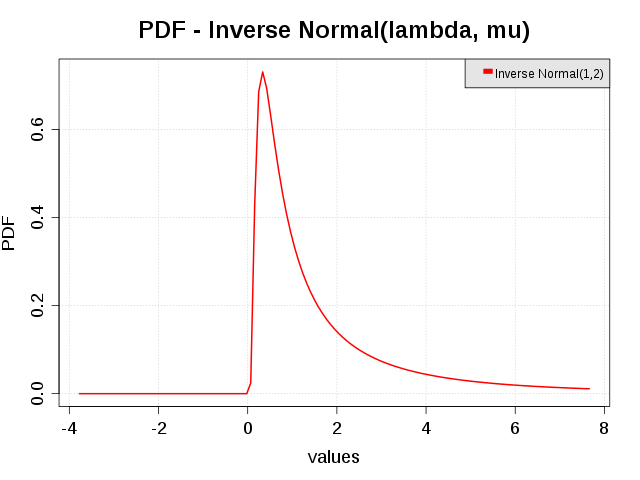
\includegraphics[width=7cm]{pdf_InverseNormal_2.png}
      \caption{PDF of a InverseNormal distribution.}
      \label{PDFInverseNormal2}
    \end{center}
  \end{minipage}
  \hfill
  \begin{minipage}{10cm}
    \begin{center}
      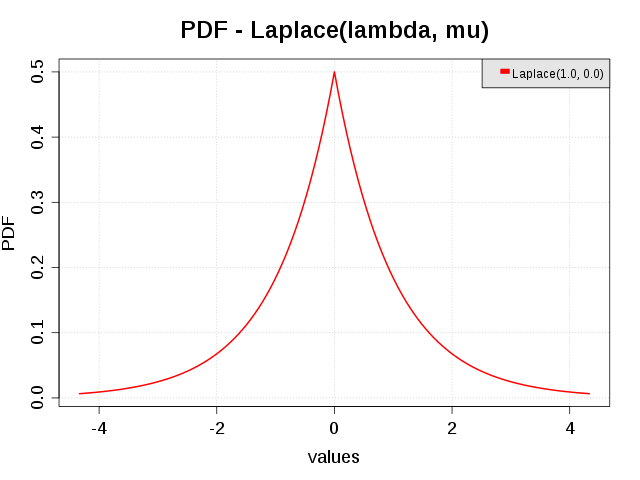
\includegraphics[width=7cm]{pdf_Laplace.png}
      \caption{PDF of a Laplace distribution.}
      \label{PDFLaplace}
    \end{center}
  \end{minipage}
\end{figure}




\begin{figure}[H]
  \begin{minipage}{10cm}
    \begin{center}
      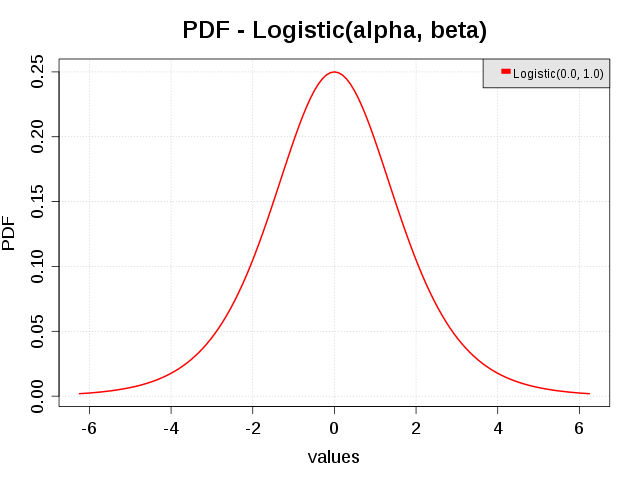
\includegraphics[width=7cm]{pdf_Logistic.png}
      \caption{PDF of a Logistic distribution.}
      \label{PDFLogistic}
    \end{center}
  \end{minipage}
  \hfill
  \begin{minipage}{10cm}
    \begin{center}
      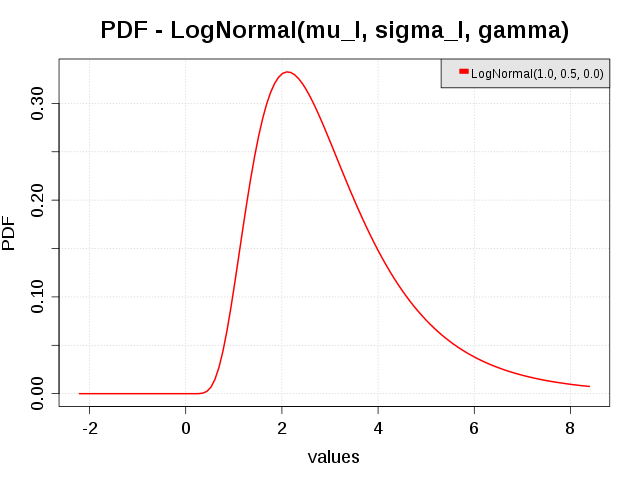
\includegraphics[width=7cm]{pdf_LogNormal.png}
      \caption{PDF of a  LogNormal distribution.}
      \label{PDFLogNormal}
    \end{center}
  \end{minipage}
\end{figure}






\begin{figure}[H]
  \begin{minipage}{10cm}
    \begin{center}
      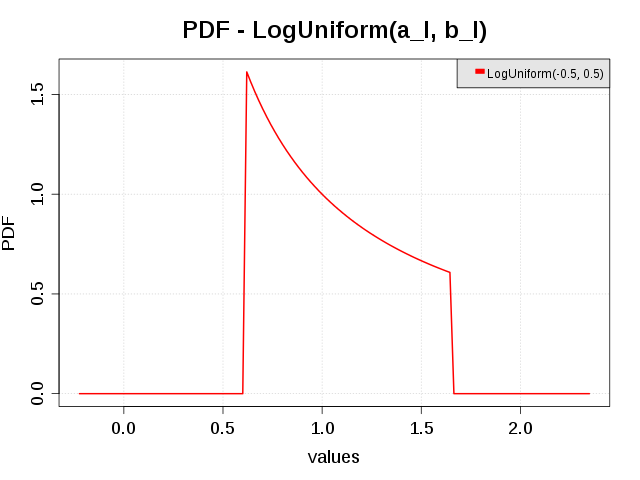
\includegraphics[width=7cm]{pdf_LogUniform.png}
      \caption{PDF of a  LogUniform distribution.}
      \label{PDFLogUniform}
    \end{center}
  \end{minipage}
  \hfill
  \begin{minipage}{10cm}
    \begin{center}
      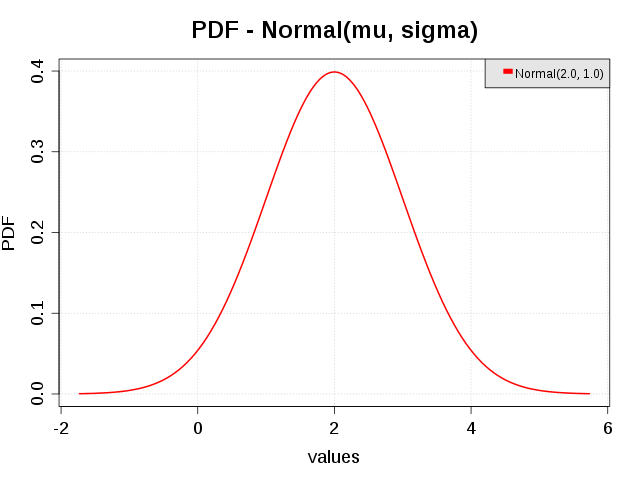
\includegraphics[width=7cm]{pdf_Normal.png}
      \caption{PDF of a Normal distribution.}
      \label{PDFNormal}
    \end{center}
  \end{minipage}
\end{figure}



\begin{figure}[H]
  \begin{minipage}{10cm}
    \begin{center}
      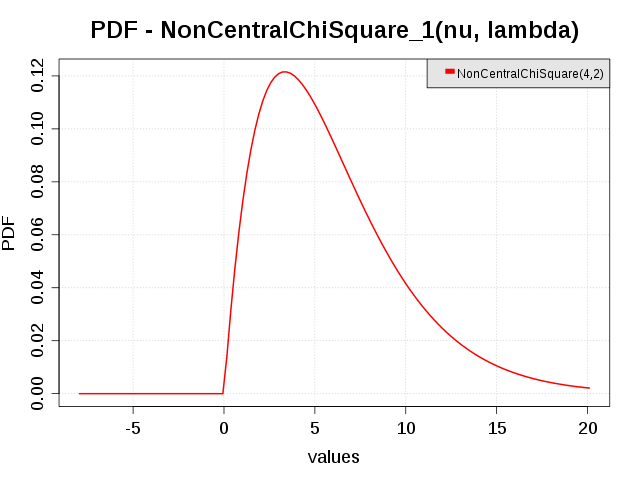
\includegraphics[width=7cm]{pdf_NonCentralChiSquare_1.png}
      \caption{PDF of a Non Central Chi Square distribution.}
      \label{PDFNonCentralChiSquare1}
    \end{center}
  \end{minipage}
  \hfill
  \begin{minipage}{10cm}
    \begin{center}
      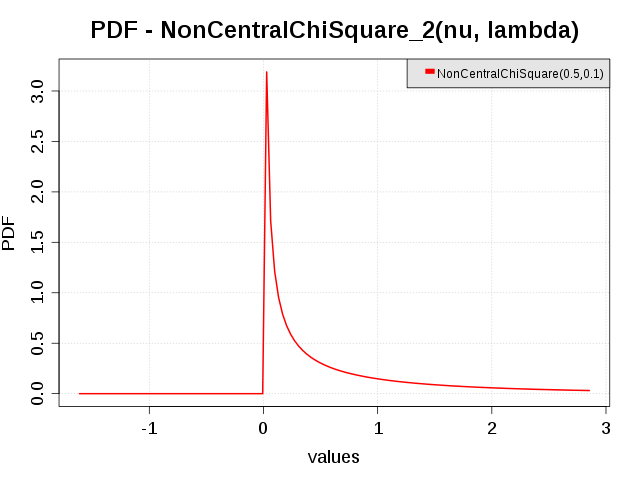
\includegraphics[width=7cm]{pdf_NonCentralChiSquare_2.png}
      \caption{PDF of a Non Central Chi Square distribution.}
      \label{PDFNonCentralChiSquare2}
    \end{center}
  \end{minipage}
\end{figure}


\begin{figure}[H]
  \begin{minipage}{10cm}
    \begin{center}
      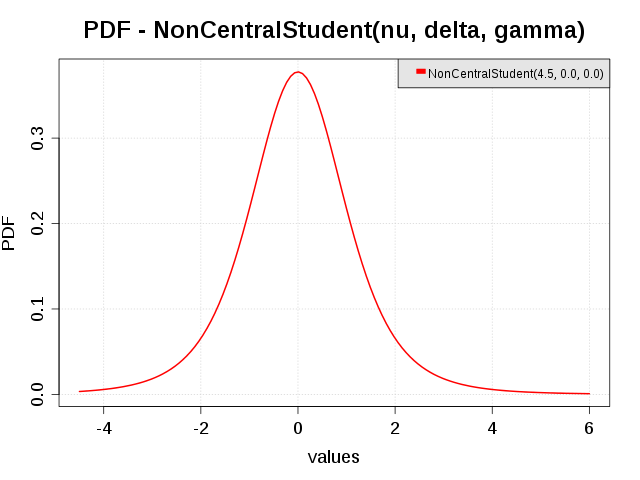
\includegraphics[width=7cm]{pdf_NonCentralStudent.png}
      \caption{PDF of a Non Central Student distribution.}
      \label{PDFNonCentralStudent}
    \end{center}
  \end{minipage}
  \hfill
  \begin{minipage}{10cm}
    \begin{center}
      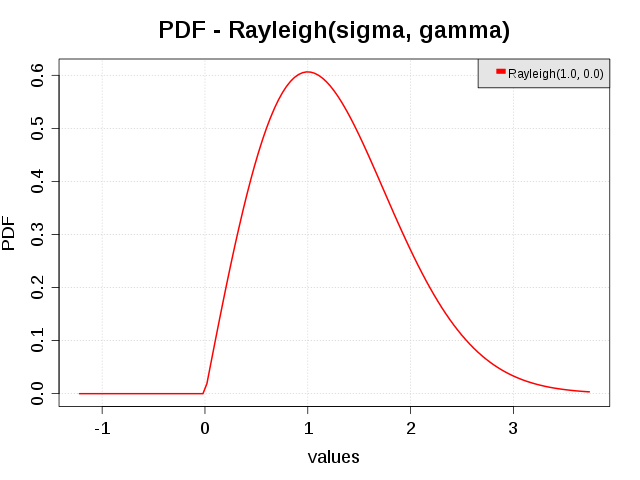
\includegraphics[width=7cm]{pdf_Rayleigh.png}
      \caption{PDF of a Rayleigh distribution.}
      \label{PDFRayleigh}
    \end{center}
  \end{minipage}
\end{figure}


\begin{figure}[H]
  \begin{minipage}{10cm}
    \begin{center}
      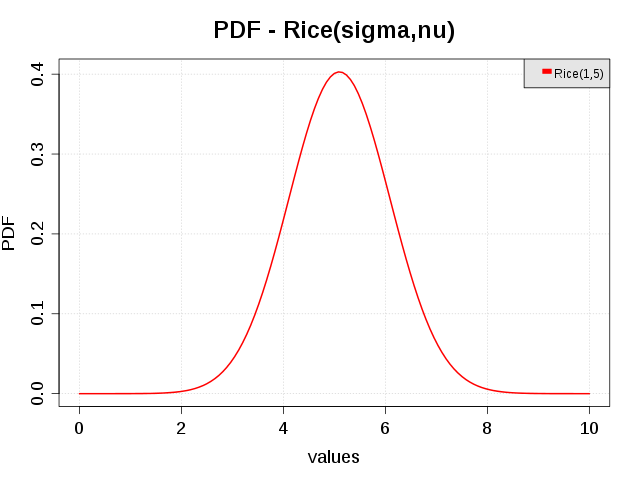
\includegraphics[width=7cm]{pdf_Rice_1.png}
      \caption{PDF of a Rice distribution.}
      \label{PDFRice1}
    \end{center}
  \end{minipage}
  \hfill
  \begin{minipage}{10cm}
    \begin{center}
      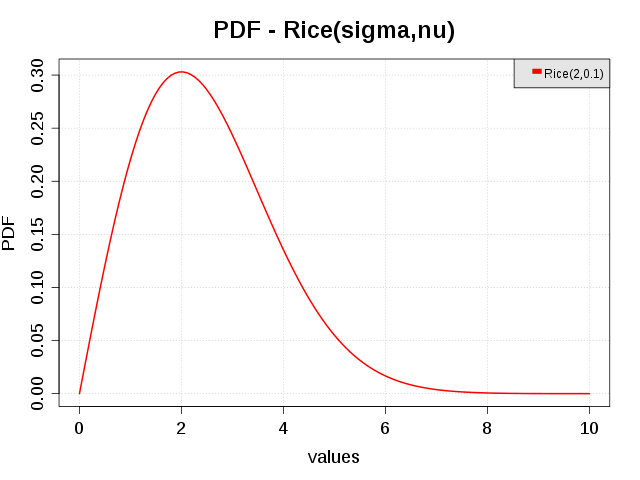
\includegraphics[width=7cm]{pdf_Rice_2.png}
      \caption{PDF of a Rice distribution.}
      \label{PDFRice2}
    \end{center}
  \end{minipage}
\end{figure}


\begin{figure}[H]
  \begin{minipage}{10cm}
    \begin{center}
      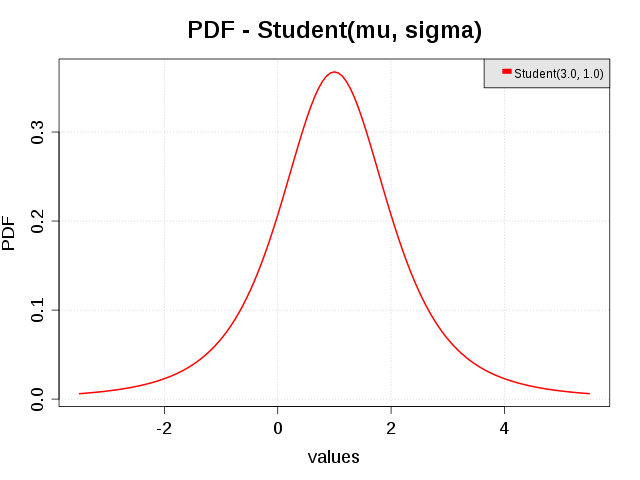
\includegraphics[width=7cm]{pdf_Student.png}
      \caption{PDF of a Student distribution.}
      \label{PDFStudent}
    \end{center}
  \end{minipage}
  \hfill
  \begin{minipage}{10cm}
    \begin{center}
      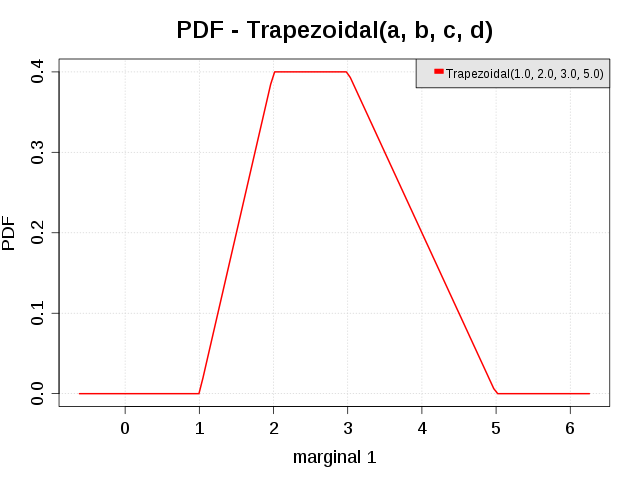
\includegraphics[width=7cm]{pdf_Trapezoidal.png}
      \caption{PDF of a Trapezoidal distribution.}
      \label{PDFTrapezoidal}
    \end{center}
  \end{minipage}
\end{figure}

\begin{figure}[H]
  \begin{minipage}{10cm}
    \begin{center}
      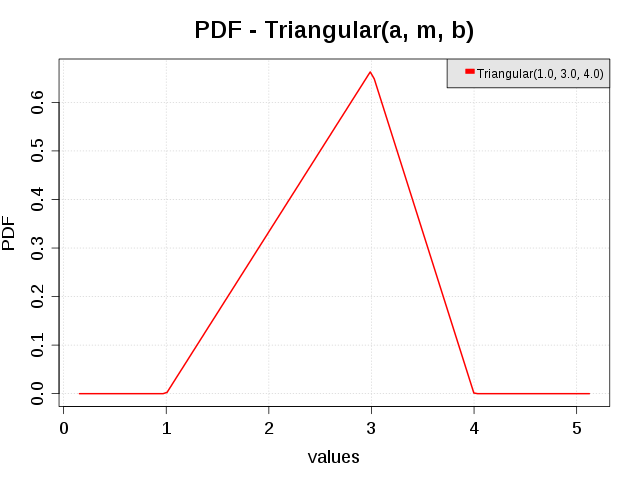
\includegraphics[width=7cm]{pdf_Triangular.png}
      \caption{PDF of a  Triangular distribution.}
      \label{PDFTriangular}
    \end{center}
  \end{minipage}
  \hfill
  \begin{minipage}{10cm}
    \begin{center}
      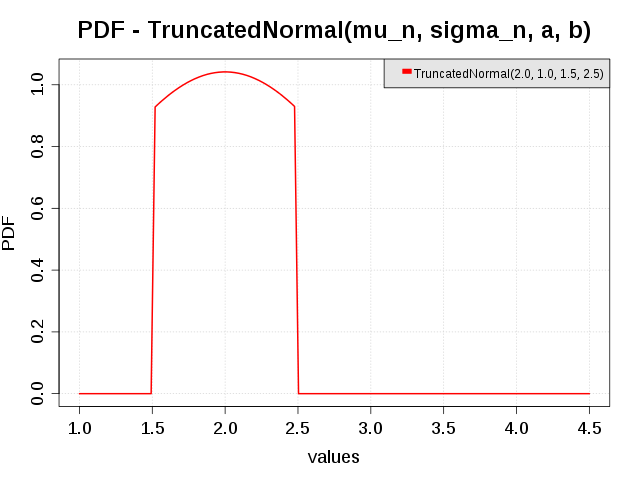
\includegraphics[width=7cm]{pdf_TruncatedNormal_1.png}
      \caption{PDF of a  Truncated Normal distribution.}
      \label{PDFTruncatedNormal1}
    \end{center}
  \end{minipage}
\end{figure}

\begin{figure}[H]
  \begin{minipage}{10cm}
    \begin{center}
      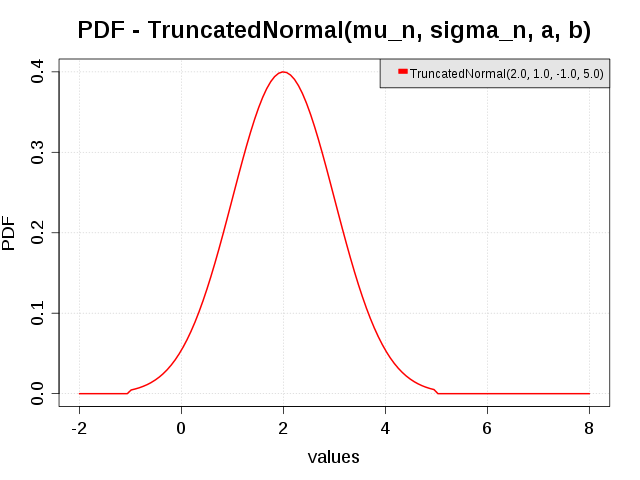
\includegraphics[width=7cm]{pdf_TruncatedNormal_2.png}
      \caption{PDF of a  Truncated Normal distribution.}
      \label{PDFTruncatedNormal2}
    \end{center}
  \end{minipage}
  \hfill
  \begin{minipage}{10cm}
    \begin{center}
      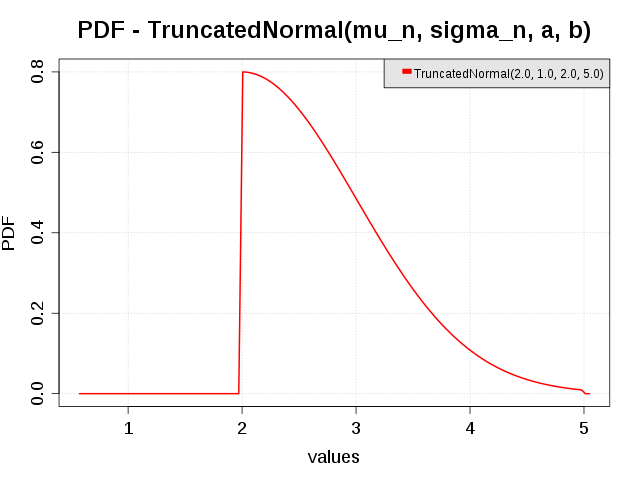
\includegraphics[width=7cm]{pdf_TruncatedNormal_3.png}
      \caption{PDF of a  Truncated Normal distribution.}
      \label{PDFTruncatedNormal3}
    \end{center}
  \end{minipage}
\end{figure}

\begin{figure}[H]
  \begin{minipage}{10cm}
    \begin{center}
      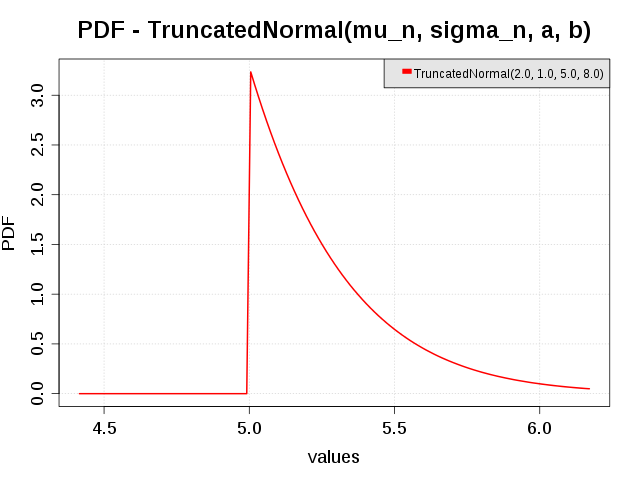
\includegraphics[width=7cm]{pdf_TruncatedNormal_4.png}
      \caption{PDF of a  TruncatedNormaldistribution.}
      \label{PDFTruncatedNormal4}
    \end{center}
  \end{minipage}
  \hfill
  \begin{minipage}{10cm}
    \begin{center}
      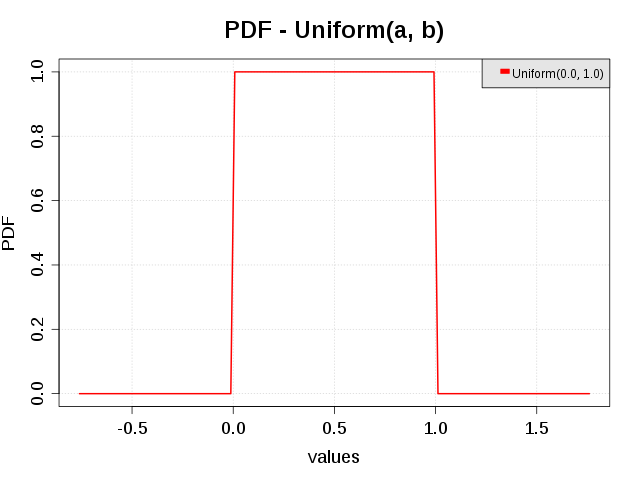
\includegraphics[width=7cm]{pdf_Uniform.png}
      \caption{PDF of a  Uniform distribution.}
      \label{PDFUniform}
    \end{center}
  \end{minipage}
\end{figure}




\begin{figure}[H]
  \begin{minipage}{10cm}
    \begin{center}
      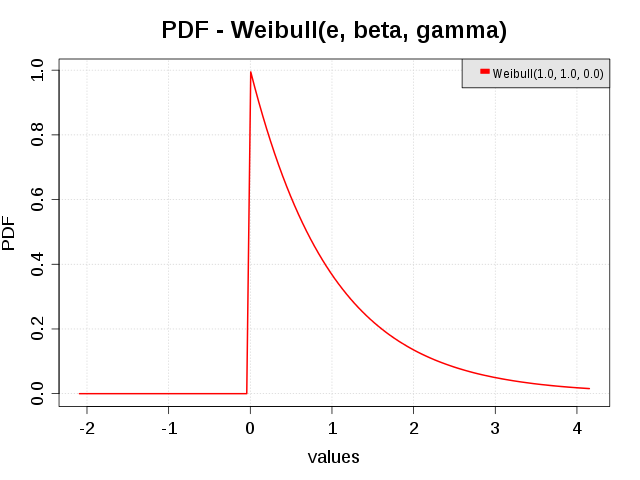
\includegraphics[width=7cm]{pdf_Weibull_1.png}
      \caption{PDF of a  Weibull distribution.}
      \label{PDFWeibull1}
    \end{center}
  \end{minipage}
  \hfill
  \begin{minipage}{10cm}
    \begin{center}
      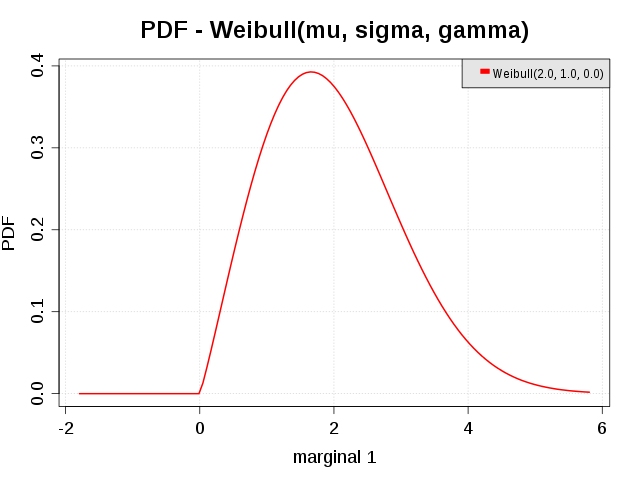
\includegraphics[width=7cm]{pdf_Weibull_2.png}
      \caption{PDF of a Weibull distribution.}
      \label{PDFWeibull2}
    \end{center}
  \end{minipage}
\end{figure}





The Histogram distribution explicited in the Use Case is drawn in Figures \ref{PDFHistogram} and \ref{CDFHistogram}.

\begin{figure}[H]
  \begin{minipage}{10cm}
    \begin{center}
      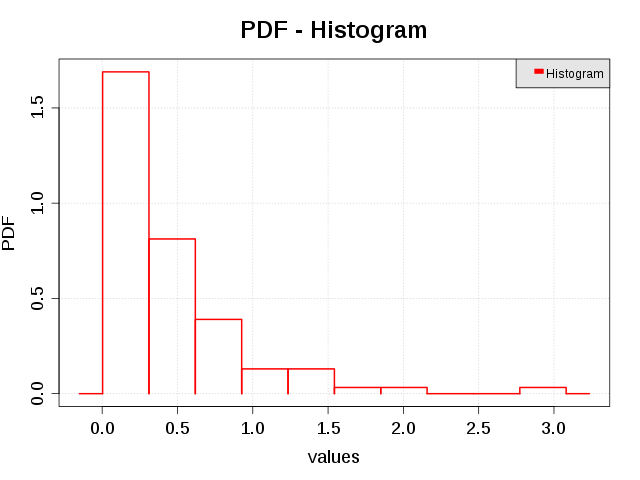
\includegraphics[width=7cm]{pdf_Histogram.png}
      \caption{PDF of an Histogram distribution.}
      \label{PDFHistogram}
    \end{center}
  \end{minipage}
  \hfill
  \begin{minipage}{10cm}
    \begin{center}
      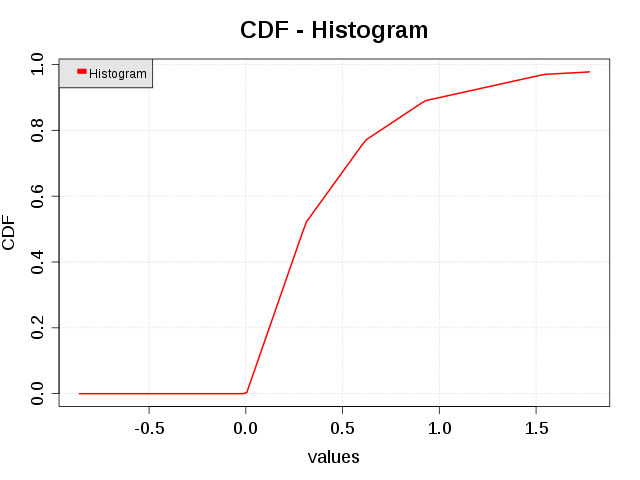
\includegraphics[width=7cm]{cdf_Histogram.png}
      \caption{CDF of an Histogram distribution.}
      \label{CDFHistogram}
    \end{center}
  \end{minipage}
\end{figure}




The discrete distributions explicited in the Use Case  have the following distribution graphs, drawn in Figures \ref{PDFBernoulli} to Figure \ref{CDFUserDefined}.



\begin{figure}[H]
  \begin{minipage}{10cm}
    \begin{center}
      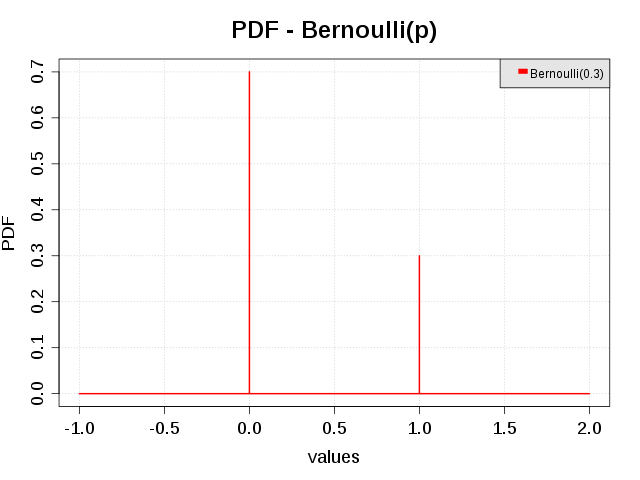
\includegraphics[width=7cm]{pdf_Bernoulli.png}
      \caption{Distribution of a Bernoulli distribution.}
      \label{PDFBernoulli}
    \end{center}
  \end{minipage}
  \hfill
  \begin{minipage}{10cm}
    \begin{center}
      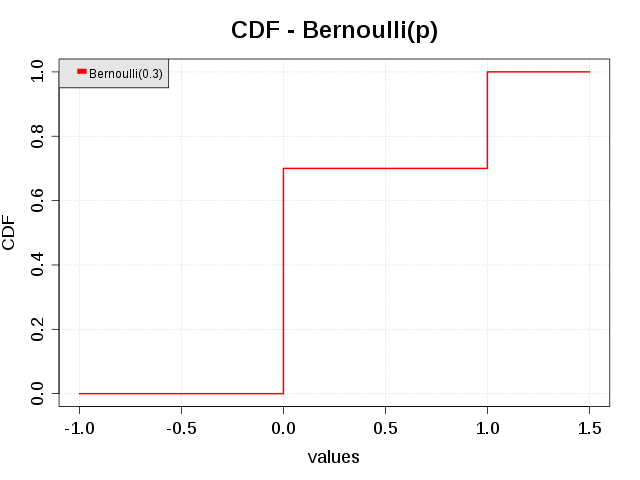
\includegraphics[width=7cm]{cdf_Bernoulli.png}
      \caption{CDF of a Bernoulli distribution.}
      \label{CDFBernoulli}
    \end{center}
  \end{minipage}
\end{figure}





\begin{figure}[H]
  \begin{minipage}{10cm}
    \begin{center}
      \includegraphics[width=7cm]{pdf_Binomial.png}
      \caption{Distribution of a Binomial distribution.}
      \label{PDFBinomial}
    \end{center}
  \end{minipage}
  \hfill
  \begin{minipage}{10cm}
    \begin{center}
      \includegraphics[width=7cm]{cdf_Binomial.png}
      \caption{CDF of a Binomial distribution.}
      \label{CDFBinomial}
    \end{center}
  \end{minipage}
\end{figure}



\begin{figure}[H]
  \begin{minipage}{10cm}
    \begin{center}
      \includegraphics[width=7cm]{pdf_Geometric.png}
      \caption{Distribution of a Geometric distribution.}
      \label{PDFGeometric}
    \end{center}
  \end{minipage}
  \hfill
  \begin{minipage}{10cm}
    \begin{center}
      \includegraphics[width=7cm]{cdf_Geometric.png}
      \caption{CDF of a Geometric distribution.}
      \label{CDFGeometric}
    \end{center}
  \end{minipage}
\end{figure}



\begin{figure}[H]
  \begin{minipage}{10cm}
    \begin{center}
      \includegraphics[width=7cm]{pdf_Poisson.png}
      \caption{Distribution of a Poisson distribution.}
      \label{PDFPoisson}
    \end{center}
  \end{minipage}
  \hfill
  \begin{minipage}{10cm}
    \begin{center}
      \includegraphics[width=7cm]{cdf_Poisson.png}
      \caption{CDF of a Poisson distribution.}
      \label{CDFPoisson}
    \end{center}
  \end{minipage}
\end{figure}



\begin{figure}[H]
  \begin{minipage}{10cm}
    \begin{center}
      \includegraphics[width=7cm]{pdf_UserDefined.png}
      \caption{Distribution of a  UserDefined distribution.}
      \label{PDFUserDefined}
    \end{center}
  \end{minipage}
  \hfill
  \begin{minipage}{10cm}
    \begin{center}
      \includegraphics[width=7cm]{cdf_UserDefined.png}
      \caption{CDF of a UserDefined distribution.}
      \label{CDFUserDefined}
    \end{center}
  \end{minipage}
\end{figure}



\begin{figure}[H]
  \begin{minipage}{10cm}
    \begin{center}
      \includegraphics[width=7cm]{pdf_ZipfMandelbrot_1.png}
      \caption{Distribution of a  Zipf-Mandelbrot distribution.}
      \label{PDFZipfMandelbrot}
    \end{center}
  \end{minipage}
  \hfill
  \begin{minipage}{10cm}
    \begin{center}
      \includegraphics[width=7cm]{cdf_ZipfMandelbrot_1.png}
      \caption{CDF of a Zipf-Mandelbrot  distribution.}
      \label{CDFZipfMandelbrot}
    \end{center}
  \end{minipage}
\end{figure}


\newpage % Copyright (c)  2005-2010 EDF-EADS-PHIMECA.
% Permission is granted to copy, distribute and/or modify this document
% under the terms of the GNU Free Documentation License, Version 1.2
% or any later version published by the Free Software Foundation;
% with no Invariant Sections, no Front-Cover Texts, and no Back-Cover
% Texts.  A copy of the license is included in the section entitled "GNU
% Free Documentation License".
\renewcommand{\filename}{docUC_InputNoData_TruncatedDist.tex}
\renewcommand{\filetitle}{UC : Creation of a truncated distribution}

% \HeaderNNIILevel
% \HeaderIILevel
\HeaderIIILevel
\label{truncatedistribution}




\index{Usual Distribution!Truncated distribution}

The objective of the Use Case is to truncate a 1D distribution already defined. Open TURNS enables to truncate the distribution in its lower area, or its upper area or in both lower and upper areas. After having  truncated a distribution, it is possible to recuperate the initial distribution thanks to the method {\itshape getDistribution()}.\\

Details on each object may be found in the User Manual  (\href{OpenTURNS_UserManual_TUI.pdf}{see User Manual - Probabilistic modeling / Truncated Distributions}).\\

Let's consider $X$ a random variable with respectively $F_X$ and $p_X$ its cumulative and probability density functions, and $(a,b)\in \mathbb{R} \cup {\pm \infty}$. The random variable $Y=X/[a,b]$ which is the random variable $X$ given that $X\in[a,b]$ is defined by the following cumulative and probability density functions $F_Y$ and $p_Y$ :
$$
\forall y \in \mathbb{R}, F_Y(y) = Prob(X<y\, / \, X\in[a,b]) =
\begin{array}{|ll}
  1 & \mbox{for } y \geq b, \\
  0 & \mbox{for } y \leq a, \\
  \displaystyle \frac{F_X(y) - F_X(a)}{F_X(b) - F_X(a)} & \mbox{for } y\in[a,b]
\end{array}
$$
$$
\forall y \in \mathbb{R}, p_Y(y) =
\begin{array}{|ll}
  0 &  \mbox{for } y \geq b  \mbox{ or }  y \leq a\\
  \displaystyle \frac{1}{F_X(b) - F_X(a)}\, p_X(y) & \mbox{for } y\in[a,b]
\end{array}
$$





\noindent%
\requirements{
  \begin{description}
  \item[$\bullet$] some lower and upper bounds : {\itshape myLowerBound, myUpperBound}
  \item[type:] reals
  \item[$\bullet$] a 1D distribution : {\itshape myEntireDistribution}
  \item[type:] a Distribution which implementation is UsualDistribution or ComposedDistribution or Mixture
  \end{description}
}
{
  \begin{description}
  \item[$\bullet$] a distribution : {\itshape myTruncatedDistribution}
  \item[type:]  a TruncatedDistribution
  \end{description}
}

\textspace\\
Python script for this UseCase :

\begin{lstlisting}

  # CASE 1 : Truncate the distribution within the range $[myLowerBound, myUpperBound]$
  myTruncatedDistribution = TruncatedDistribution(myEntireDistribution, myLowerBound, myUpperBound)


  # CASE 2 : Truncate the distribution within the range $[myLowerBound, \infty[$ or $[myLowerBound, max[$ if
  # myEntireDistribution was already bounded by $max$
  myTruncatedDistribution = TruncatedDistribution(myEntireDistribution, myLowerBound, TruncatedDistribution.LOWER)


  # CASE 3 : Truncate the distribution within the range $[-\infty, myUpperBound[$ or $[min, myUpperBound[$ if
  # myEntireDistribution was already bounded by $min$
  myTruncatedDistribution = TruncatedDistribution(myEntireDistribution, myUpperBound, TruncatedDistribution.UPPER)

  # Recuperate the initial distribution
  initialDistribution = myTruncatedDistribution.getDistribution()
\end{lstlisting}

\textspace\\

Figures \ref{truncatedDistribution_pdf} and \ref{truncatedDistribution_cdf} show the PDF and CDF of the truncated distributions of a Logistic($\alpha = 1.0$, $\beta  =2.0$) respectively within the ranges $[4.0, \infty[$,  $[-2.0, 5.0]$ and $[-\infty, 3.0]$.

\begin{figure}[H]
  \begin{center}
    \includegraphics[width=10cm]{truncatedDistribution_pdf.png}
  \end{center}
  \caption{PDF of several truncated Logistic distributions}
  \label{truncatedDistribution_pdf}
\end{figure}

\begin{figure}[H]
  \begin{center}
    \includegraphics[width=10cm]{truncatedDistribution_cdf.png}
  \end{center}
  \caption{CDF of several truncated Logistic distributions}
  \label{truncatedDistribution_cdf}
\end{figure}


\newpage % Copyright (c)  2005-2010 EDF-EADS-PHIMECA.
% Permission is granted to copy, distribute and/or modify this document
% under the terms of the GNU Free Documentation License, Version 1.2
% or any later version published by the Free Software Foundation;
% with no Invariant Sections, no Front-Cover Texts, and no Back-Cover
% Texts.  A copy of the license is included in the section entitled "GNU
% Free Documentation License".
\renewcommand{\filename}{docUC_InputNoData_Copula}
\renewcommand{\filetitle}{UC : Creation of a copula and a composed copula}

% \HeaderNNIILevel
% \HeaderIILevel
\HeaderIIILevel








The objective of this Use Case is to manipulate copulas of Open TURNS.\\

A copula may be considered as the restriction to $[0,1]^n$ of a distribution with uniform 1D marginals on $[0,1]$ and this copula as copula. That's why an object of type {\itshape Copula} offers the same methods as an object of type {\itshape Distribution} (see U.C. \ref{manipulation_distribution} to have the list of the methods).\\

Details on copula may be found in the Reference Guide (\href{OpenTURNS_ReferenceGuide.pdf}{see file Reference Guide - Step B -- Copula}).\\

Details on each object may be found in the User Manual  (\href{OpenTURNS_UserManual_TUI.pdf}{see User Manual - Probabilistic modeling / Composed Distributions}).\\


\index{Copula!Composed copula}
\index{Copula!Clayton}
\index{Copula!Gumbel}
\index{Copula!Frank}
\index{Copula!Normal}
\index{Copula!Independent}
\index{Correlation!Correlation matrix of the Normal copula}
\index{Correlation!Spearman rank correlation matrix}


Open TURNS proposes some bidimensional copulas, listed in Table. \ref{ListCopulas}. One is elliptical : Normal copula, the others are archimedean : Frank, Clayton, Gumbel. The Independent one is both elliptical and archimedean.\\


Furthermore, Open TURNS is able to extract the copula $C$ from any $n$ dimensional distribution, thanks to the inverse of the Sklar theorem :
$$
C(u_1, \dots, u_n) = F(F_1^{-1}(u_1), \dots, F_n^{-1}(u_n))
$$
where $F$ is the cumulative density function of the distribution and $F_i$ its respective marginals. This copula is denoted \emph{Sklar Copula} within Open TURNS.\\


\newcommand\B{\rule[-2.4ex]{0pt}{0pt}}

\begin{table}[H]
  \begin{center}
    \begin{tabular}{|l|c|c|c|}
      \hline
      Name & Dimension & $C(u_1, \cdots, u_n)$ & Parameters\textspace\B\\
      \hline
      Independent & n& $\displaystyle \prod_{i=1}^{i=n} u_i$ & n \textspace\B\\
      \hline
      Normal & 2 &  $\displaystyle\int_{-\infty}^{\Phi^{-1}(u_1)}\int_{-\infty}^{\Phi^{-1}(u_2)}\frac{1}{2\pi\sqrt{1-\rho^2}}\exp\left(-\frac{s^2-2\rho st+t^2}{2(1-\rho^2)}\right)\,\Diff s\,\Diff t$ \mathspace\B & $\begin{array}{l}
        \mat{R} = \left(\begin{array}{cc}
            1 & \rho \\
            \rho & 1
          \end{array}
        \right)\\
        \rho \in [-1,1]
      \end{array}$\\
      \hline
      Normal & n & $\displaystyle\int_{-\infty}^{\Phi^{-1}(u_1)}\cdots \int_{-\infty}^{\Phi^{-1}(u_n)}\frac{1}{(2\pi)^{n/2} \sqrt{\det(\mat{R})}}\exp\left(-\frac{1}{2}\vect{x}^t \mat{R}^{-1} \vect{x} \right)\,\Diff \vect{x}$ & $\mat{R}$, SDP \textspace\B\\
      \hline
      % Student & 2 & $\displaystyle\int_{-\infty}^{T_{\nu}^{-1}(u_1)}\int_{-\infty}^{T_{\nu}^{-1}(u_2)}\frac{1}{2\pi\sqrt{1-\rho^2}}\left(1+\frac{s^2-2\rho st+t^2}{\nu(1-\rho^2)}\right)^{-(\nu+2)/2}\,\Diff s\,\Diff t$ & $\nu \in \mathbb{N}$ \mathspace\B\\
      % \hline
      Frank & 2 & $\displaystyle -\frac{1}{\theta}\log\left(1+\frac{(e^{-\theta u_1}-1)(e^{-\theta u_2}-1}{e^{-\theta}-1}\right)$ & $\theta \neq 0$\textspace\B\\
      \hline
      Clayton & 2 & $\displaystyle \left(u_1^{-\theta}+u_2^{-\theta}-1\right)^{-1/\theta}$ & $\theta \geq 0$\textspace\B\\
      \hline
      Gumbel & 2 & $\displaystyle \exp\left(-\left((-\log(u_1))^{\theta}+(-\log(u_2))^{\theta}\right)^{1/\theta}\right)$ & $\theta \geq 1$\textspace\B\\
      \hline
      Sklar & n & $\displaystyle F(F_1^{-1}(u_1), \dots, F_n^{-1}(u_n))$ & $-$\textspace\B\\
      \hline
    \end{tabular}
    \caption{Expressions of the copulas of Open TURNS.}
    \label{ListCopulas}
  \end{center}
\end{table}
\textspace\\


At last, Open TURNS enables to create some copula as the product of other copulas : if $C_1$ and $C_2$ are two copulas respectively of random vectors in  $\mathbb{R}^{n_1}$ and $\mathbb{R}^{n_2}$, we can create the copula of a random vector of $\mathbb{R}^{n_1+n_2}$, noted $C$ as follows :
$$
C(u_1, \cdots, u_n) = C_1(u_1, \cdots, u_{n_1}) C_2(u_{n_1+1}, \cdots, u_{n_1+n_2})
$$
It means that both subvectors $(u_1, \cdots, u_{n_1})$ and $(u_{n_1+1}, \cdots, u_{n_1+n_2})$ of $\mathbb{R}^{n_1}$ and $\mathbb{R}^{n_2}$ are independent.\\


\noindent%
\requirements{
  \begin{description}
  \item[$\bullet$] none
  \end{description}
}
{
  \begin{description}
  \item[$\bullet$] a Normal, Clayton, Gumbel, Frank, Independent and Min copulas : {\itshape normalCopula, claytonCopula, gumbelCopula, frankCopula, independentCopula, minCopula}
  \item[type:] NormalCopula, ClaytonCopula, GumbelCopula, FrankCopula, IndependentCopula, MinCopula
  \item[$\bullet$] a composed copula : {\itshape finalCopula}
  \item[type:] ComposedCopula
  \end{description}
}

\textspace\\
Python script for this UseCase :

\begin{lstlisting}

  # INDEPENDENT copula

  # Independent Copula parameterized by its dimension
  # For example, dimension = 3
  dim = 3
  independentCopula = IndependentCopula(dim)

  # Min Copula parameterized by its dimension
  # For example, dimension = 3
  dim = 3
  minCopula = MinCopula(dim)


  # NORMAL copula

  # Case 1 :  Normal Copula parameterized by its correlation matrix R

  # For example, dimension = 3 and R :
  dim = 3
  R =  CorrelationMatrix(dim)
  for i in range(dim-1) :
  R[i, i + 1] = 0.8

  # It is possible to define the correlation matrix through a map
  # and then use the function getCorrelationMatrixFromMap to convert
  # the map into a CorrelationMatrix
  # if input variables are noted X,Y and Z
  vars=['X','Y','Z']
  correlationMap={}
  correlationMap['X']={}
  correlationMap['X']['X']= 1.0
  correlationMap['X']['Y']= 0.8
  correlationMap['X']['Z']= 0.8
  correlationMap['Y']={}
  correlationMap['Y']['X']= 0.8
  correlationMap['Y']['Y']= 1.0
  correlationMap['Y']['Z']= 0.8
  correlationMap['Z']={}
  correlationMap['Z']['X']= 0.8
  correlationMap['Z']['Y']= 0.8
  correlationMap['Z']['Z']= 1.0
  R = getCorrelationMatrixFromMap(vars,correlationMap)


  # Create a normal copula from the correlation matrix R
  normalCopula = NormalCopula(R)
  normalCopula.setName("a normal copula")


  # Case 2 : Create a normal copula from the Spearman rank correlation matrix S

  # For example, dimension = 3 and S :
  dim = 3
  S = CorrelationMatrix(dim)
  for i in range(1,dim) :
  S[i, i - 1] = 0.25

  # Create the correlation matrix R of the  normal copula
  # from the Spearman correlation matrix S
  R = NormalCopula.GetCorrelationFromSpearmanCorrelation(S)

  # Create the normal copula from the R correlation matrix
  normalCopula = NormalCopula(R)
  normalCopula.setName("another normal copula")

  # Case 3 : Normal Copula parameterized by its dimension

  # Correlation matrix R is equal to identity
  dim = 3
  normalCopula = NormalCopula(dim)


  # CLAYTON copula

  # Only for dimension = 2
  # Clayton copula is parameterized by theta without restriction
  # For example, theta = -2.5
  theta = -2.5
  claytonCopula = ClaytonCopula(theta)


  # GUMBEL copula

  # Only for dimension = 2
  # Gumbel copula is parameterized by theta without restriction
  # For example, theta = 2.5
  theta = 2.5
  gumbelCopula = ClaytonCopula(theta)


  # FRANK copula

  # Only for dimension = 2
  # Frank copula is parameterized by theta without restriction
  # For example, theta = 9.2
  theta = 9.2
  frankCopula = FrankCopula(theta)

  # COMPOSED copula

  # For example, the GumbelCopula concatenated to a Clayton one
  # Create the collection of copulas
  copulaColl = CopulaCollection(2)
  copulaColl[0] = Copula(gumbelCopula)
  copulaColl[1] = Copula(claytonCopula)

  # Create the composed copula in R^4
  finalCopula = ComposedCopula(copulaColl)
\end{lstlisting}
\textspace\\

We draw in Figures \ref{IndependentCopulaIsoPDF} to \ref{FrankCopulaIsoPDF} the iso-curves of the PDF respectively of some copulas of type : Independent, Normal, Clayton, Gumbel, Frank.




\begin{figure}[H]
  \begin{minipage}{10cm}
    \begin{center}
      \includegraphics[width=7cm]{IndependentCopula.png}
      \caption{Iso-PDF of an independent copula.}
      \label{IndependentCopulaIsoPDF}
    \end{center}
  \end{minipage}
  \hfill
  \begin{minipage}{10cm}
    \begin{center}
      \includegraphics[width=7cm]{NormalCopula.png}
      \caption{Iso-PDF of a  Normal copula.}
      \label{NormalCopulaIsoPDF}
    \end{center}
  \end{minipage}
\end{figure}


\begin{figure}[H]
  \begin{minipage}{10cm}
    \begin{center}
      \includegraphics[width=7cm]{ClaytonCopula.png}
      \caption{Iso-PDF of a Clayton copula.}
      \label{ClaytonCopulaIsoPDF}
    \end{center}
  \end{minipage}
  \hfill
  \begin{minipage}{10cm}
    \begin{center}
      \includegraphics[width=7cm]{GumbelCopula.png}
      \caption{Iso-PDF of a Gumbel copula.}
      \label{GumbelCopulaIsoPDF}
    \end{center}
  \end{minipage}
\end{figure}


\begin{figure}[H]
  \begin{center}
    \includegraphics[width=7cm]{FrankCopula.png}
  \end{center}
  \caption{Iso-PDF of a Frank copula.}
  \label{FrankCopulaIsoPDF}
\end{figure}



\newpage % Copyright (c)  2005-2010 EDF-EADS-PHIMECA.
% Permission is granted to copy, distribute and/or modify this document
% under the terms of the GNU Free Documentation License, Version 1.2
% or any later version published by the Free Software Foundation;
% with no Invariant Sections, no Front-Cover Texts, and no Back-Cover
% Texts.  A copy of the license is included in the section entitled "GNU
% Free Documentation License".
\renewcommand{\filename}{docUC_InputNoData_ComposedDistribution.tex}
\renewcommand{\filetitle}{UC : Creation  of nD distribution from (marginals, copula)}

% \HeaderNNIILevel
% \HeaderIILevel
\HeaderIIILevel





\index{Composed Distribution}
\index{Copula!Independent}
\index{Copula!Normal}
\index{Correlation!Correlation matrix of the Normal copula}
\index{Correlation!Spearman rank correlation matrix}
\index{Distribution!Marginals and copula}


The objective of the Use Case is to model a distribution, described by its marginal distributions and its dependence structure (a particular copula). A simplified way is proposed when the copula is the independent one.\\

Details on copula may be found in the Reference Guide (\href{OpenTURNS_ReferenceGuide.pdf}{see file Reference Guide - Step B -- Copula}).\\

Details on each object may be found in the User Manual  (\href{OpenTURNS_UserManual_TUI.pdf}{see User Manual - Probabilistic modeling / Composed Distributions}).\\

This Use Case is particularly adapted to the modelisation of the distribution of the input random vector.\\

The example here is a distribution of dimension 3 defined by :
\begin{itemize}
\item Beta, Triangular and Uniform marginals,
\item an independent copula.
\end{itemize}

\noindent%
\requirements{
  \begin{description}
  \item[$\bullet$] none
  \end{description}
}
{
  \begin{description}
  \item[$\bullet$] a nD distribution : {\itshape myDistribution}
  \item[type:] Distribution which implementation is a ComposedDistribution
  \end{description}
}

\textspace\\
Python script for this UseCase :

\begin{lstlisting}

  # Create the first marginal : Weibul(mu, sigma, gamma) = Weibull(2.0, 1.0, 0.0)
  weibDist = Weibull(2.0, 1.0, 0.0, Weibull.MUSIGMA)
  weibDist.setName("First Marginal : Weibull")

  # Create the second marginal : Triangular(a,m,b) = Triangular(1.0, 3.0, 5.0)
  triangularDist = Triangular(1.0, 3.0, 5.0)
  triangularDist.setName("Second Marginal : Triangular")

  # Create the third marginal : Uniform(a,b) = Uniform(2.0, 4.0)
  uniformDist = Uniform(2.0, 4.0)
  uniformDist.setName("Third Marginal : Uniform")


  # Create a collection of distribution of dimension 3
  # using List python
  aCollection = DistributionCollection([weibDist, triangularDist, uniformDist])
  
  # Create a copula : Normal copula of dimension 3 fom Spearman rank correlation matrix
  spearmanMatrix = CorrelationMatrix(3)
  spearmanMatrix[0,1] = 0.25
  spearmanMatrix[1,2] = 0.25
  aCopula = NormalCopula(NormalCopula.GetCorrelationFromSpearmanCorrelation(spearmanMatrix))
  aCopula.setName("Normal copula")


  # CASE 1 : not independent copula

  # Instanciate one distribution object
  myDistribution = ComposedDistribution(aCollection, aCopula)

  # Give a Description to the Distribution
  myDistribution.setDescription( ( "X1 distribution", "X2 distribution", "X3 distribution", ) )

  # CASE 2 : independent copula

  # It is not necessary to specify the copula

  # Instanciate one distribution object :
  myDistribution = ComposedDistribution(aCollection)

\end{lstlisting}
\textspace\\
We draw in Figures \ref{Marginal12} to \ref{Marginal23} the iso-curves of each 2D distribution defined by two of the three components of the distribution.


\begin{figure}[H]
  \begin{center}
    \includegraphics[width=10cm]{ComposedDistribution_isoPDF_12.png}
  \end{center}
  \caption{Iso-PDF of the distribution defined by the marginals 1 and 2.}
  \label{Marginal12}
\end{figure}

\begin{figure}[H]
  \begin{center}
    \includegraphics[width=10cm]{ComposedDistribution_isoPDF_13.png}
  \end{center}
  \caption{Iso-PDF of the distribution defined by the marginals 1 and 3.}
  \label{Marginal13}
\end{figure}

\begin{figure}[H]
  \begin{center}
    \includegraphics[width=7cm]{ComposedDistribution_isoPDF_23.png}
  \end{center}
  \caption{Iso-PDF of the distribution defined by the marginals 2 and 3.}
  \label{Marginal23}
\end{figure}



\newpage % Copyright (c)  2005-2010 EDF-EADS-PHIMECA.
% Permission is granted to copy, distribute and/or modify this document
% under the terms of the GNU Free Documentation License, Version 1.2
% or any later version published by the Free Software Foundation;
% with no Invariant Sections, no Front-Cover Texts, and no Back-Cover
% Texts.  A copy of the license is included in the section entitled "GNU
% Free Documentation License".
\renewcommand{\filename}{docUC_InputNoData_Mixture.tex}
\renewcommand{\filetitle}{UC : Creation  of a nD distribution from a Mixture}

% \HeaderNNIILevel
% \HeaderIILevel
\HeaderIIILevel



\index{Distribution!Mixture}
\index{Graph!PDF-CDF curves}
\index{Graph Manipulation!Bounding box}
\index{Graph Manipulation!ViewImage}
\index{Graph Manipulation!Show}

In Open TURNS, a Mixture is a distribution which probability density function is a linear combination of probability density functions.\\

The objective of this Use Case is to model a distribution, defined as a mixture :
\begin {equation}\label{mixPDF}
  p(\vect{x}) = \sum_{i=1}^{n} a_i p_i(\vect{x})
\end{equation}
where 
\begin {equation}\label{mixcons}
\sum_{i=1}^{n} a_i = 1
\end{equation}
and 
\begin {equation}\label{mixcons2}
 \forall i,  \, a_i \geq 0
\end{equation}

Open TURNS automatically normalizes the  weights so the User can give $a_i$ which don't verify the constraint (\ref{mixcons}). \\
By default, the weights are taken equal to $\frac{1}{n}$.\\

Details on each object may be found in the User Manual  (\href{OpenTURNS_UserManual_TUI.pdf}{see User Manual - Distributions / Linear combination of probability density functions}).\\

The example here is a mixture of three 1D distributions Triangular(1.0, 2.0, 4.0), Normal(-1.0, 1.0) and Uniform(5.0, 6.0), with respective weights : (0.2, 0.3, 0.5).\\
The PDF and CDF graphs the mixture distribution are drawn in Figures \ref{mixtureGraphPDF} and  \ref{mixtureGraphCDF}.

\textspace\\
\noindent%
\requirements{
  \begin{description}
  \item[$\bullet$] none
  \end{description}
}
{
  \begin{description}
  \item[$\bullet$] a mixture distribution : {\itshape myMixture}
  \item[type:] Mixture
  \item[$\bullet$] a random input vector : {\itshape input}
  \item[type:] RandomVector which implementation is a UsualRandomVector
  \end{description}
}

\textspace\\
Python script for this UseCase :

\begin{lstlisting}

  # Create the three distributions and affect them their relative weights 

  # Triangular(1.0, 2.0, 4.0)
  triang = Triangular(1.0, 2.0, 4.0)
  triang.setWeight(20)

  # Normal(-1.0, 1.0)
  norm = Normal(-1.0, 1.0)
  norm.setWeight(50)

  # Uniform(5.0, 6.0)
  unif = Uniform(5.0,6.0)
  unif.setWeight(30)

  # Create a collection of distribution
  aCollection = DistributionCollection( (triang, norm, unif) )

  # Instanciate one distribution object
  myMixture = Mixture(aCollection)

  # Alternate definition of the weights
  myWeights = [0.20, 0.50, 0.30]
  myMixture = Mixture(aCollection, myWeights)

  # Alternate definition of the weights, not normalized
  myWeights = [2.0, 5.0, 3.0]
# The normalization is done automatically
  myMixture = Mixture(aCollection, myWeights)

  # Draw the PDF and CDF of this distribution
  # Impose a x-range
  myMixture_pdf = myMixture.drawPDF(-3.0,7.0)
  myMixture_pdf.setLegendPosition("topleft")

  myMixture_cdf = myMixture.drawCDF(-3.0,7.0)

  # Or impose a bounding box : x-range and y-range
  # boundingBox = [xmin, xmax, ymin, ymax]
  myBoundingBox = NumericalPoint( (xmin, xmax, ymin, ymax) )
  myMixture_cdf.setBoundingBox(myBoundingBox)

  # In order to see the graphs without creating the files .EPS, .PNG, .PDF and .FIG
  Show(myMixture_pdf)
  Show(myMixture_cdf)

  # Create the files .EPS, .PNG, .PDF and .FIG
  myMixture_pdf.draw("pdf_Mixture")
  myMixture_cdf.draw("cdf_Mixture")

  # Visualize the file .PNG wihthin the TUI
  ViewImage(myMixture_pdf.getBitmap())
  ViewImage(myMixture_cdf.getBitmap())
\end{lstlisting}
\textspace\\


\begin{figure}[H]
  \begin{center}
    \includegraphics[width=10cm]{pdf_Mixture.png}
    \caption{PDF of the Mixture distribution = 0.2*Triangular(1.0, 2.0, 4.0) + 0.5*Normal(-1.0, 1.0) + 0.3*Uniform(5.0, 6.0)}
    \label{mixtureGraphPDF}
  \end{center}
\end{figure}

\begin{figure}[H]
  \begin{center}
    \includegraphics[width=10cm]{cdf_Mixture.png}
    \caption{CDF of the Mixture distribution = 0.2*Triangular(1.0, 2.0, 4.0) + 0.5*Normal(-1.0, 1.0) + 0.3*Uniform(5.0, 6.0)}
    \label{mixtureGraphCDF}
  \end{center}
\end{figure}


\newpage % Copyright (c)  2005-2010 EDF-EADS-PHIMECA.
% Permission is granted to copy, distribute and/or modify this document
% under the terms of the GNU Free Documentation License, Version 1.2
% or any later version published by the Free Software Foundation;
% with no Invariant Sections, no Front-Cover Texts, and no Back-Cover
% Texts.  A copy of the license is included in the section entitled "GNU
% Free Documentation License".
\renewcommand{\filename}{docUC_InputNoData_DistManipulation.tex}
\renewcommand{\filetitle}{UC : Manipulation of a distribution}

% \HeaderNNIILevel
% \HeaderIILevel
\HeaderIIILevel


\label{manipulation_distribution}


\index{Copula!Estimation from sample}
\index{Mixture}
\index{Graph!Specifying the file format}
\index{Graph!PDF-CDF curves}
\index{Graph!PDF-CDF isocurves}
\index{Graph Manipulation!Bounding box}
\index{Graph Manipulation!ViewImage}
\index{Graph Manipulation!Show}
\index{Quantile!Distribution evaluation}
\index{Sample Statistics!Sample Generation}



The objective of this Use Case is to describe the main functionalities that Open TURNS enables to manipulate a distribution of dimension $n \geq 1$.\\



Details on each object may be found in the User Manual  (\href{OpenTURNS_UserManual_TUI.pdf}{see User Manual - Probabilistic modeling}).\\


Let's note $\vect{X} = (X_1, \cdots, X_n)$ the random vector associated to that distribution, which PDF is note $p$. Open TURNS enables :
\begin{itemize}
\item to ask for the dimension, with the method {\itshape getDimension};
\item if $n >1$, to extract the extracted distribution of dimension $k<n$ corresponding to $k$ 1D marginals, with the method {\itshape getMarginal};
\item to get the copula, with the method {\itshape getCopula} : if the distribution is of type ComposedDistribution, the copula is the one specified at the creation of the ComposedDistribution. If the distribution is not that sort (for example, a KernelMixture, a Mixture, a RandomMixture), the copula is computed from the Sklar theorem;
\item to ask for some properties on the copula, with the method {\itshape hasIndependentCopula, hasEllipticalCopula}, only for the types Usual Distribution and ComposedDistribution (defined from the 1D marginals and a copula);
\item to evaluate the mean vector (potentially of dimension 1), the covariance matrix (potentially of dimension $1\times 1$), the standard deviation, skewness and kurtosis vectors (potentially of dimension 1), with the methods {\itshape getMean, getStandardDeviation, getCovariance, getKurtosis, getSkewness}, defined by the following expressions :
  $$
  \left\{
    \begin{array}{lcl}
      \displaystyle \vect{E}[\vect{X}] & = & \displaystyle (E[X_1], \cdots, E[X_n]) \\
      \displaystyle \mat{StdDev}[\vect{X}] & = & \displaystyle (\sqrt{E[(X_1-E[X_1])^2]}, \cdots, \sqrt{E[(X_n-E[X_n])^2]}) \\
      \displaystyle \mat{Cov}[\vect{X}] & = & \displaystyle (E\left[(X_i-E[X_i])(X_j-E[X_j])\right])_{i,j} \\
      \displaystyle \vect{skewness}[\vect{X}] & = & \displaystyle (E\left[\left(\frac{(X_1-E[X_1])}{\sqrt{Var[X_1]}}\right)^3\right], \cdots, E\left[\left(\frac{(X_n-E[X_n])}{\sqrt{Var[X_n]}}\right)^3\right]) \\
      \displaystyle \vect{kurtosis}[\vect{X}] & = & \displaystyle (E\left[\left(\frac{(X_1-E[X_1])}{\sqrt{Var[X_1]}}\right)^4\right], \cdots, E\left[\left(\frac{(X_n-E[X_n])}{\sqrt{Var[X_n]}}\right)^4\right])
    \end{array}
  \right.
  $$
\item to evaluate the roughness, with the method {\itshape getRoughness}, defined by :
  $$
  roughness(\vect{X}) = ||p||_{\mathcal{L}^2} = \sqrt{\int_\vect{x} p^2(\vect{x})d\vect{x}}
  $$

\item to get one realization or simultaneously $n$ realizations, with the method {\itshape getRealization, getNumericalSample},
\item to evaluate the Cumulative Distribution Function (CDF), the complementary CDF, the Probability Density Function (PDF) on a scalar (1D distribution only), on a point or on a numerical sample with the method {\itshape computeCDF, computePDF},
\item to evaluate the probability content of a given interval, with the method {\itshape computeProbability},
\item to evaluate a quantile or a complementary quantile, with the method {\itshape computeQuantile}. If the distribution if of dimension $n>1$, the $p-$ quantile is the hyper surface in $\mathbb{R}^n$ defined by  $\{\vect{x}\in \mathbb{R}^n, F(x_1, \dots, x_n) = p \}$ where $F$ is the CDF. Open TURNS makes the choice to return one particular point among these points : $(x_1^p, \dots, x_n^p)$ such that $\forall i, F_i(x_i^p) =  \tau$ where $F_i$ is the marginal of component $X_i$ and $F(x_1, \dots, x_n) = C(\tau, \dots, \tau)$ where $C$ is the distribution copula. Thus, Open TURNS resolves the equation $ C(\tau, \dots, \tau)=p$ then computes $F_i^{-1}(\tau) = x_i^p$.
\item to evaluate the derivative of the CDF or PDF with respect to the parameters of the distribution at a particular point, with the methods {\itshape computeCDFGradient, computePDFGradient},
\item to evaluate the characteristic function of the distribution, only for the following distributions : Chi2, Gamma, Laplace, Logistic, univariate Normal, Rayleigh, Triangular, univariate TruncatedNormal, Uniform, KernelMixture (which includes a KernelSmoothing without bound treatment), Mixture, RandomMixture;
\item to draw :
  \begin{itemize}
  \item for a 1D distribution : the PDF and CDF curves, with the methods {\itshape drawPDF, drawCDF},
  \item for a 2D distribution : the PDF and CDF iso-curves, with the methods {\itshape drawPDF, drawCDF}, and the PDF and CDF curves of its 1D marginals, with the methods {\itshape drawMarginal1DPDF, drawMarginal1DCDF} ,
  \item for a $nD$ with $n\geq 3$ distribution : the PDF and CDF of each 1D marginal, with the methods {\itshape drawMarginal1DPDF, drawMarginal1DCDF} and the PDF and CDF iso-curves for a specified 2D marginal, with the methods {\itshape drawMarginal2DPDF, drawMarginal2DCDF}.
  \end{itemize}
\end{itemize}

Let's note that it is possible to visualize a graph whithin the TUI without creating the associated files, thanks to the command {\itshape Show}.\\

\noindent%
\requirements{
  \begin{description}
  \item[$\bullet$] one distribution : {\itshape dist}
  \item[type:] Distribution
  \end{description}
}
{
  \begin{description}
  \item[$\bullet$] none
  \end{description}
}

\textspace\\
Python script for this UseCase :

\begin{lstlisting}

  # Get the dimension
  dim = dist.getDimension()
  print "Dimension of the distribution = ", dim

  # Get the marginals
  # the i-th marginal
  # Care : the numerotation begins at 0
  marginal_i = dist.getMarginal(i)

  # the marginal of the sub-distribution defined by several components
  # Put the indices of the concerned components together
  # for example, the three first components  (if dimension >2)
  TriDmarginal_123 = dist.getMarginal( (0,1,2) )

  # Get the copula
  copula = dist.getCopula()

  # Ask some properties on the copula
  print "hasIndependentCopula", dist.hasIndependentCopula
  print "hasEllipticalCopula", dist.hasEllipticalCopula

  # Get the mean vector of the distribution
  meanVector = dist.getMean()

  # Get the covariance matrix of the distribution
  meanVector = dist.getCovariance()

  # Get the kurtosis vector of the distribution
  kurtosisVector = dist.getKurtosis()

  # Get the standard deviation vector of the distribution
  standardDeviationVector = dist.getStandardDeviation()

  # Get the skewness vector of the distribution
  skewnessVector = dist.getSkewness()

  # Get the roughness of the distribution
  roughness = dist.getRoughness()

  # Get one realization of the distribution
  oneRealisationVector = dist.getRealization()

  # Get several realizations of the distribution
  # For example, 100 ones
  OneHundred_realizations = dist.getNumericalSample(100)

  # Evaluate the CDF and PDF
  # CARE : if the dimension is 1
  # For example, at pointValue=2.3
  pointValue = 2.3
  CDF_value = dist.computeCDF(pointValue)
  complementaryCDF_value = dist.computeCDF(pointValue, True)
  PDF_value = dist.computePDF(pointValue)

  # For the evaluation on a NumericalSample
  numSample = NumericalSample(2,1)
  numSample[0][0] = pointValue
  numSample[1][0] = 3*pointValue
  CDF_numSample = dist.computeCDF(numSample)
  PDF_numSample = dist.computePDF(numSample)

  # CARE : if the dimension is >1
  # For example, with dimension 2, at pointVector=(2.3, 4.5)
  pointVector = NumericalPoint( (2.3, 4.5) )
  CDF_vector = dist.computeCDF(pointVector)
  PDF_vector = dist.computePDF(pointVector)

  # Evaluate the probability content of an interval
  interval = Interval(-2.0, 3.0)
  probability = dist.computeProbability(interval)

  # Evaluate the quantile of order p
  # For example, the quantile 90%
  quantile_Vector_90 = dist.computeQuantile(0.90)
  complementaryQuantile_Vector_90 = dist.computeQuantile(0.90, True)

  # Evaluate the characteristic function of the distribution at pointVector
  complexResult = dist.computeCharacteristicFunction(pointVector)

  # Evaluate the derivatives of the PDF/CDF with respect to the parameters at a particular point
  # For example, with dimension 2, at pointVector=(2.3, 4.5)
  derivatives_PDF_Vector = dist.computePDFGradient(pointVector)
  derivatives_CDF_Vector = dist.computeCDFGradient(pointVector)


  # GRAPH 1 : Draw the PDF (CDF)  for a distribution of dimension 1

  # No specification of support
  PDF_1D_graph = dist.drawPDF()

  # Or Specify the support a and b (two scalars)
  # For example, a=-10.0 and b=10.0
  a=-10.0
  b=10.0
  PDF_1D_graph = dist.drawPDF(a,b)

  # Or impose a bounding box : x-range and y-range
  # boundingBox = [xmin, xmax, ymin, ymax]
  myBoundingBox = NumericalPoint( (xmin, xmax, ymin, ymax) )
  PDF_1D_graph.setBoundingBox(myBoundingBox)

  # In order to see the graph without creating the associated files
  Show(PDF_1D_graph)

  # Create the files corresponding to the graph
  # the files .EPS, .PNG and .FIG are created in the current python session
  PDF_1D_graph.draw("PDF_graph")

  # Or only the .EPS file
  # 640 and 480 are the pixels number in both axes
  PDF_1D_graph.draw("PDF_graph", 640, 480, GraphImplementation.EPS)

  # Visualize the PNG file within the TUI
  ViewImage(PDF_1D_graph.getBitmap())


  # GRAPH 2 :Draw the PDF (CDF) iso-curves for a distribution of dimension 2

  # No specification of support
  PDF_graph = dist.drawPDF()

  # Or Specify the support pointMin and pointMax
  # the graph will be drawn in the box with low-left corner : pointMin
  # and up-right corner : pointMax
  # For example, pointMin=(-3.0, -2.0) and pointMax=(4.0, 5.0)
  pointMin = NumericalPoint( (-3.0, -2.0) )
  pointMax = NumericalPoint( (4.0, 5.0) )

  # Specify the point number in each direction (curve look)
  pointNumber = NumericalPoint((201, 201))

  PDF_graph = dist.drawPDF(pointMin, pointMax, pointNumber)

  # Or impose a bounding box : x-range and y-range
  # boundingBox = [xmin, xmax, ymin, ymax]
  myBoundingBox = NumericalPoint( (xmin, xmax, ymin, ymax) )
  PDF_graph.setBoundingBox(myBoundingBox)


  # Change the default levels where the controus are drawn
  # Define the levels for example
  nlev = 31
  levels = NumericalPoint(nlev)
  for i in range(nlev):
  levels[i] = 0.25 * nlev / (1.0 + i)
  # Change them in the contour drawable
  PDF_graph_contour = PDF_graph.getDrawable(0)
  PDF_graph_contour.setLevels(levels)
  # If you don't need the labels on the iso curves
  PDF_graph_contour.setDrawLabels(False)

  PDF_graph.setDrawable(PDF_graph_contour,0)


  # In order to see the graph without creating the associated files
  Show(PDF_graph)

  # Create the files corresponding to the graph
  # the files .EPS, .PNG and .FIG are created in the current python session
  PDF_graph.draw("PDF_graph")

  # Or only the .EPS file
  # 640 and 480 are the pixels number in both axes
  PDF_graph.draw("PDF_isocurves_graph", 640, 480, GraphImplementation.EPS)

  # Visualize the PNG file in the TUI
  ViewImage(PDF_graph.getBitmap())


  # GRAPH 3 : Draw the PDF (CDF) of the 1D marginals for a distribution of dimension >=2

  # For example, marginal i
  # Care : the numerotation begins at 0

  # Specify the support a and b (two scalars) and the number of points of the curve
  # For example, a=-10.0 and b=10.0
  a = -10.0
  b = 10.0
  pointnumber = 101
  PDF_graph = dist.drawMarginal1DPDF(i, a, b, pointnumber)

  # Or impose a bounding box : x-range and y-range
  # boundingBox = [xmin, xmax, ymin, ymax]
  myBoundingBox = NumericalPoint( (xmin, xmax, ymin, ymax) )
  PDF_graph.setBoundingBox(myBoundingBox)

  # In order to see the graph without creating the associated files
  Show(PDF_graph)

  # Create the files corresponding to the graph
  # the files .EPS, .PNG and .FIG are created in the current python session
  PDF_graph.draw("PDF_graph")

  # Or only the .EPS file
  # 640 and 480 are the pixels number in both axes
  PDF_graph.draw("PDF_1DMarginals_graph", 640, 480, GraphImplementation.EPS)

  # Visualize the PNG file in the TUI
  ViewImage(PDF_graph.getBitmap())


  # GRAPH 4 : Draw the PDF (CDF) iso-curves for a distribution of dimension n>2

  # For example, the marginals i and j
  # Care : the numerotation begins at 0

  # Specify the support pointMin and  pointMax, and the number of points of the curve (all vectors)
  # For example, pointMin=(-3.0, -2.0) and pointMax=(4.0, 5.0)
  pointMin = NumericalPoint( (-3.0, -2.0) )
  pointMax = NumericalPoint( (4.0, 5.0) )
  pointNumber = NumericalPoint( (101, 101) )
  PDF_graph = dist.drawMarginal2DPDF(i, j, pointMin, pointMax, pointNumber)

  # Or impose a bounding box : x-range and y-range
  # boundingBox = [xmin, xmax, ymin, ymax]
  myBoundingBox = NumericalPoint( (xmin, xmax, ymin, ymax) )
  PDF_graph.setBoundingBox(myBoundingBox)

  # Change the default levels where the controus are drawn
  # Define the levels : for example
  nlev = 31
  levels = NumericalPoint(nlev)
  for i in range(nlev):
  levels[i] = 0.25 * nlev / (1.0 + i)
  # Change them in the contour drawable
  PDF_graph_contour = PDF_graph.getDrawable(0)
  PDF_graph_contour.setLevels(levels)
  # If you don't need the labels on the iso curves
  PDF_graph_contour.setDrawLabels(False)

  PDF_graph.setDrawable(PDF_graph_contour,0)


  # In order to see the graph without creating the associated files
  Show(PDF_graph)

  # Create the files corresponding to the graph
  # the files .EPS, .PNG and .FIG are created in the current python session
  PDF_graph.draw("PDF_2DMarginal_ij_graph")

  # Or only the .EPS file
  # 640 and 480 are the pixels number in both axes
  PDF_graph.draw("PDF_2DMarginal_ij_graph", 640, 480, GraphImplementation.EPS)

  # Visualize the PNG file in the TUI
  ViewImage(PDF_graph.getBitmap())
\end{lstlisting}
\textspace\\


We draw respectively  in Figures \ref{tulipe} and \ref{contour2D_example2} the iso-curves of the PDF of the two following  distributions :
\begin{itemize}
\item Distribution 1 : Mixture of Normal distributions of dimension 2
\item Distribution 2 : Composed Distribution, with a Gumbel copula and each marginal some mixture of normals of dimension 1.
\end{itemize}



\begin{figure}[H]
  \begin{center}
    \includegraphics[width=10cm]{contour2D_tulipe.png}
  \end{center}
  \caption{Iso-curves of the PDF of Distribution 1 : Mixture of Normal distributions of dimension 2.}
  \label{tulipe}
\end{figure}

\begin{figure}[H]
  \begin{center}
    \includegraphics[width=10cm]{contour2D_2.png}
  \end{center}
  \caption{Iso-curves of the PDF of Distribution 2 : Composed Distribution, with a Gumbel copula and each marginal some mixture of normals of dimension 1.}
  \label{contour2D_example2}
\end{figure}




%%%%%%%%%%%%%%%%%%%%%%%%%%%%%% 
\newpage \subsection{With samples of data : manipulation of data}



It is important to note that all the Use Cases described in this section are usefull to fit a distribution from a sample in order to model the random input vector.  However, it is possible to apply them to fit a distribution to the output variable of interest when described by a sample.



% Copyright (c)  2005-2010 EDF-EADS-PHIMECA.
% Permission is granted to copy, distribute and/or modify this document
% under the terms of the GNU Free Documentation License, Version 1.2
% or any later version published by the Free Software Foundation;
% with no Invariant Sections, no Front-Cover Texts, and no Back-Cover
% Texts.  A copy of the license is included in the section entitled "GNU
% Free Documentation License".
\renewcommand{\filename}{docUC_InputWithData_CSV.tex}
\renewcommand{\filetitle}{UC : Import / Export data from a file at format CSV (Comma Separated Value)}

% \HeaderNNIILevel
% \HeaderIILevel
\HeaderIIILevel




\index{CSV file}

The objective of this Use Case is to import a file at format CSV containing a list of data and to export a NumericalSample into a file at format CSV. \\



Details on each object may be found in the User Manual  (\href{OpenTURNS_UserManual_TUI.pdf}{see User Manual - Statistics on sample / Numerical Sample}).\\


To be a proper sample file, the following rules must be respected :
\begin{itemize}
\item Data are presented in line : each line corresponds to the realization of the random vector. The number of lines is the size of the sample. The number of data on each line is the dimension of the sample.
\item Data must be separated by the same specific character, ";" by default. To change the separator, you must use the ResourceMap class.
\item If a line does not have the same number of data as the first valid line in the file, it is disregarded.
\item The format of a data is either an integer value (2 or -5 for example), a floating-point value in decimal notation (-1.23 or 4.56 for example) or in scientific notation (-1.2e3 or 3.4e-5 for example).
\end{itemize}

When a line presents an error, the line is ignored but all the right ones are taken into account. The number of lines which don't follow the previous rules are signaled and the reason is given in the logs. To see then, you must use the Log class. There can be any number of white spaces or tabulations between the data and the separator, and the lines can be ended in a UNIX-like fashion or a Windows-like fashion.

\textspace\\
\requirements{
  \begin{description}
  \item[$\bullet$] a file containing data : {\itshape sampleFile.csv}
  \item[type:] a CSV format file respecting rules explicited before
  \item[$\bullet$] or a numerical sample to be stored : {\itshape mySampleToBeStored}
  \item[type:] a NumericalSample
  \end{description}
}
{
  \begin{description}
  \item[$\bullet$] the sample issued from the data file {\itshape sampleFile.csv} : {\itshape aSample}
  \item[type:]  a NumericalSample
  \item[$\bullet$]  a file containing{\itshape mySampleToBeStored} : {\itshape mySampleStoredFile.csv}
  \item[type:]  a CSV format file respecting rules explicited before
  \end{description}
}

\textspace\\
Python script for this UseCase :

\begin{lstlisting}
  # IMPORT a CSV FILE

  # We give in argument of the static method ImportFromCSVFile()
  # the absolute adress of the file sampleFile.csv
  # for example : /tmp/sampleFile.csv
  # if only the name sampleFile.csv is fulfilled,
  # Open TURNS looks for the file in the current directory
  aSample = NumericalSample.ImportFromCSVFile("/tmp/sampleFile.csv")

  # To change the separator from its default value ";" to the value "|"
  ResourceMap.set("csv-file-separator", "|")

  # We give a name to the sample loaded
  aSample.setName("first data sample")

  # To see the warning messages
  Log.Show(Log.INFO)

  # EXPORT INTO A CSV FILE

  # We give in argument of the dynamic method exportToCSVFile
  # the absolute adress where the storing file mySampleStoredFile.csv
  # will be created
  # for example : /tmp/mySampleStoredFile.csv
  # if only the name mySampleStoredFile.csv is fulfilled,
  # Open TURNS creates the file in the current directory
  mySampleToBeStored.exportToCSVFile("/tmp/mySampleStoredFile.csv")
\end{lstlisting}


\newpage % Copyright (c)  2005-2010 EDF-EADS-PHIMECA.
% Permission is granted to copy, distribute and/or modify this document
% under the terms of the GNU Free Documentation License, Version 1.2
% or any later version published by the Free Software Foundation;
% with no Invariant Sections, no Front-Cover Texts, and no Back-Cover
% Texts.  A copy of the license is included in the section entitled "GNU
% Free Documentation License".
\renewcommand{\filename}{docUC_InputWithData_EmpiricalDrawing.tex}
\renewcommand{\filetitle}{UC : Drawing Empirical CDF, Histogram, Clouds / PDF or superposition of two clouds from data}

% \HeaderNNIILevel
% \HeaderIILevel
\HeaderIIILevel



\index{Graph!Empirical cumulative density function}
\index{Graph!Histogram}
\index{Graph!Superposition two points clouds}
\index{Graph Manipulation!Bounding box}
\index{Graph Manipulation!ViewImage}
\index{Graph Manipulation!Show}



The objective of this Use Case is to draw :
\begin{itemize}
\item the empirical cumulative density function (CDF) from data : GRAPH 1,
\item the histogram from data : GRAPH 2 (with imposed number of bars) and GRAPH 3 (with free number of bars) ,
\item the superposition of two 2D samples where the first sample is given as sample and the second sample is evaluated from a given from a 2D distribution : GRAPH 4,
\item the superposition of two 2D samples where both samples are given as samples : GRAPH 5.
\end{itemize}



Details on empirical cumulative distribution function may be found in the Reference Guide (\href{OpenTURNS_ReferenceGuide.pdf}{see file Reference Guide - Step B -- Empirical cumulative distribution function}).\\

Details on each object may be found in the User Manual  (\href{OpenTURNS_UserManual_TUI.pdf}{see User Manual - Statistics on sample / Visual Test}).\\





To draw an histogram, it is possible :
\begin{itemize}
\item to fix the number of bars,
\item or not to mention it : Open TURNS will determine automatically the bandwidth of the histogram according to the Silverman rule (gaussian empirical rule).
\end{itemize}

\requirements{
  \begin{description}
  \item[$\bullet$] one scalar numerical sample : {\itshape sample}
  \item[$\bullet$] two 2D numerical samples : {\itshape sample2, sample3}
  \item[type:] NumericalSample
  \item[$\bullet$] one 2D distribution : {\itshape dist2D}
  \item[type:] Distribution
  \end{description}
}
{
  \begin{description}
  \item[$\bullet$] the files containing the empirical CDF graph : {\itshape sampleCDF.png, sampleCDF.eps, sampleCDFZoom.png, sampleCDFZoom.eps}
  \item[type:]  files at format PNG or EPS or FIG
  \item[$\bullet$] the files containing the histogram graph : {\itshape sampleHist.png, sampleHist.eps, sampleHistOpt.png, sampleHistOpt.eps}
  \item[type:]  files at format PNG or EPS or FIG
  \item[$\bullet$] the files containing the superposed samples (sample 2 and issued from dist2D)  : {\itshape sampleCloudPdf.png, sampleCloudPdf.eps}
  \item[type:]  files at format PNG or EPS or FIG
  \item[$\bullet$] the files containing the superposed samples (sample 2 and issued from dist2D)  : {\itshape sampleClouds.png, sampleClouds.eps}
  \item[type:]  files at format PNG or EPS or FIG
  \end{description}
}

\textspace\\
Python script for this UseCase :

\begin{lstlisting}
  # GRAPH 1 : Empirical CDF graph
  # Generate the Graph structure for the empirical CDF graph
  # graph range : min(sample) - 1, man(sample) + 1
  # CARE : sample must be of dimension 1
  sampleCDF = VisualTest.DrawEmpiricalCDF(sample, sample.getMin()[0] - 1.0, sample.getMax()[0] + 1.0)

  # Or impose a bounding box : x-range and y-range
  # boundingBox = [xmin, xmax, ymin, ymax]
  myBoundingBox = NumericalPoint( (xmin, xmax, ymin, ymax) )
  sampleCDF.setBoundingBox(myBoundingBox)

  # In order to see the graph without creating the associated files
  Show(sampleCDF)

  # Draw the graph on the file sampleCDF.png and sampleCDF.eps
  # if the file adress is not fulfilled, the file is created in the current directory
  sampleCDF.draw("sampleCDF")

  # View the bitmap file
  ViewImage(sampleCDF.getBitmap())

  # Check if it worked
  print "bitmap = " , sampleCDF.getBitmap()
  print "postscript = " , sampleCDF.getPostscript()

  # GRAPH 2 : Histogram graph with number of bars fixed by the user
  # Generate the Graph structure for the histogram graph
  # Number of bars fixed to 10
  # CARE : sample must be of dimension 1
  sampleHist = VisualTest.DrawHistogram(sample, 10)

  # Or zoom the histogramm : impose a bounding box : x-range and y-range
  # boundingBox = [xmin, xmax, ymin, ymax]
  myBoundingBox = NumericalPoint( (xmin, xmax, ymin, ymax) )
  sampleHist.setBoundingBox(myBoundingBox)

  # In order to see the graph without creating the associated files
  Show(sampleHist)

  # Draw the graph on the file sampleHist.png and sampleHist.eps
  # if the file adress is not fulfilled, the file is created in the current directory
  sampleHist.draw("sampleHist")

  # View the bitmap file
  ViewImage(sampleHist.getBitmap())

  # Check if it worked
  print "bitmap = " , sampleHist.getBitmap()
  print "postscript = " , sampleHist.getPostscript()

  # GRAPH 3 : Histogram graph with free number of bars
  # (automatically determined by Open TURNS according to the Silverman rule)
  # Generate the Graph structure for the histogram graph
  # CARE : sample must be of dimension 1
  sampleHistOpt = VisualTest.DrawHistogram(sample)

  # Or zoom the histogramm : impose a bounding box : x-range and y-range
  # boundingBox = [xmin, xmax, ymin, ymax]
  myBoundingBox = NumericalPoint( (xmin, xmax, ymin, ymax) )
  sampleHistOpt.setBoundingBox(myBoundingBox)

  # Draw the graph on the file sampleHistOpt.png and sampleHist.eps
  # if the file adress is not fulfilled, the file is created in the current directory
  sampleHistOpt.draw("sampleHistOpt")

  # In order to see the graph without creating the associated files
  Show(sampleHistOpt)

  # View the bitmap file
  ViewImage(sampleHistOpt.getBitmap())

  # Check if it worked
  print "bitmap = " , sampleHistOpt.getBitmap()
  print "postscript = " , sampleHistOpt.getPostscript()


  # GRAPH 4 : Superposition of two 2D samples where
  # first sample is given as sample
  # second sample is issued from a 2D distribution
  # CARE : sample2 must be of dimension 2
  # and dist is of dimension 2
  # the sample issued from dist2D have the same size than sample2
  cloudPdfGraph = VisualTest.DrawClouds(sample2, Distribution(dist2D))

  # Impose a bounding box : x-range and y-range
  # boundingBox = [xmin, xmax, ymin, ymax]
  myBoundingBox = NumericalPoint( (xmin, xmax, ymin, ymax) )
  cloudPdfGraph.setBoundingBox(myBoundingBox)

  # In order to see the graph without creating the associated files
  Show(cloudPdfGraph)

  # Draw the graph on the file sampleCloudPdf.png and sampleCloudPdf.eps
  # if the file adress is not fulfilled, the file is created in the current directory
  cloudPdfGraph.draw("sampleCloudPdf")

  # View the bitmap file
  ViewImage(cloudPdfGraph.getBitmap())

  # Check if it worked
  print "bitmap = " , cloudPdfGraph.getBitmap()
  print "postscript = " , cloudPdfGraph.getPostscript()

  # GRAPH 5 : Superposition of the two 2D samples : sample2 and sample3
  # CARE : sample2 and sample3 must be of dimension 2
  cloudPdfGraph2 = VisualTest.DrawClouds(sample2, sample3)

  # Impose a bounding box : x-range and y-range
  # boundingBox = [xmin, xmax, ymin, ymax]
  myBoundingBox = NumericalPoint( (xmin, xmax, ymin, ymax) )
  cloudPdfGraph.setBoundingBox(myBoundingBox)

  # In order to see the graph without creating the associated files
  Show(cloudPdfGraph2)

  # Draw the graph on the file sampleCloudPdf.png and sampleCloudPdf.eps
  # if the file adress is not fulfilled, the file is created in the current directory
  cloudPdfGraph2.draw("sampleClouds")

  # View the bitmap file
  ViewImage(cloudPdfGraph2.getBitmap())

  # Check if it worked
  print "bitmap = " , cloudPdfGraph2.getBitmap()
  print "postscript = " , cloudPdfGraph2.getPostscript()
\end{lstlisting}
\textspace\\



For example, Figure \ref{HistogramData} contains the  GRAPH3 obtained with a sample of size 1000 from a Normal(0.0, 1.0) distribution.\\

For example, Figure \ref{superpositionTwoclouds} contains the GRAPH4 obtained by giving :
\begin{itemize}
\item a sample (actually generated from a 2D Normal distribution with (2.0, 2.0) mean (1.0, 1.0) standard deviation and $\rho = -0.8$ correlation coefficient),
\item a 2D Normal distribution with (2.0, 2.0) mean (1.0, 1.0) standard deviation and $\rho = +0.8$ correlation coefficient
\end{itemize}


\begin{figure}[H]
  \begin{minipage}{9.8cm}
    \begin{center}
      \includegraphics[width=7cm]{hist_Data.png}
      \caption{Histogram from a sample.}
      \label{HistogramData}
    \end{center}
  \end{minipage}
  \hfill
  \begin{minipage}{9.8cm}
    \begin{center}
      \includegraphics[width=7cm]{cloud1.png}
      \caption{Superposition of two 2D clouds.}
      \label{superpositionTwoclouds}
    \end{center}
  \end{minipage}
\end{figure}



\newpage % Copyright (c)  2005-2010 EDF-EADS-PHIMECA.
% Permission is granted to copy, distribute and/or modify this document
% under the terms of the GNU Free Documentation License, Version 1.2
% or any later version published by the Free Software Foundation;
% with no Invariant Sections, no Front-Cover Texts, and no Back-Cover
% Texts.  A copy of the license is included in the section entitled "GNU
% Free Documentation License".
\renewcommand{\filename}{docUC_InputWithData_TestSameDist.tex}
\renewcommand{\filetitle}{UC : Do two samples have the same distribution : QQ-plot visual test, Smirnov numerical test}

% \HeaderNNIILevel
% \HeaderIILevel
\HeaderIIILevel



\index{Graph!QQ-plot}
\index{Fitting Test!QQ-plot}
\index{Comparison of distribution test!Smirnov}

The objective of this Use Case is to decide whether both samples follow the same distribution or not. \\

To help the decision, Open TURNS  proposes one visual test and one numerical test :
\begin{itemize}
\item the QQ-plot visual test : Open Turns associates the empirical quantiles of each data from the both numerical samples,

\item the Smirnov test : it tests if both samples (continuous ones only) follow the same distribution. If $F_{n_1}^{*}$ and $F_{n_2}^{*}$ are the empirical cumulative density functions of both samples of size $n_1$ and $n_2$, the Smirnov test evaluates the decision variable :
  $$
  D^2 = \displaystyle \sqrt{\frac{n_1n_2}{n_1+n_2}} \sup_{x}|F_{n_1}^{*}(x) - F_{n_2}^{*}(x)|
  $$
  which tends towards the Kolmogorov distribution. The hypothesis of same distribution is rejected if $D^2$ is too high (depending on the p-value threshold).
\end{itemize}



Details on the QQ-polt and Kolmogorov-Smirnov  tests may be found in the Reference Guide (\href{OpenTURNS_ReferenceGuide.pdf}{see files Reference Guide - Step B -- Using QQ-plot to compare two samples and Step B -- Comparison of two samples using Kolmogorov-Smirnov test}).\\

Details on each object may be found in the User Manual  (\href{OpenTURNS_UserManual_TUI.pdf}{see User Manual - Statistics on sample /  Visual Test and Hypothesis Test}).\\


\requirements{
  \begin{description}
  \item[$\bullet$] two numerical continuous samples of dimension 1  : {\itshape continuousSample1, continuousSample2}
  \item[type:]  NumericalSample
  \end{description}
}
{
  \begin{description}
  \item[$\bullet$] the files containing the QQ-plot graph : {\itshape twoSamplesQQPlot.png, twoSamplesQQPlot.eps}
  \item[type:]  files at format PNG or EPS or FIG
  \item[$\bullet$] test result : {\itshape resultSmirnov}
  \item[type:] TestResult
  \end{description}
}

\textspace\\
Python script for this UseCase  :

\begin{lstlisting}
  # GRAPH 1 : QQ-plot graph
  # Generate the Graph structure for the QQ-plot graph
  # number of points of the graph fixed to 100 (20 by default)
  twoSamplesQQPlot = VisualTest.DrawQQplot(continuousSample1, continuousSample2, 100)

  # Impose a bounding box : x-range and y-range
  # boundingBox = [xmin, xmax, ymin, ymax]
  myBoundingBox = NumericalPoint( (xmin, xmax, ymin, ymax) )
  twoSamplesQQPlot.setBoundingBox(myBoundingBox)

  # In order to see the graph without creating the associated files
  Show(twoSamplesQQPlot)

  # Draw the graph on the file twoSamplesQQPlot.png and twoSamplesQQPlot.eps
  # if the file adress is not fulfilled, the file is created in the current directory
  twoSamplesQQPlot.draw("twoSamplesQQPlot")

  # View the bitmap file
  ViewImage(twoSamplesQQPlot.getBitmap())

  # Check if it worked
  print "bitmap = " , twoSamplesQQPlot.getBitmap()
  print "postscript = " , twoSamplesQQPlot.getPostscript()

  # Smirnov Test : test if two samples have a monotonous relation
  # H0 : same continuous distribution
  # Test = True <=> same continuous distribution
  # p-value threshold : probability of the H0 reject zone : 1-0.90
  # p-value : probability (test variable decision > test variable decision evaluated on the samples)
  # Test = True <=> p-value > p-value threshold
  resultSmirnov = HypothesisTest.Smirnov(continuousSample1, continuousSample2, 0.90)

  # Print result of the Smirnov Test
  print "Test Succes ? ", (resultSmirnov.getBinaryQualityMeasure()==1)

  # Get the p-value of the Smirnov Test
  print "p-value of the Smirnov Test = ", resultSmirnov.getPValue()

  # Get the p-value threshold of the  Test
  print "p-value threshold = ", resultSmirnov.getThreshold()
\end{lstlisting}




\newpage % Copyright (c)  2005-2010 EDF-EADS-PHIMECA.
% Permission is granted to copy, distribute and/or modify this document
% under the terms of the GNU Free Documentation License, Version 1.2
% or any later version published by the Free Software Foundation;
% with no Invariant Sections, no Front-Cover Texts, and no Back-Cover
% Texts.  A copy of the license is included in the section entitled "GNU
% Free Documentation License".
\renewcommand{\filename}{docUC_InputWithData_IndependenceTest.tex}
\renewcommand{\filetitle}{UC : Are two scalar samples independent : ChiSquared test, Pearson test, Spearman test}

% \HeaderNNIILevel
% \HeaderIILevel
\HeaderIIILevel



\index{Independence Test!ChiSquared test}
\index{Independence Test!Pearson test}
\index{Independence Test!Spearman test}

The objective of this Use Case is to decide whether two samples are independent or not.\\



To help the decision, Open TURNS proposes the following tests :
\begin{itemize}
\item the ChiSquared test : it tests if both scalar samples (discret ones only) are independent.\\
  If $n_{ij}$ is the number of values of the sample $i=(1,2)$ in the modality $1 \leq j \leq m$, $\displaystyle n_{i.} = \sum_j n_{ij}$ $\displaystyle n_{.j} = \sum_i n_{ij}$, and the ChiSquared test evaluates the decision variable :
  $$
  D^2 = \displaystyle \sum_i \sum_j \frac{( n_{ij} - \frac{n_{i.} n_{.j}}{n} )^2}{\frac{n_{i.} n_{.j}}{n}}
  $$
  which tends towards the $\chi^2(m-1)$ distribution. The hypothesis of independence is rejected if $D^2$ is too high (depending on the p-value threshold).

\item the Pearson test : it tests if there exists a linear relation between two scalar samples which form a gaussian vector (which is equivalent to have a linear correlation coefficient not equal to zero). \\
  If both samples are $\vect{x} = (x_i)_{1 \leq i \leq n}$ and $\vect{y} = (y_i)_{1 \leq i \leq n}$, and $\bar{x} = \displaystyle \frac{1}{n}\sum_i x_i$ and $\bar{y} = \displaystyle \frac{1}{n}\sum_i y_i$, the Pearson test evaluates the decision variable :
  $$
  D = \displaystyle \frac{\sum (x_i - \bar{x})(y_i - \bar{y})}{\sqrt{\sum (x_i - \bar{x})^2\sum (y_i - \bar{y})^2}}
  $$
  The variable $D$ tends towards a $\chi^2(n-2)$, under the hypothesis of normality of both samples. The hypothesis of a linear coefficient equal to 0 is rejected (which is equivalent to the independence of the samples) if D is too high (depending on the p-value threshold).

\item the Spearman test : it tests if there exists a monotonous relation between two scalar samples.\\
  If both samples are $\vect{x} = (x_i)_{1 \leq i \leq n}$ and $\vect{y}= (y_i)_{1 \leq i \leq n}$,, the Spearman test evaluates the decision variable :
  $$
  D = \displaystyle 1-\frac{6\sum_i (r_i - s_i)^2}{n(n^2-1)}
  $$
  where $r_i = rank(x_i)$ and  $s_i = rank(y_i)$. $D$ is such that $\sqrt{n-1}D$ tends towards the gaussian (0,1) distribution.
\end{itemize}




Details on the independence tests  may be found in the Reference Guide (\href{OpenTURNS_ReferenceGuide.pdf}{see files Reference Guide - Step B --Chi-squared test for independence, Step B -- Pearson correlation test, Step B -- Spearman correlation test}).\\

Details on each object may be found in the User Manual  (\href{OpenTURNS_UserManual_TUI.pdf}{see User Manual - Statistics on sample /  Hypothesis Test}).\\



\requirements{
  \begin{description}
  \item[$\bullet$] two continuous scalar numerical samples of dimension 1 : {\itshape continuousSample1, continuousSample2}
  \item[type:]  NumericalSample
  \item[$\bullet$] two discrete scalar numerical sample {\itshape discreteSample1, discreteSample2}
  \item[type:] NumericalSample
  \end{description}
}
{
  \begin{description}
  \item[$\bullet$] tests results : {\itshape resultChiSquared, resultPearson, resultSpearman}
  \item[type:] TestResult
  \end{description}
}

\textspace\\
Python script for this UseCase :

\begin{lstlisting}
  # ChiSquared Independance test : test if two scalar samples (of sizes not necessarily equal) are independant ?
  # Care : discrete distributions only
  # H0 = independent samples
  # p-value threshold : probability of the H0 reject zone : 1-0.90
  # p-value : probability (test variable decision > test variable decision evaluated on the samples)
  # Test = True <=> p-value > p-value threshold
  resultChiSquared = HypothesisTest.ChiSquared(discreteSample1, discreteSample2, 0.90)

  # Print result of the ChiSquared Test
  print "Test Succes ? ", (resultChiSquared.getBinaryQualityMeasure()==1)

  # Get the p-value of the  Test
  print "p-value of the  Test = ", resultChiSquared.getPValue()

  # Get the p-value threshold of the ChiSquared Test
  print "p-value threshold = ", resultChiSquared.getThreshold()

  # Pearson Test : test if two scalar samples which form a gaussian vector are independent (based on the evaluation of the linear correlation coefficient)
  # H0 : independent samples (linear correlation coefficient = 0)
  # Test = True <=> independent samples (linear correlation coefficient = 0)
  # p-value threshold : probability of the H0 reject zone : 1-0.90
  # p-value : probability (test variable decision > test variable decision evaluated on the samples)
  # Test = True <=> p-value > p-value threshold
  resultPearson = HypothesisTest.Pearson(continuousSample1, continuousSample2, 0.90)

  # Print result of the Pearson Test
  print "Test Succes ? ", (resultPearson.getBinaryQualityMeasure()==1)

  # Get the p-value of the Pearson Test
  print "p-value of the Pearson Test = ", resultPearson.getPValue()

  # Get the p-value threshold of the  Test
  print "p-value threshold = ", resultPearson.getThreshold()

  # Spearman Test : test if two scalar samples have a monotonous relation
  # H0 : no monotonous relation between both samples
  # Test = True <=> no monotonous relation
  # p-value threshold : probability of the H0 reject zone : 1-0.90
  # p-value : probability (test variable decision > test variable decision evaluated on the samples)
  # Test = True <=> p-value > p-value threshold
  resultSpearman = HypothesisTest.Spearman(continuousSample1, continuousSample2, 0.90)

  # Print result of the Spearman Test
  print "Test Succes ? ", (resultSpearman.getBinaryQualityMeasure()==1)

  # Get the p-value of the Spearman Test
  print "p-value of the Spearman Test = ", resultSpearman.getPValue()

  # Get the p-value threshold of the  Test
  print "p-value threshold = ", resultSpearman.getThreshold()
\end{lstlisting}


\newpage % Copyright (c)  2005-2010 EDF-EADS-PHIMECA.
% Permission is granted to copy, distribute and/or modify this document
% under the terms of the GNU Free Documentation License, Version 1.2
% or any later version published by the Free Software Foundation;
% with no Invariant Sections, no Front-Cover Texts, and no Back-Cover
% Texts.  A copy of the license is included in the section entitled "GNU
% Free Documentation License".
\renewcommand{\filename}{docUC_InputWithData_PearsonSpearmanTests.tex}
\renewcommand{\filetitle}{UC : Particular manipulations of the Pearson and Spearman tests, when the first sample is of dimension superior to 1.}

% \HeaderNNIILevel
% \HeaderIILevel
\HeaderIIILevel


\index{Independence Test!ChiSquared test}
\index{Independence Test!Pearson test}
\index{Independence Test!Spearman test}

The objective of this Use Case is to decide whether two samples follow a monotonous or linear relation in the case where the first sample is of dimension $>1$.\\
The Pearson and Spearman tests are evaluated successively between some (or all) coordinates of the first sample and the second one, which must be of dimension 1.\\




Details on the Pearson and Spearman tests  may be found in the Reference Guide (\href{OpenTURNS_ReferenceGuide.pdf}{see files Reference Guide - Step B -- Pearson correlation test, Step B -- Spearman correlation test}).\\

Details on each object may be found in the User Manual  (\href{OpenTURNS_UserManual_TUI.pdf}{see User Manual - Statistics on sample /  Hypothesis Test}).\\




\requirements{
  \begin{description}
  \item[$\bullet$] one continuous scalar numerical sample of dimension n : {\itshape continuousSample1}
  \item[type:]  NumericalSample
  \item[$\bullet$] one continuous scalar numerical sample of dimension 1 : {\itshape continuousSample2}
  \item[type:]  NumericalSample
  \end{description}
}
{
  \begin{description}
  \item[$\bullet$] tests results : {\itshape resultPartialPearson, resultFullPearson, resultPartialSpearman, resultFullSpearman}
  \item[type:] TestResultCollection
  \end{description}
}

\textspace\\
Python script for this UseCase :

\begin{lstlisting}

  # Partial Pearson Test : test if two scalar samples which form a gaussian vector are independent (based on the evaluation of the linear correlation coefficient)
  # H0 : independent samples (linear correlation coefficient = 0)
  # Test = True <=> independent samples (linear correlation coefficient = 0)
  # p-value threshold : probability of the H0 reject zone : 1-0.90
  # p-value : probability (test variable decision > test variable decision evaluated on the samples)
  # Test = True <=> p-value > p-value threshold

  # selection of coordinates of continuousSample1 to be tested to continuousSample2
  # for example, coordinates 1, 2, 3, 4, 5, (suppose n>5)
  selection = range(5)

  # Perform the Partial Pearson Test
  resultPartialPearson = HypothesisTest.PartialPearson(continuousSample1, continuousSample2, selection, 0.90)

  # Print the global result of the Pearson Test
  print "Test global result : ", resultPartialPearson

  # Print result of the Pearson Test for each coordinate tested
  for i in range(5) :
  print "Test Succes for Coordinate =  ", selection[i], "? ", (resultPartialPearson[i].getBinaryQualityMeasure()==1)

  # Get the p-value of the Pearson Test
  print "p-value of the Pearson Test = ", resultPartialPearson[i].getPValue()

  # Get the p-value threshold of the  Test
  print "p-value threshold for Coordinate =  ", selection[i], " = ", resultPartialPearson[i].getThreshold()

  # Full Pearson Test : it performs the partial Pearson test on the whole coordinates of the first sample

  # Perform the Full Pearson Test
  resultFullPearson = HypothesisTest.FullPearson(continuousSample1, continuousSample2, 0.90)

  # Same manipulations than those effected on resultPartialPearson to get the results

  # Partial Spearman Test : test if two scalar samples have a monotonous relation
  # H0 : no monotonous relation between both samples
  # Test = True <=> no monotonous relation
  # p-value threshold : probability of the H0 reject zone : 1-0.90
  # p-value : probability (test variable decision > test variable decision evaluated on the samples)
  # Test = True <=> p-value > p-value threshold

  # selection of coordinates of continuousSample1 to be tested to continuousSample2
  # for example, coordinates 1, 2, 3, 4, 5, (suppose n>5)
  selection = range(5)

  # Perform the Partial Spearman Test
  resultPartialSpearman = HypothesisTest.PartialSpearman(continuousSample1, continuousSample2, selection, 0.90)

  # Print the global result of the Spearman Test
  print "Test global result : ", resultPartialSpearman

  # Print result of the Spearman Test for each coordinate tested
  for i in range(5) :
  print "Test Succes for Coordinate =  ", selection[i], "? ", (resultPartialSpearman[i].getBinaryQualityMeasure()==1)

  # Get the p-value of the Spearman Test
  print "p-value of the Spearman Test = ", resultPartialSpearman[i].getPValue()

  # Get the p-value threshold of the  Test
  print "p-value threshold for Coordinate =  ", selection[i], " = ", resultPartialSpearman[i].getThreshold()

  # Full Spearman Test : it performs the partial Pearson test on the whole coordinates of the first sample

  # Perform the Full Spearman Test
  resultFullSpearman = HypothesisTest.FullSpearman(continuousSample1, continuousSample2, 0.90)

  # Same manipulations than those effected on resultPartialSpearman to get the results
\end{lstlisting}



\newpage % Copyright (c)  2005-2010 EDF-EADS-PHIMECA.
% Permission is granted to copy, distribute and/or modify this document
% under the terms of the GNU Free Documentation License, Version 1.2
% or any later version published by the Free Software Foundation;
% with no Invariant Sections, no Front-Cover Texts, and no Back-Cover
% Texts.  A copy of the license is included in the section entitled "GNU
% Free Documentation License".
\renewcommand{\filename}{docUC_InputWithData_RegressionTest.tex}
\renewcommand{\filetitle}{UC : Regression test between two scalar numerical samples}

% \HeaderNNIILevel
% \HeaderIILevel
\HeaderIIILevel



\index{Regression Linear Model!Rsquared@$R^2$ test}



The objective of this Use Case is to detect a linear relation between two scalar numerical samples. \\



Details on the linear regression model  may be found in the Reference Guide (\href{OpenTURNS_ReferenceGuide.pdf}{see file Reference Guide - Step B -- Linear regression}).\\

Details on each object may be found in the User Manual  (\href{OpenTURNS_UserManual_TUI.pdf}{see User Manual - Statistics on sample / Fitting Test and Statistics on sample / Linear model}).\\





\requirements{
  \begin{description}
  \item[$\bullet$] one continuous scalar numerical sample of dimension n : {\itshape continuousSample1}
  \item[type:]  NumericalSample
  \item[$\bullet$] one continuous scalar numerical sample of dimension 1 : {\itshape continuousSample2}
  \item[type:]  NumericalSample
  \end{description}
}
{
  \begin{description}
  \item[$\bullet$] tests results : {\itshape resultPartialRegression, resultFullRegression, resultPartialSpearman, resultFullSpearman}
  \item[type:] TestResultCollection
  \end{description}
}

\textspace\\
Python script for this UseCase :

\begin{lstlisting}

  # Partial Regression Test between 2 samples : firstSample of dimension n and secondSample of dimension 1. If firstSample[i] is the numerical sample extracted from firstSample (ith coordinate of each point of the numerical sample), PartialRegression performs the linear regression test simultaneously on all firstSample[i] and secondSample, for i in the selection. The linear regression test tests if the regression model between two scalar numerical samples is significant. It is based on the deviation analysis of the regression. The Fisher distribution is used.

  # selection of coordinates of continuousSample1 to be tested to continuousSample2
  # for example, coordinates 1, 2, 3, 4, 5, (suppose n>5)
  selection = range(5)

  # Perform the Partial Regression Test
  resultPartialRegression = HypothesisTest.PartialRegression(continuousSample1, continuousSample2, selection, 0.90)

  # Print the global result of the Regression Test
  print "Test global result : ", resultPartialRegression

  # Print result of the Regression Test for each coordinate tested
  for i in range(5) :
  print "Test Succes for Coordinate =  ", selection[i], "? ", (resultPartialRegression[i].getBinaryQualityMeasure()==1)

  # Get the p-value of the Regression Test
  print "p-value of the Regression Test = ", resultPartialRegression[i].getPValue()

  # Get the p-value threshold of the  Test
  print "p-value threshold for Coordinate =  ", selection[i], " = ", resultPartialRegression[i].getThreshold()

  # Full Regression Test : it performs the partial  Regression test on the whole coordinates of the first sample

  # Perform the Full Regression  Test
  resultFullRegression = HypothesisTest.FullRegression(continuousSample1, continuousSample2, 0.90)

  # Same manipulations than those realised on resultPartialRegression to get the results
\end{lstlisting}



\newpage % Copyright (c)  2005-2010 EDF-EADS-PHIMECA.
% Permission is granted to copy, distribute and/or modify this document
% under the terms of the GNU Free Documentation License, Version 1.2
% or any later version published by the Free Software Foundation;
% with no Invariant Sections, no Front-Cover Texts, and no Back-Cover
% Texts.  A copy of the license is included in the section entitled "GNU
% Free Documentation License".
\renewcommand{\filename}{docUC_InputWithData_FittingTests.tex}
\renewcommand{\filetitle}{UC : Distribution fitting tests, numerical and visual validation tests : Chi-squared test, Kolmogorov test, QQ-plot graph}

% \HeaderNNIILevel
% \HeaderIILevel
\HeaderIIILevel



\index{Graph!QQ-plot}
\index{Graph Manipulation!Bounding box}
\index{Graph Manipulation!ViewImage}
\index{Graph Manipulation!Show}
\index{Fitting Test!QQ-plot}
\index{Fitting Test!ChiSquared}
\index{Fitting Test!Kolmogorov}
\index{Fitting Distribution!Parametric method}



The objective of this Use Case is to :
\begin{itemize}
\item perform some parametric fitting tests on a numerical sample in dimension 1, with the maximum likelihood principle or the moment based method,
\item validate these estimations with numerical tests : the Kolmogorov test (continuous distributions) or the Chi -squared test (discrete distributions),
\item validate these estimations with a visual test : the QQ-plot graph.
\end{itemize}

The QQ-plot visual validation test is used with a numerical sample (representing the data) and a distribution (representing the fitted one). For each point of the numerical sample used in the graph, Open Turns evaluates its empirical quantile and associates to it the corresponding quantile from the fitted distribution. \\

Details on the Maximum Likelihood  Principle may be found in the Reference Guide (\href{OpenTURNS_ReferenceGuide.pdf}{see files Reference Guide - Step B -- Maximum Likelihood  Principle}).\\

Details on the Parametric estimators used to evaluate the parameters of the copula may be found in the Reference Guide (\href{OpenTURNS_ReferenceGuide.pdf}{see files Reference Guide - Step B --  Parametric Estimation}).\\

Details on the QQ-polt, Kolmogorov-Smirnov and  Chi-squared tests may be found in the Reference Guide (\href{OpenTURNS_ReferenceGuide.pdf}{see files Reference Guide - Step B --  Graphical goodness-of-fit tests : QQ-plot and Henry line and Step B -- Kolmogorov-Smirnov goodness-of-fit test}).\\

Details on each object may be found in the User Manual  (\href{OpenTURNS_UserManual_TUI.pdf}{see User Manual - Statistics on sample /  Distribution factory and /Fitting test}).\\



The example here presents :
\begin{itemize}
\item the fitting of a numerical sample of dimension 1 with a Beta distribution, its validation with the Kolmogorov test and the  QQ-Plot graph,
\item the fitting of a numerical sample of dimension 1 with a Poisson distribution, its validation with the Chi-squared test and the  QQ-Plot graph.
\end{itemize}


\requirements{
  \begin{description}
  \item[$\bullet$] a scalar numerical sample (data) : {\itshape sample}
  \item[type:]  NumericalSample
  \end{description}
}
{
  \begin{description}
  \item[$\bullet$] a Beta fitted continuous distribution : {\itshape estimatedBetaDistribution}
  \item[type:] Beta
  \item[$\bullet$] a Uniform continuous fitted distribution : {\itshape estimatedUniformDistribution}
  \item[type:] Uniform
  \item[$\bullet$] a Poisson discrete fitted distribution : {\itshape estimatedPoissonDistribution}
  \item[type:] Poisson
  \item[$\bullet$] the files containing the QQ-plot graph : {\itshape QQPlot.png, QQPlot.eps}
  \item[type:] files at format PNG or EPS or FIG
  \item[$\bullet$] a numerical validation by the Kolmogorov test for two continuous distributions (p-value)
  \item[type:] TestResult
  \item[$\bullet$] a numerical validation by the Chi-squared test for  discrete distribution (p-value)
  \item[type:] TestResult
  \end{description}
}

\textspace\\
Python script for this UseCase :

\begin{lstlisting}
  # Fit a Beta distribution to the sample
  # Create a Beta factory
  factory = BetaFactory()

  # Estimate the beta parameters
  # We estimate all the parameters of the Beta distribution from sample
  estimatedBetaDistribution = factory.build(sample)

  # Get the parameters of the estimated distribution
  estimatedParam = estimatedBetaDistribution.getParameters()

  # Display the resulted distribution with its parameters
  print "Estimated Beta distribution=", estimatedBetaDistribution

  # Validate the Beta fitted distribution with the Kolmogorov Test
  # Test = True <=> the sample follows a Beta distribution (H0 hypothesis)
  # p-value threshold : probability of the H0 reject zone = 1-0.95
  # p-value : probability (test variable decision > test variable decision evaluated on the samples)
  # Test = True (=1) <=> p-value > p-value threshold
  resultKolmogorov =  FittingTest.Kolmogorov(sample, Distribution(estimatedBetaDistribution), 0.95)

  # Print result of the Kolmogorov Test
  print "Test Succes ? ", (resultKolmogorov.getBinaryQualityMeasure()==1)

  # Get the p-value of the Kolmogorov Test
  print "p-value of the Kolmogorov Test = ", resultKolmogorov.getPValue()

  # Get the p-value threshold of the Kolmogorov Test
  print "p-value threshold = ", resultKolmogorov.getThreshold()

  # Validate the Beta fitting with a visual test : QQ-plot test
  # Generate the Graph structure for the QQ-plot graph
  # number of points of the graph fixed to 100 (20 by default)
  sampleBetaQQPlot = VisualTest.DrawQQplot(sample, estimatedBetaDistribution, 100)

  # Impose a bounding box : x-range and y-range
  # boundingBox = [xmin, xmax, ymin, ymax]
  myBoundingBox = NumericalPoint( (xmin, xmax, ymin, ymax) )
  sampleBetaQQPlot.setBoundingBox(myBoundingBox)

  # In order to extract the QQ-plot line
  myCurve = sampleBetaQQPlot.getDrawable(1)

  # In order to see the graph without creating the associated files
  Show(sampleBetaQQPlot)

  # Draw the graph on the file BetaQQPlot.png and twoSamplesQQPlot.eps
  # if the file adress is not fulfilled, the file is created in the current directory
  sampleBetaQQPlot.draw("SampleBetaQQPlot")

  # View the bitmap file
  ViewImage(sampleBetaQQPlot.getBitmap())

  # Check if it worked
  print "bitmap = ", sampleBetaQQPlot.getBitmap()
  print "postscript = ", sampleBetaQQPlot.getPostscript()

  # Fit a Poisson distribution to the sample
  # Create a Poisson factory
  factory = PoissonFactory()

  # Estimate the Poisson parameters
  # We estimate all the parameters of the Poisson distribution from sample
  estimatedPoissonDistribution = factory.build(sample)

  # Display the resulted distribution with its parameters
  print "Estimated Poisson distribution=", estimatedPoissonDistribution

  # Validate the Poisson fitted distribution with the Chi-squared Test
  # Test = True <=> the sample follows a Beta distribution (H0 hypothesis)
  # p-value threshold : probability of the H0 reject zone = 1-0.95
  # p-value : probability (test variable decision > test variable decision evaluated on the samples)
  # Test = True (=1) <=> p-value > p-value threshold
  # Number of parameters estimated from sample : 1
  resultChiSquared =  FittingTest.ChiSquared(sample, estimatedPoissonDistribution, 0.95, 1)

  # Print result of the Chi-squared Test
  print "Test Succes ? ", (resultChiSquared.getBinaryQualityMeasure()==1)

  # Get the p-value threshold of the Chi-squared Test
  print "p-value threshold = ", resultChiSquared.getPValue()

  # Get the p-value threshold (corresponding to the confidence level) of the Chi-squared Test
  print "p-value of the Chi-squared Test = ", resultChiSquared.getThreshold()
\end{lstlisting}
\textspace\\


Figures \ref{qqplotExRight} and \ref{qqplotExFalse} show a QQ-Plot graph to test the adequation of a sample coming from a Beta(r = 1.2, t = 3.4, a = 1.0, b = 2.0) to :
\begin{itemize}
\item the Beta(r = 1.2, t = 3.4, a = 1.0, b = 2.0) distribution : visual validation of the fitting,
\item the Weibull($\mu$ = 1.5, $\sigma$ = 1.0, $\gamma$ = 1.0) : visual invalidation of the fitting.
\end{itemize}




\begin{figure}[H]
  \begin{center}
    \includegraphics[width=10cm]{beta_QQplot.png}
  \end{center}
  \caption{Fitting validation by the QQ-Plot graph : Beta fitting to a Beta-sample.}
  \label{qqplotExRight}
\end{figure}

\begin{figure}[H]
  \begin{center}
    \includegraphics[width=10cm]{weibull_QQplot.png}
  \end{center}
  \caption{Fitting invalidation by the QQ-Plot graph : Weibull fitting to a Beta sample.}
  \label{qqplotExFalse}
\end{figure}


\newpage % Copyright (c)  2005-2010 EDF-EADS-PHIMECA.
% Permission is granted to copy, distribute and/or modify this document
% under the terms of the GNU Free Documentation License, Version 1.2
% or any later version published by the Free Software Foundation;
% with no Invariant Sections, no Front-Cover Texts, and no Back-Cover
% Texts.  A copy of the license is included in the section entitled "GNU
% Free Documentation License".
\renewcommand{\filename}{docUC_InputWithData_NormalFittingTests.tex}
\renewcommand{\filetitle}{UC : Normal distribution fitting test, visual validation tests (Henry line) and numerical validation tests in extreme zones (Anderson Darling test and Cramer Von Mises test)}

% \HeaderNNIILevel
% \HeaderIILevel
\HeaderIIILevel


\index{Fitting Test!Henry line}
\index{Fitting Test!Anderson Darling}
\index{Fitting Test!Cramer Von Mises}
\index{Graph!Henry line}
\index{Graph!QQ-plot}
\index{Graph Manipulation!Bounding box}
\index{Graph Manipulation!ViewImage}
\index{Graph Manipulation!Show}

The objective of this Use Case is to fit a normal distribution to a scalar numerical sample, with the maximum likelihood principle or the moment based method, and to validate it with visual and numerical tests.\\

Details on the Maximum Likelihood  Principle may be found in the Reference Guide (\href{OpenTURNS_ReferenceGuide.pdf}{see files Reference Guide - Step B -- Maximum Likelihood  Principle}).\\

Details on the Anderson Darling, Cramer Von Mises and Henry line tests  may be found in the Reference Guide (\href{OpenTURNS_ReferenceGuide.pdf}{see file Reference Guide - Step B -- Anderson Darling goodness-of-fit test, Step B -- Cramer Von Mises goodness-of-fit test and Step B -- Graphical goodness-of-fit tests : QQ-plot and Henry line}).\\

Details on each object may be found in the User Manual  (\href{OpenTURNS_UserManual_TUI.pdf}{see User Manual - Statistics on sample / Distribution factory and / Fitting test}).\\


To help this decision,  Open TURNS proposes the following tests :
\begin{itemize}
\item the Henry line visual test, which is the QQ-Plot graph adapted to the normal distribution,
\item the Anderson Darling test : this test gives more importance to extreme values. If $F_n$ is the empirical cumulative density function of the sample $(x_i)_{1 \leq i \leq n}$ and if $(x_{(i)})_{1 \leq i \leq n}$ is the ordered sample, the Anderson Darling test evaluates the decision variable :
  $$
  \begin{array}{lcl}
    AD^2 & = & \displaystyle  n \int_{\mathbb{R}} \frac{(F_n(x) - F(x))^2}{f(x)(1-F(x))} dF(x)\\
    & = &  \displaystyle -n -\frac{1}{n} \sum_{i=1}^{i=n} (2i-1)[\log(f(x_{(i)})) + \log(1-F(x_{(n-i+1)}))]
  \end{array}
  $$
  Under the hypothesis of normality of the distribution $F$, the decision variable has a tabulated distribution.
\item the Cramer Von Mises test : this test gives also more importance to extreme values. If $F_n$ is the empirical cumulative density function of the sample $(x_i)_{1 \leq i \leq n}$ and if $(x_{(i)})_{1 \leq i \leq n}$ is the ordered sample, the Cramer Von Mises test evaluates the decision variable :
  $$
  \begin{array}{lcl}
    CM & = & \displaystyle  \int_{\mathbb{R}}(F_n(x) - F(x))^2dF(x)\\
    & = &  \displaystyle \frac{1}{12n} + \sum_{i=1}^{i=n} \left[\frac{2i-1}{2n} - F(x_{(i)}) \right]^2
  \end{array}
  $$
  Under the hypothesis of normality of the distribution $F$, the decision variable has a tabulated distribution.
\end{itemize}

\requirements{
  \begin{description}
  \item[$\bullet$] a scalar numerical sample (data)  : {\itshape sample}
  \item[type:]  NumericalSample
  \end{description}
}
{
  \begin{description}
  \item[$\bullet$] a normal fitted distribution : {\itshape estimatedNormalDistribution}
  \item[type:]  Distribution
  \item[$\bullet$] the files containing the Henry line graph : {\itshape HenryPlot.png, HenryPlot.eps}
  \item[type:] files at format PNG or EPS or FIG
  \item[$\bullet$] a numerical validation by the Anderson Darling test for two continuous distributions (p-value)
  \item[type:] TestResult
  \item[$\bullet$] a numerical validation by the  test for Cramer Von Mises discrete distribution (p-value)
  \item[type:] TestResult
  \end{description}
}

\textspace\\
Python script for this UseCase :

\begin{lstlisting}
  # Henry line graph
  # Generate the Graph structure for the Henry line graph
  henryPlot = VisualTest.DrawHenryLine(sample)

  # Impose a bounding box : x-range and y-range
  # boundingBox = [xmin, xmax, ymin, ymax]
  myBoundingBox = NumericalPoint( (xmin, xmax, ymin, ymax) )
  henryPlot.setBoundingBox(myBoundingBox)

  # In order to see the graph without creating the associated files
  Show(henryPlot)

  # Draw the graph on the file HenryPlot.png and HenryPlot.eps
  # if the file adress is not fulfilled, the file is created in the current directory
  henryPlot.draw("HenryPlot")

  # View the bitmap file
  ViewImage(HenryPlot.getBitmap())

  # Check if it worked
  print "bitmap = ", HenryPlot.getBitmap()
  print "postscript = ", HenryPlot.getPostscript()

  # Anderson Darling Test
  # Test = True <=> the sample follows a Normal distribution (H0 hypothesis)
  # p-value threshold : probability of the H0 reject zone = 1-0.95
  # p-value : probability (test variable decision > test variable decision evaluated on the samples)
  # Test = True (=1) <=> p-value > p-value threshold
  # Number of parameters estimated from sample : 4
  resultAndersonDarling =  NormalityTest.AndersonDarlingNormal(sample, 0.95)

  # Print result of the  Anderson Darling Test
  print "Test Succes ? ", (resultAndersonDarling.getBinaryQualityMeasure()==1)

  # Get the p-value of the Anderson Darling Test
  print "p-value of the Anderson Darling Test = ", resultAndersonDarling.getPValue()

  # Get the p-value threshold of the Anderson Darling Test
  print "p-value threshold = ", resultAndersonDarling.getThreshold()

  # Cramer Von Mises Test
  # Test = True <=> the sample follows a Normal distribution (H0 hypothesis)
  # p-value threshold : probability of the H0 reject zone = 1-0.95
  # p-value : probability (test variable decision > test variable decision evaluated on the samples)
  # Test = True (=1) <=> p-value > p-value threshold
  # Number of parameters estimated from sample : 4
  resultCramerVonMises =  NormalityTest.CramerVonMisesNormal(sample, 0.95)

  # Print result of the Cramer Von Mises Test
  print "Test Succes ? ", (resultCramerVonMises.getBinaryQualityMeasure()==1)

  # Get the p-value of the Cramer Von Mises Test
  print "p-value of the Cramer Von Mises Test = ", resultCramerVonMises.getPValue()

  # Get the p-value threshold of the Cramer Von Mises Test
  print "p-value threshold = ", resultCramerVonMises.getThreshold()
\end{lstlisting}

\textspace\\
Figures \ref{henryLineExRight} and \ref{henryLineExFalse} show the Henry Line of a sample coming from a  :
\begin{itemize}
\item  Normal($\mu$ = 0.0, $\sigma$ = 1.0) distribution : visual validation of the normality,
\item  Beta(r = 0.7, t = 1.6, a = 0.0, b = 2.0) distribution : visual invalidation of the normality.
\end{itemize}



\begin{figure}[H]
  \begin{minipage}{10cm}
    \begin{center}
      \includegraphics[width=7cm]{HenryLineTestRight.png}
      \caption{Validation of the hypothesis of normality by the Henry Line for a Normal-sample.}
      \label{henryLineExRight}
    \end{center}
  \end{minipage}
  \hfill
  \begin{minipage}{10cm}
    \begin{center}
      \includegraphics[width=7cm]{HenryLineTestFalse.png}
      \caption{Invalidation of the hypothesis of normalityHenry Line for a Beta-sample.}
      \label{henryLineExFalse}
    \end{center}
  \end{minipage}
\end{figure}


\newpage % Copyright (c)  2005-2010 EDF-EADS-PHIMECA.
% Permission is granted to copy, distribute and/or modify this document
% under the terms of the GNU Free Documentation License, Version 1.2
% or any later version published by the Free Software Foundation;
% with no Invariant Sections, no Front-Cover Texts, and no Back-Cover
% Texts.  A copy of the license is included in the section entitled "GNU
% Free Documentation License".
\renewcommand{\filename}{docUC_InputWithData_ChoiceFittedDistributions.tex}
\renewcommand{\filetitle}{UC : Making a choice between multiple fitted distributions :  Kolmogorov ranking, ChiSquared ranking and BIC ranking}

% \HeaderNNIILevel
% \HeaderIILevel
\HeaderIIILevel



\index{Ranking test!Kolmogorov}
\index{Ranking test!ChiSquared}
\index{Ranking test!BIC}

The objective of this Use Case is to help to make a choice between several distributions fitted to a numerical sample. This choice can be motivated by :
\begin{itemize}
\item the ranking by the Kolmogorov p-values (for continuous distributions),
\item the ranking by the ChiSquared p-values (for discrete distributions),
\item the ranking BIC values.
\end{itemize}


Details on the BIC criterion may be found in the Reference Guide (\href{OpenTURNS_ReferenceGuide.pdf}{see file Reference Guide - Step B -- Bayesian Information Criterion (BIC)}).\\

Details on each object may be found in the User Manual  (\href{OpenTURNS_UserManual_TUI.pdf}{see User Manual - Statistics on sample / Fitting Test}).\\

It does not necessarily require to  know the parameters of the different distributions tested. It is possible to precise :
\begin{itemize}
\item the distribution type only : in that case, Open TURNS builds a factory for each distribution type. Open TURNS first evaluates  the parameters of the distribution (through the maximum likelihood rule or the moment based one) and then  ranks the distributions according to the criteria selected,
\item some complete distributions with their parameters : Open TURNS will only evaluate the criteria selectd on each of them and rank them.
\end{itemize}



The example is the ranking through successively the three criteria (Kolmogorov, ChiSquared and BIC) of the following models :
\begin{itemize}
\item the Beta model (continuous) ,
\item the Triangular model (continuous) ,
\item the Poisson model (discrete) ,
\item the Geometric model (discrete).
\end{itemize}

\textspace\\

\requirements{
  \begin{description}
  \item[$\bullet$] a numerical sample (data) :  {\itshape sample}
  \item[type:]  NumericalSample
  \end{description}
}
{
  \begin{description}
  \item[$\bullet$] a continuous distribution which ranks first by the Kolmogorov test  : {\itshape bestDistributionKolmogorov}
  \item[type:] Distribution
  \item[$\bullet$] a continuous distribution which ranks first by the BIC test  : {\itshape bestDistributionBIC}
  \item[type:] Distribution
  \item[$\bullet$] a discrete distribution which ranks first by the ChiSquared test  : {\itshape bestDistributionChiSquared}
  \item[type:] Distribution
  \end{description}
}

\textspace\\
Python script for this UseCase :

\begin{lstlisting}
  # CASE 1 : We don't specify the parameters of the distributions tested

  # Create a collection of factories for all the models we want to test
  collectionContinuousFactory = DistributionFactoryCollection( (BetaFactory(), TriangularFactory()) )
  collectionDiscreteFactory = DistributionFactoryCollection( (PoissonFactory(), GeometricFactory()) )

  # Rank the 2 continuous models by the Kolmogorov p-values :
  bestDistributionKolmogorov = FittingTest.BestModelKolmogorov(sample, collectionContinuousFactory)

  # Get all information on that distribution
  print "best continuous distribution by Kolmogorov = ", bestDistributionKolmogorov

  # Get the test result associated to the best distribution
  print "test result for the best distribution = ", FittingTest.GetLastResult()

  # Rank the 2 continuous models bythe BIC values :
  bestDistributionBIC = FittingTest.BestModelBic(sample, collectionContinuousFactory)

  # Get all information on that distribution
  print "best continuous distribution by BIC = ", bestDistributionBIC

  # Care : No test result associated with the BIC criterion
  # Thus do not use the GetLastresult() method

  # Rank the 2 discrete models by the ChiSquared p-values :
  bestDistributionChiSquared = FittingTest.BestModelChiSquared(sample, collectionDiscreteFactory)

  # Get all information on that distribution
  print "best continuous distribution by  = ", bestDistributionChiSquared

  # Get the test result associated to the best distribution
  print "test result for the best distribution = ", FittingTest.GetLastResult()


  # CASE 2 : We specify the parameters of the distributions tested

  # Create a collection of distributions we want to test
  collectionContinuousDistribution = DistributionCollection( (Beta(1., 2., 3., 4.), Triangular(1., 2., 4.)) )
  collectionDiscreteDistribution = DistributionCollection( (Poisson(2), Geometric(0.2)) )

  # Rank the 2 continuous models by the Kolmogorov p-values :
  bestDistributionKolmogorov = FittingTest.BestModelKolmogorov(sample, collectionContinuousDistribution)

  # Get all information on that distribution
  print "best continuous distribution by Kolmogorov = ", bestDistributionKolmogorov

  # Rank the 2 continuous models bythe BIC values :
  bestDistributionBIC = FittingTest.BestModelBic(sample, collectionContinuousDistribution)

  # Get all information on that distribution
  print "best continuous distribution by BIC = ", bestDistributionBIC

  # Rank the 2 discrete models by the ChiSquared p-values :
  bestDistributionChiSquared = FittingTest.BestModelChiSquared(sample, collectionDiscreteDistribution)

  # Get all information on that distribution
  print "best continuous distribution by  = ", bestDistributionChiSquared
\end{lstlisting}


\newpage % Copyright (c)  2005-2010 EDF-EADS-PHIMECA.
% Permission is granted to copy, distribute and/or modify this document
% under the terms of the GNU Free Documentation License, Version 1.2
% or any later version published by the Free Software Foundation;
% with no Invariant Sections, no Front-Cover Texts, and no Back-Cover
% Texts.  A copy of the license is included in the section entitled "GNU
% Free Documentation License".
\renewcommand{\filename}{docUC_InputWithData_KernelSmoothing.tex}
\renewcommand{\filetitle}{UC : PDF fitting by kernel smoothing and graphical validation : superposition of the empirical and kernel smoothing CDF}

% \HeaderNNIILevel
% \HeaderIILevel
\HeaderIIILevel


\index{Distribution!Kernel mixture}
\index{Fitting Distribution!Kernel smoothing}
\index{Graph!Empirical cumulative density function}
\index{Graph!PDF-CDF curves}
\index{Graph Manipulation!Bounding box}
\index{Graph Manipulation!ViewImage}
\index{Graph Manipulation!Show}
\index{Graph!Superposition empirical - kernel smoothed CDF}

The objective of this Use Case is to model the PDF of a random  vector, described by a numerical sample thanks to the kernel smoothing method and to superpose on the same graph the kernel smoothing PDF and the histogram built from the same numerical sample.\\



Details on the kernel smoothing method may be found in the Reference Guide (\href{OpenTURNS_ReferenceGuide.pdf}{see file Reference Guide - Step B -- Kernel Smoothing}).\\

Details on each object may be found in the User Manual  (\href{OpenTURNS_UserManual_TUI.pdf}{see User Manual - Probabilistic modeling / Linear combination of probability density functions}).\\

In dimension 1, the kernel smoothed probability density function $\hat{p}$ has the following expression, where $K$ is the univariate kernel, $n$ the numerical sample size and $(X_1, \cdots, X_n) \in \mathbb{R}^n$ the univariate random sample with $\forall i, \, \, X_i \in \mathbb{R}$ :
\begin{equation}
  \label{kernelSmooth}
  \hat{p}(x) = \displaystyle \frac{1}{nh}\sum_{i=1}^{n} K\left(\frac{x-X_i}{h}\right)
\end{equation}
The kernel $K$ is a function satisfying $\int K(x)\, dx=1$. Usually, $K$ is chosen to be a unimodal probability density fucntion that is symmetric about 0.\\
The parameter $h$ is called the \emph{bandwidth}.\\


In dimension 1, the boundary effects may be taken into account in Open TURNS : the boundaries are automatically detected from the numerical sample (with the $min$ and $max$ functions) and the kernel smoothed PDF is corrected in the boundary areas to remain within the boundaries, according to the miroring technique :
\begin{itemize}
\item the Scott bandwidth is evaluated from the numerical sample : $h$
\item two subsamples are extracted from the inital numerical sample, containing all the points within the range $[min, min + h[$ and  $]max-h, max]$,
\item both subsamples are transformed into their symmetric samples with respect their respective boundary : its results two samples within the range  $]min-h, min]$ and  $[max, max+h[$,
\item a kernel smoothed PDF is built from the new numerical sample composed with the initial one and the two new ones, with the previous bandwidth $h$,
\item this last kernel smoothed PDF is truncated within the inital range  $[min, max]$ (conditionnal PDF).
\end{itemize}
The choice of the kind of the kernel is free in Open TURNS : it is possible to select any 1D distribution and to define it as a kernel. However, in order to optimize the efficiency of the kernel smoothing fitting (it means to minimise the AMISE error), it is recommended to select a {\bf symmetric distribution} for the kernel. \\
All the distribution default constructors of Open TURNS create a symmetric default distribution when possible. It is also possible to work with the Epanechnikov kernel, which is a $Beta(r=2, t=4, a=-1, b=1)$. \\
The default kernel is a product of standard Normal distribution. The dimension of the product is automatically evaluated from the random sample.\\

The bandwidth $\vect{h}$ may be fixed by the User. However, it is recommended to let Open TURNS evaluate it automatically from the numerical sample according to the following rules :
\begin{itemize}
\item In dimension $d$, Open TURNS automatically applies the Scott rule.
\item In dimension 1, the automatic bandwidth selection method depends  on the size $n$ of the numerical sample. As a matter of fact, the computation bottleneck is the estimation of the estimators $\hat{\Phi}_r$ as it requires the evaluation of a double summation on the numerical sample, which has a cost of $\mathcal{O}(n^2)$.
  \begin{itemize}
  \item if $n \leq 250$, the Solve-the-equation  plug-in method is used on the entire numerical sample.
  \item if $n>250$, the Solve-the-equation  plug-in method is too computationnally expensive. Then, Open TURNS proceeds as follows :the plug-in method on the entire numerical sample if its size is inferior to 250; the mixted method in the other case. Refer to the Reference Guide in order to have details on these methods (see refernec Guide to have detials on methods).
  \end{itemize}
\end{itemize}


It is possible to specify a particular bandwidth, evaluated according to one of the previous rules as follows :
\begin{itemize}
\item \emph{computeSilvermanBandwidth} applies the Silverman rule,
\item \emph{computePluginBandwidth} applies the plug-in method on the entire numerical sample,
\item \emph{computeMixedBandwidth} applies the mixted plug-in method on the entire numerical sample, as described above.
\end{itemize}

\textspace\\
\requirements{
  \begin{description}
  \item[$\bullet$] a nD-sample : {\itshape sample}
  \item[type:]  NumericalSample
  \end{description}
}
{
  \begin{description}
  \item[$\bullet$] a kernel smoothed distribution : {\itshape kernelSmoothedDist}
  \item[type:]  Distribution
  \end{description}
}

\textspace\\
Python script for this UseCase :

\begin{lstlisting}
  ##################################
  # STEP 1 : Creation of the kernel

  # Create the default kernel : kernel product of N(0.0, 1.0)
  kernel = KernelSmoothing()

  # Create a specified kernel
  # for example, a Uniform one
  # the default construction of the Uniform
  # creates the Uniform(-1.0, 1.0)
  kernel = KernelSmoothing(Uniform())

  # Specify totally the kernel
  # CARE : the kernel smoothing is more efficient
  # when the kernel support is symmetric qith respect to 0
  myDist = Triangular(-2.0, 0.0, 2.0)
  kernel = KernelSmoothing(myDist)


  #####################################################
  # STEP 2 : Creation of the kernel smoothed distribution
  # The dimension of the distribution is authomatically
  # detected from the numerical sample

  # Metod 1 : With no bandwidth specification : the method employed is
  # adapted to the size of the numerical sample
  # With no boudary treatment
  kernelSmoothedDist = kernel.build(sample)

  # Check the bandwidth used
  print  "kernel bandwidth=" , kernel.getBandwidth()

  # Method 2 : Specify a particular bandwidth evaluated
  #  according to the Silverman rule
  myBandwith = kernel.computeSilvermanBandwidth(sample)

  # or according to the plug-in method
  # applied in the entire numerical sample
  myBandwith = kernel.computePluginBandwidth(sample)

  # or according to the mixted plug-in method
  myBandwith = kernel.computeMixedBandwidth(sample)

  # Then build the estimation with the specified bandwidth
  kernelSmoothedDist = kernel.build(sample, myBandwith)

  # Add a boundary treatment
  # CARE : only in dimension 1
  kernelSmoothedDist = kernel.build(sample, True)
  # or
  kernelSmoothedDist = kernel.build(sample, myBandwith, True)


  # GRAPH : In dimension 1, superposition of the kernel smoothed CDF
  # and the empirical CDF
  # Create the graph containing the  kernel smoothed PDF
  kernelSmoothedCDF = kernelSmoothedDist.drawCDF()

  # Draw the empirical CDF of the sample on the same graph
  empiricalCDF = VisualTest.DrawEmpiricalCDF(sample,sample.getMin()[0],sample.getMax()[0])
  drawableEmpiricalCDF = empiricalCDF.getDrawable(0)

  # Add the second drawable on the first graph
  kernelSmoothedCDF.add(drawableEmpiricalCDF)

  # Impose a bounding box : x-range and y-range
  # boundingBox = [xmin, xmax, ymin, ymax]
  myBoundingBox = NumericalPoint( (xmin, xmax, ymin, ymax) )
  kernelSmoothedCDF.setBoundingBox(myBoundingBox)

  # In order to see the graph without creating the associated files
  Show(kernelSmoothedCDF)

  # Draw the final graph on the file smoothedCDF-EmpiricalCDF at format .eps, .png and .fig
  # if the adress is not fulfilled, the file is created in the current directory
  kernelSmoothedCDF.draw("smoothedCDF-EmpiricalCDF")

  # View the bitmap file
  ViewImage(kernelSmoothedCDF.getBitmap())

  # Check the adress of the bitmap and Postscript files
  print "bitmap=", kernelSmoothedCDF.getBitmap()
  print"postscript=", kernelSmoothedCDF.getPostscript()
\end{lstlisting}
\textspace\\


Figures \ref{pdf_KernelSmooth} and \ref{cdf_KernelSmooth}  show a 1D kernel smoothing of a distribution of type Mixture which PDF is defined by : 0.2*Triangular(1.0, 2.0, 4.0) + 0.5*Normal(-1.0, 1.0) + 0.3*Exponential(1.0, 3.0), thanks to a numerical sample of size $10^4$, with a Normal,  Triangular and Epanechnikov kernel, when the  bandwidth is selected according to the mixted plug-in method.\\

Figures \ref{pdf_KernelSmoothBWSel} and \ref{cdf_KernelSmoothBWSel} show the difference when the previous distribution is estimated with  a Normal kernel and when the bandwidth is selected according to the Silverman rule, the plug-in method or the mixted plug-in method, thanks to a numerical sample of size $10^3$.\\

Figures \ref{pdf_KernelSmooth_boundary} and \ref{cdf_KernelSmooth_boundary} show the effect of the boundary treatment in the kernel smoothing through the example of the exponential distribution $Exp(\lambda = 2.0, \gamma = 0.0)$. A Normal kernel is used and the  bandwidth is selected according to the mixted plug-in method, thanks to a numerical sample of size $10^4$.


\begin{figure}[H]
  \begin{minipage}{7cm}
    \begin{center}
      \includegraphics[width=7cm]{kernelSmoothing_pdf.png}
      \caption{PDF of th kernel smoothed distribution and of the real one with different kernels.}
      \label{pdf_KernelSmooth}
    \end{center}
  \end{minipage}
  \hfill
  \begin{minipage}{7cm}
    \begin{center}
      \includegraphics[width=7cm]{kernelSmoothing_cdf.png}
      \caption{CDF of the kernel smoothed distribution and of the real one with different kernels.}
      \label{cdf_KernelSmooth}
    \end{center}
  \end{minipage}
\end{figure}


\begin{figure}[H]
  \begin{minipage}{7cm}
    \begin{center}
      \includegraphics[width=7cm]{kernelSmoothingBWSel_pdf.png}
      \caption{PDF of the kernel smoothed distribution and of the real one with different bandwidth selection rules.}
      \label{pdf_KernelSmoothBWSel}
    \end{center}
  \end{minipage}
  \hfill
  \begin{minipage}{7cm}
    \begin{center}
      \includegraphics[width=7cm]{kernelSmoothingBWSel_cdf.png}
      \caption{CDF of the kernel smoothing distributions and of the real one with different bandwidth selection rules.}
      \label{cdf_KernelSmoothBWSel}
    \end{center}
  \end{minipage}
\end{figure}

\begin{figure}[H]
  \begin{minipage}{7cm}
    \begin{center}
      \includegraphics[width=7cm]{kernelSmoothing_boundary_pdf.png}
      \caption{Effect of the boundary treatment on the kernel smoothing PDF of an exponential distribution.}
      \label{pdf_KernelSmooth_boundary}
    \end{center}
  \end{minipage}
  \hfill
  \begin{minipage}{7cm}
    \begin{center}
      \includegraphics[width=7cm]{kernelSmoothing_boundary_cdf.png}
      \caption{Effect of the boundary treatment on the kernel smoothing CDF of an exponential distribution.}
      \label{cdf_KernelSmooth_boundary}
    \end{center}
  \end{minipage}
\end{figure}

\newpage % Copyright (c)  2005-2010 EDF-EADS-PHIMECA.
% Permission is granted to copy, distribute and/or modify this document
% under the terms of the GNU Free Documentation License, Version 1.2
% or any later version published by the Free Software Foundation;
% with no Invariant Sections, no Front-Cover Texts, and no Back-Cover
% Texts.  A copy of the license is included in the section entitled "GNU
% Free Documentation License".
\renewcommand{\filename}{docUC_InputNoData_CopulaEstimation.tex}
\renewcommand{\filetitle}{UC : Estimating a Copula from a sample}

% \HeaderNNIILevel
% \HeaderIILevel
\HeaderIIILevel


\label{copula_estimation}


\index{Copula!Estimation from a sample}
\index{Graph Manipulation!Bounding box}
\index{Graph Manipulation!ViewImage}
\index{Graph Manipulation!Show}
\index{Fitting Test!QQ-plot}
\index{Fitting Distribution!Parametric method}



The objective of this Use Case is to :
\begin{itemize}
\item fit a copula to a sample : this estimation may be parametric (when using a specific model of copula) or not (when using the Sklar Copula),
\item validate these estimations with a visual test by superposing the clouds composed by the ranked points of the sample and the iso-curves of the estimated copula.
\end{itemize}


Details on the Maximum Likelihood  Principle may be found in the Reference Guide (\href{OpenTURNS_ReferenceGuide.pdf}{see files Reference Guide - Step B -- Maximum Likelihood  Principle}).\\

Details on the Parametric Estimators used to evaluate the parameters of the copula may be found in the Reference Guide (\href{OpenTURNS_ReferenceGuide.pdf}{see files Reference Guide - Step B --  Parametric Estimation}).\\

Details on each object may be found in the User Manual  (\href{OpenTURNS_UserManual_TUI.pdf}{see User Manual - Statistics on sample /  Distribution factory}).\\


In the example, we suppose we have a sample of dimension 2 and that we have already performed the analysis marginal by marginal in order to estimate the marginal distributions of the sample. The objective, now, is to estimate the dependence structure of the points. The analysis  have the following steps :
\begin{enumerate}
\item transform the sample into the ranked sample, using the marginal distributions,
\item estimate the dependence structure with a parametric or not parametric method,
\item validate the estimation by superposing on the ranked sample cloud the iso-curves of the estimated copula.
\end{enumerate}


Let's note that there exists different methodologies to estimate a $nD$ distribution from a sample.


\requirements{
  \begin{description}
  \item[$\bullet$] a 2D numerical sample (data) : {\itshape sample}
  \item[type:]  NumericalSample
  \end{description}
}
{
  \begin{description}
  \item[$\bullet$] a Copula : {\itshape estimatedCopula}
  \item[type:] CopulaImplementation : Frank, Clayton, Gumbel, Independent, Normal, Sklar.
  \end{description}
}

\textspace\\
Python script for this UseCase :

\begin{lstlisting}
  # Creation of the operator which transforms the marginals into the uniform ones
  # We suppose here that the marginal distributions are both Normal(0,1)
  ranksTransf = MarginalTransformationEvaluation(DistributionCollection([Normal(), Normal()]), MarginalTransformationEvaluation.FROM)

  # Transformation of the initial sample into the ranked sample
  transformedSample = NumericalSample(initSample.getSize(), initSample.getDimension())
  for i in range(initSample.getSize()) :
  transformedSample[i] = ranksTransf(initSample[i])

  # Cloud of the ranked points
  rankedCloud = Cloud(transformedSample, 'blue', 'plus', 'ranks sample')
  myGraph = Graph('Parametric estimation of the copula', 'X', 'Y', True, 'topleft')
  myGraph.addDrawable(rankedCloud)

  # Estimation of a copula on the ranked points cloud
  # For example, a parametric estimation : the Clayton Copula
  estimatedCopula = ClaytonCopulaFactory().build(transformedSample)
  print estimatedCopula

  # Superposition of the iso-curves of the copula estimated on the points cloud
  minPoint = NumericalPoint([0.0, 0.0])
  maxPoint = NumericalPoint([1.0, 1.0])
  pointNumber = NumericalPoint([201, 201])
  graphEstimatedCopula = estimatedCopula.drawPDF(minPoint, maxPoint, pointNumber)
  contour_estimatedCopula = graphEstimatedCopula.getDrawable(0)
  contour_estimatedCopula.setDrawLabels(False)

  # Change the levels of the iso-curves
  # Levels of the iso curves
  nlev = 31
  levels = NumericalPoint(nlev)
  for i in range(nlev):
  levels[i] = 0.25 * nlev / (1.0 + i)

  contour_estimatedCopula.setLevels(levels)

  # Change the legend of the curves
  contour_estimatedCopula.setLegendName('Clayton copula iso-PDF')
  graphEstimatedCopula.setDrawable(contour_estimatedCopula, 0)

  # Change the color of the iso-curves
  graphEstimatedCopula_draw = graphEstimatedCopula.getDrawable(0)
  graphEstimatedCopula_draw.setColor('red')

  # Add the iso-curves graph into the cloud one
  myGraph.addDrawable(graphEstimatedCopula_draw)
  myGraph.setLegendPosition('bottomright')

  # Visualize the graph
  Show(myGraph)

  # Print the graph in file.PNG
  myGraph.draw('copula_estimation', 640, 480, GraphImplementation.PNG)
\end{lstlisting}
\textspace\\


Figure \ref{InitCloud} gives the cloud of the sample and Figure \ref{RankCloud} gives the cloud of the ranks. Figure \ref{Superposition} gives the superposition of the ranks cloud and the iso-curves of the estimated copula.



\begin{figure}[H]
  \begin{minipage}{10cm}
    \begin{center}
      \includegraphics[width=10cm]{initSample.png}
    \end{center}
    \caption{Initial sample.}
    \label{InitCloud}
  \end{minipage}
  \hfill
  \begin{minipage}{10cm}
    \begin{center}
      \includegraphics[width=10cm]{ranksSample.png}
    \end{center}
    \caption{Clouds of the ranked points.}
    \label{RankCloud}
  \end{minipage}
\end{figure}


\begin{figure}[H]
  \begin{center}
    \includegraphics[width=10cm]{copula_estimation.png}
  \end{center}
  \caption{Ranked points and iso-curves of the PDF of the estimated copula.}
  \label{Superposition}
\end{figure}

\newpage % Copyright (c)  2005-2010 EDF-EADS-PHIMECA.
% Permission is granted to copy, distribute and/or modify this document
% under the terms of the GNU Free Documentation License, Version 1.2
% or any later version published by the Free Software Foundation;
% with no Invariant Sections, no Front-Cover Texts, and no Back-Cover
% Texts.  A copy of the license is included in the section entitled "GNU
% Free Documentation License".
\renewcommand{\filename}{docUC_InputWithData_CopulaKendallPlotTest.tex}
\renewcommand{\filetitle}{UC : Validating a Copula with the Kendall Plot Test}

% \HeaderNNIILevel
% \HeaderIILevel
\HeaderIIILevel


\label{copula_validation}


\index{Copula!Model Validation}
\index{Fitting Test!Kendall-plot}



The objective of this Use Case is exhibit the different uses of the Kendall Plot to :
\begin{itemize}
\item test a specific model of bivariate copula with respect to a sample, 
\item test whether two bivariate samples share the same copula model.
\end{itemize}


Details on the Kendall Plot Test may be found in the Reference Guide (\href{OpenTURNS_ReferenceGuide.pdf}{see files Reference Guide - Step B -- Graphical googness-of-fit tests : QQ-plot, Kendall Plot and henry line.}).\\

Details on each object may be found in the User Manual  (\href{OpenTURNS_UserManual_TUI.pdf}{see User Manual - Statistics on sample /  VisualTest}).\\

This Use Case performs the following analysis :

In the example, we suppose we have a sample of dimension 2.The objective is to estimate the dependence structure of the points. The analysis  have the following steps :
\begin{enumerate}
\item  we suppose we have a sample of dimension 2 $sample1$ and a given model of copula $copula$ , whatever the way it has been determined (parametric estimation or non parametric one). We want to validate this copula model with the Kendall Plot test, thanks to the method \emph{VisualTest.DrawKendallPlot(sample1, copula)};
\item we suppose we have two sample of dimension 2 $sample1$ and $sample2$. We wonder whether this two samples have the same copula model, whithout specifying it, using the Kendall Plot test, thanks to the method \emph{VisualTest.DrawKendallPlot(sample1, sample2)}.
\end{enumerate}

In Open TURNS 0.15.0, the mean of the statistics $W_i$ is evaluated with the Monte Carlo sampling method from $n$ simulations. By default, $n=100$. It is possible to change this value thanks to the $ResourceMap$ class (see the python script).


\requirements{
  \begin{description}
  \item[$\bullet$] two 2D numerical sample (data) : {\itshape sample1, sample2}
  \item[type:]  NumericalSample
  \end{description}
}
{
  \begin{description}
  \item[$\bullet$] a bevariate copula : {\itshape copula}
  \item[type:] CopulaImplementation
  \end{description}
}

\textspace\\
Python script for this UseCase :

\begin{lstlisting}
# CASE 1 : Test a specific copula model for a given sample

  # Change the parameter for the evaluation of E(Wi)
  myValue = 1000
  ResourceMap.SetAsUnsignedLong('VisualTest-KendallPlot-MonteCarloSize',myValue)
  # Run the Kendall test
  kendallPlot1 = VisualTest.DrawKendallPlot(sample1, copula2)


# CASE 2 : Testwhether twa samples have the same copula model

  # Run the Kendall test
  kendallPlot1 = VisualTest.DrawKendallPlot(sample1, sample2)

# Graph visualisation

  # Visualize the graph
  Show(myGraph)

  # Print the graph in file.PNG
  myGraph.draw('copula_validation', 640, 480, GraphImplementation.PNG)
\end{lstlisting}
\textspace\\

In Figures  \ref{GoodCop} to \ref{DifCop}, the data 1 and data 2  have been generated from a $Frank(1.5)$ copula, and data 3 from a $Gumbel(4.5)$ copula.\\
Figures \ref{GoodCop} and \ref{BadCop} respectively validates and invalidates the $Frank$ copula model to data 1 and data 2.\\
Figures \ref{SameCop} and  \ref{DifCop} respectively validates that data 1 and data 2 share the same copula, and shows that data 1 and data 3 don't share the same copula.\\


\begin{figure}[H]
  \begin{minipage}{10cm}
    \begin{center}
      \includegraphics[width=10cm]{KendallPlotCopula.png}
    \end{center}
    \caption{The Kendall Plot test validates the use of the Frank copula model for the data 1.}
    \label{GoodCop}
  \end{minipage}
  \hfill
  \begin{minipage}{10cm}
    \begin{center}
      \includegraphics[width=10cm]{KendallPlotCopulaBad.png}
    \end{center}
    \caption{The Kendall Plot test invalidates the use of the Frank copula model for the data 1.}
    \label{BadCop}
  \end{minipage}
\end{figure}


\begin{figure}[H]
  \begin{minipage}{10cm}
    \begin{center}
      \includegraphics[width=10cm]{KendallPlotSample.png}
    \end{center}
    \caption{The Kendall Plot test validates that data 1 and data 2 have the same copula model}.
    \label{SameCop}
  \end{minipage}
  \hfill
  \begin{minipage}{10cm}
    \begin{center}
      \includegraphics[width=10cm]{KendallPlotSampleBad.png}
    \end{center}
    \caption{The Kendall Plot test invalidates that data 1 and data 3 have the same copula model}.
    \label{DifCop}
  \end{minipage}
\end{figure}


\newpage % Copyright (c)  2005-2010 EDF-EADS-PHIMECA.
% Permission is granted to copy, distribute and/or modify this document
% under the terms of the GNU Free Documentation License, Version 1.2
% or any later version published by the Free Software Foundation;
% with no Invariant Sections, no Front-Cover Texts, and no Back-Cover
% Texts.  A copy of the license is included in the section entitled "GNU
% Free Documentation License".
\renewcommand{\filename}{docUC_InputWithData_LinearModel.tex}
\renewcommand{\filetitle}{UC : Building and validating a linear model from two samples}

% \HeaderNNIILevel
% \HeaderIILevel
\HeaderIIILevel


\index{Regression Linear Model!Factory}
\index{Regression Linear Model!Cloud sample - Line graph}
\index{Regression Linear Model!Residual graph}
\index{Regression Linear Model!Adjusted Rsquared test@Adjusted $R^2$ test}
\index{Regression Linear Model!Rsquared@$R^2$ test}
\index{Regression Linear Model!Fisher test}
\index{Regression Linear Model!Residual test}

\index{Graph!Regression linear model}
\index{Graph!Residual Regression linear model}
\index{Graph Manipulation!Bounding box}
\index{Graph Manipulation!ViewImage}
\index{Graph Manipulation!Show}



The objective of this Use Case is to build a linear regression model between a the scalar variable $Y$ and the n-dimensional one $\vect{X} = (X_i)_{i \leq n}$, as follows :
$$
\tilde{Y} = a_0 + \sum_i a_i X_i + \epsilon
$$
where $\epsilon$ is the residual, supposed to follow the Normal(0.0, 1.0) distribution.\\
Each coefficient $a_i$ is evaluated from both samples {\itshape Ysample} and {\itshape Xsample} and is accompagnied by a confidence interval and a p-value (which tests if they are significantly different from 0.0).\\




Details on the linear regression model  may be found in the Reference Guide (\href{OpenTURNS_ReferenceGuide.pdf}{see file Reference Guide - Step B -- Linear regression}).\\

Details on each object may be found in the User Manual  (\href{OpenTURNS_UserManual_TUI.pdf}{see User Manual - Statistics on sample / Fitting Test and Statistics on sample / Linear model}).\\


The linear model may be used to evaluate predictions on particular sample of the variable $X$ :  {\itshape particularXSample}.\\

The linear model may be validated :
\begin{itemize}
\item  graphically if {\itshape Xsample}  is of dimension 1, by drawing on the same graph the cloud ({\itshape Xsample, Ysample}) and the regression line, with the Open TURNS method {\itshape DrawLinearModelVisualTest},
\item  numerically with the following Open TURNS tests :
  \begin{itemize}
  \item {\itshape LinearModelRSquared} Test which tests the quality of the linear regression model. It evaluates the indicator $R^2$ (regression variance analysis) and compares it to a level,
  \item {\itshape LinearModelRAdjustedSquared} which  tests the quality of the linear regression model. It evaluates the indicator $R^2$ adjusted (regression variance analysis) and compares it to a level,
  \item {\itshape LinearModelFisher} Test which tests the nullity of the regression linear model coefficients (Fisher distribution used),
  \item {\itshape LinearModelResidualMean} Test which tests, under the hypothesis of a gaussian sample, if the mean of the residual is equal to zero. It is based on the Student test (equality of mean for two gaussian samples).
  \end{itemize}
\end{itemize}

The hypothesis on the residuals (centered gaussian distribution) may be validated :
\begin{itemize}
\item  graphically if {\itshape Xsample} is of dimension 1, by drawing the residual couples ($\epsilon_i, \epsilon_{i+1}$), where the residual $\epsilon_i$ is evaluated on the samples  ({\itshape Xsample, Ysample}) : $\epsilon_i = Ysample_i - \tilde{Y}_i$ with $\tilde{Y}_i = a_0 + a_1 Xsample_i$. The Open TURNS method is {\itshape DrawLinearModelResidualtest} ,
\item  numerically with the {\itshape LinearModelResidualMean} Test which tests, under the hypothesis of a gaussian sample, if the mean of the residual is equal to zero. It is based on the Student test (equality of mean for two gaussian samples).
\end{itemize}

\longrequirements{
  \begin{description}
  \item[$\bullet$] a 1D-sample : {\itshape Ysample}
  \item[type:]  NumericalSample
  \item[$\bullet$] a nD-sample : {\itshape Xsample}
  \item[type:]  NumericalSample
  \item[$\bullet$] a nD-sample : {\itshape particularXSample}
  \item[type:]  NumericalSample
  \end{description}
}
{
  \begin{description}
  \item[$\bullet$] a linear regression model : {\itshape linearRegressionModel}
  \item[type:]  LinearModel
  \item[$\bullet$] the linear coefficients $(a_i)_{0 \leq i \leq n}$ : {\itshape coefValues}
  \item[type:] scalarCollection
  \item[$\bullet$] the confidence intervals of each coefficient $a_i$
  \item[type:]  ConfidenceIntervalCollectionf
  \item[$\bullet$] the p-values of each coefficient $a_i$
  \item[type:]  ConfidenceIntervalCollection
  \item[$\bullet$] the predicted value on a particular sample : {\itshape predictedSample}
  \item[type:] NumericalSample
  \item[$\bullet$] the sample of resual values: {\itshape residualSample}
  \item[type:] NumericalSample
  \item[$\bullet$] the graph superposing the samples cloud and the regression line (in case of dimension 1 for X) : {\itshape linearRegressionModel.png, linearRegressionModel.eps}
  \item[type:]  files at format PNG or EPS or FIG
  \item[$\bullet$] the graph of residual values : {\itshape residualGraph.png, residualGraph.eps}
  \item[type:]  files at format PNG or EPS or FIG
  \item[$\bullet$] LinearModelRAdjustedSquared test result : {\itshape resultLinearModelRAdjustedSquared}
  \item[type:] TestResult
  \item[$\bullet$] LinearModelRSquared test result : {\itshape resultLinearModelRSquared}
  \item[type:] TestResult
  \item[$\bullet$] LinearModelFisher test result : {\itshape resultLinearModelFisher}
  \item[type:] TestResult
  \item[$\bullet$] LinearModelResidualMean test result : {\itshape resultLinearModelResidualMean}
  \item[type:] TestResult
  \end{description}
}

\textspace\\
Python script for this UseCase :

\begin{lstlisting}
  # Create the linear model from both sample : Ysample function of Xsample
  # CARE : Xsample is of dimension n and Ysample of dimension 1
  # The level confidence to evaluate the confidence interval is set to 0.90
  linearRegressionModel = LinearModelFactory().build(Xsample, Ysample, 0.90)

  # Get the coefficients ai
  print "coefficients of the linear regression model = " , linearRegressionModel.getRegression()

  # Get the confidence intervals of the ai coefficients
  print "confidence intervals of the coefficients = " , linearRegressionModel.getConfidenceIntervals()

  # Get the p values of the (n+1) coefficients ai:
  print "p-value of each coefficient = " , linearRegressionModel.getPValues()

  # Evaluate the predictions on the sample particularXSample
  print "predicted values on particularXSample = " , linearRegressionModel.getPredict(particularXSample)

  # Get the residuals
  print "residuals values = " , linearRegressionModel.getResidual(Xsample, Ysample)

  # GRAPH 1 : Validate the model with a visual test :
  # superposition of clouds (Xsample, Ysample)
  # ONLY if Xsample is a SCALAR numerical sample
  # + linear regression model
  # Create the graph structure
  linearRegressionGraph =  VisualTest.DrawLinearModel(Xsample, Ysample, linearRegressionModel)

  # Impose a bounding box : x-range and y-range
  # boundingBox = [xmin, xmax, ymin, ymax]
  myBoundingBox = NumericalPoint( (xmin, xmax, ymin, ymax) )
  linearRegressionGraph.setBoundingBox(myBoundingBox)

  # In order to see the graph without creating the associated files
  Show(linearRegressionGraph)

  # Draw the graph on the file linearRegressionModel.png and linearRegressionModel.eps
  # if the file adress is not fulfilled, the file is created in the current directory
  linearRegressionGraph.draw("linearRegressionModel")

  # View the bitmap file
  ViewImage(linearRegressionGraph.getBitmap())

  # Check if it worked
  print "bitmap = " , linearRegressionGraph.getBitmap()
  print "postscript = " , linearRegressionGraph.getPostscript()

  # GRAPH 2 : Draw the graph of the residual values
  # couples (residual i, residual i+1)
  # ONLY if Xsample is a SCALAR numerical sample
  # Create the graph structure
  residualValuesGraph = VisualTest.DrawLinearModelResidual(Xsample, Ysample, linearRegressionModel)

  # Impose a bounding box : x-range and y-range
  # boundingBox = [xmin, xmax, ymin, ymax]
  myBoundingBox = NumericalPoint( (xmin, xmax, ymin, ymax) )
  linearRegressionGraph.setBoundingBox(myBoundingBox)

  # In order to see the graph without creating the associated files
  Show(residualValuesGraph)

  # Draw the graph on the file residualGraph.png and residualGraph.eps
  # if the file adress is not fulfilled, the file is created in the current directory
  residualValuesGraph.draw("residualGraph")

  # View the bitmap file
  ViewImage(residualValuesGraph.getBitmap())

  # Check if it worked
  print "bitmap = " , residualValuesGraph.getBitmap()
  print "postscript = " , residualValuesGraph.getPostscript()

  # LinearModelRSquared Test tests the quality of the linear regression model.
  # It evaluates the R^2 indicator (regression variance analysis)
  # and compares it to a level
  # H0 = R^2 > level
  # Test = True <=> R^2 > level
  # p-value threshold : level CARE : it is NOT a probability here!
  # p-value : R^2 CARE : it is NOT a probability here!
  # Test = True <=> p-value > p-value threshold

  # The two following tests must be equal :
  # Test 1 : We don't give the linear model which is evaluated and then tested
  resultLinearModelRSquared1 = LinearModelTest.LinearModelRSquared(sampleX, sampleY, 0.90)

  # Test 2 : We give the regression linear model evaluated previously
  resultLinearModelRSquared2 = LinearModelTest.LinearModelRSquared(sampleX, sampleY, linearRegressionModel, 0.90)

  # Print result of the LinearModelRSquared Test
  print "Test Succes ? ", (resultLinearModelRSquared1.getBinaryQualityMeasure()==1)

  # Get the p-value of the LinearModelRSquared Test
  # CARE : it is NOT a probability here! but the R^2 value
  print "p-value of the LinearModelRSquared Test = ", resultLinearModelRSquared1.getPValue()

  # Get the p-value threshold of the LinearModelRSquared Test
  # CARE : it is NOT a probability here! but the level=0.90 here
  print "p-value threshold = ", resultLinearModelRSquared1.getThreshold()


  #  LinearModelAdjustedRSquared Test tests the quality of the linear regression model.
  # It evaluates the adjusted R^2 indicator (regression variance analysis)
  # and compare it to a level
  # H0 = adjusted aR^2 > level
  # Test = True <=> adjusted R^2 > level
  # p-value threshold : level CARE : it is NOT a probability here!
  # p-value : adjusted R^2 CARE : it is NOT a probability here!
  # Test = True <=> p-value > p-value threshold

  # The two tests must be equal
  # We don't give the linear model which is evaluated and then tested
  resultLinearModelAdjustedRSquared1 = LinearModelTest.LinearModelAdjustedRSquared(sampleX, sampleY, 0.90)

  # We give the regression linear model evaluated previously
  resultLinearModelAdjustedRSquared2 = LinearModelTest.LinearModelAdjustedRSquared(sampleX, sampleY, linearRegressionModel, 0.90)

  # Print result of the LinearModelAdjustedRSquared Test
  print "Test Succes ? ", (resultLinearModelAdjustedRSquared1.getBinaryQualityMeasure()==1)

  # Get the p-value of the LinearModelAdjustedRSquared Test
  # CARE : it is NOT a probability here! but the R^2 value
  print "p-value of the LinearModelAdjustedRSquared Test = ", resultLinearModelAdjustedRSquared1.getPValue()

  # Get the p-value threshold of the LinearModelAdjustedRSquared Test
  # CARE : it is NOT a probability here! but the level=0.90 here
  print "p-value threshold = ", resultLinearModelAdjustedRSquared1.getThreshold()

  #  LinearModelFisher Test tests the nullity of the regression linear model coefficients (Fisher distribution used).
  # H0 = the linear relation coefficients are those evaluated by the linear regresion
  # Test = True <=> the linear relation coefficients are those evaluated by the linear regresion
  # p-value threshold : probability of the H0 reject zone : 1-0.90
  # p-value : probability (test variable decision > test variable decision evaluated on the samples)
  # Test = True <=> p-value > p-value threshold

  # The two tests must be equal
  # Test 1 : We don't give the linear model which is evaluated and then tested
  resultLinearModelFisher1 = LinearModelTest.LinearModelFisher(sampleX, sampleY, 0.90)

  # Test 2 : We give the regression linear model evaluated previously
  resultLinearModelFisher2 = LinearModelTest.LinearModelFisher(sampleX, sampleY, linearRegressionModel, 0.90)

  # Print result of the LinearModelFisher Test
  print "Test Succes ? ", (resultLinearModelFisher1.getBinaryQualityMeasure()==1)

  # Get the p-value of the  LinearModelFisherTest
  print "p-value of the LinearModelFisher Test = ", resultLinearModelFisher1.getPValue()

  # Get the p-value threshold of the LinearModelFisher Test
  print "p-value threshold = ", resultLinearModelFisher1.getThreshold()

  #  LinearModelResidualMean Test tests, under the hypothesis of a  gaussian sample, if the mean of the residual is equal to zero. It is based on the Student test (equality of mean for two gaussian samples).
  # H0 = the residuals have a mean equal to zero
  # Test = True <=> the residuals have a mean equal to zero
  # p-value threshold : probability of the H0 reject zone : 1-0.90
  # p-value : probability (test variable decision > test variable decision evaluated on the samples)
  # Test = True <=> p-value > p-value threshold

  # The two tests must be equal
  # Test 1 : We don't give the linear model which is evaluated and then tested
  resultLinearModelResidualMean1 = LinearModelTest.LinearModelResidualMean(sampleX, sampleY, 0.90)

  # Test 2 : We give the regression linear model evaluated previously
  resultLinearModelResidualMean2 = LinearModelTest.LinearModelResidualMean(sampleX, sampleY, linearRegressionModel, 0.90)

  # Print result of the LinearModelResidualMean Test
  print "Test Succes ? ", (resultLinearModelResidualMean1.getBinaryQualityMeasure()==1)

  # Get the p-value of the  LinearModelResidualMeanTest
  print "p-value of the LinearModelResidualMean Test = ", resultLinearModelResidualMean1.getPValue()

  # Get the p-value threshold of the LinearModelResidualMean Test
  print "p-value threshold = ", resultLinearModelResidualMean1.getThreshold()
\end{lstlisting}
\textspace\\



The following figures draw the regression model superposed on the samples cloud ({\itshape Xsample, Ysample}) of size $10^3$ and the residuals graph in both cases :
\begin{itemize}
\item where the regression model seems validated : Figures  \ref{LMGood} and \ref{LMResidualGood},
\item where the regression model doesn't seem to be validated (relation of kind $Y = X^2$) : Figures  \ref{LMWrong} and \ref{LMResidualWrong}.
\item where the regression model doesn't seem to be validated (relation of kind $Y = sin(X)$) : Figures  \ref{LMWrong2} and \ref{LMResidualWrong2}.
\end{itemize}


\begin{figure}[H]
  \begin{minipage}{8cm}
    \begin{center}
      \includegraphics[width=8cm]{linearRegression_Graph.png}
      \caption{Visual validation of the Linear Regression Model.}
      \label{LMGood}
    \end{center}
  \end{minipage}
  \hfill
  \begin{minipage}{8cm}
    \begin{center}
      \includegraphics[width=8cm]{linearRegression_residualGraph.png}
      \caption{Visual validation of the Linear Regression Model : residuals graph.}
      \label{LMResidualGood}
    \end{center}
  \end{minipage}
\end{figure}



\begin{figure}[H]
  \begin{minipage}{8cm}
    \begin{center}
      \includegraphics[width=8cm]{linearRegression_GraphWrong.png}
      \caption{Visual invalidation of the Linear Regression Model.}
      \label{LMWrong}
    \end{center}
  \end{minipage}
  \hfill
  \begin{minipage}{8cm}
    \begin{center}
      \includegraphics[width=8cm]{linearRegression_residualGraphWrong.png}
      \caption{Visual invalidation of the Linear Regression Model : residuals graph.}
      \label{LMResidualWrong}
    \end{center}
  \end{minipage}
\end{figure}


\begin{figure}[H]
  \begin{minipage}{8cm}
    \begin{center}
      \includegraphics[width=8cm]{linearRegression_GraphWrong2.png}
      \caption{Visual invalidation of the Linear Regression Model.}
      \label{LMWrong2}
    \end{center}
  \end{minipage}
  \hfill
  \begin{minipage}{8cm}
    \begin{center}
      \includegraphics[width=8cm]{linearRegression_residualGraphWrong2.png}
      \caption{Visual invalidation of the Linear Regression Model : residuals graph.}
      \label{LMResidualWrong2}
    \end{center}
  \end{minipage}
\end{figure}



\newpage % Copyright (c)  2005-2010 EDF-EADS-PHIMECA.
% Permission is granted to copy, distribute and/or modify this document
% under the terms of the GNU Free Documentation License, Version 1.2
% or any later version published by the Free Software Foundation;
% with no Invariant Sections, no Front-Cover Texts, and no Back-Cover
% Texts.  A copy of the license is included in the section entitled "GNU
% Free Documentation License".
\renewcommand{\filename}{docUC_InputWithData_StatisticalManipulation.tex}
\renewcommand{\filetitle}{UC :  Statistical manipulations on data : min, max, covariance, skewness, kurtosis, quantile, empirical CDF, Pearson, Kendall and Spearman correlation matrixes and rank/sort functionnalities}

% \HeaderNNIILevel
% \HeaderIILevel
\HeaderIIILevel

\label{statistical}


\index{Sample Statistics!Min - Max}
\index{Sample Statistics!Moments evaluation}
\index{Sample Statistics!Covariance}
\index{Sample Statistics!Skewness}
\index{Sample Statistics!Kurtosis}
\index{Sample Statistics!Empirical quantile}
\index{Sample Statistics!Empirical cumulative density function}
\index{Sample Statistics!Pearson correlation coefficient}
\index{Sample Statistics!Kendall's tau}
\index{Sample Statistics!Spearman correlation coefficient}
\index{Sample Statistics! Rank - Sort functionnalities}
\index{Sample Statistics!Cholesky factor}
\index{Quantile!Empirical estimation}



The objective of this Use Case is to describe the main statistical functionalities that Open TURNS enables to manipulate some data, represented by a NumericalSample.\\




Details on each object may be found in the User Manual  (\href{OpenTURNS_UserManual_TUI.pdf}{see User Manual - Statistics on sample / Numerical Sample}).\\




Open TURNS enables to calculate per components :
\begin{itemize}
\item min and max per component, with the methods {\itshape getMin, getMax}
\item range per component, with the method {\itshape computeRangePerComponent}
\item mean, variance, standard deviation , skewness and kurtosis  per component, with the methods {\itshape computeMean, computeVariancePerComponent, computeStandardDeviationPerComponent, computeSkewnessPerComponent, computeKurtosisPerComponent}
\item empirical median and other quantiles per component, with the methods {\itshape computeMedianPerComponent, computeQuantilePerComponent}
\end{itemize}

Open TURNS enables some global calculs :
\begin{itemize}
\item covariance of the sample, with the methods {\itshape computeCovariance},
\item standard deviation of the sample : the Cholesky factor of the covariance matrix, with the methods {\itshape computeStandardDeviation },
\item Pearson, Kendall and Spearman correlation matrix, with the methods {\itshape computePearsonCorrelation, computeKendallTau, computeSpearmanCorrelation},
\item empirical CDF evaluated on a point $\vect{x}$ : $\mathcal{P}(X_1 \leq x_1, \hdots, X_n \leq x_n)$, with the methods {\itshape computeEmpiricalCDF},
\item empirical tail CDF evaluated on a point $\vect{x}$ : $\mathcal{P}(X_1 > x_1, \hdots, X_n > x_n)$, with the methods {\itshape computeEmpiricalCDF},
\item empirical quantiles, with the method {\itshape computeQuantile}. For the quantile $x_q$ of order $q$, Open TURNS proceeds as follows : 
\begin{itemize}
   \item $\forall q \in [\frac{1}{2n}, 1-\frac{1}{2n}]$, then Open TURNS approximates the empirical  cumulative density function by interpolating all the middles of the steps and then evaluates  $x_q$ from this continuous approximation. 
   \item $\forall q \leq \frac{1}{2n}$, then Open TURNS returns $min(X_i)$.
   \item $\forall q > \frac{1}{2n}$, then Open TURNS returns $max(X_i)$.
\end{itemize}
\end{itemize}

At last, it is possible :
\begin{itemize}
\item to copy into a NumericalSample whose components are the respective ranks of the components, with the method {\itshape rank},
\item to copy into a NumericalSample whose components are all sorted in ascending order, with the method {\itshape sort },
\item to extract the $(i+1)$ component whose components are all sorted in ascending order, with the method {\itshape sort(i) },
\item to copy into a NumericalSample whose NumericalPoints are reordered such that the $(i+1)$ component is sorted in ascending order, with the method  {\itshape sortAccordingAComponent(i)},
\item to keep from the Numericalsample only the $i$ first points, with the method  {\itshape split(i)},
\item to translate the points of the NumericalSample, with the method  {\itshape translate },
\item to multiply all the components of the points by a factor, with the method  {\itshape  scale},
\item to remove a particular point from the NumericalSample, with the method  {\itshape  erase}.
\end{itemize}



\requirements{
  \begin{description}
  \item[$\bullet$] a numerical sample : {\itshape sample}
  \item[type:]  NumericalSample
  \end{description}
}
{
  \begin{description}
  \item[$\bullet$] statistical elements listed previously
  \item[type:]  NumericalPoint, SquareMatrix or CorrelationMatrix
  \end{description}
}

\textspace\\
Python script for this UseCase :

\begin{lstlisting}
  # Get min and max per component
  print "Min per component =" , sample.getMin()
  print "max per component =" , sample.getMax()

  # Get the range per component
  print "Range per component =" , sample.computeRangePerComponent()

  # Get the mean per component
  print "Mean =" , sample.computeMean()

  # Get the standard deviation per component
  print "Standard deviation per component =" , sample.computeStandardDeviationPerComponent()

  # Get the Variance per component
  print "Variance =" , sample.computeVariancePerComponent()

  # Get the Skewness per component
  print "Skewness =" , sample.computeSkewnessPerComponent()

  # Get the Kurtosis per component
  print "Kurtosis =" , sample.computeKurtosisPerComponent()

  # Get the median per component
  print "Median per component =" , sample.computeMedianPerComponent()

  # Get the empirical 0.95 quantile per component
  print "0.95 quantile per component =" , sample.computeQuantilePerComponent(0.95)

  # Get the sample covariance
  print "Covariance =" , sample.computeCovariance()

  # Get the sample standard deviation
  print "Standard deviation =" , sample.computeStandardDeviation()

  # Get the sample  Pearson correlation matrix
  print "Pearson correlation =" , sample.computePearsonCorrelation()

  # Get  the sample Kendall  correlation matrix
  print "Kendall correlation =" , sample.computeKendallCorrelation()

  # Get  the sample Spearman  correlation matrix
  print "Spearman correlation =" , sample.computeSpearmanCorrelation()

  # Get the value of the empirical CDF at point POINT
  print "Empirical CDF at point POINT = " , sample.computeEmpiricalCDF(POINT)

  # Get the value of the empirical CDF at point POINT
  print "Empirical CDF at point POINT = " , sample.computeEmpiricalCDF(POINT, True)

  # Get the empirical 0.95 quantile
  print "0.95 quantile  =" , sample.computeQuantile(0.95)
\end{lstlisting}
\textspace\\



To illustrate each method, we give here an example in dimension 2 : consider the following NumericalSample $numSample = [(1.3, 1.2); (4.1, 1.0); (2.3, 2.7)]$. Then,

At last, it is possible :
\begin{itemize}
\item $new = numSample.rank()$ : $new = [(0,1); (2,0); (1,2)]$,
\item $new = numSample.sort()$ : $new = [(1.3,1.0); (2.3,1.2); (4.1,2.7)]$,
\item $new = numSample.sort(0))$ : $new = [(1.3); (2.3); (4.1)]$,
\item $new = numSample.sortAccordingAComponent(1)$ : $new  = [(4.1, 1.0);(1.3, 1.2);(2.3, 2.7)]$,
\item $new = numSample.split(2)$ : $new  = [(2.3, 2.7)]$ and $numSample = [(1.3, 1.2); (4.1, 1.0)]$,
\item $new = numSample.translate(NumericalPoint(2,1.0) $ : $new  = [(2.3, 2.2); (4.1, 2.0); (3.3, 3.7)]$,
\item $new = numSample.scale(NumericalPoint(2,2.0) $ : $new  = [(2.6, 2.4); (8.2, 2.0); (4.6, 5.4)]$,
\item $new = numSample.erase(1) $ : $new  = [(1.3, 1.2); (2.3, 2.7)]$.
\end{itemize}

\newpage % Copyright (c)  2005-2010 EDF-EADS-PHIMECA.
% Permission is granted to copy, distribute and/or modify this document
% under the terms of the GNU Free Documentation License, Version 1.2
% or any later version published by the Free Software Foundation;
% with no Invariant Sections, no Front-Cover Texts, and no Back-Cover
% Texts.  A copy of the license is included in the section entitled "GNU
% Free Documentation License".
\renewcommand{\filename}{docUC_InputWithData_CloudDrawing.tex}
\renewcommand{\filetitle}{UC :  Drawing one cloud }

% \HeaderNNIILevel
% \HeaderIILevel
\HeaderIIILevel



\index{Graph!Clouds of points}
\index{View Image}
\index{Graph!Superposition of graphs}



The objective of this Use Case is to draw on a graph one point cloud of dimension 2.\\

Details on each object may be found in the User Manual  (\href{OpenTURNS_UserManual_TUI.pdf}{see User Manual - Graph / Cloud}).\\


\requirements{
  \begin{description}
  \item[$\bullet$] one numerical sample of dimension 2 : {\itshape sample}
  \item[type:]  NumericalSample
  \end{description}
}
{
  \begin{description}
  \item[$\bullet$] the files containing the cloud graph : {\itshape Graph\_Cloud\_OT.png, Graph\_Cloud\_OT.eps}
  \item[type:] files at format PNG or EPS or FIG
  \end{description}
}

\textspace\\
Python script for this UseCase :

\begin{lstlisting}
  # Create an empty graph
  myGraph = Graph("Sample", "x1", "x2", True, "topright")
  print  "myGraph=" , myGraph

  # Create the cloud Drawable
  # cloud : filled squares in blue
  myCloud = Cloud(sample, "blue", "fsquare","First Cloud")
  print  "myCloud=" , myCloud

  # Then, add it in the empty graph
  myGraph.addDrawable(myCloud1)

  # Impose a bounding box : x-range and y-range
  # boundingBox = [xmin, xmax, ymin, ymax]
  myBoundingBox = NumericalPoint( (xmin, xmax, ymin, ymax) )
  myGraph.setBoundingBox(myBoundingBox)

  # In order to see the graph without creating the associated files
  Show(myGraph)

  # Draw the graph containing the cloud
  myGraph.draw("Graph_Cloud_OT")

  # View the bitmap file
  ViewImage(myGraph.getBitmap())

  # Check if it worked
  print  "bitmap=" , myGraph.getBitmap()
  print  "postscript=" , myGraph.getPostscript()
\end{lstlisting}
\textspace\\



The following Figure (\ref{cloud2} draw the superposition of two clouds of dimension 2 and size 1000, realizations of
\begin{itemize}
\item a Normal distribution with $\vect{0}$ mean, unit standard deviation and independant components,
\item a Normal distribution with unit-mean,  unit-standard deviation and independant components.
\end{itemize}

\begin{figure}[H]
  \begin{center}
    \includegraphics[width=10cm]{cloud2.png}
  \end{center}
  \caption{Superposition of two normal NumericalSample of dimension 2.}
  \label{cloud2}
\end{figure}


\newpage % Copyright (c)  2005-2010 EDF-EADS-PHIMECA.
% Permission is granted to copy, distribute and/or modify this document
% under the terms of the GNU Free Documentation License, Version 1.2
% or any later version published by the Free Software Foundation;
% with no Invariant Sections, no Front-Cover Texts, and no Back-Cover
% Texts.  A copy of the license is included in the section entitled "GNU
% Free Documentation License".
\renewcommand{\filename}{docUC_InputWithData_MaxLikelihood.tex}
\renewcommand{\filetitle}{UC : Maximum likelihood of a given probability density function }

% \HeaderNNIILevel
% \HeaderIILevel
\HeaderIIILevel



\index{Fitting Distribution! Maximum likelihood}


The objective of this Use Case is to explicitate how to implement the evaluation of the parameters of a fitted distribution thanks to the Maximum Likelihood Principle.\\


Details on the Maximum Likelihood  Principle may be found in the Reference Guide (\href{OpenTURNS_ReferenceGuide.pdf}{see files Reference Guide - Step B -- Maximum Likelihood  Principle}).\\

Let us denote $(\vect{x}_1, \dots, \vect{x}_n)$ the sample, $p_{\vect{\theta}}$ the particular distribution of probability density function we want to fit to the sample, and  $\vect{\theta} \in \Theta \in \mathbb{R}^p$ its the parameter vector.\\

The likelihood of the sample according to  $p_{\vect{\theta}}$ is :
$$
likelihood(\vect{x}_1, \dots, \vect{x}_n,\vect{\theta}) = \prod_i p_{\vect{\theta}}(\vect{x}_i)
$$
It may be implemented :
\begin{itemize}
\item either as a python function thanks to the class OpenTURNSPythonFunction, as explained in the UC.\ref{OpenTURNSPythonFunction},
\item or thanks to the NumericalMathFunction class, as explained in the UC.\ref{NumericalMathFunction}.
\end{itemize}

The maximum likelihood estimation $\vect{\theta}_{MLE}$ is solution of the equation :
$$
\max_{\vect{\theta} \in \Theta} likelihood\, (\vect{x}_1, \dots, \vect{x}_n,\vect{\theta})
$$
or
$$
\max_{\vect{\theta} \in \Theta}  \log likelihood\, (\vect{x}_1, \dots, \vect{x}_n,\vect{\theta})
$$


The following UC illustrates the example of a Normal distribution, where $(\mu, \sigma) \in \mathbb{R} \times \mathcal{R}^+$ are defined through the maximum likelihood principle, where the log of the likelihood funciton  is implemented thanks to the OpenTURNSPythonFunction class.\\

Note that to avoid underflow problems with the log of the likelihood function, it is necessary to bound the probability density function to a min value $eps$, here equal to $1.0e-16$. The example illustrates how to proceed.\\


\requirements{
  \begin{description}
  \item[$\bullet$] a sample of data : {\itshape sample}
  \item[type:]  a NumericalSample
  \end{description}
}
{
  \begin{description}
  \item[$\bullet$] the log likelihood function in the openturns library : {\itshape myLogLikelihoodOT}
  \item[type:] a NumericalMathFunction
  \item[$\bullet$] the  MLE of $(\mu, \sigma)$ : {\itshape optimizer}
  \item[type:] a NumericalPoint
  \end{description}
}

\textspace\\
Python script for this UseCase :

\begin{lstlisting}
  # Compute the log-likelihood instead of the likelihood to avoid underflow
  # and truncate it to avoid computing log(0)...

  class LogLikelihoodFunction(OpenTURNSPythonFunction):

  def __init__(self, sample):
  OpenTURNSPythonFunction.__init__(self, 2, 1)
  self.sample_ = sample

  def f(self, X):
  normal=Normal(X[0], X[1])
  logLikelihood = 0.0
  # The PDF is assumed to be constant, equal to eps for values smaller than eps
  eps = 1.0e-16
  for i in range(self.sample_.getSize()) :
  pdf = normal.computePDF(self.sample_[i])
  if (pdf > eps):
  logLikelihood = logLikelihood + log(pdf)
  else:
  logLikelihood = logLikelihood + log(eps)
  return [logLikelihood]


  # Create the Python function associated to the sample
  # We suppose we have a numerical sample of data : sample
  myLogLikelihoodPython = LogLikelihoodFunction(sample)

  # Create the NumericalMathFunction of the library openturns
  myLogLikelihoodOT = NumericalMathFunction(myLogLikelihoodPython)

  # Create the research interval of (mu, sigma)
  lowerBound = NumericalPoint( (-1., 1.0e-4) )
  upperBound = NumericalPoint( (3., 2.) )
  finiteLowerBound = BoolCollection( (0, 1) )
  finiteUpperBound = BoolCollection( (0, 0) )
  bounds = Interval(lowerBound, upperBound, finiteLowerBound, finiteUpperBound)

  # Create the starting point of the research
  # For mu : the first point
  # For sigma : a value evaluated from the two first data
  startingPoint = NumericalPoint(2)
  startingPoint[0] = sample[0][0]
  startingPoint[1] = sqrt((sample[1][0] - sample[0][0])*(sample[1][0] - sample[0][0]))

  # Create the TNC algorithm
  myAlgoTNC = TNC(TNCSpecificParameters(), myLogLikelihoodOT, bounds, startingPoint, TNC.MAXIMIZATION)

  # Run the algorithm and extract results
  myAlgoTNC.run()
  resMLE = BoundConstrainedAlgorithm(myAlgoTNC).getResult()
  MLEparameters = resMLE.getOptimizer()
  print "MLE of (mu, sigma) = (", MLEparameters[0], ", ", MLEparameters[1], ")"
\end{lstlisting}








%%%%%%%%%%%%%%%%%%%%%%%%%%%%%% 
\newpage \subsection{Bayesian modeling}

The objective of this section is to model a random vector distributed according to a distribution which parameters are random.

% Copyright (c)  2005-2010 EDF-EADS-PHIMECA.
% Permission is granted to copy, distribute and/or modify this document
% under the terms of the GNU Free Documentation License, Version 1.2
% or any later version published by the Free Software Foundation;
% with no Invariant Sections, no Front-Cover Texts, and no Back-Cover
% Texts.  A copy of the license is included in the section entitled "GNU
% Free Documentation License".
\renewcommand{\filename}{docUC_InputBayesian.tex}
\renewcommand{\filetitle}{UC : Creation of a random vector with random parameters}

% \HeaderNNIILevel
% \HeaderIILevel
\HeaderIIILevel



\index{Distribution!Bayesian}
\index{Bayesian! Distribution}

The objective of this Use Case is to create and generate some realizations of a random vector $\vect{Y}$ which distribution $\mathcal{L}(\vect{\Theta})$ has random parameters $\vect{\Theta}$ distributed according to the distribution $\mathcal{D}_{\vect{\Theta}}$.\\

Note that the random parameters vector $\vect{\Theta}$ is a {\itshape RandomVector} object that can be :  
\begin{itemize}
  \item a {\itshape UsualRandomVector} which means described by a given distribution $\mathcal{D}_{\vect{\Theta}}$,  
  \item or a {\itshape CompositeRandomVector} which means the output vector of a fonction $f$ evaluated on the random vector $\vect{X}$  : $\vect{\Theta} = f(\vect{X})$. In that case, the distribution $\mathcal{D}_{\vect{\Theta}}$ is not explicitely known.
\end{itemize}

To generate a realization of such a random vector $\vect{Y}$, Open TURNS first generates a realization $\vect{\theta}$  of the random vector  $\vect{\Theta}$ according to  $\mathcal{D}_{\vect{\Theta}}$ then a realization of the distribution $\mathcal{L}(\vect{\theta})$ where the random vector $\vect{\Theta}$  is fixed to the previous realization $\vect{\theta}$ .\\

Details on each object may be found in the User Manual  (\href{OpenTURNS_UserManual_TUI.pdf}{see User Manual - Probabilistic Modeling / Random Vector}).\\



\requirements{
  \begin{description}
  \item[$\bullet$] the distribution $\mathcal{L}(\vect{\Theta})$   : {\itshape myYdist}
  \item[type:] Distribution
  \item[$\bullet$] the distribution $\mathcal{D}_{\vect{\Theta}}$   : {\itshape myThetaDist}
  \item[type:] Distribution
  \item[$\bullet$] the function $f$ : {\itshape myFunc}
  \item[type:] NumericalMathFunction
  \item[$\bullet$] the input random vector $\vect{X}$ : {\itshape inputXRV}
  \item[type:] RandomVector
  \end{description}
}
{
  \begin{description}  \item[$\bullet$] the random vector $\vect{\Theta}$: {\itshape  myThetaRandomVector}
  \item[type:]  RandomVector (of type Usual or Composite)
  \item[$\bullet$] the random vector $\vect{Y}$: {\itshape YrandomVector, rdTheta}
  \item[type:]  ConditionalRandomVector
  \item[$\bullet$] a distribution   : {\itshape Ydist }
  \item[type:] Distribution
  \item[$\bullet$] a random vector   : {\itshape rdTheta }
  \item[type:] RandomVector
  \end{description}
}

\textspace\\
Python script for this UseCase :

\begin{lstlisting}
  # First , create the random vector associated to the theta distribution

  # Case 1 : the distribution of theta is explicitely known
  # we create the random vector from the distribution
  myThetaRandomVector = RandomVector(myThetaDist)

  # Case 2 : the random vector Theta is the result of f(X)
  # and has been already defined previoulsy in the study
  # from a command such as 
  myThetaRandomVector = RandomVector(myFunc, inputXRV)


  # Then create the conditional random vector Y
  YrandomVector = ConditionalRandomVector(myYdist, myThetaRandomVector)

  # Generate some realizations of the conditional random vector Y
  N = 1000
  sampleY =   YrandomVector.getNumericalSample(N)

  # Get the distribution L(theta)
  Ydist =  YrandomVector.getDistibution()

  # Get the random vector theta
  rdTheta =  YrandomVector.getRandomParameters()

  # Get the dimension of L(theta)
  dimY =  YrandomVector.getDimension()  
\end{lstlisting}
\textspace\\

The following example illustrates a scalar random vector $Y$ distributed according to a Normal distribution $Normal(\mu, \sigma)$, parameterized as follows : 
\begin{itemize}
  \item the mean $\mu$ is distributed according to the Uniform distribution $Uniform([0,1])$,
  \item the standard deviation $\sigma$ is distributed according to the Exponential distribution $Exponential(\lambda=4)$.
\end{itemize}

The figure Fig.\ref{DensitCond} draws the probability density function of $Y$ that has been built with the kernel smoothing technique from $n=10^6$ realizations of $Y$ with the normal kernel. It also draws, for comparison needs, the probability density function of $Y$ in the case where the parameters are fixed to their mean value.\\



\begin{figure}[H]
    \begin{center}
      \includegraphics[width=7cm]{pdf_bayesianRandomVector.pdf}
      \caption{Normal distribution with random or fixed parameters.}
      \label{DensitCond}
    \end{center}
\end{figure}




Besides, if we consider the event $\mathcal{E} = \{Y > 1.5\}$, we have $Prob(\mathcal{E})= 1.75\, e-2$ in the first case of random parameters and $Prob(\mathcal{E})= 3.17\, e-5$ in the case of fixed parameters.



%%%%%%%%%%%%%%%%%%%%%%%%%%%%%%%%%%%%%%%%%%%%%%%%%%%%%%%%%%%%%%%%%%%%%%%%%%%%%%%%%%%%%%%%%% 
\newpage \section{Creation of the limit state function and the output variable of interest}


The objective of the section is to specify the limit state function and the output variable of interest, defined from the limit state function.\\
It corresponds to the step 'Step A : Specify the output variable of interest' of the global methodology
\ifpdf
(\href{OpenTURNS_ReferenceGuide.pdf}{see Reference Guide - Global Methodology for an uncertainty study - Part A : specification of the case-study}).
\else
(\href{../ReferenceGuide/index.xhtml}{see Reference Guide - Global Methodology for an uncertainty study - Part A : specification of the case-study}).
\fi


%%%%%%%%%%%%%%%%%%%%%%%%%%%%%% 
\subsection{Creation of the limit state function}

% Copyright (c)  2005-2010 EDF-EADS-PHIMECA.
% Permission is granted to copy, distribute and/or modify this document
% under the terms of the GNU Free Documentation License, Version 1.2
% or any later version published by the Free Software Foundation;
% with no Invariant Sections, no Front-Cover Texts, and no Back-Cover
% Texts.  A copy of the license is included in the section entitled "GNU
% Free Documentation License".
\renewcommand{\filename}{docUC_LSF_wrapper.tex}
\renewcommand{\filetitle}{UC : From an external wrapper with gradient and hessian implementations}

% \HeaderNNIILevel
% \HeaderIILevel
\HeaderIIILevel



\index{Limit State Function!External wrapper}

The objective of this Use Case is to specify the limit state function, defined through an external wrapper .\\

Details on how to build a wrapper   may be found in the Wrapper Guide (\href{OpenTURNS_WrappersGuide.pdf}{see file Wrapper Guide}).\\

Details on each object may be found in the User Manual  (\href{OpenTURNS_UserManual_TUI.pdf}{see User Manual - Base Objects / NumericalMathFunction}).\\

The example here is the wrapper {\itshape poutre.xml} which contains the implementations of :
\begin{itemize}
\item the function $func\_exec\_compute\_deviation$,
\item its gradient $grad\_exec\_compute\_deviation$ and
\item its hessian $hes\_exec\_compute\_deviation$.
\end{itemize}
\vspace*{0.5cm}

It is necessary to refer to the documentation {\itshape Open TURNS - Wrappers Guide} to have explanations on what constitues an Open TURNS wrapper. \\
It is possible to separate the loading of the wrapper file and the creation of the NumericalMathFunction, as indicated in CASE 2 of the script given belows.

\requirements{
  \begin{description}
  \item[$\bullet$] wrapper of the limit state function {\itshape poutre.xml}
  \end{description}
}
{
  \begin{description}
  \item[$\bullet$] the limit state function : {\itshape poutre}(*)
  \item[type:]  NumericalMathFunction
  \end{description}
}

(*) :
\begin{equation}
  \label{equatPoutre}
  \begin{array}{l|lcl}
    poutre : & \mathbb{R}^4 & \rightarrow & \mathbb{R} \\
    & (E,F,L,I)    & \mapsto     & y_0 = \displaystyle \frac{FL^3}{3EI}
  \end{array}
\end{equation}

\textspace\\
Python script for this UseCase :

\begin{lstlisting}
  # CASE 1 : we load the wrapper file and create the NumericalMathFunction at the same time
  # Create the limit state function 'poutre' from the wrapper 'poutre'
  poutre = NumericalMathFunction("poutre")

  # CASE 2 : we load separately the wrapper file and create the NumericalMathFunction
  # Load the wrapper file
  wrap = WrapperFile.FindWrapperByName("poutre")
  # Create the limit state function 'poutre' from the wrapper wrap
  poutre = NumericalMathFunction(wrap)
\end{lstlisting}

\newpage % Copyright (c)  2005-2010 EDF-EADS-PHIMECA.
% Permission is granted to copy, distribute and/or modify this document
% under the terms of the GNU Free Documentation License, Version 1.2
% or any later version published by the Free Software Foundation;
% with no Invariant Sections, no Front-Cover Texts, and no Back-Cover
% Texts.  A copy of the license is included in the section entitled "GNU
% Free Documentation License".
\renewcommand{\filename}{docUC_LSF_Analytical.tex}
\renewcommand{\filetitle}{UC : From an analytical formula declared inline}

% \HeaderNNIILevel
% \HeaderIILevel
\HeaderIIILevel


\index{Limit State Function!Analytical formula declared in line}
\index{Limit State Function!Gradient}
\index{Limit State Function!Hessian}


The objective of this Use Case is to specify the limit state function, defined through an analytical formula declared in line.\\

Open TURNS automatically evaluates the analytical expressions of the gradient and the hessian, except if the analytical expression of the function is not differentiable everywhere. In that case, Open TURNS implements a finite difference method :
\begin{itemize}
\item the gradient evaluation method is the centered finite difference method, with the differential increment $h=1e-5$ for each direction,
\item the hessian evaluation method is the centered finite difference method, with the differential increment $h=1e-4$ for each direction.
\end{itemize}

Details on each object may be found in the User Manual  (\href{OpenTURNS_UserManual_TUI.pdf}{see User Manual - Base Objects / NumericalMathFunction}).\\



The example here is the analytical function {\itshape myAnalyticalFunction} defined by the formula :
$$
\begin{array}{l|cll}
  myAnalyticalFunction : &   \mathbb{R}^2 & \rightarrow & \mathbb{R} \\
  & (x_0, x_1)     & \mapsto     & y_0 = -(6+x_0^2-x_1)
\end{array}
$$

In the case of functions $scalarF : \mathbb{R}  \rightarrow \mathbb{R}$, a simplified constructor exists that requires to define the description of the scalar input and the description of the formulas. We give the example where $scalarF(x) = x^2$.\\

\textspace\\

\requirements{
  \begin{description}
  \item[$\bullet$] none
  \end{description}
}
{
  \begin{description}
  \item[$\bullet$] some functions : {\itshape myAnalyticalFunction, scalarF}
  \item[type:] NumericalMathFunction
  \end{description}
}

\textspace\\
Python script for this UseCase :

\begin{lstlisting}
  # Case where f : R^n --> R^p
  # Describe the input vector of dimension 2
  inputFunc = Description( ("x0", "x1") )

  # Describe the output vector of dimension 1
  outputFunc = Description( ("Output Variable of Interest 1",) )

  # Give the formulas
  formulas = Description(outputFunc.getSize())
  formulas[0] = "-(6 - x1 + x0^2)"
  print "formulas=" , formulas

  # Create the analytical function 
  myAnalyticalFunction = NumericalMathFunction(inputFunc, outputFunc, formulas)

  # Case where f : R --> R
  scalarF = NumericalMathFunction('x','x^2')
\end{lstlisting}

or, the fast way:
\begin{lstlisting} 
  # Create the analyticalfunction 'myFunction'
  myAnalyticalFunction = NumericalMathFunction( ("x0", "x1"), ("Output Variable of Interest 1",), ("-(6 - x1 + x0^2)",) )
\end{lstlisting}


\newpage % Copyright (c)  2005-2010 EDF-EADS-PHIMECA.
% Permission is granted to copy, distribute and/or modify this document
% under the terms of the GNU Free Documentation License, Version 1.2
% or any later version published by the Free Software Foundation;
% with no Invariant Sections, no Front-Cover Texts, and no Back-Cover
% Texts.  A copy of the license is included in the section entitled "GNU
% Free Documentation License".
\renewcommand{\filename}{docUCLSF_PythonScript.tex}
\renewcommand{\filetitle}{UC : From a fonction defined in the script python}

% \HeaderNNIILevel
% \HeaderIILevel
\HeaderIIILevel

\label{OpenTURNSPythonFunction}

\index{Limit State Function!Function declarde in the script python}


The objective of this Use Case is to create the limit state function, from a function defined in the script python. Open TURNS automatically gives to the analytical formula an implementation for the gradient and the hessian : by default,
\begin{itemize}
\item the gradient evaluation method is the  centered finite difference method, with the differential increment $h=1e-5$ for each direction,
\item the hessian evaluation method is the  centered finite difference method, with the differential increment $h=1e-4$ for each direction.
\end{itemize}
It is possible to change the evaluation method for the gradient or the hessian. The following Use Case shows how to proceed.\\


Details on each object may be found in the User Manual  (\href{OpenTURNS_UserManual_TUI.pdf}{see User Manual - Base Objects / NumericalMathFunction}).\\


In order to be able to use the function with the {\itshape openturns} library, it is necessary to define a class which derives from {\itshape OpenTURNSPythonFunction} as indicated belows. The example here is the functions {\itshape modelePYTHON} and {\itshape modelePYTHON2}:
\begin{equation}
  \begin{array}{l|lcl}
    modelePYTHON : & \mathbb{R}^4 & \rightarrow & \mathbb{R} \\
    & (E,F,L,I)    & \mapsto     & \displaystyle \frac{FL^3}{3EI}
  \end{array}
\end{equation}

\begin{equation}
  \begin{array}{l|lcl}
    modelePYTHON2 : & \mathbb{R}^4 & \rightarrow & \mathbb{R}^2 \\
    & (a,b,c)    & \mapsto     & \displaystyle (a^2, abc)
  \end{array}
\end{equation}


\requirements{
  \begin{description}
  \item[$\bullet$] none
  \end{description}
}
{
  \begin{description}
  \item[$\bullet$] the python function assoiated to the model: {\itshape modelePYTHON}
  \item[type:] a OpenTURNSPythonFunction
  \item[$\bullet$] the limit state function : {\itshape modeleOpenTURNS}
  \item[type:] a NumericalMathFunction
  \end{description}
}

\textspace\\
Python script for this UseCase :

\begin{lstlisting}
  # CASE 1 : function : R^4 --> R

  # Create here the python lines to define the implementation of the function

  # In order to be able to use that function with the openturns library,
  # it is necessary to define a class which derives from OpenTURNSPythonFunction

  class modelePYTHON(OpenTURNSPythonFunction) :
  # that following method defines the input size (4) and the output size (1)
  def __init__(self) :
  OpenTURNSPythonFunction.__init__(self,4,1)

  # that following method gives the implementation of modelePYTHON
  def _exec(self,x) :
  E=x[0]
  F=x[1]
  L=x[2]
  I=x[3]
  return [-(F*L*L*L)/(3.*E*I)]

  # Use that function defined in the script python
  # with the openturns library
  # Create a NumericalMathFunction from modelePYTHON
  modeleOpenTURNS = NumericalMathFunction(modelePYTHON())


  # CASE 2 : function : R^3 --> R^2

  # Create here the python lines to define the implementation of the function

  # In order to be able to use that function with the openturns library,
  # it is necessary to define a class which derives from OpenTURNSPythonFunction

  class modelePYTHON2(OpenTURNSPythonFunction) :
  # that following method defines the input size (3) and the output size (2)
  def __init__(self) :
  OpenTURNSPythonFunction.__init__(self,3,2)

  # that following method gives the implementation of modelePYTHON
  def _exec(self,x) :
  a=x[0]
  b=x[1]
  c=x[2]
  return [-a*a,a*b*c]

  # Use that function defined in the script python
  # with the openturns library
  # Create a NumericalMathFunction from modelePYTHON2
  modeleOpenTURNS2 = NumericalMathFunction(modelePYTHON2())
\end{lstlisting}


\newpage % Copyright (c)  2005-2010 EDF-EADS-PHIMECA.
% Permission is granted to copy, distribute and/or modify this document
% under the terms of the GNU Free Documentation License, Version 1.2
% or any later version published by the Free Software Foundation;
% with no Invariant Sections, no Front-Cover Texts, and no Back-Cover
% Texts.  A copy of the license is included in the section entitled "GNU
% Free Documentation License".
\renewcommand{\filename}{docUC_LSF_SomeParticularFunctions.tex}
\renewcommand{\filetitle}{UC : Some particular functions : linear combination, agregation, composition}

% \HeaderNNIILevel
% \HeaderIILevel
\HeaderIIILevel


\label{NumericalMathFunction}






\index{Limit State Function!Composition}
\index{Limit State Function!Linear combination}
\index{Limit State Function!Agregated funtion}
\index{Limit State Function!Gradient}
\index{Limit State Function!Hessian}

The objective of this Use Case is to create some particular functions :
\begin{itemize}
\item the scalar linear combination $linComb$ of vectorial functions $vectFctColl = (f_1, \hdots, f_N)$ where 
  $$
   \forall 1 \leq i \leq N, \,     f_i : \mathbb{R}^n \longrightarrow \mathbb{R}^{p}
  $$
  with specific scalar weights $scalWeight = (c_1, \hdots, c_N)\in \mathbb{R}^N $ :
   $$
    \begin{array}{l|lcl}
    linComb : & \mathbb{R}^n & \longrightarrow & \mathbb{R}^{p} \\
              &  \vect{X} & \longrightarrow & \displaystyle \sum_i c_if_i (\vect{X})
    \end{array}
    $$


\item the vectorial linear combination $vectLinComb$ of a set of  functions $scalFctColl = (f_1, \hdots, f_N)$ where 
  $$
  \forall 1 \leq i \leq N, \,     f_i : \mathbb{R}^n \longrightarrow \mathbb{R}
  $$
  with specific vectorial weights $vectWeight = (\vect {c}_1, \hdots, \vect{c}_N)$  where 
    $$
    \forall 1 \leq i \leq N, \,   \vect{c}_i \in \mathbb{R}^p
    $$
   $$
    \begin{array}{l|lcl}
    vectLinComb : & \mathbb{R}^n & \longrightarrow & \mathbb{R}^{p} \\
              &  \vect{X} & \longrightarrow & \displaystyle \sum_i \vect{c}_if_i (\vect{X})
    \end{array}
    $$

\item the agregated function $h$ of a set of functions $(f_1, \hdots, f_N)$ where 
    $$
    f_i : \mathbb{R}^n \longrightarrow \mathbb{R}^{p_i}
    $$
   $$
    \begin{array}{l|lcl}
    agregFct : & \mathbb{R}^n & \longrightarrow & \mathbb{R}^{p} \\
              &  \vect{X} & \longrightarrow & (f_1(\vect{X}), \hdots, f_N(\vect{X}))^t
    \end{array}
    $$
    with
    $$
    p = \displaystyle \sum_i p_i
    $$

\item the indicator function $l$ of an event defined by a fucntion $f$, a comparison operator and a threshold $s$. For example, if the comparison operator is $>$, then
  $$
  l = 1_{\{f > s\}}
  $$
\end{itemize}


Open TURNS automatically evaluates the analytical expressions of the gradient and the hessian, except if the analytical expression of the function is not differentiable everywhere. In that case, Open TURNS implements a finite difference method :
\begin{itemize}
\item the gradient evaluation method is the centered finite difference method, with the differential increment $h=1e-5$ for each direction,
\item the hessian evaluation method is the centered finite difference method, with the differential increment $h=1e-4$ for each direction.
\end{itemize}

Details on each object may be found in the User Manual  (\href{OpenTURNS_UserManual_TUI.pdf}{see User Manual - Base Objects / NumericalMathFunction}).\\



\requirements{
  \begin{description}
  \item[$\bullet$] some collections of scalar and vectorial functions : {\itshape scalFctColl, vectFctColl}
  \item[type:] some NumericalMathFunctionCollection
  \item[$\bullet$] a list of  scalar weights : {\itshape scalWeight}
  \item[type:] a NumericalPoint
  \item[$\bullet$] a list of  vectorial weights : {\itshape vectWeight}
  \item[type:] a NumericalSample
  \item[$\bullet$] a function : {\itshape function}
  \item[type:] a NumericalMathFunction
  \item[$\bullet$] a  comparison operator : {\itshape comparisonOperator}
  \item[type:] a comparisonOperator
  \item[$\bullet$] a  threshold : {\itshape threshold}
  \item[type:] a NumericalScalar
  \end{description}
}
{
  \begin{description}
  \item[$\bullet$] some particular funtions : {\itshape linComb, vectLinComb, agregFct, indFactor}
  \item[type:] some NumericalMathFunction
  \end{description}
}

\textspace\\
Python script for this UseCase :

\begin{lstlisting}
  # Create the scalar linear combination of vectorial functions
  linComb = NumericalMathFunction(vectFctColl, scalWeight)

  # Create the vectorial linear combination of scalar functions
  vectLinComb = NumericalMathFunction(scalFctColl, vectWeight)

  # Create the agregated function
  agregFct = NumericalMathFunction(vectFctColl)

  # Create the indicator function
  agregFunction = NumericalMathFunction(function, comparisonOperator, threshold)
\end{lstlisting}

\newpage % Copyright (c)  2005-2010 EDF-EADS-PHIMECA.
% Permission is granted to copy, distribute and/or modify this document
% under the terms of the GNU Free Documentation License, Version 1.2
% or any later version published by the Free Software Foundation;
% with no Invariant Sections, no Front-Cover Texts, and no Back-Cover
% Texts.  A copy of the license is included in the section entitled "GNU
% Free Documentation License".
\renewcommand{\filename}{docUC_LSF_DeterministicVar1.tex}
\renewcommand{\filetitle}{UC : Introducing some deterministic variables, using a LinearNumericalMathFunction}

% \HeaderNNIILevel
% \HeaderIILevel
\HeaderIIILevel


\label{linearNumericalMathFunction}

\index{Limit State Function!Reducing the initial limit state function}
\index{Limit State Function!LinearNumericalMathFunction}


The objective of this Use Case is to restrict a model which has been previously declared, to some of its variables.\\

Details on each object may be found in the User Manual  (\href{OpenTURNS_UserManual_TUI.pdf}{see User Manual - Base Objects / NumericalMathFunction}).\\



We suppose that the following limit state function {\itshape limitStateFunc} has been created in Open TURNS :
$$
\begin{array}{l|lcl}
  limitStateFunc : & \mathbb{R}^n  & \rightarrow & \mathbb{R}^p \\
  & \vect{X}      & \mapsto     & limitStateFunc(\vect{X})
\end{array}
$$
Suppose now that some of the input variables are deterministic : the random input vector is reduced to a subvector of $\vect{X}$ : $\vect{X}_{prob} \in \mathbb{R}^{n_{prob}}$, with $n_{prob} \leq n$.\\
Let's note $\vect{X} = (\vect{X}_{prob}, \vect{X}_{det})$.\\

In order to create the new limit state function associated to the random input vector $\vect{X}_{prob}$, it is necessary to compose the initial limit state function $limitStateFunc$ with the linear function $increase$ defined by :
$$
\begin{array}{l|lcl}
  increase : & \mathbb{R}^{n_{prob}}  & \rightarrow & \mathbb{R}^n \\
  & \vect{X}_{prob}               & \mapsto     & increase(\vect{X}_{prob}) = \mat{A} \vect{X}_{prob} + \vect{B}
\end{array}
$$
where $\mat{A}$ is the matrix in $\mathbb{M}_{n, n_{prob}}(\mathbb{R})$ defined by :
$$
\mat{A}= \left(
  \begin{array}{c}
    1_{n_{prob}}\\
    0
  \end{array}
\right)
$$
and $\vect{B}$ the vector in $\mathbb{R}^{n}$ defined by :
$$
\vect{B} = \left(
  \begin{array}{c}
    \vect{0}  \\
    \vect{X}_{det}
  \end{array}
\right)
$$

Then, the new limit state function associated to the random input vector $\vect{X}_{prob}$ is $$
newLimitStateFunc = limitStateFunc \circ increase
$$
defined by :
$$
\begin{array}{l|lcl}
  newLimitStateFunc : & \mathbb{R}^{n_{prob}}  & \rightarrow & \mathbb{R}^p \\
  & \vect{X}_{prob}                & \mapsto     & newLimitStateFunc(\vect{X}_{prob})
\end{array}
$$

The example here is the limit state function {\itshape poutre} defined in Eq.(\ref{equatPoutre}) and the random input vector $(E,F,L,I)$ that is reduced to the subvector $(E,F)$. The other variables $(L,I)$ are fixed to $(10.0, 5.0)$.\\

\requirements{
  \begin{description}
  \item[$\bullet$] the initial limit state function : {\itshape poutre}
  \item[type:] LinearNumericalMathFunction $(\mathbb{R}^4 \rightarrow \mathbb{R})$
  \end{description}
}
{
  \begin{description}
  \item[$\bullet$] the {\itshape increase} function
  \item[type:] NumericalMathFunction $(\mathbb{R}^2 \rightarrow \mathbb{R}^4)$
  \item[$\bullet$]  the new limit state function : {\itshape poutreReduced = poutre $\circ$ increase}
  \item[type:] NumericalMathFunction $(\mathbb{R}^2 \rightarrow \mathbb{R})$
  \end{description}
}

\textspace\\
Python script for this UseCase :

\begin{lstlisting}
  # Dimension of the random input vector
  stochasticDimension = 2

  # Dimension of the deterministic input vector
  deterministicDimension = 2

  # Dimension of the input vector of the limit state function 'poutre'
  inputDim = poutre.getInputNumericalPointDimension()

  # Fixe deterministic values for the two last variables
  # of the input vecteor (E,F,L,I)
  # L
  X2 = 10.0
  # I
  X3 = 5.0

  # Create the 'increase' linear function
  # a LinearNumericalMathFunction expression is :
  # linear * (X- center) + constant
  # center = null
  center = NumericalPoint(stochasticDimension)

  # constant term = (0.0, 0.0, X2, X3)^t
  constant = NumericalPoint(inputDim)
  constant[0] =  0.0
  constant[1] =  0.0
  constant[2] =  X2
  constant[3] =  X3

  # Linear term (lines number, columns number)
  linear = Matrix(inputDim,  stochasticDimension)
  linear[0,0] = 1.0
  linear[0,1] = 0.0
  linear[1,0] = 0.0
  linear[1,1] = 1.0
  linear[2,0] = 0.0
  linear[2,1] = 0.0
  linear[3,0] = 0.0
  linear[3,1] = 0.0

  # 'increase' = linear * (X- center) + constant
  increase = LinearNumericalMathFunction(center, constant, linear, "increase")

  # Create the new limit state function :
  # 'poutreReduced = poutre o increase'
  poutreReduced = NumericalMathFunction(poutre, increase)

  # Check if it worked
  x = NumericalPoint(increase.getInputNumericalPointDimension()
  x[0] = 50.0
  x[1] = 1.0
  print "poutreReduced(x)=", poutreReduced(x)
  xRef = NumericalPoint(inputDim)
  xRef[0] = x[0]
  xRef[1] = x[1]
  xRef[2] = X2
  xRef[3] = X3
  print "ref=", externalCode(xRef)
\end{lstlisting}


\newpage % Copyright (c)  2005-2010 EDF-EADS-PHIMECA.
% Permission is granted to copy, distribute and/or modify this document
% under the terms of the GNU Free Documentation License, Version 1.2
% or any later version published by the Free Software Foundation;
% with no Invariant Sections, no Front-Cover Texts, and no Back-Cover
% Texts.  A copy of the license is included in the section entitled "GNU
% Free Documentation License".
\renewcommand{\filename}{docUC_LSF_DeterministicVar2.tex}
\renewcommand{\filetitle}{UC : Introducing some deterministic variables, optimizing memory and CPU time}

% \HeaderNNIILevel
% \HeaderIILevel
\HeaderIIILevel



\index{Limit State Function!Reducing the initial limit state function}
\index{Random Vector!Output random vector}

The objective of this Use Case is to restrict a model which has been previously declared, to some of its variables, through an optimized way.\\

Details on each object may be found in the User Manual  (\href{OpenTURNS_UserManual_TUI.pdf}{see User Manual - Base Objects / NumericalMathFunction}).\\

Let's have the same context than in the UC\ref{linearNumericalMathFunction}. The idea here is to avoid the introduction of the potentially huge matrix $\mat{A}$ and the gradient matrix and hessian tensor  of the functions $increase$ and $poutre$. For that last problem, it is sufficient to define the gradient matrix and hessian tensor to the final function $poutreReduced$ from a finite difference technique.\\

The function {\itshape increase} is defined as follows :
$$
\begin{array}{l|lcl}
  increase : & \mathbb{R}^{n_{prob}}  & \rightarrow & \mathbb{R}^n \\
  &  \vect{X}_{prob} =
  \begin{array}{|l}
    "inputProb1" \\
    \cdots       \\
    "inputProbNprob"
  \end{array}
  & \mapsto     & increase(\vect{X}_{prob}) =
  \begin{array}{|l}
    "inputProb1" \\
    \cdots       \\
    "inputProbNprob" \\
    valDet1 \\
    \cdots       \\
    valDetNdet
  \end{array}
\end{array}
$$
where all the $(valDet1, ..., valDetNdet)$ are the $n_{det}$ values of the determinist components of $\vect{X}$.\\

The same example is re-written in the folloing Use Case.

\requirements{
  \begin{description}
  \item[$\bullet$] the initial limit state function : {\itshape poutre}
  \item[type:] LinearNumericalMathFunction $(\mathbb{R}^4 \rightarrow \mathbb{R})$
  \end{description}
}
{
  \begin{description}
  \item[$\bullet$] the {\itshape increase} function
  \item[type:] NumericalMathFunction $(\mathbb{R}^2 \rightarrow \mathbb{R}^4)$
  \item[$\bullet$]  the new limit state function : {\itshape poutreReduced = poutre $\circ$ increase}
  \item[type:] NumericalMathFunction $(\mathbb{R}^2 \rightarrow \mathbb{R})$
  \end{description}
}

\textspace\\
Python script for this UseCase :

\begin{lstlisting}
  # Dimension of the random input vector
  stochasticDimension = 2

  # Dimension of the deterministic input vector
  deterministicDimension = 2

  # Dimension of the input vector of the limit state function 'poutre'
  inputDim = poutre.getInputNumericalPointDimension()

  # Fixe deterministic values for the two last variables
  # of the input vecteor (E,F,L,I)
  # L
  X2 = 10.0
  # I
  X3 = 5.0

  # Create the analyticalfunction 'increase'
  increase = NumericalMathFunction( ("E", "F"), ("E", "F", "L", "I"), ("E", "F", str(X2), str(X3)))

  # Create the new limit state function :
  # 'poutreReduced = poutre o increase'
  poutreReduced = NumericalMathFunction(poutre, increase)

  # Give directly to the 'poutreReduced' function a gradient evaluation method
  # thanks to the finite difference technique
  # For example, gradient technique : non centered finite difference method
  myGradient = NonCenteredFiniteDifferenceGradient(NumericalPoint(2, 1.0e-7), poutreReduced.getEvaluationImplementation())
  print "myGradient = ", myGradient

  # Substitute the gradient
  poutreReduced.setGradientImplementation(myGradient)

  # Give directly to the 'poutreReduced' function a hessian evaluation method
  # thanks to the finite difference technique
  # type : non centered finite difference method
  myHessian = CenteredFiniteDifferenceHessian(NumericalPoint(2, 1.0e-7), poutreReduced.getEvaluationImplementation())
  print "myHessian = ", myHessian

  # Substitute the hessian
  poutreReduced.setHessianImplementation(myHessian)
\end{lstlisting}




\newpage % Copyright (c)  2005-2010 EDF-EADS-PHIMECA.
% Permission is granted to copy, distribute and/or modify this document
% under the terms of the GNU Free Documentation License, Version 1.2
% or any later version published by the Free Software Foundation;
% with no Invariant Sections, no Front-Cover Texts, and no Back-Cover
% Texts.  A copy of the license is included in the section entitled "GNU
% Free Documentation License".
\renewcommand{\filename}{docUC_LSF_NMFManipulation.tex}
\renewcommand{\filetitle}{UC : Manipulation of a NumericalMathFunction}

% \HeaderNNIILevel
% \HeaderIILevel
\HeaderIIILevel



\index{Numerical Math Function Manipulation!Dimension}
\index{Numerical Math Function Manipulation!Gradient}
\index{Numerical Math Function Manipulation!Hessian}
\index{Numerical Math Function Manipulation!Marginal}
\index{Numerical Math Function Manipulation!Evaluation}
\index{Numerical Math Function Manipulation!Composition}
\index{Numerical Math Function Manipulation!History}


The objective of this Use Case  is to describe the main functionalities that Open TURNS enables to manipulate a numerical function $f : \mathbb{R}^n  \longrightarrow \mathbb{R}^p$.\\

Details on each object may be found in the User Manual  (\href{OpenTURNS_UserManual_TUI.pdf}{see User Manual - Base Objects / NumericalMathFunction}).\\

Open TURNS enables :
\begin{itemize}
\item to ask the dimension of its input and output vectors, with the methods {\itshape getInputDimension,  getOutputDimension},
\item to evaluate itself, its gradient and hessian, with the methods {\itshape gradient, hessian}. The evaluation of the function is a vector of dimension $p$, the gradient is a matrix with $p$ rows and $n$ columns, the hessian is a tensor of order 3 with  $p$ rows, $n$ columns and $n$ sheets,
\item to set a finite difference method for the evaluation of the gradient or the hessian, with the methods {\itshape setGradientImplementation, setHessianImplementation},
\item to evaluate the number of times the function or its gradient or its hessian have been evaluated {\bf since the beginning of the python session}, with the methods {\itshape getEvaluationCallsNumber, getGradientCallsNumber, getHessianCallsNumber},
\item to ask the description of its input and output vectors, with the methods {\itshape getInputDescription,  getOutputDescription},
\item to extract its components if $p>1$, which are functions $f_i : \mathbb{R}^n  \longrightarrow \mathbb{R}$, with the method {\itshape getMarginal},
\item to ask for its parameters with the method {\itshape getParameters},
\item to define its parameters, with the method {\itshape setParameters},
\item to compose two functions,
\item to ask for the valid operators in Open TURNS, the valid constants and functions, with the methods {\itshape GetValidOperators, GetValidConstants, GetValidFunctions}.
\end{itemize}

Furthermore, a Open TURNS implemented an history mechanism to all the NumericalMathFunction types. It is deactivated by default, and stores all the input and output values of a function when activated thanks to the method  {\itshape enableHistory}.

\requirements{
  \begin{description}
  \item[$\bullet$] none
  \end{description}
}
{
  \begin{description}
  \item[$\bullet$] a function $f : \mathbb{R}^n  \longrightarrow \mathbb{R}^p$: {\itshape myFunction}
  \item[type:] NumericalMathFunction
  \end{description}
}

\textspace\\
Python script for this UseCase :

\begin{lstlisting}
  # Activate the history mechanism
  myFunction.enableHistory()

  # Get the input history
  myInputHistory = myFunction.getInputHistory()
  # Then get the sample which has been stored
  storedSample = myInputHistory.getSample()

  # Desactivate the history mechanism
  myFunction.disableHistory()

  # Ask for the dimension of the input and output vectors
  print myFunction.getInputDimension()
  print myFunction.getOutputDimension()

  # Evaluate the function at a particular point
  point = NumericalPoint(myFunction.getInputDimension())
  functinovector = myFunction(point)

  # Evaluate the gradient of the function at a particular point
  gradientMatrix = myFunction.gradient(point)

  # Evaluate the hessian of the function at a particular point
  hessianMatrix = myFunction.hessian(point)

  # Change the gradient evaluation method
  # Type : non centered finite difference method
  myGradient = NonCenteredFiniteDifferenceGradient(NumericalPoint(2, 1.0e-7), myAnalyticalFunction.getEvaluationImplementation())
  print "myGradient = ", myGradient

  # Substitute the gradient
  myFunction.setGradientImplementation(myGradient)

  # Change the hessian evaluation method
  # type : centered finite difference method with constant step
  myStep = ConstantStep(NumericalPoint(2, 1.0e-7))
  myHessian = CenteredFiniteDifferenceHessian(FiniteDifferenceStep(myStep), myAnalyticalFunction.getEvaluationImplementation())
  print "myHessian = ", myHessian

  # Substitute the hessian
  myFunction.setHessianImplementation(myHessian)

  # Get the number of times the function has been evaluated
  callsNumber = myFunction.getEvaluationCallsNumber()

  # Get the number of times the gradient has been evaluated
  callsNumber = myFunction.getGradientCallsNumber()

  # Get the number of times the hessian has been evaluated
  callsNumber = myFunction.getHessianCallsNumber()

  # Get the description of its input and output vectors
  print myFunction.getInputDescription()
  print myFunction.getOutputDescription()

  # Get the component i
  # Care : the numerotation begins at 0
  i=3
  component = myFunction.getMarginal(i)

  # Get the parameters of the function
  paremeters =  myFunction.getParameters()

  # Set the parameters of the function
  myFunction.setParameters()

  # Compose the two NumericalMathFunction : h=fog
  g=NumericalMathFunction(f,g)

  # Get the valid operators in Open TURNS
  print NumericalMathFunction.GetValidOperators()

  # Get the valid functions in Open TURNS
  print NumericalMathFunction.GetValidFunctions()

  # Get the valid constants in Open TURNS
  print NumericalMathFunction.GetValidConstants()
\end{lstlisting}




%%%%%%%%%%%%%%%%%%%%%%%%%%%%%% 
\newpage \subsection{Creation of the output variable of interest from the limit state function and the input random  vector}


The objective of the section is to determine the output variable of interest directly from a limit state function and a random input vector declared previously.


% Copyright (c)  2005-2010 EDF-EADS-PHIMECA.
% Permission is granted to copy, distribute and/or modify this document
% under the terms of the GNU Free Documentation License, Version 1.2
% or any later version published by the Free Software Foundation;
% with no Invariant Sections, no Front-Cover Texts, and no Back-Cover
% Texts.  A copy of the license is included in the section entitled "GNU
% Free Documentation License".
\renewcommand{\filename}{docUC_OVI_FromLSF.tex}
\renewcommand{\filetitle}{UC : Creation of the ouput random vector}

% \HeaderNNIILevel
% \HeaderIILevel
\HeaderIIILevel

\label{CompositeRandomVector}


\index{Random Vector!Output random vector}

The objective of this Use Case is to create the ouput random variable of interest defined as the image through the limit state function of the input random vector.\\

Details on the definition of random mixture variables may be found in the Reference Guide (\href{OpenTURNS_ReferenceGuide.pdf}{see files Reference Guide - Step B -- Random Mixture : affine combination of independent univariate distributions}).\\

Details on each object may be found in the User Manual  (\href{OpenTURNS_UserManual_TUI.pdf}{see User Manual - Probabilistic modeling / Random Vector}).\\

\requirements{
  \begin{description}
  \item[$\bullet$] the limit state function : {\itshape myFunction}
  \item[type:]  NumericalMathFunction
  \item[$\bullet$] the random input vector : {\itshape inputVector}
  \item[type:] RandomVector which implementation is a UsualRandomVector
  \end{description}
}
{
  \begin{description}
  \item[$\bullet$] the output variable of interest {\itshape output = myFunction(input)}
  \item[type:] RandomVector which implementation is a CompositeRandomVector
  \end{description}
}

\textspace\\
Python script for this UseCase :

\begin{lstlisting}
  # Create the output variable of interest 'output = poutre(input)'
  output = RandomVector(myFunction, input)

  # Name the output variable of interest
  # for example, it is of dimension 1
  output.setDescription( ("Output Variable Of Interest 1",) )
\end{lstlisting}


\newpage % Copyright (c)  2005-2010 EDF-EADS-PHIMECA.
% Permission is granted to copy, distribute and/or modify this document
% under the terms of the GNU Free Documentation License, Version 1.2
% or any later version published by the Free Software Foundation;
% with no Invariant Sections, no Front-Cover Texts, and no Back-Cover
% Texts.  A copy of the license is included in the section entitled "GNU
% Free Documentation License".
\renewcommand{\filename}{docUC_OVI_RVExtraction.tex}
\renewcommand{\filetitle}{UC : Extraction of a random subvector from a random vector}

% \HeaderNNIILevel
% \HeaderIILevel
\HeaderIIILevel


\index{Random Vector!Extracting a sub vector}

The objective of this Use Case is to extract a subvector from a random vector which has been defined as well  as a UsualRandomvector (it means thanks to a distribution, see UC. \ref{UsualRandomVector}) than  as a CompositeRandomVector (as the image through a limit state function of an input  random vector, see UC. \ref{CompositeRandomVector}).\\

Details on each object may be found in the User Manual  (\href{OpenTURNS_UserManual_TUI.pdf}{see User Manual - Probabilistic modeling / Random Vector}).\\



Let's note $\vect{Y} = (Y_1, \cdots, Y_n)$ a random vector and $I \subset [1, n]$ a set of indices :
\begin{itemize}
\item In the first case, the subvector is defined by $\vect{\tilde{Y}} = (Y_i)_{i \in I}$,
\item In the second case, where $\vect{Y} = f(\vect{X})$ with $f = (f_1, \cdots, f_n)$, $f_i$ some scalar functions, the sub vector is $\vect{\tilde{Y}} = (f_i(\vect{X}))_{i \in I}$.
\end{itemize}


\noindent%
\requirements{
  \begin{description}
  \item[$\bullet$] the random vector : {\itshape myRandomVector}
  \item[type:] RandomVector which implementation is a UsualRandomVector or CompositeRandomVector
  \end{description}
}
{
  \begin{description}
  \item[$\bullet$] the extracted random vector : {\itshape myExtractedRandomVector}
  \item[type:] RandomVector which implementation is a UsualRandomVector or CompositeRandomVector
  \end{description}
}

\textspace\\
Python script for this UseCase :


\begin{lstlisting}

  # CASE 1 : Get the marginal of the random vector
  # Corresponding to the component i

  # Care : numerotation begins at 0
  myExtractedRandomVector = myRandomVector.getMarginal(i)


  # CASE 2 : Get the marginals of the random vector
  # Corresponding to several components
  # decribed in the myIndice table
  # For example, components 0, 1, and 5

  myExtractedRandomVector = myRandomVector.getMarginal( (0, 1, 5) )
\end{lstlisting}



%%%%%%%%%%%%%%%%%%%%%%%%%%%%%% 
\newpage \subsection{Creation of the output variable of interest defined as an affine combination of input random variables}


% Copyright (c)  2005-2010 EDF-EADS-PHIMECA.
% Permission is granted to copy, distribute and/or modify this document
% under the terms of the GNU Free Documentation License, Version 1.2
% or any later version published by the Free Software Foundation;
% with no Invariant Sections, no Front-Cover Texts, and no Back-Cover
% Texts.  A copy of the license is included in the section entitled "GNU
% Free Documentation License".
\renewcommand{\filename}{docUC_OVI_RandomMixture.tex}
\renewcommand{\filetitle}{UC : Creation of a Random Mixture}

% \HeaderNNIILevel
% \HeaderIILevel
\HeaderIIILevel


\index{Random Vector!Output random vector}
\index{Distribution!Random Mixture}

The objective of this Use Case is to define the a random vector  as a RandomMixture, which means an affine combination of input random variables :
$$
\displaystyle Y = a_0 + \sum_{i=1}^n a_i X_i
$$
where $(a_i)_{ 0 \leq i \leq n} \in \mathbb{R}^{n+1}$ and $(X_i)_{ 1 \leq i \leq n}$ are some  \emph{independent univariate} random variables.\\

Be careful! This notion is different from the Mixture notion where the combination is made on the probability density functions and not on the univariate random variable :
\begin{itemize}
\item Random Mixture : $Y = a_0 + \sum_{i=1}^n a_i X_i$,
\item Mixture : $p_Y = \sum_{i=1}^n a_i p_{X_i}$, where $p_{X_i}$ is the probability density function of $X_i$ and $\sum_{i=1}^n a_i = 1$.
\end{itemize}

When not precised, the coefficient $a_0$ is taken equal to $0$. Besides, when not specified, the weights $(a_i)_{ 0 \leq i \leq n} $ are taken equal to $1$.\\


Details on each object may be found in the User Manual  (\href{OpenTURNS_UserManual_TUI.pdf}{see User Manual - Probabilistic modeling / Affine combinations of independent univariate random variables}).\\


Open TURNS evaluates the probability density function and cumulative distribution function of the random variable $Y$. So, it is possible to ask $Y$ any request compatible with a {\itshape Distribution} : moments, quantiles, PDF and CDF evaluations, ...\\

It is important to note that the distribution evaluation of $Y$ needs the evaluation of  the characteristic functions of the univariate $X_i$. Open TURNS proposes an implementation of all its univariate distributions, continuous or discrete ones. But only some of the them have the implementation of a specific algorithm that evaluates the characteristic function : it is the case of all the discrete distributions and most of (but not all) the continuous ones. In that case, the evaluation is performant. For the remaining distributions, the generic implementation might be time consuming for high arguments. \\

Furthermore, let's note that as $Y$ is \emph{not} a {\itshape CompositeRandomVector}, it cannot be used by a FORM/SORM algorithm, a QuadraticCumul algorithm or even a Simulation algorithm... In order to use such algorithmes, it is necessary to transform the {\itshape RandomMixture} in a {\itshape CompositeRandomVector} by using the identity function $f : \mathbb{R} \rightarrow \mathbb{R}$ quickly defined (see the following python script).\\

The example here is an output variable of interest defined as the following combination :
$$
Y = 2 + 5X_1 + X_2
$$
where :
\begin{itemize}
\item  $X_1$ follows a $\mathcal{E}xponential(\lambda = 1.5)$,
\item  $X_2$ follows a $\mathcal{N}ormal(\mu = 4,Variance = 1)$.
\end{itemize}

The UC asks $Y$ its mean, variance, probability density graph, quantile of order $90\%$, its probability to exceeds 3.



\noindent%
\requirements{
  \begin{description}
  \item[$\bullet$] none
  \end{description}
}
{
  \begin{description}
  \item[$\bullet$] the random mixture $Y$ : {\itshape myRandomMixtureY}
  \item[type:] RandomMixture
  \end{description}
}

\textspace\\
Python script for this UseCase :

\begin{lstlisting}
  # Create the univariate distributions

  # X1 : Exponential(1.5)
  X1 = Exponential(1.5)
  # X2 : Normal(4,1)
  X2 = Normal(4,1)

  # Put them in a DistributionCollection
  distribList = DistributionCollection( (X1, X2) )

  # Create the numerical of the distribution weights
  # coefficients a1, a2
  weight = NumericalPoint( (5., 1.) )

  # Create the constant coefficient a0
  a0 = 2.0

  # Create the Random Mixture Y = a0 + Sum(ai Xi)
  myRandomMixtureY = RandomMixture(distribList, weight, a0)

  # Or create the Random Mixture where a0 = 0 : Y = Sum(ai Xi)
  myRandomMixtureY = RandomMixture(distribList, weight, a0)

  # Or create the Random Mixture where all the weights (a1, a2)are equal to 1
  myRandomMixtureY = RandomMixture(distribList, a0)

  # Ask myRandomMixtureY its  mean, variance, quantile of order 0.9, its probability to exceeds 3
  mean = myRandomMixtureY.getMean()[0]
  variance = myRandomMixtureY.getCovariance()[0,0]
  quantile90 = myRandomMixtureY.computeQuantile(0.90)[0]
  proba = 1-myRandomMixtureY.computeCDF(3.0)

  # Ask myRandomMixtureY to draw its pdf
  pdfY = myRandomMixtureY.drawPDF()
  # Visualize the graph without saving it
  Show(pdfY)
  # Save it in a file in all formats
  pdfY.draw("pdfY")

  # Transform the RandomMixture into a CompositeRandomVector
  # First, define the identity function : f(x) = x  
  f = NumericalMathFunction('x','x')
  # Then, do the mapping of type
  myRandomVectorY = RandomVector(f,myRandomMixtureY)
\end{lstlisting}





\begin{figure}[H]
  \begin{minipage}{8cm}
    \begin{center}
      \includegraphics[width=8cm]{RandomMixture_pdf.png}
      \caption{Probability density function of a Random Mixture.}
      \label{PDFRandomMixture}
    \end{center}
  \end{minipage}
  \hfill
  \begin{minipage}{8cm}
    \begin{center}
      \includegraphics[width=8cm]{RandomMixture_cdf.png}
      \caption{Cumulative density function of a Random Mixture.}
      \label{CDFRandomMixture}
    \end{center}
  \end{minipage}
\end{figure}





%%%%%%%%%%%%%%%%%%%%%%%%%%%%%% 
\newpage \subsection{Creation of the output variable of interest from the result of a polynomial chaos expansion}

% Copyright (c)  2005-2010 EDF-EADS-PHIMECA.
% Permission is granted to copy, distribute and/or modify this document
% under the terms of the GNU Free Documentation License, Version 1.2
% or any later version published by the Free Software Foundation;
% with no Invariant Sections, no Front-Cover Texts, and no Back-Cover
% Texts.  A copy of the license is included in the section entitled "GNU
% Free Documentation License".
\renewcommand{\filename}{docUC_OVI_PolyChaosExp.tex}
\renewcommand{\filetitle}{UC : Creation of the output variable of interest from the result of a polynomial chaos expansion}

% \HeaderNNIILevel
% \HeaderIILevel
\HeaderIIILevel


\label{RandomVectorPolynomialChaos}



\index{Random Vector!Output random vector}

The objective of this Use Case is to define the output variable of interest as the result of a polynomial chaos algorithm which defined a particular response surface (refer to \ref{polynomialchaosexpansion}).\\

Details on the polynomial chaos expansion may be found in the Reference Guide (\href{OpenTURNS_ReferenceGuide.pdf}{see files Reference Guide - Step Resp. Surf. -- Polynomial Chaos Expansion}).\\

Details on each object may be found in the User Manual  (\href{OpenTURNS_UserManual_TUI.pdf}{see User Manual - Non Parametric Response Surface by Functional Chaos Expansion}).\\


\requirements{
  \begin{description}
  \item[$\bullet$] the result structure of a polynomial chaos algorithm : {\itshape polynomialChaosResult}
  \item[type:] a FunctionalChaosResult
  \end{description}
}
{
  \begin{description}
  \item[$\bullet$] the new output variable of interest : {\itshape newOuputVariableOfInterest}
  \item[type:] a RandomVector
  \end{description}
}

\textspace\\
Python script for this UseCase :

\begin{lstlisting}
  # Create the new ouput variable of interest
  # based on the meta model
  # evaluated from the polynomial chaos algorithm
  newOuputVariableOfInterest = RandomVector(polynomialChaosResult)
\end{lstlisting}

\newpage % Copyright (c)  2005-2010 EDF-EADS-PHIMECA.
% Permission is granted to copy, distribute and/or modify this document
% under the terms of the GNU Free Documentation License, Version 1.2
% or any later version published by the Free Software Foundation;
% with no Invariant Sections, no Front-Cover Texts, and no Back-Cover
% Texts.  A copy of the license is included in the section entitled "GNU
% Free Documentation License".
\renewcommand{\filename}{docUC_OVI_SpecializedPolyChaosExp.tex}
\renewcommand{\filetitle}{UC : Creation of a specialized random vector for the global sensitivity analysis using a polynomial chaos expansion}

% \HeaderNNIILevel
% \HeaderIILevel
\HeaderIIILevel

\label{FunctionalChaosRandomVector}

\index{Random Vector!Output random vector}

The objective of this Use Case is to define the output variable of interest as a specialized random vector that allows the User to compute the mean and covariance using the coefficients of the  decomposition upon the polynomial hilbertian basis, and also the Sobol indices and total indices.\\


Details on the Sobol indices may be found in the Reference Guide (\href{OpenTURNS_ReferenceGuide.pdf}{see files Reference Guide - Step C' -- Sensitivity analysis using Sobol incides}).\\

If $g : \mathbb{R}^n \longrightarrow \mathbb{R}$ is a model and $Y = g(\vect{X}$ is the random ouput variable with $\vect{X}$ a random vector, we define the Sobol indice associated to $\vect{i} = (i_1, \dots, i_k) )$ as follows where we suppose $g$ and $\vect{X}$ have the good properties :
$$
IS(\vect{i}) = \displaystyle \frac{Var[E(Y|X_{i_1} \dots X_{i_k}]}{Var[Y]}
$$

The Total Sobol indice associated to $(i_1, \dots, i_k) )$ is defined as :
$$
\displaystyle TIS(\vect{i}) = \sum_{\vect{j} \in I(\vect{i})} IS(\vect{j}
$$
where $I(\vect{i}) = \left\{ (j_1, \dots, j_p), \, p \in [k,n]/ \{i_1, \dots, i_k\} \subset  \{j_1, \dots, j_p\}  \right\}$.\\



Details on each object may be found in the User Manual  (\href{OpenTURNS_UserManual_TUI.pdf}{see User Manual - Non Parametric Response Surface by Functional Chaos Expansion / FunctionalChaosRandomVector}).\\

\requirements{
  \begin{description}
  \item[$\bullet$] the result structure of a polynomial chaos algorithm : {\itshape polynomialChaosResult}
  \item[type:] a FunctionalChaosResult
  \end{description}
}
{
  \begin{description}
  \item[$\bullet$] the new output variable of interest : {\itshape newOuputVariableOfInterest}
  \item[type:] a FunctionalChaosRandomVector
  \end{description}
}

\textspace\\
Python script for this UseCase :

\begin{lstlisting}
  # Create the new ouput variable of interest
  # based on the meta model
  # evaluated from the polynomial chaos algorithm
  # in a way that allow to compute Sobol indices
  # and total indices
  newOuputVariableOfInterest = FunctionalChaosRandomVector(polynomialChaosResult)
  print "Sobol index 0=", newOuputVariableOfInterest.getSobolIndex(0)
  indices = Indices(2)
  indices[0] = 0
  indices[1] = 1
  print "Sobol index [0, 1]=", newOuputVariableOfInterest.getSobolIndex(indices)
  print "Sobol total index 0=", newOuputVariableOfInterest.getSobolTotalIndex(0)
  indices = Indices(2)
  indices[0] = 0
  indices[1] = 1
  print "Sobol total index [0, 1]=", newOuputVariableOfInterest.getSobolTotalIndex(indices)

\end{lstlisting}


%%%%%%%%%%%%%%%%%%%%%%%%%%%%%%%%%%%%%%%%%%%%%%%%%%%%%%%%%%%%%%%%%%%%%%%%%%%%%%%%%%%%%%%%%% 
\newpage \section{Uncertainty propagation and Uncertainty sources ranking}

The objective of this section is to manipulate all the functionalities to propagate uncertainties from the random input vector through the limit state function until the output variable of interest
\ifpdf
(\href{OpenTURNS_ReferenceGuide.pdf}{see Reference Guide - Global Methodology for an uncertainty stdy - Part C : propagating uncertainty sources}).
\else
(\href{../ReferenceGuide/index.xhtml}{see Reference Guide - Global Methodology for an uncertainty stdy - Part C : propagating uncertainty sources}).
\fi

Some techniques require the generation of random distributed sequences and others some low discrepancy sequences.

% Copyright (c)  2005-2010 EDF-EADS-PHIMECA.
% Permission is granted to copy, distribute and/or modify this document
% under the terms of the GNU Free Documentation License, Version 1.2
% or any later version published by the Free Software Foundation;
% with no Invariant Sections, no Front-Cover Texts, and no Back-Cover
% Texts.  A copy of the license is included in the section entitled "GNU
% Free Documentation License".
\renewcommand{\filename}{docUC_RandomGenerator.tex}
\renewcommand{\filetitle}{UC : Parametrisation of the Random Generator}

% \HeaderNNIILevel
\HeaderIILevel
% \HeaderIIILevel

\label{randomGenerator}


\index{Random Generator}

The seed of the random generator is automatically initialized to 0. It means that as soon as a the openturns session is launched, the sequence of random values generated within $[0,1]$ is the same one : if a script is launched several times, within different openturns session, the same results will be obtained. \\


Details on the random generator may be found in the Reference Guide (\href{OpenTURNS_ReferenceGuide.pdf}{see files Reference Guide - Step B -- Uniform Random Generator}).\\

Details on each object may be found in the User Manual  (\href{OpenTURNS_UserManual_TUI.pdf}{see User Manual - Threshold exceedance probability evaluation with simulation / RandomGenerator}).\\


Before any simulation, it is possible to initialise differently than the vaue y default or get the state of the random generator. \\
To initialize the random generator state, it is possible :
\begin{itemize}
\item to use an easy procedure thanks to the method {\itshape SetSeed()}  parameterized with an integer in $[0, 2^{32}-1]$ :
  \begin{itemize}
  \item to obtain a reproductible sequence of generated random values, we need to explicitely give a integer,
  \item to obtain a non reproductible sequence of generated random values (it means a new one each time the openturns sesion is launched), we can give a random integer, determined thanks to the time of the day or the number of the current python session.
  \end{itemize}
\item to specify a complete state of the random generator, generally previously obtained thanks to the {\itshape GetState()} method.
\end{itemize}


\begin{lstlisting}
  # INITIALISE THE RANDOM GENERATOR STATE

  # Case 1 : reproductible sequence of generated random vector
  # the seed is reproductible

  # Initialise the state of the random generator
  # thanks to the fonctionality SetSeed(n) where n is an UnsignedLong in [0, 2^(32)-1]
  # which enables an easy initialisation for the user
  RandomGenerator.SetSeed(77)

  # or by specifying a complete state of the random generator : particularState
  # coming from a previous particularState = RandomGenerator.GetState() :
  RandomGenerator.SetState(particularState)

  # Case 2 : non reproductible sequence of generated random vector
  # the seed is not reproductible

  # Example 1 : the number of the openturns python session
  from os import getpid
  RandomGenerator.SetSeed(getpid())

  # Example 2 : times of the moment
  from os import times
  RandomGenerator.SetSeed(int(100*times()[4]))


  # GET THE RANDOM GENERATOR STATE

  # Get the complete state of the random generator before simulation
  randomGeneratorStateBeforeRandomExperiment = RandomGenerator.GetState()
\end{lstlisting}

\newpage % Copyright (c)  2005-2010 EDF-EADS-PHIMECA.
% Permission is granted to copy, distribute and/or modify this document
% under the terms of the GNU Free Documentation License, Version 1.2
% or any later version published by the Free Software Foundation;
% with no Invariant Sections, no Front-Cover Texts, and no Back-Cover
% Texts.  A copy of the license is included in the section entitled "GNU
% Free Documentation License".
\renewcommand{\filename}{docUC_LowDiscrepancySequences.tex}
\renewcommand{\filetitle}{UC : Generation of low discrepancy sequences}

% \HeaderNNIILevel
\HeaderIILevel
% \HeaderIIILevel

\label{lowDiscrepancySequence}


\index{Low Discrepancy Sequences}

It is possible to generate some low discrepancy sequences in order to approximate some integrals.\\

Details on low discrepancy sequences  may be found in the Reference Guide (\href{OpenTURNS_ReferenceGuide.pdf}{see files Reference Guide - Step C -- Low Discrepancy Sequences}).



Details on each object may be found in the User Manual  (\href{OpenTURNS_UserManual_TUI.pdf}{see User Manual - Threshold exceedance probability evaluation with simulation / Low Discrepancy Sequences}).\\


Open TURUNS proposes the following sequences : Sobol, Faure, Halton, Reverse Halton and Haselgrove, in dimension $n \geq 1$.


\requirements{
  \begin{description}
  \item[$\bullet$] -
  \end{description}
}
{
  \begin{description}
  \item[$\bullet$] a Faure sequence : {\itshape myFaureSeq}
  \item[type:] FaureSequence
  \item[$\bullet$] a Sobol sequence : {\itshape mySobolSeq}
  \item[type:] SobolSequence
  \item[$\bullet$] an Halton sequence: {\itshape myHaltonSeq}
  \item[type:] HaltonSequence
  \item[$\bullet$] an Haselgrove sequence: {\itshape myHaselgroveSeq}
  \item[type:] HaselgroveSequence
  \item[$\bullet$] a Reverse Halton sequence : {\itshape myReverseHaltonSeq}
  \item[type:] ReverseHaltonSequence
  \item[$\bullet$] the points of the sequence : {\itshape myFirstSequencePoints}
  \item[type:] NumericalSample
  \end{description}
}

\textspace\\
Python  script for this UseCase :

\begin{lstlisting}
  # Create the Faure sequence of dimension 2
  myFaureSeq = FaureSequence(2)

  # Create the Sobol sequence of dimension 2
  mySobolSeq = SobolSequence(2)

  # Create the Halton sequence of dimension 2
  myHaltonSeq = HaltonSequence(2)

  # Create the Haselgrove sequence of dimension 2
  myHaselgroveSeq = HaselgroveSequence(2)

  # Create the Inverse Halton sequence of dimension 2
  myReverseHaltonSeq = ReverseHaltonSequence(2)

  # Generate the first points of the sequence
  myFirstSequencePoints = myFaureSeq.generate(10)
\end{lstlisting}


To illustrate these sequences, we generate the first points (1024) from the Sobol, Halton and Reverse Halton schemes. In order to ease the comparaison with the uniformly ditributed sequence, we draw the first points obtained from the Mersenne Twister algorithm : this last sequence has a greater discrepancy than the other ones.



\begin{figure}[H]
  \begin{minipage}{10cm}
    \begin{center}
      \includegraphics[width=7cm]{sobol_cloud.pdf}
      \caption{Sobol sequence.}
      \label{Sobol}
    \end{center}
  \end{minipage}
  \hfill
  \begin{minipage}{10cm}
    \begin{center}
      \includegraphics[width=7cm]{halton_cloud.pdf}
      \caption{Halton sequence.}
      \label{Halton}
    \end{center}
  \end{minipage}
\end{figure}


\begin{figure}[H]
  \begin{minipage}{10cm}
    \begin{center}
      \includegraphics[width=7cm]{reverseHalton_cloud.pdf}
      \caption{Reverse Halton sequence.}
      \label{ReverseHalton}
    \end{center}
  \end{minipage}
  \hfill
  \begin{minipage}{10cm}
    \begin{center}
      \includegraphics[width=7cm]{mersenne_twister_cloud.pdf}
      \caption{Uniform random sequence.}
      \label{Uniform}
    \end{center}
  \end{minipage}
\end{figure}




%%%%%%%%%%%%%%%%%%%%%%%%%%%%%% 
\newpage \subsection{Min/Max approach}


In this section, we focus on the deterministic approach which consists of researching the variation range of the output variable of interest.

% Copyright (c)  2005-2010 EDF-EADS-PHIMECA.
% Permission is granted to copy, distribute and/or modify this document
% under the terms of the GNU Free Documentation License, Version 1.2
% or any later version published by the Free Software Foundation;
% with no Invariant Sections, no Front-Cover Texts, and no Back-Cover
% Texts.  A copy of the license is included in the section entitled "GNU
% Free Documentation License".
\renewcommand{\filename}{docUC_MinMax_DetExperimentPlane.tex}
\renewcommand{\filetitle}{UC : Creation of a deterministic experiment plane : Axial, Box, Composite, Factorial patterns}

% \HeaderNNIILevel
% \HeaderIILevel
\HeaderIIILevel

\label{determExpPlane}



\index{Experiment Plane!Factorial scheme}
\index{Experiment Plane!Composite scheme}
\index{Experiment Plane!Axial scheme}
\index{Experiment Plane!Box scheme}
\index{Experiment Plane!Scaling}
\index{Experiment Plane!Translation}

The objective of this Use Case is to create an experiment plane which scheme is specified and then denoted {\itshape deterministic} experiment plane.\\


Details on experiment planes  may be found in the Reference Guide (\href{OpenTURNS_ReferenceGuide.pdf}{see files Reference Guide - Step C -- Min-Max approach using Experiment Planes}).\\

Details on each object may be found in the User Manual  (\href{OpenTURNS_UserManual_TUI.pdf}{see User Manual - Experiment Planes / Stratified Experiment Planes}).\\


Open TURNS enables to define four types of deterministic experiment planes : axial, composite, factorial and box.\\

In order to define an experiment plane, follow the 3  steps, whatever the type of the experiment plane, where $n$ is the dimension of the space and $n_{level}$ the number of levels (the same for each direction except for the Box grid) :
\begin{itemize}
\item Step 1 : Define a reduced and centered grid structure, centered on $\vect{0} \in \mathbb{R}^n$, by specifying the levels which will be consider on each direction,
\item Step 2 : Scale each direction with a specific scale factor for each direction, in order to give a unit effect on each direction,
\item Step 3 : Translate the scaled grid structure onto a specified center point.
\end{itemize}

Each experiment plane has a specific method to define its reduced and centered grid structure :
\begin{itemize}
\item {\bf Axial} : the  points grid is obtained by discretizing each direction according to the specified levels, symmetrically with respect to 0. The number of points generated is $1 + 2n* n_{level}$.
\item {\bf Factorial} : the  points grid is obtained by discretizing each principal diagonal according to the specified levels, symmetrically with respect to 0. The number of points generated is $1 +  2^n*n_{level}$.
\item {\bf Composite} : the  points grid is obtained as the union between an axial and a factorial experiment plane. The number of points generated is $1 + 2n*n_{level} +  2^n*n_{level}$.
\item {\bf Box} : the  points grid is obtained by regularly discretizing the unit pavement $[0, 1]^n$, with the number of intermediate points specified for each direction.  The number of points generated is $\displaystyle \prod_{i=1}^{n} (2+n_{level}(direction \, \, i))$.
\end{itemize}

In order to scale each direction according to a specified factor or/and to translate the points grid until a specified center, the methods {\itshape scale} and {\itshape translate} must be used.\\

The following example works in $\mathbb{R}^2$.\\

\requirements{
  \begin{description}
  \item[$\bullet$] none
  \end{description}
}
{
  \begin{description}
  \item[$\bullet$] a centered and reducted grid structure : {\itshape myCenteredReductedPlane}
  \item[type:] ExperimentPlane, which type is Axial, Composite, Factorial or Box
  \item[$\bullet$] the numerical sample associated to the centered and reducted grid structure then scaled then translated grid structure : {\itshape mySample}
  \item[type:] NumericalSample
  \end{description}
}

\textspace\\
Python script for this UseCase :


\begin{lstlisting}

  # Define a scale factor for each direction
  scaledVector = NumericalPoint( (1.5, 2.5) )

  # Define the translation until the final center of the experiment plane
  translationVector = NumericalPoint( (2., 3.) )

  # Define the different levels of the grid structure
  # CARE : for the axial, composite and factorial experiment planes,
  # these levels are all applied along each direction
  # Here : 3 levels on each direction
  levels = NumericalPoint( (1., 1.5, 3.) )

  # For the box experiment plane, levels specifies the number of
  # intermediate points on each direction (one per direction)
  # Here : direction 1 will be discretized with 2 intermediate points
  # and direction 2 with 4 intermediate points
  levelsBox = NumericalPoint( (2., 4.) )


  # STEP 1 : Define a reduced and centered grid structure

  # AXIAL structure
  myCenteredReductedGrid = Axial(2,levels)

  # COMPOSITE structure
  myCenteredReductedGrid = Composite(2,levels)

  # FACTORIAL structure
  myCenteredReductedGrid = Factorial(2,levels)

  # BOX structure
  myCenteredReductedGrid = Box(levelsBox)

  # Generate the numerical sample (centered and reducted grid structure)
  # a NumericalSample is created
  mySample = myCenteredReductedGrid.generate()

  # Get the number of points of the centered and reducted grid structure
  pointsNumber = mySample.getSize()


  # STEP 2 : Scale each direction with a specific scale factor

  # The NumericalSample is transformed
  mySample.scale(scaledVector)


  # STEP 3 : Translate the scaled grid structure onto a specified center point

  # The NumericalSample is transformed
  mySample.translate(translationVector)

  # Print the numerical sample
  print mySample
\end{lstlisting}
\textspace\\


Figures \ref{AxialGrid} to \ref{TranslatedScaledBoxGrid} draw the different grid structures obtained after the {\itshape scale} or {\itshape translate} methods.

\begin{figure}[H]
  \begin{minipage}{10cm}
    \begin{center}
      \includegraphics[width=8cm]{AxialGrid.png}
      \caption{Axial Experiment Plane : initial grid.}
      \label{AxialGrid}
    \end{center}
  \end{minipage}
  \hfill
  \begin{minipage}{10cm}
    \begin{center}
      \includegraphics[width=8cm]{ScaledAxialGrid.png}
      \caption{Axial Experiment Plane : after scaling.}
      \label{ScaledAxialGrid}
    \end{center}
  \end{minipage}
\end{figure}

\begin{figure}[H]
  \begin{center}
    \includegraphics[width=8cm]{TranslatedScaledAxialGrid.png}
  \end{center}
  \caption{Axial Experiment Plane : after scaling and translation.}
  \label{TranslatedScaledAxialGrid}
\end{figure}



\begin{figure}[H]
  \begin{minipage}{10cm}
    \begin{center}
      \includegraphics[width=8cm]{FactorialGrid.png}
      \caption{Factorial Experiment Plane : initial grid.}
      \label{FactorialGrid}
    \end{center}
  \end{minipage}
  \hfill
  \begin{minipage}{10cm}
    \begin{center}
      \includegraphics[width=8cm]{ScaledFactorialGrid.png}
      \caption{Factorial Experiment Plane : after scaling.}
      \label{ScaledFactorialGrid}
    \end{center}
  \end{minipage}
\end{figure}




\begin{figure}[H]
  \begin{center}
    \includegraphics[width=8cm]{TranslatedScaledFactorialGrid.png}
  \end{center}
  \caption{Factorial Experiment Plane : after scaling and translation.}
  \label{TranslatedScaledFactorialGrid}
\end{figure}





\begin{figure}[H]
  \begin{minipage}{10cm}
    \begin{center}
      \includegraphics[width=8cm]{CompositeGrid.png}
      \caption{Composite Experiment Plane : initial grid.}
      \label{CompositeGrid}
    \end{center}
  \end{minipage}
  \hfill
  \begin{minipage}{10cm}
    \begin{center}
      \includegraphics[width=8cm]{ScaledCompositeGrid.png}
      \caption{Composite Experiment Plane : after scaling.}
      \label{ScaledCompositeGrid}
    \end{center}
  \end{minipage}
\end{figure}

\begin{figure}[H]
  \begin{center}
    \includegraphics[width=8cm]{TranslatedScaledCompositeGrid.png}
  \end{center}
  \caption{Composite Experiment Plane : after scaling and translation.}
  \label{TranslatedScaledCompositeGrid}
\end{figure}


\begin{figure}[H]
  \begin{minipage}{10cm}
    \begin{center}
      \includegraphics[width=8cm]{BoxGrid.png}
      \caption{Box Experiment Plane : initial grid.}
      \label{BoxGrid}
    \end{center}
  \end{minipage}
  \hfill
  \begin{minipage}{10cm}
    \begin{center}
      \includegraphics[width=8cm]{ScaledBoxGrid.png}
      \caption{Box Experiment Plane : after scaling.}
      \label{ScaledBoxGrid}
    \end{center}
  \end{minipage}
\end{figure}

\begin{figure}[H]
  \begin{center}
    \includegraphics[width=8cm]{TranslatedScaledBoxGrid.png}
  \end{center}
  \caption{Box Experiment Plane : after scaling and translation.}
  \label{TranslatedScaledBoxGrid}
\end{figure}





\newpage % Copyright (c)  2005-2010 EDF-EADS-PHIMECA.
% Permission is granted to copy, distribute and/or modify this document
% under the terms of the GNU Free Documentation License, Version 1.2
% or any later version published by the Free Software Foundation;
% with no Invariant Sections, no Front-Cover Texts, and no Back-Cover
% Texts.  A copy of the license is included in the section entitled "GNU
% Free Documentation License".
\renewcommand{\filename}{docUC_MinMax_RandomExperimentPlane.tex}
\renewcommand{\filetitle}{UC : Creation of a random experiment plane : Monte Carlo, LHS patterns}

% \HeaderNNIILevel
% \HeaderIILevel
\HeaderIIILevel

\label{randomExpPlane}


\index{Experiment Plane!Monte Carlo experiment plane}
\index{Experiment Plane!LHS experiment plane}
\index{Random Generator}

The objective of this Use Case is to define a random experiment plane  : the experiment plane does not follow a specified scheme any more. The experiment grid is generated according to a specified distribution and a specified number of points.\\


Details on experiment planes  may be found in the Reference Guide (\href{OpenTURNS_ReferenceGuide.pdf}{see files Reference Guide - Step C -- Min-Max approach using Experiment Planes}).\\

Details on each object may be found in the User Manual  (\href{OpenTURNS_UserManual_TUI.pdf}{see User Manual - Experiment Planes / Random experiment Planes}).\\


Open TURNS proposes two sampling methods to generate the experiment grid :
\begin{itemize}
\item the Monte Carlo method : the numerical sample is generated by sampling the specified distribution. When recalled, the {\itshape generate} method regenerates a new numerical sample.
\item the LHS method : the numerical sample is generated by sampling the specified distribution with the LHS technique :  some cellulars are determined, with the same probabilistic content according to the specified distribution, then cellulars are selected verifying the constraint <<one by line and column>>, then points are selected among these selected cellulars. When recalled, the {\itshape generate} method regenerates a new numerical sample : the point selection within the cellulars changes but not the cellulars selection. To change the cellular selection, it is necessary to create a new LHS Experiment.
\end{itemize}

Before any simulation, it is usefull to initialize the state of the random generator, as defined in the Use Case \ref{randomGenerator}.\\

\requirements{
  \begin{description}
  \item[$\bullet$] the specified distribution : {\itshape distribution}
  \item[type:] Distribution
  \item[$\bullet$] the number of points of the experiment plane : {\itshape number}
  \item[type:] UnsignedLong
  \end{description}
}
{
  \begin{description}
  \item[$\bullet$] the sample generated : {\itshape experimentSample}
  \item[type:] NumericalSample
  \end{description}
}

\textspace\\
Python script for this UseCase :

\begin{lstlisting}
  # Create a Monte Carlo experiment plane
  myRandomExp = MonteCarloExperiment(distribution, number)

  # Create a LHS experiment plane
  myRandomExp = LHSExperiment(distribution, number)

  # Generate the experiment plane numerical sample
  experimentSample = myRandomExp.generate()
\end{lstlisting}


\newpage % Copyright (c)  2005-2010 EDF-EADS-PHIMECA.
% Permission is granted to copy, distribute and/or modify this document
% under the terms of the GNU Free Documentation License, Version 1.2
% or any later version published by the Free Software Foundation;
% with no Invariant Sections, no Front-Cover Texts, and no Back-Cover
% Texts.  A copy of the license is included in the section entitled "GNU
% Free Documentation License".
\renewcommand{\filename}{docUC_MinMax_SpecifiedExperimentPlane.tex}
\renewcommand{\filetitle}{UC : Re-use of a specified numerical sample as experiment plane}

% \HeaderNNIILevel
% \HeaderIILevel
\HeaderIIILevel

\label{fixedExpPlane}


\index{Experiment Plane!Fixed experiment plane}

The objective of this Use Case is to enable to re-use a experiment plane, previously elaborated.\\

Details on experiment planes  may be found in the Reference Guide (\href{OpenTURNS_ReferenceGuide.pdf}{see files Reference Guide - Step C -- Min-Max approach using Experiment Planes}).\\

Details on each object may be found in the User Manual  (\href{OpenTURNS_UserManual_TUI.pdf}{see User Manual - Experiment Planes / Stratified Experiment Planes}).\\


This functionality is particularly interesting in the polynomial chaos technique, where the evaluation of the coefficients by regression requires the discretisation of a particular integral : to do that, the User may want to re-use a pre-existing numerical sample (for example, the sparse Smolyak grid) to parameterize algorithms which work with experiment plane structure (and not numerical sample one).\\

When recalled, the {\itshape generate} method regives the specified numerical sample.\\


\requirements{
  \begin{description}
  \item[$\bullet$] the previously elaborated  numerical sample : {\itshape mySample}
  \item[type:] NumericalSample
  \end{description}
}
{
  \begin{description}
  \item[$\bullet$] the experiment based on the numerical sample : {\itshape myFixedExperiment}
  \item[type:] FixedExperiment
  \end{description}
}

\textspace\\
Python script for this UseCase :

\begin{lstlisting}
  # Create a fixed experiment plane
  myFixedExperiment = FixedExperiment(mySample)
\end{lstlisting}








\newpage % Copyright (c)  2005-2010 EDF-EADS-PHIMECA.
% Permission is granted to copy, distribute and/or modify this document
% under the terms of the GNU Free Documentation License, Version 1.2
% or any later version published by the Free Software Foundation;
% with no Invariant Sections, no Front-Cover Texts, and no Back-Cover
% Texts.  A copy of the license is included in the section entitled "GNU
% Free Documentation License".
\renewcommand{\filename}{docUC_MinMax_MixedDetRandExperimentPlane.tex}
\renewcommand{\filetitle}{UC : Creation of a mixed deterministic / random experiment plane}

% \HeaderNNIILevel
% \HeaderIILevel
\HeaderIIILevel

\label{determRandomExpPlane}

\index{Experiment Plane!Axial scheme}
\index{Experiment Plane!Mixed deterministic / random experiment plane}
\index{Experiment Plane!Scaling scheme}
\index{Experiment Plane!Translation scheme}

The objective of this Use Case is to  create a deterministic experiment plane which levels are defined from the probabilistic distribution of the input random vector.\\


Details on experiment planes  may be found in the Reference Guide (\href{OpenTURNS_ReferenceGuide.pdf}{see files Reference Guide - Step C -- Min-Max approach using Experiment Planes}).\\

Details on each object may be found in the User Manual  (\href{OpenTURNS_UserManual_TUI.pdf}{see User Manual - Experiment Planes}).\\


The example here is an axial experiment plane where levels are proportionnal to the standard deviation of each component of the random input vector, and centered on the mean vector of the random input vector. Be carefull to remain within the range of the distribution if the latter is bounded!\\
There are three levels  : +/-1, +/-2, +/-3 around a center fixed equal to the center point ($\vect{0}$).\\
The dilatation vector is composed of the standard deviation of each component of the random input vector.\\

\requirements{
  \begin{description}
  \item[$\bullet$] the input vector : {\itshape input}
  \item[type:] RandomVector
  \end{description}
}
{
  \begin{description}
  \item[$\bullet$] an experiment plane : {\itshape myPlane}
  \item[type:] Axial
  \item[$\bullet$] a sample of {\itshape input} according to {\itshape myPlane} : {\itshape inputSample}
  \item[type:] NumericalSample
  \end{description}
}

\textspace\\
Python script for this UseCase :

\begin{lstlisting}
  # In order to use the 'sqrt' function
  from math import *

  # Dimension of the use case : 4
  dim = 4

  # Give the levels of the experiment plane
  # here,  3 levels : +/-1, +/-2, +/-3
  levelsNumber = 3
  levels = NumericalPoint( (1., 2. 3.) )
  levels.setName( "Levels" )

  # Create the axial plane centered on the vector (0)
  # and with the levels 'levels'
  myPlane = Axial(dim, levels)

  # Generate the points according to the structure
  # of the experiment plane (in a reduced centered space)
  inputSample = myPlane.generate()

  # Scale the structure of the experiment plane
  # proportionnally to the standard deviation of each component
  # of 'input' in case of a RandomVector
  # Scaling vector for each dimension of the levels of the structure
  # to take into account the dimension of each component
  scaling = NumericalPoint(dim, 0)
  scaling[0] = sqrt(input.getCovariance()[0,0])
  scaling[1] = sqrt(input.getCovariance()[1,1])
  scaling[2] = sqrt(input.getCovariance()[2,2])
  scaling[3] = sqrt(input.getCovariance()[3,3])
  inputSample.scale(scaling)

  # Translate the nonReducedSample onto the center of the experiment plane
  # Translation vector for each dimension
  center = input.getMean()
  inputSample.translate(center)
\end{lstlisting}




\newpage % Copyright (c)  2005-2010 EDF-EADS-PHIMECA.
% Permission is granted to copy, distribute and/or modify this document
% under the terms of the GNU Free Documentation License, Version 1.2
% or any later version published by the Free Software Foundation;
% with no Invariant Sections, no Front-Cover Texts, and no Back-Cover
% Texts.  A copy of the license is included in the section entitled "GNU
% Free Documentation License".
\renewcommand{\filename}{docUC_MinMax_ExpPlaneDrawing.tex}
\renewcommand{\filetitle}{UC : Drawing an experiment plane in dimension 2 }

% \HeaderNNIILevel
% \HeaderIILevel
\HeaderIIILevel

\index{Experiment Plane!Drawing}
\index{Graph Manipulation!ViewImage}
\index{Graph Manipulation!Show}




The objective of this Use Case is to draw an experiment plane in dimension 2.\\


Details on each object may be found in the User Manual  (\href{OpenTURNS_UserManual_TUI.pdf}{see User Manual - Graphs / Cloud}).\\


\requirements{
  \begin{description}
  \item[$\bullet$] the points of an experiment plane : {\itshape mySample}
  \item[type:] a NumericalSample
  \end{description}
}
{
  \begin{description}
  \item[$\bullet$] the files containing the graph, in format .EPS, .FIG, .PNG : {\itshape experimentPlane}
  \item[type:] -
  \end{description}
}

\textspace\\
Python script for this UseCase :


\begin{lstlisting}
  # Draw it
  mySampleDrawable = Cloud(mySample, "blue", "square", "My experiment Plane")
  graph = Graph("My experiment Plane", "x", "y", True)
  graph.addDrawable(mySampleDrawable)
  graph.draw("experimentPlane")
  ViewImage(graph.getBitmap())

  # In order to see the drawable without creating the associated files
  # CARE : it requires to have created the graph structure before
  Show(mySampleDrawable)
  # or to see the graph without creating the associated files
  Show(graph)
\end{lstlisting}


\newpage % Copyright (c)  2005-2010 EDF-EADS-PHIMECA.
% Permission is granted to copy, distribute and/or modify this document
% under the terms of the GNU Free Documentation License, Version 1.2
% or any later version published by the Free Software Foundation;
% with no Invariant Sections, no Front-Cover Texts, and no Back-Cover
% Texts.  A copy of the license is included in the section entitled "GNU
% Free Documentation License".
\renewcommand{\filename}{docUC_MinMax_Evaluation.tex}
\renewcommand{\filetitle}{UC : Min/Max research  from an experiment plane and sensitivity analysis}

% \HeaderNNIILevel
% \HeaderIILevel
\HeaderIIILevel

\index{Min-Max!}
\index{Sensitivity Analysis!Min-Max}


The objective of this Use Case is to evaluate the min and max values of the output variable of interest from a numerical sample and to evaluate the gradient of the limit state function defining the output variable of interest at a particular point. \\

Details on experiment planes  may be found in the Reference Guide (\href{OpenTURNS_ReferenceGuide.pdf}{see files Reference Guide - Step C -- Min-Max approach using Experiment Planes}).\\

Details on each object may be found in the User Manual  (\href{OpenTURNS_UserManual_TUI.pdf}{see User Manual - Statistics on Sample / Numerical Sample}).\\

The numerical sample of the output variable of interest may be obtained as follows :
\begin{itemize}
\item create an experiment plane of the input random vector : deterministic scheme (see Use Case \ref{determExpPlane}) or random scheme (see Use Case \ref{randomExpPlane}), mixed deterministic/random scheme (see Use Case \ref{determRandomExpPlane}), or by re-using a previously elaborated experiment plane (see Use Case \ref{fixedExpPlane}),
\item evaluate the output variable of interest on each point of the experiment plane.
\end{itemize}

The example here is the limit state function {\itshape poutre} defined in Eq.(\ref{equatPoutre}) with the random input vector $(E,F,L,I)$.\\

\requirements{
  \begin{description}
  \item[$\bullet$] the numerical sample of the input random vector : {\itshape inputSample}
  \item[type:] NumericalSample
  \item[$\bullet$] the limit state function : {\itshape poutre}
  \item[type:] NumericalMathFunction
  \item[$\bullet$] the input vector where gradient is evaluated : {\itshape input0}
  \item[type:] NumericalPoint
  \end{description}
}
{
  \begin{description}
  \item[$\bullet$] the min and max of the output variable of interest
  \item[type:] NumericalPoint
  \item[$\bullet$] the deterministic gradient of the output variable of interest at $input_0$
  \item[type:] Matrix
  \end{description}
}

\textspace\\
Python script for this UseCase :

\begin{lstlisting}
  # Generate the  values of the output variable of interest
  # 'output = poutre(input)' corresponding to 'inputSample'
  outputSample = poutre(inputSample)
  print "outputSample = ", outputSample

  # Get the min and the max of the output variable, component by component
  min = outputSample.getMin()
  max = outputSample.getMax()
  print  "max =  ", max
  print  "min =  ", min

  # Get the gradient of 'poutre' with respect to 'input'
  # at a particular point 'input0'
  sensitivity = poutre.gradient(input0)
  print "sensitivity at point input0 = ", sensitivity
\end{lstlisting}



\newpage % Copyright (c)  2005-2010 EDF-EADS-PHIMECA.
% Permission is granted to copy, distribute and/or modify this document
% under the terms of the GNU Free Documentation License, Version 1.2
% or any later version published by the Free Software Foundation;
% with no Invariant Sections, no Front-Cover Texts, and no Back-Cover
% Texts.  A copy of the license is included in the section entitled "GNU
% Free Documentation License".
\renewcommand{\filename}{docUC_MinMax_Evaluation2.tex}
\renewcommand{\filetitle}{UC : Min/Max research  with an optimization algorithm}

% \HeaderNNIILevel
% \HeaderIILevel
\HeaderIIILevel


\index{Min-Max!Optimization}
\index{Optimization!TNC}


The objective of this Use Case is to evaluate the min and max values of the output variable of interest when the input vector of the limit state function varies whitin the interval  $[\vect{a}, \vect{b}] \in \overline{\mathbb{R}}^n$, which bounds may be infinite. \\


Details on experiment planes  may be found in the Reference Guide (\href{OpenTURNS_ReferenceGuide.pdf}{see files Reference Guide - Step C -- Min-Max approach using Optimization Algorithm}).\\

Details on each object may be found in the User Manual  (\href{OpenTURNS_UserManual_TUI.pdf}{see User Manual - Optimization}).\\




The example here illustrates how to get the min anx max values of the limit state function $limitStateFunction : \mathcal{R}^4 \longrightarrow \mathcal{R}$, when the interval  $[\vect{a}, \vect{b}] $ is :
$$
[\vect{a}, \vect{b}] = [a_1, b_1] \times ]-\infty, b_2] \times [a_3, +\infty[ \times \mathbb{R}
$$
thanks to the TNC (Truncated Newton Constrained) algorithm parameterized with is default parameters.\\




\requirements{
  \begin{description}
  \item[$\bullet$] the output variable of interest : {\itshape outputVariable}
  \item[type:] RandomVector, of type Composite (ie defined as the image of a RandomVector through a NumericalMathFunction), which must be of dimension 1
  \item[$\bullet$] the starting point of the optimization research : {\itshape startingPoint}
  \item[type:] NumericalPoint of dimension 4
  \end{description}
}
{
  \begin{description}
  \item[$\bullet$] the interval where the optimization research will be performed : \itshape{intervalOptim}
  \item[type:] Interval
  \item[$\bullet$] the min and max of the output variable of interest
  \item[type:] NumericalSacalar
  \item[$\bullet$] the input vectors where the output variable of interest is optimal : \itshape{optimalInputVector}
  \item[type:] NumericalPoint
  \end{description}
}

\textspace\\
Python script for this UseCase :

\begin{lstlisting}
  # STEP 1 : Create the interval where the optimization research will be performed

  # Create the collection of the lower bounds and the upper bounds
  # In the direction where the bound is infinite,
  # only the sign of the value specified will be considered
  lowerBoundVector = NumericalPoint( (a1, -1.0, a3, -1.0)

  upperBoundVector = NumericalPoint( (b1, b2, 1.0, 1.0) )

  # Create the collection of flags indicating
  # wether the bound is finite or infinite
  # If the bound is finite, the corresponding flag must be True or 1
  # In the bound is infinite, the corresponding flag must be False or 0
  finiteLowerBoundVector = BoolCollection( (1, 0, 1, 0) )

  finiteUpperBoundVector = BoolCollection( (1, 1, 0, 0) )


  # Create the optimization interval
  # For each direction i, if the flag is True, the value is the one specified
  # in the corresponding BoundVector
  # If not, the value is infinite, and the sign is the one of the value specified
  # in the corresponding BoundVector
  intervalOptim = Interval(lowerBoundVector, upperBoundVector, finiteLowerBoundVector, finiteUpperBoundVector)



  # STEP 2 : Create the optimization algorithm TNC

  # Extract the limit state function from the output variable of interest
  limitStateFunction = ouptVariable.getFunction()

  # For the resarch of the min value
  myAlgoTNC = TNC(TNCSpecificParameters(), limitStateFunction, intervalOptim, startingPoint, TNC.MINIMIZATION)

  # For the resarch of the minax value
  myAlgoTNC = TNC(TNCSpecificParameters(), limitStateFunction, intervalOptim, startingPoint, TNC.MAXIMIZATION)


  # STEP 3 : Run the research and extract the results

  myAlgoTNC.run()
  myAlgoTNCResult = BoundConstrainedAlgorithm(myAlgoTNC).getResult()

  # Get the optimal value of the oupt variable of interest
  # (min or max one)
  optimalValue = myAlgoTNCResult.getOptimalValue()

  # Get the input  vector value associated to the optimal value
  optimalInputVector = myAlgoTNCResult.getOptimizer()
\end{lstlisting}






%%%%%%%%%%%%%%%%%%%%%%%%%%%%%% 
\newpage \subsection{Random approach : central uncertainty}
In this section, we focus on the random approach which aims at evaluating the central tendance of the output variable of interest.\\

In order to evaluate the central tendance of the output variable of interest described by a numerical sample, it is possible to use all the functionalities described in the  Use Case \ref{statistical}.\\

The Use Case  \ref{correlationAnalysis} describes the correlation analysis we can perform between the input random  vector, described by a numerical sample, and the output variable of interest described by a numerical sample too.

% Copyright (c)  2005-2010 EDF-EADS-PHIMECA.
% Permission is granted to copy, distribute and/or modify this document
% under the terms of the GNU Free Documentation License, Version 1.2
% or any later version published by the Free Software Foundation;
% with no Invariant Sections, no Front-Cover Texts, and no Back-Cover
% Texts.  A copy of the license is included in the section entitled "GNU
% Free Documentation License".
\renewcommand{\filename}{docUC_CentralUncertainty_SobolIndices.tex}
\renewcommand{\filetitle}{UC : Sensitivity analysis : Sobol indices}

% \HeaderNNIILevel
% \HeaderIILevel
\HeaderIIILevel


\index{Sensitivity!Sobol indices}

The objective of the Use Case is to measure the correlation between input variables and the output result of a model described by a numerical function, it is called sensitivity analysis. Sobol indices allow to evaluate the importance of a single variable or a specific set of variables. Here Sobol indices are estimated by sampling, from two input samples and a numerical function.\\
In theory, Sobol indices range is $\left[0; 1\right]$ ; the more the indice value is close to 1 the more the variable is important toward the output of the function. The Sobol indices can be computed at different orders.\\ First order indices evaluate the importance of one variable at a time ($d$ indices stored in a NumericalPoint, with $d$ the input dimension of the model).\\
Second order indices evaluate the importance of every pair of variables ($\binom{d}{2} = \frac{d \times \left( d-1\right) }{2}$ indices stored via a SymmetricMatrix).\\
The $d$ total indices give the relative importance of every variables except the variable $X_i$, for every variable.\\
Computation of first and total order indices requires $N \times (d+2)$ calls to the function, and $N \times (2 \times d + 2)$ for first, second order and total indices.


Details on the  Taylor variance decomposition method may be found in the Reference Guide (\href{OpenTURNS_ReferenceGuide.pdf}{see files Reference Guide - Step C' -- Sensitivity analysis using Sobol indices}).\\

Details on each object may be found in the User Manual  (\href{OpenTURNS_UserManual_TUI.pdf}{see User Manual - Statistics on Sample / Sensitivity Analysis}).\\


\requirements{
  \begin{description}

  \item[$\bullet$] an input sample : {\itshape inputSample1}, which marginals are independently distributed
  \item[type:] NumericalSample
  \item[$\bullet$] an input sample : {\itshape inputSample2}, must be of the same dimension, size and independent from $inputSample1$
  \item[type:] NumericalSample
  \item[$\bullet$] a function : {\itshape function}, which input dimension must fit the dimension of the two samples
  \item[type:] NumericalMathFunction
  \end{description}
}
{
  \begin{description}
  \item[$\bullet$] the different Sobol indices
  \item[type:] NumericalPoint, for first and total indices
  \item[type:] SymmetricMatrix, for second order indices
  \end{description}
}
\textspace\\
Python script for this UseCase :

\begin{lstlisting}
  # Initialize computation
  sensitivityAnalysis = SensitivityAnalysis( firstInputSample, secondInputSample, function )

  # Allow multithreading if available
  sensitivityAnalysis.setBlockSize( ResourceMap.Get( "parallel-threads" ) )

  # Compute second order indices (first, second and total order indices are computed together)
  secondOrderIndice = sensitivityAnalysis.getSecondOrderIndices()

  # Retrieve first order indices
  firstOrderIndice = sensitivityAnalysis.getFirstOrderIndices()

  # Retrieve total order indices
  totalOrderIndice = sensitivityAnalysis.getTotalOrderIndices()

  # Print some indices
  print "First order Sobol indice of Y|X1 = %.6f" % firstOrderIndices[0]
  print "Total order Sobol indice of Y|X3 = %.6f" % totalOrderIndices[2]
  print "Second order Sobol indice of Y|X1,X3 = %.6f" % secondOrderIndices[0,2]

\end{lstlisting}


\newpage % Copyright (c)  2005-2010 EDF-EADS-PHIMECA.
% Permission is granted to copy, distribute and/or modify this document
% under the terms of the GNU Free Documentation License, Version 1.2
% or any later version published by the Free Software Foundation;
% with no Invariant Sections, no Front-Cover Texts, and no Back-Cover
% Texts.  A copy of the license is included in the section entitled "GNU
% Free Documentation License".
\renewcommand{\filename}{docUC_CentralUncertainty_CobWebGraph}
\renewcommand{\filetitle}{UC : Sensitivity analysis : Cobweb graph}

% \HeaderNNIILevel
% \HeaderIILevel
\HeaderIIILevel


\index{Sensitivity Analysis!Cobweb graph}


The Cobweb graph enables to visualize all the combination of the input variables which lead to a specific range of the output variable.\\

Let's suppose a model $f : \mathbb{R}^n \longrightarrow  \mathbb{R}$, where $f(\vect{X}) = Y$.\\

The graph requires to have a numerical sample $inputSample$ of $\vect{X}$ and the output sample of $Y$ defined as :
$$
outputSample = f(inputSample)
$$

Figure (\ref{CobWeb}) draws such a graph : each column represents one component $X_i$ of the input vector $\vect{X}$. The last column represents the scalar output variable $Y$.  \\
For each point $\vect{X}^j$ of $inputSample$, each component $X_i^j$ is noted on its respective axe and the last mark is the one which corresponds to the associated $Y^j$. A line joins all the marks. Thus, each point of the sample corresponds to a particular line on the graph.\\

The scale of the axes are quantile based :  each axe runs between 0 and 1 and each value is represented by its quantile with respect to its marginal empirical distribution.\\

It is interesting to select, among those lines, the ones which correspond to a specific range of the output variable. These particular lines are colored differently. This specific range is defined in the quantile based scale of $Y$ or in its specific scale. In that second case, the range is automatically converted into a quantile based scale range.\\

\begin{figure}[H]
  \begin{center}
    \includegraphics[width=8cm]{cobWeb.png}
    \caption{The CobWeb graph : a graphical sensitivity analysis tool}
    \label{CobWeb}
  \end{center}
\end{figure}


Figure (\ref{CobWeb}) has been obtained for the following example. The model is
$$
f : \mathbb{R}^2 \longrightarrow  \mathbb{R}
$$
where
$$
f(X_1, X_2)  = X_1^2 + X_2 = Y
$$
The input random vector $\vect{X}$ follows a Normal distribution with $\vect{0}$ mean, a reduced standard deviation vector and a correlation factor $\rho = -0.6$.\\
A numerical sample of $\vect{X}$ of size 500 has been generated and the associated output values have been evaluated.\\
The red curves are the lines where the output variable is in the range $[0.9, 1]$ in the rank based scale.\\
We conclude that the high value of $Y$ are mainly obtained for low values of $X_1$ and high values for $X_2$.\\

Details on each object may be found in the User Manual  (\href{OpenTURNS_UserManual_TUI.pdf}{see User Manual - Statistics on sample / Fitting Test / VisualTest}).

\requirements{
  \begin{description}
  \item[$\bullet$] the input sample {\em inputSample}
  \item[type:] a NumericalSample
  \item[$\bullet$] the corresponding output sample {\em outputSample}
  \item[type:] a NumericalSample
  \end{description}
}
{
  \begin{description}
  \item[$\bullet$] the Cobweb graph
  \item[type:] a Graph
  \end{description}
}

\textspace\\


\begin{lstlisting}
  # Graph 1 : value based scale to describe the Y range
  minValue = 3
  maxValue = 20
  myCobweb = VisualTest.DrawCobWeb(inputSample, outputSample, minValue, maxValue, 'red', False)


  # Graph 2 : rank based scale to describe the Y range
  minValue = 0.9
  maxValue = 1
  myCobweb = VisualTest.DrawCobWeb(inputSample, outputSample, minValue, maxValue, 'red', True)
  Show(myCobweb)

  # In order to increase the bounding box of the graph
  bb = myCobweb.getBoundingBox()
  # define the incresaing factor of the bounding box
  factor = 1.1
  bb[1] = factor*bb[1]
  myCobweb.setBoundingBox(bb)

  # Save in a PNG file
  myCobweb.draw('cobWeb', 640, 480, GraphImplementation.PNG)
\end{lstlisting}

\newpage % Copyright (c)  2005-2010 EDF-EADS-PHIMECA.
% Permission is granted to copy, distribute and/or modify this document
% under the terms of the GNU Free Documentation License, Version 1.2
% or any later version published by the Free Software Foundation;
% with no Invariant Sections, no Front-Cover Texts, and no Back-Cover
% Texts.  A copy of the license is included in the section entitled "GNU
% Free Documentation License".
\renewcommand{\filename}{docUC_CentralUncertainty_TaylorVarDecomposition.tex}
\renewcommand{\filetitle}{UC : Moments evaluation from the Taylor variance decomposition method and evaluation of the importance factors associated}

% \HeaderNNIILevel
% \HeaderIILevel
\HeaderIIILevel


\index{Taylor variance decomposition }
\index{Graph!Taylor variance decomposition  importance factors}
\index{Graph Manipulation!ViewImage}
\index{Graph Manipulation!Show}

The objective of this Use Case  is to evaluate the mean and standard deviation of the output variable of interest thanks to the Taylor variance decomposition method of order one or two.\\

Details on the  Taylor variance decomposition method may be found in the Reference Guide (\href{OpenTURNS_ReferenceGuide.pdf}{see files Reference Guide - Step C -- Taylor variance decomposition / Perturbation Method} and Step C' -- importance Factors derived from Taylor Variance Decomposition Method).\\

Details on each object may be found in the User Manual  (\href{OpenTURNS_UserManual_TUI.pdf}{see User Manual - Taylor variance decomposition of the limit state function / QuadraticCumul}).\\




\requirements{
  \begin{description}
  \item[$\bullet$] None
  \end{description}
}
{
  \begin{description}
  \item[$\bullet$] Mean and covariance of the variable of interest
  \item[type:] NumericalPoint, Matrix
  \item[$\bullet$] Importance factors from the Taylor variance decomposition method only for {\itshape output} of dimension 1
  \item[type:] NumericalPoint
  \end{description}
}

\textspace\\
Python script for this UseCase :
T
\begin{lstlisting}

  # To have a beautifull graph of importance factors,
  # give the output random variable a name
  output.setName("Output_1")

  # Create a quadraticCumul algorithm
  myQuadraticCumul = QuadraticCumul(output)

  # Stream out the result
  print "myQuadraticCumul=", myQuadraticCumul

  # Compute the several elements provided by the quadratic cumul algorithm
  # First order mean
  print "First order mean=", myQuadraticCumul.getMeanFirstOrder()
  # Second order mean
  print "Second order mean=", myQuadraticCumul.getMeanSecondOrder()
  # Covariance Matrix
  print "Covariance=", myQuadraticCumul.getCovariance()
  # Importance factors
  # CARE : for this calculus only, the output variable of interest must be of dimension 1
  print "Importance factors=", myQuadraticCumul.getImportanceFactors()

  # Graph 1 : Importance Factors graph
  importanceFactorsGraph = myQuadraticCumul.drawImportanceFactors()

  # In order to see the graph without creating the associated files
  Show(importanceFactorsGraph)

  # Create the .PNG, .EPS and .FIG files
  importanceFactorsGraph.draw("ImportanceFactorsDrawingQuadraticCumul")

  # View the bitmap file
  ViewImage(importanceFactorsGraph.getBitmap())

  # Check if it worked
  print "bitmap=" , importanceFactorsGraph.getBitmap()
  print "postscript=", importanceFactorsGraph.getPostscript()

  # Get the  value of the limit state function at the mean point
  meanValue = getValueAtMean()

  # Get the gradient value of the limit state function at the mean point
  meanGrandient = getGradientAtMean()

  # Get the hessian value of the limit state function at the mean point
  meanHessian = getHessianAtMean()
\end{lstlisting}
\textspace\\




Figure \ref{quadraticCumulImportanceFactors}  shows an importance factors pie evaluated from the Taylor variance decomposition method, in the beam example described in Eq.(\ref{equatPoutre}) before, where :
\begin{itemize}
\item $E$ follows the Beta($r = 0.94$, $t = 3.19$, $a = 2.78e7$, $b = 4.83e7$) distribution,
\item $F$ follows the LogNormal($\mu = 3e5$, $\sigma = 9e3$, $\gamma = 1.5e4$)  distribution,
\item $L$ follows the Uniform($a = 250$, $b=260$) distribution,
\item $I$ follows the Beta($r = 2.5$, $t = 4.0$, $a = 3.1e2$, $b = 4.5e2$) distribution,
\item the four components are independent.
\end{itemize}



\begin{figure}[H]
  \begin{center}
    \includegraphics[width=10cm]{ImportanceFactorsDrawingQuadraticCumul.png}
  \end{center}
  \caption{Importance Factors from the Taylor variance decomposition method in the beam example.}
  \label{quadraticCumulImportanceFactors}
\end{figure}




\newpage % Copyright (c)  2005-2010 EDF-EADS-PHIMECA.
% Permission is granted to copy, distribute and/or modify this document
% under the terms of the GNU Free Documentation License, Version 1.2
% or any later version published by the Free Software Foundation;
% with no Invariant Sections, no Front-Cover Texts, and no Back-Cover
% Texts.  A copy of the license is included in the section entitled "GNU
% Free Documentation License".
\renewcommand{\filename}{docUC_CentralUncertainty_MomentsEvaluation.tex}
\renewcommand{\filetitle}{UC : Moments evaluation of a random sample of the output variable of interest}

% \HeaderNNIILevel
% \HeaderIILevel
\HeaderIIILevel




\index{Sample Statistics!Moments evaluation}
\index{Graph!Taylor variance decomposition importance factors}
\index{Graph Manipulation!ViewImage}
\index{Graph Manipulation!Show}

The objective of this Use Case  is to evaluate the mean and standard deviation of the output variable of interest by generating a random sample of the output variable of interest and evaluate the empirical indicators from that sample.\\



Details on empirical moments evaluation  may be found in the Reference Guide (\href{OpenTURNS_ReferenceGuide.pdf}{see files Reference Guide - Step C -- Estimating the mean and variance using the Monte Carlo Method}).\\

Details on each object may be found in the User Manual  (\href{OpenTURNS_UserManual_TUI.pdf}{see User Manual - Statistics on Sample / Numerical sample}).\\

\requirements{
  \begin{description}
  \item[$\bullet$] the output variable of interest : {\itshape output}, which may be of dimension $\geq 1$
  \item[type:] RandomVector which implementation is a CompositeRandomVector
  \end{description}
}
{
  \begin{description}
  \item[$\bullet$] Mean and covariance of the variable of interest
  \item[type:] NumericalPoint, CovarianceMatrix
  \end{description}
}

\textspace\\
Python script for this UseCase :

\begin{lstlisting}
  # Create a random sample of the output variabe of interest of size 1000
  size = 1000
  outputSample = output.getNumericalSample(size)

  # Get the empirical mean
  empiricalMean = outputSample.computeMean()
  print "Empirical Mean = ", empiricalMean

  # Get the empirical covariance matrix
  empiricalCovarianceMatrix = outputSample.computeCovariance()
  print "Empirical Covariance Matrix = ", empiricalCovarianceMatrix

  # Get the standard deviation of the i-th component of the output variabe of interest
  # Import the sqrt functionality from the math python library
  from math import sqrt
  for i in range(output.getDimension()) :
  print "Standard deviation of component", i+1,  " = ", sqrt(empiricalCovarianceMatrix[i,i])
\end{lstlisting}


\newpage % Copyright (c)  2005-2010 EDF-EADS-PHIMECA.
% Permission is granted to copy, distribute and/or modify this document
% under the terms of the GNU Free Documentation License, Version 1.2
% or any later version published by the Free Software Foundation;
% with no Invariant Sections, no Front-Cover Texts, and no Back-Cover
% Texts.  A copy of the license is included in the section entitled "GNU
% Free Documentation License".
\renewcommand{\filename}{docUC_CentralUncertainty_CorrelationAnalysis.tex}
\renewcommand{\filetitle}{UC : Correlation analysis on samples : Pearson and Spearman coefficients, PCC, PRCC, SRC, SRRC coefficients}

% \HeaderNNIILevel
% \HeaderIILevel
\HeaderIIILevel

\label{correlationAnalysis}


\index{Correlation!Pearson correlation coefficient}
\index{Correlation!Partial Pearson correlation coefficient (PCC)}
\index{Correlation!Spearman correlation coefficient}
\index{Correlation!Partial rank correlation coefficient (PRCC)}
\index{Correlation!Standard regression coefficient (SRC)}
\index{Correlation!Standard rank regression coefficient (SRRC)}


This Use Case  describes the correlation analysis we can perform between the input random  vector, described by a numerical sample, and the output variable of interest described by a numerical sample too.\\

Details on experiment planescorrelation coefficients may be found in the Reference Guide (\href{OpenTURNS_ReferenceGuide.pdf}{see files Reference Guide - Step C' -- Uncertainty Ranking using Pearson's correlation} and files around it).\\

Details on each object may be found in the User Manual  (\href{OpenTURNS_UserManual_TUI.pdf}{see User Manual - Statistics on Sample / Correlation analysis}).\\


\requirements{
  \begin{description}
  \item[$\bullet$] a first numerical sample : {\itshape inputSample}, may be of dimension $\geq 1$
  \item[type:] NumericalSample
  \item[$\bullet$] a second numerical sample : {\itshape outputSample}, must be of dimension =1
  \item[type:] NumericalSample
  \end{description}
}
{
  \begin{description}
  \item[$\bullet$] the different correlation coefficients : {\itshape PCCcoefficient, PRCCcoefficient, SRCcoefficient, SRRCcoefficient, pearsonCorrelation, spearmanCorrelation}
  \item[type:] NumericalPoint
  \end{description}
}

\textspace\\
Python script for this UseCase :

\begin{lstlisting}
  # PCC coefficients evaluated between the outputSample and each coordinate of inputSample
  PCCcoefficient = CorrelationAnalysis.PCC(inputSample, outputSample)

  # PRCC evaluated between the outputSample and each coordinate of inputSample (based on the rank values)
  PRCCcoefficient = CorrelationAnalysis.PRCC(inputSample, outputSample)

  # SRC evaluated between the outputSample and each coordinate of inputSample
  SRCcoefficient = CorrelationAnalysis.SRC(inputSample, outputSample)

  # SRRC evaluated between the outputSample and each coordinate of inputSample (based on the rank values)
  SRRCcoefficient = CorrelationAnalysis.SRRC(inputSample, outputSample)

  # Pearson Correlation Coefficient
  # CARE :  inputSample must be of dimension 1
  pearsonCorrelation = CorrelationAnalysis.PearsonCorrelation(inputSample, outputSample)

  # Spearman Correlation Coefficient
  # CARE :  inputSample must be of dimension 1
  spearmanCorrelation = CorrelationAnalysis.SpearmanCorrelation(inputSample, outputSample)
\end{lstlisting}


\newpage % Copyright (c)  2005-2010 EDF-EADS-PHIMECA.
% Permission is granted to copy, distribute and/or modify this document
% under the terms of the GNU Free Documentation License, Version 1.2
% or any later version published by the Free Software Foundation;
% with no Invariant Sections, no Front-Cover Texts, and no Back-Cover
% Texts.  A copy of the license is included in the section entitled "GNU
% Free Documentation License".
\renewcommand{\filename}{docUC_CentralUncertainty_QuantileEstimation.tex}
\renewcommand{\filetitle}{UC : Quantile estimations : Wilks and empirical estimators}

% \HeaderNNIILevel
% \HeaderIILevel
\HeaderIIILevel



\index{Quantile!Empirical estimation}
\index{Quantile!Wilks estimation}
\index{Wilks}

The objective of this Use Case is to evaluate a particular quantile, with the empirical estimator or the Wilks one, from a numerical sample of the random variable. Each estimation is associated to a confidence interval, which level is specified. \\


Details on probability estimators  may be found in the Reference Guide (\href{OpenTURNS_ReferenceGuide.pdf}{see files Reference Guide - Step C -- Estimating a quantile by Sampling / Wilks Method}).\\


Details on each object may be found in the User Manual  (\href{OpenTURNS_UserManual_TUI.pdf}{see User Manual - Threshold exceedance probability evaluation with simulation / Wilks}).\\



Let's suppose we want to estimate the quantile $q_{\alpha}$ of order $\alpha$ of the variable $Y$ : $Proba(Y \leq q_{\alpha}) = \alpha$, from the numerical sample $(Y_1, ..., Y_n)$ of size $n$, with a confidence level equal to $\beta$. We note $(Y^(1), ..., Y^(n))$ the numerical sample where the values are sorted in ascending order.\\
The empirical estimator,  noted $q_{\alpha}^{emp}$, and its confidence intervall, is defined by the expressions :
$$
\left\{
  \begin{array}{lcl}
    q_{\alpha}^{emp} & = & Y^{(E[n\alpha])} \\
    P(q_{\alpha} \in [Y^{(i_n)}, Y^{(j_n)}]) & = & \beta \\
    i_n & = & E[n\alpha - a_{\alpha}\sqrt{n\alpha(1-\alpha)}] \\
    i_n & = & E[n\alpha + a_{\alpha}\sqrt{n\alpha(1-\alpha)}]
  \end{array}
\right.
$$
The Wilks estimator,  noted $q_{\alpha, \beta}^{Wilks}$, and its confidence intervall, is defined by the expressions :
$$
\left\{
  \begin{array}{lcl}
    q_{\alpha, \beta}^{Wilks} & = & Y^{(n-i)} \\
    P(q_{\alpha}  \leq q_{\alpha, \beta}^{Wilks}) & \geq & \beta \\
    i\geq 0 \, \, /  \, \, n \geq N_{Wilks}(\alpha, \beta,i)
  \end{array}
\right.
$$

Once the order $i$ has been chosen, the Wilks number $N_{Wilks}(\alpha, \beta,i)$ is evaluated by Open TURNS, thanks to the static method $ComputeSampleSize(\alpha, \beta, i)$ of the $Wilks$ object.\\

In the example, we want to evaluate a quantile $\alpha = 95\%$, with a confidence level of $\beta = 90\%$ thanks to the $4$th maximum of the ordered sample (associated to the order $i = 3$).\\
Care : $i=0$ signifies that the Wilks estimator is the maximum of the numerical sample : it corresponds to the first maximum of the numerical sample.\\

Before any simulation, we initialise the state of the random generator.\\

The method {\itshape computeQuantile} evaluates the empirical quantile from a numerical sample in the case of dimension $n \geq 1$. However, the evaluation of the confidence interval is given only in the case of dimension 1.\\
Furter more, the Wilks estimator and its confidence interval is evaluated in the case of dimension 1 only.\\

\requirements{
  \begin{description}
  \item[$\bullet$] the output variable of interest  of dimension 1 : {\itshape output}
  \item[type:] RandomVector
  \end{description}
}
{
  \begin{description}
  \item[$\bullet$] the quantile estimators
  \item[type:] NumericalSaclar
  \item[$\bullet$] Confidence Interval length
  \item[type:] NumericalScalar
  \end{description}
}

\textspace\\
Python script for this UseCase :

\begin{lstlisting}
  # Order of the quantile to estimate
  alpha = 0.95

  # Confidence level of the estimation
  beta = 0.90


  # Empirical Quantile Estimator

  # Get the numerical sample of the variable
  N = 10^4
  outputNumericalSample = output.getNumericalSample(N)

  # Get the empirical estimation
  empiricalQuantile = outputNumericalSample.computeQuantile(alpha)

  # Confidence interval of the Empirical Quantile Estimator
  # Get the indices of the confidence interval bounds
  aAlpha = Normal(1).computeQuantile((1-beta)/2)
  min = int(N*alpha - aAlpha*sqrt{n*alpha*(1-alpha)})
  max = int(N*alpha + aAlpha*sqrt{n*alpha*(1-alpha)})

  # Get the sorted numerical sample
  sortedOutputNumericalSample = outputNumericalSample.sort()

  # Get the Confidence interval [infQuantile, supQuantile]
  infQuantile =  sortedOutputNumericalSample[min][0]
  infQuantile =  sortedOutputNumericalSample[max][0]


  # Wilks Quantile Estimator

  # Get the Wilks number : the minimal number of realizations to perform
  # in order to garantee that the empirical quantile alpha be greater than
  # the theoretical one with a probability of beta,
  # when the empirical quantile is evaluated with the (n-i)th maximum of the sample.
  # For the example, we consider alpha=0.95, beta=0.90 and i=3
  # By default, i=0 (empirical quantile = maximum of the sample)
  wilksNumber = Wilks.ComputeSampleSize(0.95, 0.90, 3)

  # Get the numerical sample of the variable
  outputNumericalSample = output.getNumericalSample(wilksNumber)

  # Get the sorted numerical sample
  sortedOutputNumericalSample = outputNumericalSample.sort()

  # Calculate the indice of the Wilks quantile
  indice = wilksNumber-i

  # Get the empirical estimation
  wilksQuantile = sortedOutputNumericalSample[indice][0]
\end{lstlisting}







%%%%%%%%%%%%%%%%%%%%%%%%%%%%%% 
\newpage \subsection{Random approach : threshold exceedance}

In this section, we focus on the random approach which aims at evaluating the probability of an event, defined as a threshold exceedance.

% Copyright (c)  2005-2010 EDF-EADS-PHIMECA.
% Permission is granted to copy, distribute and/or modify this document
% under the terms of the GNU Free Documentation License, Version 1.2
% or any later version published by the Free Software Foundation;
% with no Invariant Sections, no Front-Cover Texts, and no Back-Cover
% Texts.  A copy of the license is included in the section entitled "GNU
% Free Documentation License".
\renewcommand{\filename}{docUC_ThresholdExceedance_Event.tex}
\renewcommand{\filetitle}{UC : Creation of an event in the physical and the standard spaces}

% \HeaderNNIILevel
% \HeaderIILevel
\HeaderIIILevel

\label{StandardPhysicalEvent}

\index{Event!Physical space}
\index{Event!Standard space}


This section gives elements to create events in the physical space {\itshape Event} and in the standard space {\itshape StandardEvent}.\\



Details on isoproabilitic transformations  may be found in the Reference Guide (\href{OpenTURNS_ReferenceGuide.pdf}{see files Reference Guide - Step C -- Isoprobabilistic transformation preliminary to FORM-SORM methods}).\\


Details on each object may be found in the User Manual  (\href{OpenTURNS_UserManual_TUI.pdf}{see User Manual - Threshold exceedance probability evaluation with reliability algorithm / Reliability Algorithms}).\\



The example here is the output variable {\itshape output} defined from the limit state function {\itshape poutre} defined in  Eq.(\ref{equatPoutre}) and the input random  vector $(E,F,L,I)$. The event considered is :
$$
myEvent = \{ (E,F,L,I) \in \mathbb{R}^4 / poutre(E,F,L,I) \leq -1.5\}.
$$

\requirements{
  \begin{description}
  \item[$\bullet$] the random input vector : {\itshape input}
  \item[type:] RandomVector which implementation is a UsualRandomVector
  \item[$\bullet$] the output variable of interest : {\itshape output} of dimension 1
  \item[type:] RandomVector which implementation is a CompositeRandomVector
  \end{description}
}
{
  \begin{description}
  \item[$\bullet$] the events in the physical and standard spaces : {\itshape myEvent}, {\itshape myStandardEvent}
  \item[type:] Event and StandardEvent
  \end{description}
}

\textspace\\
Python  script for this UseCase :

\begin{lstlisting}
  # To have a beautifull graph of importance factors,
  # give the output random variable a name
  output.setName("Output_1")

  # Create an event in the physical space
  # from the variable of interest 'output'
  # Give it a name ofr graphs
  myEvent = Event(output, ComparisonOperator(Less()), -1.5, "Event 1")

  # Create an standard event in the standard space
  # 1 : from the variable of interest 'output'
  myStandardEvent = StandardEvent(output,ComparisonOperator(Less()), 1.0)

  # 2 : Build a standard event based on an event
  myStandardEvent2 = StandardEvent(myEvent)
\end{lstlisting}



\newpage % Copyright (c)  2005-2010 EDF-EADS-PHIMECA.
% Permission is granted to copy, distribute and/or modify this document
% under the terms of the GNU Free Documentation License, Version 1.2
% or any later version published by the Free Software Foundation;
% with no Invariant Sections, no Front-Cover Texts, and no Back-Cover
% Texts.  A copy of the license is included in the section entitled "GNU
% Free Documentation License".
\renewcommand{\filename}{docUC_ThresholdExceedance_StandardEventManipulation.tex}
\renewcommand{\filetitle}{UC : Manipulation of a StandardEvent}

% \HeaderNNIILevel
% \HeaderIILevel
\HeaderIIILevel

\index{Event!Standard space}

This section gives elements to manipulate an {\itshape StandardEvent} in Open TURNS .\\



Details on isoproabilitic transformations  may be found in the Reference Guide (\href{OpenTURNS_ReferenceGuide.pdf}{see files Reference Guide - Step C -- Isoprobabilistic transformation preliminary to FORM-SORM methods}).\\


Details on each object may be found in the User Manual  (\href{OpenTURNS_UserManual_TUI.pdf}{see User Manual - Threshold exceedance probability evaluation with reliability algorithm / Reliability Algorithms}).\\

The example here is an output variable {\itshape output} defined from the limit state function {\itshape f} and the input random  vector {\itshape input}. The event considered is :
$$
myEvent = \{ output=f(input) \leq -1.5 \}.
$$

\requirements{
  \begin{description}
  \item[$\bullet$] an event expressed in the physical space : {\itshape myEvent}
  \item[type:] Event
  \item[$\bullet$] the associated event in the standard space : {\itshape myStandardEvent}
  \item[type:] StandardEvent
  \end{description}
}
{
  \begin{description}
  \item[$\bullet$] none
  \end{description}
}

\textspace\\
Python  script for this UseCase :

\begin{lstlisting}
  # myEvent : E = (output=f(input), operator : <, threshold : -1,5)

  # Realization of 'input' as antecedent of 'output'
  print "myStandardEvent (as a RandomVector) antecedent realization =" , RandomVector(myStandardEvent).getImplementation().getAntecedent().getRealization()

  # Realization of 'myEvent' as a Bernoulli
  print "myStandardEvent realization=" , myStandardEvent.getRealization()

  # Sample of 10 realizations of 'myEvent  as a Bernoulli
  print "myStandardEvent sample=" , myStandardEvent.getNumericalSample(10)

  # Realization of 'input' as antecedent of 'myEvent'
  print "myStandardEvent antecedent realization=" , myStandardEvent.getImplementation().getAntecedent().getRealization()
\end{lstlisting}



\newpage % Copyright (c)  2005-2010 EDF-EADS-PHIMECA.
% Permission is granted to copy, distribute and/or modify this document
% under the terms of the GNU Free Documentation License, Version 1.2
% or any later version published by the Free Software Foundation;
% with no Invariant Sections, no Front-Cover Texts, and no Back-Cover
% Texts.  A copy of the license is included in the section entitled "GNU
% Free Documentation License".
\renewcommand{\filename}{docUC_ThresholdExceedance_FORMAlgorithm.tex}
\renewcommand{\filetitle}{UC : Creation of an analytical algorithm : FORM/SORM}

% \HeaderNNIILevel
% \HeaderIILevel
\HeaderIIILevel

\label{analyticalRes}

\index{Threshold Probability!FORM}
\index{Threshold Probability!SORM}
\index{Optimization!Cobyla}
\index{Optimization!AbdoRacwitz}
\index{Optimization!SQP}


The objective of this Use Case is to create an analytical algorithm FORM or SORM, in order to evaluate in fine the event probability from the FORM or SORM  method and all the associated reliability indicators.\\




Details on FORM algorithm may be found in the Reference Guide (\href{OpenTURNS_ReferenceGuide.pdf}{see files Reference Guide - Step C -- FORM}).\\


Details on each object may be found in the User Manual  (\href{OpenTURNS_UserManual_TUI.pdf}{see User Manual - Threshold exceedance probability evaluation with reliability algorithm / Reliability Algorithms}).\\



Be carefull, the ouput vector of interest, defined in the Event, must be of type {\itshape CompositeRandomVector }, which means defined from the relation : $output = limitStateFunction(input)$.\\

The possible constraints algorithms  in Open TURNS are :
\begin{itemize}
\item Abdo-Rackwitz,
\item Cobyla, which doesn't require the gradient evaluation of the limit state function,
\item SQP.
\end{itemize}
The following Use Case illustrate the implementation of all of them and show how to parameterize them.\\

It is often usefull to initialie the optimization of the algorithm to the mean of the input random vector, obtained thanks to the method $getMean()$.\\


\requirements{
  \begin{description}
  \item[$\bullet$] the event in physical space : {\itshape myEvent}
  \item[type:] Event
  \item[$\bullet$] the starting vector of the optimization of the algorithm : {\itshape myStartingPoint}
  \item[type:] NumericalPoint
  \end{description}
}
{
  \begin{description}
  \item[$\bullet$] the FORM algorithm : {\itshape myFORMalgo}
  \item[type:] FORM
  \item[$\bullet$] the SORM algorithm : {\itshape mySORMalgo}
  \item[type:] SORM
  \end{description}
}

\textspace\\
Python  script for this UseCase :

\begin{lstlisting}
  # Create a NearestPoint algorithm with Cobyla
  myCobyla = Cobyla()

  # The Cobyla algorithm has default specific parameters
  # To get them, write
  print "Default Parameters of Cobyla = ", myCobyla.getSpecificParameters()

  # It is possible to change the default values of the specific parameters :
  # For that, create the object CobylaSpecificParameters()
  myCobylaSpecificParameters = CobylaSpecificParameters()
  # Then change the values of the parameters : for example, the RhoBeg parameter
  myCobylaSpecificParameters.setRhoBeg(myValue)
  # Give these new parameters to the Cobyla algoithm
  myCobyla.setSpecificParameters(myCobylaSpecificParameters)

  # We could have created a NearestPoint algorithm with AbdoRackwitz
  myAbdoRackwitz = AbdoRackwitz()

  # We could have created a NearestPoint algorithm with SQP
  mySQP = SQP()

  # Change the general parameters of the algorithm
  myCobyla.setMaximumIterationsNumber(100)
  myCobyla.setMaximumAbsoluteError(1.0e-10)
  myCobyla.setMaximumRelativeError(1.0e-10)
  myCobyla.setMaximumResidualError(1.0e-10)
  myCobyla.setMaximumConstraintError(1.0e-10)
  print  "myCobyla=", myCobyla

  # Create a FORM or SORM algorithm :
  # The first parameter is a NearestPointAlgorithm
  # The second parameter is an Event in the physical space
  # The third parameter is a starting point for the design point research

  myAlgo = FORM(myCobyla, myEvent, myStartingPoint)
  print  "FORM=" , myAlgo

  myAlgo = SORM(myCobyla, myEvent, myStartingPoint)
\end{lstlisting}

\newpage % Copyright (c)  2005-2010 EDF-EADS-PHIMECA.
% Permission is granted to copy, distribute and/or modify this document
% under the terms of the GNU Free Documentation License, Version 1.2
% or any later version published by the Free Software Foundation;
% with no Invariant Sections, no Front-Cover Texts, and no Back-Cover
% Texts.  A copy of the license is included in the section entitled "GNU
% Free Documentation License".
\renewcommand{\filename}{docUC_ThresholdExceedance_FORMExploitation.tex}
\renewcommand{\filetitle}{UC : Run and results exploitation  of a FORM/SORM algorithm : probability estimation, importance factors, reliability indexes, sensitivity factors}

% \HeaderNNIILevel
% \HeaderIILevel
\HeaderIIILevel

\index{Threshold Probability!SORM Breitung, Tvedt, Hohenbichler}
\index{Sensitivity Analysis!FORM probability}
\index{Sensitivity Analysis!Hasofer reliability index}
\index{Graph!FORM/SORM importance factors}
\index{Graph!Hasofer reliability index sensitivity}
\index{Graph Manipulation!ViewImage}
\index{Graph Manipulation!Show}



The objective of this Use Case is to launch the analytical algorithm and exploit all the associated results :
\begin{itemize}
\item the design point in both physical and standard space,
\item the probability estimation accoding to the FORM approximation, and the following SORM ones : Tvedt, Hohen-Bichler and Breitung,
\item the Hasofer reliability index and the generalized ones evaluated from the Breitung, Tvedt and Hohen-Bichler approximations,
\item the \emph{classical} importance factors defined as the normalized director factors of the design point in the $\bdU$-space  :
  \begin{equation}\label{def1}
    \alpha_i^2 = \displaystyle \frac{(u_i^{*})^2}{\beta_{HL}^2}
  \end{equation}
  if we note $\vect{u}^*$ the design point in the $\bdU$-space. These importance factors are accessible with the methods \emph{getImportanceFactors(True)} or  \emph{drawImportanceFactors(True)} where the boolean $True$ specifies the formula (\ref{def1});
\item the \emph{innovative} importance factors defined in (\ref{def2}) in the elliptical space of  the iso-probabilistic transformation, where the marginal distributions are all elliptical, with  cumulative distribution function noted $E$, and not yet decorrelated.\\
In the case where the input distribution of $\vect{X}$ has an elliptical copula $C_E$, then $E$ has the same type as  $C_E$.\\
In the case where the input distribution of $\vect{X}$ has a copula $C$ which is not elliptical, then  $E=\Phi$ where $\Phi$ is the CDF of the standard normal.\\ 
This innovative definition of importance factors has the advantage to be one-to-one between the $X_i$ components and the $Y_i$ ones :
  \begin{equation}\label{def2}
    \alpha_i^2 = \displaystyle \frac{(y_i^{*})^2}{||\vect{y}^{*}||^2}
  \end{equation}
where 
  \begin{eqnarray}
    \boldsymbol{Y}^* =  \left(
      \begin{array}{c}
        E^{-1}\circ F_1(X_1^*) \\
        E^{-1}\circ F_2(X_2^*) \\
        \vdots \\
        E^{-1}\circ F_n(X_n^*)
      \end{array}
    \right).\label{varY10}
  \end{eqnarray}
whith $\vect{X}^*$ is the design point in the physical space. If not specified, the importance factors are evaluated from (\ref{def2}).\\
Note that (\ref{def1}) and  (\ref{def2}) coïncide in the case of independent components $X_i$.

\item the sensitivity factors of the Hasofer reliability index and the FORM probability.
\item the coordinates of the mean point in the standard event space :  $\displaystyle \frac{1}{E_1(-\beta)}\int_{\beta}^{\infty} u_1 p_1(u_1)du_1$ where $E_1$ is the spheric univariate distribution of the standard space and $\beta$ the reliability index.
\end{itemize}



Details on FORM algorithm  may be found in the Reference Guide (\href{OpenTURNS_ReferenceGuide.pdf}{see files Reference Guide - Step C -- FORM and  - Step Cp -- Importance Factors from FORM-SORM methods}).\\


Details on each object may be found in the User Manual  (\href{OpenTURNS_UserManual_TUI.pdf}{see User Manual - Threshold exceedance probability evaluation with reliability algorithm / Reliability Algorithms}).\\


Warning! Check the quality of your gradient and hessian implementations as the SORM approximation relies on an accurate computation of the main curvatures of the limit state function at the design point, which needs an accurate evaluation of both the gradient and the hessian at this point. \\


\requirements{
  \begin{description}
  \item[$\bullet$] the analytical algorithm : {\itshape myAlgo}
  \item[type:] FORM or SORM
  \item[$\bullet$] the limit state function {\itshape limitStateFunction} such as : {\itshape output = limitStateFunction(input)}
  \item[type:] NumericalMathFunction
  \end{description}
}
{
  \begin{description}
  \item[$\bullet$] SORM Event probabilities (Breitung, HohenBichler and Tvedt approximations)
  \item[type:] NumericalScalar
  \item[$\bullet$] Reliability Index
  \item[type:] NumericalScalar
  \item[$\bullet$] Importance factors
  \item[type:] NumericalPoint
  \item[$\bullet$] Reliability index Sensitivity factors
  \item[type:] AnalyticalSensitivity
  \item[$\bullet$] Mean point in event standard space
  \item[type:] NuemricalPoint
  \item[$\bullet$] graphs
  \item[type:] Graph
  \end{description}
}

\textspace\\



\begin{lstlisting}
  # Save the number of calls to the limit state fucntion, its gradient and hessian already done
  limitStateFunctionCallNumberBefore = limitStateFunction.getEvaluationCallsNumber()
  limitStateFunctionGradientCallNumberBefore = limitStateFunction.getGradientCallsNumber()
  limitStateFunctionHessianCallNumberBefore = limitStateFunction.getHessianCallsNumber()

  # Perform the simulation
  myAlgo.run()

  # Save the number of calls to the limit state fucntion, its gradient and hessian already done
  limitStateFunctionCallNumberAfter = limitStateFunction.getEvaluationCallsNumber()
  limitStateFunctionGradientCallNumberAfter = limitStateFunction.getGradientCallsNumber()
  limitStateFunctionHessianCallNumberAfter = limitStateFunction.getHessianCallsNumber()

  # Display the number of iterations executed and
  # the number of evaluations of the limit state function
  print "number of evaluations of the limit state function = ",
  limitStateFunctionCallNumberAfter - limitStateFunctionCallNumberBefore

  # Stream out the result
  result = myAlgo.getResult()

  # Hasofer reliability index
  print  "Hasofer reliability index=" , result.getHasoferReliabilityIndex()

  # Generalized reliability index
  # FORM study : generalized reliability index is the Hasofer one
  print  "generalized reliability index=" , result.getGeneralisedReliabilityIndex()

  # SORM study
  # with Breitung approximation
  print  "Breitung generalized reliability index=", result.getGeneralisedReliabilityIndexBreitung()

  # with  HohenBichler approximation
  print  "HohenBichler generalized reliability index=", result.getGeneralisedReliabilityIndexHohenBichler()

  # with Tvedt approximation
  print  "Tvedt generalized reliability index=", result.getGeneralisedReliabilityIndexTvedt()

  # Design point in the standard and physical spaces
  print  "standard space design point=" , result.getStandardSpaceDesignPoint()
  print  "physical space design point=" , result.getPhysicalSpaceDesignPoint()

  # Is the standard point origin in failure space?
  print "is standard point origin in failure space? ", result.getIsStandardPointOriginInFailureSpace()

  # FORM probability of the event
  print  "event probability=" , result.getEventProbability()

  # SORM probability of the event
  # with Breitung approximation
  print  "Breitung event probability=", result.getEventProbabilityBreitung()

  # with  HohenBichler approximation
  print  "HohenBichler event probability=", result.getEventProbabilityHohenBichler()

  # with Tvedt approximation
  print  "Tvedt event probability=", result.getEventProbabilityTvedt()

  # Get the mean point in standard event space
  print "Mean point in standard event space= ", result.getMeanPointInStandardEventDomain()

  # Importance factors : numerical results
  # Y-space definition
  print  "importance factors=" , result.getImportanceFactors()
  # U-space definition
  print  "importance factors=" , result.getImportanceFactors(True)

  # GRAPH 1 : Importance Factors graph
  # Y-space definition
  importanceFactorsGraph = result.drawImportanceFactors()
  # U-space definition
  importanceFactorsGraph = result.drawImportanceFactors(True)

  importanceFactorsGraph.draw("ImportanceFactorsDrawingFORM")

  # View the bitmap file
  ViewImage(importanceFactorsGraph.getBitmap())

  # Check that the correct files have been generated
  # by computing their checksum
  print "bitmap=" , importanceFactorsGraph.getBitmap()
  print "postscript=" , importanceFactorsGraph.getPostscript()

  # In order to see the graph without creating the associated files
  Show(importanceFactorsGraph)

  # Hasofer Reliability Index Sensitivity : numerical results
  hasoferReliabilityIndexSensitivity = result.getHasoferReliabilityIndexSensitivity()
  print "hasoferReliabilityIndexSensitivity = " , hasoferReliabilityIndexSensitivity

  # GRAPH 2 : Hasofer Reliability Index Sensitivity Graphs
  reliabilityIndexSensitivityGraphs = result.drawHasoferReliabilityIndexSensitivity()

  # Sensitivity to parameters of the marginals of
  # the input random vector
  graph2a = reliabilityIndexSensitivityGraphs[0]
  graph2a.draw("HasoferReliabilityIndexMarginalSensitivityDrawing")

  # View the bitmap file
  ViewImage(graph2a.getBitmap())

  # Check that the correct files have been generated
  # by computing their checksum
  print "bitmap=" , graph2a.getBitmap()
  print "postscript=" , graph2a.getPostscript()

  # In order to see the graph without creating the associated files
  Show(graph2a)

  # Sensitivity to the other parameters (dependance)
  graph2b = reliabilityIndexSensitivityGraphs[1]
  graph2b.draw("HasoferReliabilityIndexOtherSensitivityDrawing")

  # or in order to quickly draw it : with default options
  # default options : 640, 480 and the files are on the current repertory
  importanceFactorsGraph.draw("ImportanceFactorsDrawingFORM")
  # View the bitmap file
  ViewImage(graph2b.getBitmap())

  # Check that the correct files have been generated
  # by computing their checksum
  print "bitmap=" , graph2b.getBitmap()
  print "postscript=" , graph2b.getPostscript()

  # In order to see the graph without creating the associated files
  Show(graph2b)

  # FORM Event Probability Sensitivity : numerical results
  eventProbabilitySensitivity = result.getEventProbabilitySensitivity()
  print "eventProbabilitySensitivity = " , eventProbabilitySensitivity

  # GRAPH 3 : FORM Event Probability Sensitivity Graphs
  eventProbabilitySensitivityGraphs = result.drawEventProbabilitySensitivity()

  # Sensitivity to parameters of the marginals of the input random vector
  graph3a = eventProbabilitySensitivityGraphs[0]
  graph3a.draw("EventProbabilityIndexMarginalSensitivityDrawing")

  # View the bitmap file
  ViewImage(graph3a.getBitmap())

  # Check that the correct files have been generated
  # by computing their checksum
  print "bitmap=" , graph3a.getBitmap()
  print "postscript=" , graph3a.getPostscript()

  # In order to see the graph without creating the associated files
  Show(graph3a)

  # Sensitivity to the other parameters (dependance)
  graph3b = eventProbabilitySensitivityGraphs[1]
  graph3b.draw("EventProbabilityIndexOtherSensitivityDrawing")

  # View the bitmap file
  ViewImage(graph3b.getBitmap())

  # Check that the correct files have been generated
  # by computing their checksum
  print "bitmap=" , graph3b.getBitmap()
  print "postscript=" , graph3b.getPostscript()

  # In order to see the graph without creating the associated files
  Show(graph3b)
\end{lstlisting}
\textspace\\


Figure \ref{FORMImportanceFactors}  shows an importance factors pie evaluated from the FORM method, in the beam example described in Eq. (\ref{equatPoutre}), where :
\begin{itemize}
\item $E$ follows the Beta($r = 0.94$, $t = 3.19$, $a = 2.78e7$, $b = 4.83e7$) distribution,
\item $F$ follows the LogNormal($\mu = 3e5$, $\sigma = 9e3$, $\gamma = 1.5e4$)  distribution,
\item $L$ follows the Uniform($a = 250$, $b=260$) distribution,
\item $I$ follows the Beta($r = 2.5$, $t = 4.0$, $a = 3.1e2$, $b = 4.5e2$) distribution,
\item the four components are independant.
\end{itemize}

The output is expressed in centimeters.\\
The event considered is :
$$
myEvent = \{ output=f(input) \leq -30 \}.
$$
\begin{figure}[H]
  \begin{center}
    \includegraphics[width=10cm]{ImportanceFactorsDrawingFORM.png}
  \end{center}
  \caption{Importance factors from the FORM method.}
  \label{FORMImportanceFactors}
\end{figure}

\begin{figure}[H]
  \begin{center}
    \includegraphics[width=10cm]{HasoferReliabilityIndexMarginalSensitivityDrawing.png}
  \end{center}
  \caption{Hasofer Reliability Index sensitivities with respect to the marginal parameters.}
  \label{FORMIndexSensitivity}
\end{figure}

\begin{figure}[H]
  \begin{center}
    \includegraphics[width=10cm]{EventProbabilityIndexMarginalSensitivityDrawing.png}
  \end{center}
  \caption{FORM probability sensitivities with respect to the marginal parameters.}
  \label{FORMProbaSensitivity}
\end{figure}

\newpage % Copyright (c)  2005-2010 EDF-EADS-PHIMECA.
% Permission is granted to copy, distribute and/or modify this document
% under the terms of the GNU Free Documentation License, Version 1.2
% or any later version published by the Free Software Foundation;
% with no Invariant Sections, no Front-Cover Texts, and no Back-Cover
% Texts.  A copy of the license is included in the section entitled "GNU
% Free Documentation License".
\renewcommand{\filename}{docUC_ThresholdExceedance_StrongMaxTest.tex}
\renewcommand{\filetitle}{UC : Validate the design point with the Strong Maximum Test}

% \HeaderNNIILevel
% \HeaderIILevel
\HeaderIIILevel

\index{Threshold Probability!Strong Max Test}




The objective of this Use Case is to explicitate the manipulation of the Strong Max Test. \\

Details on the Strong Max Test  may be found in the Reference Guide (\href{OpenTURNS_ReferenceGuide.pdf}{see files Reference Guide - Step C -- Strong Maximum Test : a design point validation}).\\

The Strong Maximum Test helps to evaluate the quality of the design point resulting from the optimization algorithm. It checks whether the design point computed is :
\begin{itemize}
\item the {\em true} design point, which means a global maximum point,
\item a {\em strong} design point, which means that there is no other local maximum located on the event boundary and which likelihood is slightly inferior to the design point one.
\end{itemize}
This verification is very important in order to give sense to the FORM and SORM approximations .\\


We briefly recall here the main principles of the test, drawn on figure (\ref{SMT}).\\
The objective is to detect all the points $\tilde{P}^*$ in the ball of radius $R_{\varepsilon} = \beta(1+\delta_{\varepsilon})$ which are potentially the real design point (case of $\tilde{P}_2^*$) or which contribution to $P_f$ is not negligeable as regards the approximations Form and Sorm (case of $\tilde{P}_1^*$). The contribution of a point is considered as negligeable when its likelihood in the $\bdU$-space is more than $\varepsilon$-times lesser than the design point one. The radius $R_{\varepsilon}$ is the distance to the $\bdU$-space center upon which points are considered as negligeable in the evaluation of $P_f$.\\

In order to catch the potential points located on the sphere of radius $R_{\varepsilon}$ (frontier of the zone of prospection), it is necessary to go a little further more : that's why the test samples the sphere of radius  $R = \beta(1+\tau \delta_{\varepsilon})$, with $\tau >0$.\\

Points on the sampled sphere which are in the vicinity of the design point $P^*$ are less interesting than those verifying the event and located {\itshape far} from the design point : these last ones might reveal a potential $\tilde{P}^*$ which contribution to $P_f$ has to be taken into account. The  vicinity of the design point is defined with the angular parameter $\alpha$ as the cone centered on $P^*$ and of half-angle $\alpha$.\\

The number $N$ of the simulations sampling the sphere of radius $R$ is determined  to ensure that the test detect with a probability greater than $(1 - q)$ any point verifying the event and outside the design point vicinity. \\

\begin{figure}[H]
  \begin{center}
    \includegraphics[scale=0.85]{FigureStrongMaxTest.pdf}
    \caption{The Strong Maximum Test to validate the quality of the design point : unicity and strongness}
    \label{SMT}
  \end{center}
\end{figure}

The vicinity of the Design Point  is the arc of the sampled sphere which is inside the half space which frontier is the linearized limit state function at the Design Point (see figure (\ref{vicinity}) : the vicinity is the arc included in the half space $D_1$).\\

\begin{figure}[H]
  \begin{center}
    \includegraphics[width = 8cm]{StrongMaxTest_vicinity.png}
    \caption{Vicinity of the Design Point in the standard space : the half space $D_1$}
    \label{vicinity}
  \end{center}
\end{figure}

The Strong Maximum Test proceeds as follows. The User selects the parameters :
\begin{itemize}
\item the importance level $\epsilon$,
\item the accuracy level $\tau$,
\item the confidence level $(1 - q)$ or the number of points $N$ used to sample the sphere. The parameters are deductible from one other.
\end{itemize}
The Strong Maximum Test will sample the sphere of radius  $\beta(1+\tau  \delta_{\epsilon})$, where  $\delta_{\epsilon} =        \sqrt{1 - 2 \frac{\ln(\epsilon)}{\beta^2}}- 1$. \\
The test will detect with a probability greater than $(1 - q)$ any point of $\cd_f$ which contribution to $P_f$ is not negligeable (i.e. which density value in the $\bdU$-space is greater than $\epsilon$ times the density value  at the design point).\\

The Strong Maximum Test provides :
\begin{itemize}
\item set 1 : all the points detected on the sampled sphere  that are in $\cd_f$ and outside the design point vicinity, with the corresponding value of the limit state function. These points are given thanks to the method {\em getFarDesignPointVerifyingEventPoints}. The respective values of the limite state function at these points are given thanks to the method {\em getFarDesignPointVerifyingEventValues}.
\item set 2 : all the points detected on the sampled sphere  that are in $\cd_f$ and in the design point vicinity, with the corresponding value of the limit state function. These points are given thanks to the method {\em getNearDesignPointVerifyingEventPoints}. The respective values of the limite state function at these points are given thanks to the method {\em getNearDesignPointVerifyingEventValues}.
\item set 3 : all the points detected on the sampled sphere  that are outside $\cd_f$ and  outside the design point vicinity, with the corresponding value of the limit state function. These points are given thanks to the method {\em getFarDesignPointViolatingEventPoints}. The respective values of the limite state function at these points are given thanks to the method {\em getFarDesignPointViolatingEventValues}.
\item set 4 : all the points detected on the sampled sphere  that are outside $\cd_f$ but in the vicinity of the design point, with the corresponding value of the limit state function. These points are given thanks to the method {\em getNearDesignPointViolatingEventPoints}. The respective values of the limite state function at these points are given thanks to the method {\em getNearDesignPointViolatingEventValues}.
\end{itemize}
Points are described by their coordinates  in the $\bdX$-space.\\

The Reference Guide helps to quantify the parameters of the test.\\

As the Strong Maximum Test involves the computation of $N$ values of the limit state function, which is computationally intensive, it is interesting to have more than just an indication about the quality of $\vect{OP}^*$. In fact, the test gives some information about the trace of the limit state function on the sphere of radius $\beta(1+\tau \delta_{\epsilon})$ centered on the origin of the $\bdU$-space. Two cases can be distinguished:
\begin{itemize}
\item Case 1: set 1 is empty. We are confident on the fact that $\vect{OP}^*$ is a design point verifying the hypothesis according to which most of the contribution of $P_f$ is concentrated in the vicinity of $\vect{OP}^*$. By using the value of the limit state function on the sample $(\vect{U}_1, \dots, \vect{U}_N)$, we can check if the limit state function is reasonably linear in the vicinity of $\vect{OP}^*$, which can validate the second hypothesis of FORM. \\
  If the behaviour of the limit state function is not linear, we can decide to use an importance sampling version of the Monte Carlo method for computing the probability of failure (refer to \href{OpenTURNS_ReferenceGuide.pdf}{Reference Guide - Step C -- Importance sampling}). However, the information obtained through the Strong Max Test, according to which $\vect{OP}^*$ is the actual design point, is quite essential : it allows to construct an effective importance sampling density, e.g. a multidimensional gaussian distribution centered on $\vect{OP}^*$.
\item Case 2:   set 1 is not empty. There are two possibilities:
  \begin{enumerate}
  \item We have found some points that suggest that $\vect{OP}^*$ is not a strong maximum, because for some points of the sampled sphere, the value taken by the limit state function is slightly negative;
  \item We have found some points that suggest that $\vect{OP}^*$ is not even the global maximum, because for some points of the sampled sphere, the value taken by the limit state function is very negative.\\
    In the first case, we can decide to use an importance sampling version of the Monte Carlo method for computing the probability of failure, but with a mixture of e.g. multidimensional gaussian distributions centered on the $U_i$ in $\cd_f$ (refer to  \href{OpenTURNS_ReferenceGuide.pdf}{Reference Guide - Step C -- Importance Sampling}).
    In the second case, we can restart the search of the design point by starting at the detected $U_i$.
  \end{enumerate}
\end{itemize}



Details on each object may be found in the User Manual  (\href{OpenTURNS_UserManual_TUI.pdf}{see User Manual - Threshold exceedance probability evaluation with reliability algorithm / Strong Maximum Test : a design point validation}).\\

\requirements{
  \begin{description}
  \item[$\bullet$] the event $event$ of the FORM analysis described in the standard space
  \item[type:] StandardEvent
  \item[$\bullet$] the design point expressed in the standard space {\itshape standardSpaceDesignPoint}
  \item[type:] a NumericalPoint
  \end{description}
}
{
  \begin{description}
  \item[$\bullet$] all the points in $\cd_f$ and outside the design point vicinity : {\em potentialDesignPoints}
  \item[type:] a NumericalSample
  \item[$\bullet$] all the points in $\cd_f$ and inside the design point vicinity : {\em vicinityDesignPoint}
  \item[type:] a NumericalSample
  \item[$\bullet$] all the points outside $\cd_f$ and outside the design point vicinity : {\em outsideFailurePoints}
  \item[type:] a NumericalSample
  \item[$\bullet$] all the points outside $\cd_f$ and inside the design point vicinity : {\em otherOutsideFailurePoints}
  \item[type:] a NumericalSample
  \item[$\bullet$] all the values of the lmimit state function at these points
  \item[type:] some NumericalSample of dimension 1
  \end{description}
}

\textspace\\



\begin{lstlisting}
  # Give the importance level epsilon of the test
  # Care : 0<epsilon<1
  importanceLevel = 0.1

  # Give the accuracy level tau of the test
  # Care : tau >0
  # It is recommended tau <4
  accuracyLevel = 4

  # Give the confidence level (1-q) of the test
  confidenceLevel = 0.95

  # Create the Strong Maximum Test
  # CARE : the event must be declared in the standard space
  # Remember that you can transform an event expressed in the physical space into an event expressed in the standard space simply thanks to the command :
  # myStdEvent = StandardEvent(myPhysEvent)
  mySMT = StrongMaximumTest(event, standardSpaceDesignPoint,  importanceLevel, accuracyLevel,  confidenceLevel)

  # Or Impose the maximum number of points to sample the sphere
  pointsNumber = 1000

  # The  create the Strong Maximum Test
  mySMT = StrongMaximumTest(event, standardSpaceDesignPoint,  importanceLevel, accuracyLevel,  pointsNumber)


  # Perform the test
  mySMT.run()

  # Get (or evaluate) the confidence level
  # associated to the number of points used to sample the sphere
  confidenceLevel = mySMT.getConfidenceLevel()

  # Get (or evaluate) the number of points used to sample the sphere
  # associated the confidence level used
  pointsNumber = mySMT.getPointNumber()

  # Get all the points verifying the event  and outside the design point vicinity
  # Get also the values of limit state function at these points
  potentialDesignPoints = mySMT.getFarDesignPointVerifyingEventPoints()
  values = mySMT.getFarDesignPointVerifyingEventValues()

  # Get all the points verifying the event and inside the design point vicinity
  # Get also the values of limit state function at these points
  vicinityDesignPoint = mySMT.getNearDesignPointVerifyingEventPoints()
  values = mySMT.getNearDesignPointVerifyingEventValues()

  # Get all the points not verifying the event and outside the design point vicinity
  # Get also the values of limit state function at these points
  outsideFailurePoints = mySMT.getFarDesignPointViolatingEventPoints()
  values = mySMT.getFarDesignPointViolatingEvenValues()

  # Get  all the points not verifying the event and inside the design point vicinity
  # Get also the values of limit state function at these points
  otherOutsideFailurePoints = mySMT.getNearDesignPointViolatingEventPoints()
  values = mySMT.getNearDesignPointViolatingEventValues()
\end{lstlisting}

\newpage % Copyright (c)  2005-2010 EDF-EADS-PHIMECA.
% Permission is granted to copy, distribute and/or modify this document
% under the terms of the GNU Free Documentation License, Version 1.2
% or any later version published by the Free Software Foundation;
% with no Invariant Sections, no Front-Cover Texts, and no Back-Cover
% Texts.  A copy of the license is included in the section entitled "GNU
% Free Documentation License".
\renewcommand{\filename}{docUC_ThresholdExceedance_SimulationAlgorithm.tex}
\renewcommand{\filetitle}{UC : Creation of a Monte Carlo / LHS / Quasi Monte Carlo / Importance Sampling simulation algorithm}

% \HeaderNNIILevel
% \HeaderIILevel
\HeaderIIILevel


\label{simuAlgo}




\index{Threshold Probability!Monte Carlo}
\index{Threshold Probability!Quasi Monte Carlo}
\index{Threshold Probability!LHS}
\index{Threshold Probability!Importance sampling}


The objective of this Use Case is to create a simulation algorithm in order to evaluate in fine the probability of the specified event according to the specified method : Monte Carlo sampling, LHS sampling, Importance sampling or the Quasi Monte Carlo method.\\

The Importance sampling method requires the specification of the importance distribution according to which the numerical sample will be generated.\\

For the LHS method, the copula of the multi-variate distribution must be independent.\\

As the quasi-Monte Carlo method is based on deterministic sequences, we do not need to initialize the state of the random generator.\\



Details on simulation algorithms may be found in the Reference Guide (\href{OpenTURNS_ReferenceGuide.pdf}{see files Reference Guide - Step C -- Estimating the probability of an event using Sampling} and files around).\\

Details on each object may be found in the User Manual  (\href{OpenTURNS_UserManual_TUI.pdf}{see User Manual - Threshold exceedance probability evaluation with simulation}).\\


\requirements{
  \begin{description}
  \item[$\bullet$] the event we want to evaluate the pobability : {\itshape myEvent}
  \item[type:] Event
  \end{description}
}
{
  \begin{description}
  \item[$\bullet$] the Monte Carlo simulation algorithm : {\itshape myMCAlgo}
  \item[type:] Simulation
  \item[$\bullet$] the LHS simulation algorithm : {\itshape myLHSAlgo}
  \item[type:] Simulation
  \item[$\bullet$] the Importance Sampling simulation algorithm : {\itshape myISAlgo}
  \item[type:] Simulation
  \end{description}
}

\textspace\\
Python  script for this UseCase :

\begin{lstlisting}
  # Create a Monte Carlo algorithm
  myMCAlgo = MonteCarlo(myEvent)

  # Create a LHS algorithm
  # Care : the copula of the multi-variate distribution must be independent
  myLHSAlgo = LHS(myEvent)

  # Create a Randomized LHS algorithm
  # Care : the copula of the multi-variate distribution must be independent
  myRandomizedLHSAlgo = RandomizedLHS(myEvent)

  # Create a Importance Sampling  algorithm
  # from the distribution myImportanceDistribution
  myISAlgo = ImportanceSampling(myEvent, Distribution(myImportanceDistribution))

  # Create a Quasi Monte Carlo algorithm
  # Care : the copula of the multi-variate distribution must be independent
  myQMCAlgo = QuasiMonteCarlo(myEvent)

  # Create a Randomized Quasi Monte Carlo algorithm
  # Care : the copula of the multi-variate distribution must be independent
  myRandomizedQMCAlgo = RandomizedQuasiMonteCarlo(myEvent)

\end{lstlisting}

\newpage % Copyright (c)  2005-2010 EDF-EADS-PHIMECA.
% Permission is granted to copy, distribute and/or modify this document
% under the terms of the GNU Free Documentation License, Version 1.2
% or any later version published by the Free Software Foundation;
% with no Invariant Sections, no Front-Cover Texts, and no Back-Cover
% Texts.  A copy of the license is included in the section entitled "GNU
% Free Documentation License".
\renewcommand{\filename}{docUC_ThresholdExceedance_DirectionalSampling.tex}
\renewcommand{\filetitle}{UC : Creation of a Directional Sampling  simulation algorithm}

% \HeaderNNIILevel
% \HeaderIILevel
\HeaderIIILevel



\index{Threshold Probability!Directional sampling}


The Directional Sampling simulation operates in the standard space. The maximum distant point of the standard space equal to 8 by default (this value may be changed with the {\itshape setMaximumDistance()} method).\\


Details on the directional sampling method may be found in the Reference Guide (\href{OpenTURNS_ReferenceGuide.pdf}{see files Reference Guide - Step C -- Directional Sampling}).\\

Details on each object may be found in the User Manual  (\href{OpenTURNS_UserManual_TUI.pdf}{see User Manual - Threshold exceedance probability evaluation with simulation / Directional Sampling}).\\


The Directional Sampling simulation method is defined from :
\begin{itemize}
\item an event,
\item a Root Strategy :
  \begin{itemize}
  \item  RiskyAndFast : for each direction, we check whether there is a sign change of the standard limit state function between the maximum distant point (at distance {\itshape MaximumDistance} from the center of the standard space) and the center of the standard space. \\
    In case of sign change, we research one root in the segment [origin, maximum distant point] with the selected non linear solver.\\
    As soon as founded, the segment [root, infinity point] is considered within the failure space.

  \item MediumSafe : for each direction, we go along the direction by step of length {\itshape stepSize} from the origin to the maximum distant point (at distance {\itshape MaximumDistance} from the center of the standard space) and we check whether there is a sign change on each segment so formed.\\
    At the first sign change, we research one root in the concerned segment with the selected non linear solver. Then, the segment [root, maximum distant point] is considered within the failure space. \\
    If {\itshape stepSize} is small enough, this strategy garantees us to find the root which is the nearest from the origin.

  \item SafeAndSlow : for each direction, we go along the direction by step of length {\itshape stepSize} from the origin to the maximum distant point(at distance {\itshape MaximumDistance} from the center of the standard space) and we check whether there is a sign change on each segment so formed.\\
    We go until the maximum distant point.  Then, for all the segments where we detected the presence of a root, we research the root with the selected non linear solver. We evaluate the contribution to the failure probability of each segment. \\
    If {\itshape stepSize} is small enough, this strategy garantees us to find all the roots in the direction and the contribution of this direction to the failure probability is precisely evaluated.
  \end{itemize}

\item a Non Linear Solver :
  \begin{itemize}
  \item Bisection : bisection algorithm,
  \item Secant : based on the evaluation of a segment between the two last iterated points,
  \item Brent : mix of Bisection, Secant and inverse quadratic interpolation.
  \end{itemize}

\item and a Sampling Strategy :
  \begin{itemize}
  \item RandomDirection : we generate one point on the sphere unity according to the uniform distribution and we consider both opposite directions so formed. So one set of direction is composed of 2 directions.
  \item OrthogonalDirection : this strategy is parameterized by $k\in \mathbb{N}$. We generate one direct orthonormalized base $(e_1, \dots, e_n)$ within the set of orthonormalized bases. We consider all the renormalized linear combinations of $k$ vectors within the $n$ vectors of the base, where the coefficients of the linear combinations are equal to ${+1, -1}$. There are $C_n^k 2^k$ new vectors $v_i$. We consider each direction defined by each vector $v_i$. So one set of direction is composed of $C_n^k 2^k$ directions.\\
    If $k=1$, we consider all the axes of the standard space.
  \end{itemize}
\end{itemize}


The example here is a Directional Sampling simulation method defined by :
\begin{itemize}
\item its parameters by default (CASE 1) :  Root Strategy by default : Slow and Safe, Non Linear Solver : Brent algorithm, Sampling Strategy : Random Direction,
\item some other parameters (CASE 2) :  Root Strategy by default : Risky And Fast, Non Linear Solver : Brent algorithm, Sampling Strategy : Orthogonal Direction.
\end{itemize}
\vspace*{0.2cm}

\requirements{
  \begin{description}
  \item[$\bullet$] the event in physical space :  {\itshape myEvent}
  \item[type:] Event
  \item[$\bullet$] the dimension of the output variable of interest :  {\itshape dimOutput}
  \item[type:] UnsignedLong
  \end{description}
}
{
  \begin{description}
  \item[$\bullet$] Directional Sampling algorithm
  \item[type:] Simulation
  \end{description}
}

\textspace\\
Python  script for this UseCase :


\begin{lstlisting}
  # CASE 1 : Directional Sampling from an event
  # Root Strategy by default : Safe And Slow
  # Non Linear Solver : Brent algorithm
  # Sampling Strategy : Random Direction

  # Create a Directional Sampling algorithm
  myAlgo = DirectionalSampling(myEvent)


  # CASE 2 : Directional Sampling from an event, a root strategy
  # and a directional sampling strategy
  # Root Strategy by default : MediumSafe
  # Non Linear Solver : Brent algorithm
  # Sampling Strategy : Orthogonal Direction

  # Create a Directional Sampling algorithm
  myAlgo2 = DirectionalSampling(myEvent, RootStrategy(MediumSafe()), SamplingStrategy(OrthogonalDirection(dimOutput,2)))
\end{lstlisting}


\newpage % Copyright (c)  2005-2010 EDF-EADS-PHIMECA.
% Permission is granted to copy, distribute and/or modify this document
% under the terms of the GNU Free Documentation License, Version 1.2
% or any later version published by the Free Software Foundation;
% with no Invariant Sections, no Front-Cover Texts, and no Back-Cover
% Texts.  A copy of the license is included in the section entitled "GNU
% Free Documentation License".
\renewcommand{\filename}{docUC_ThresholdExceedance_SimulationAlgoParametrisation.tex}
\renewcommand{\filetitle}{UC : Parametrisation of a simulation algorithm}

% \HeaderNNIILevel
% \HeaderIILevel
\HeaderIIILevel

\label{simuParam}


\index{Threshold Probability!History storage strategy}

The objective of this Use Case is to parameterize a simulation algorithm : parameters linked to the number of points generated, the precision of the probability estimator and the numerical sample storage strategy.\\

Details on thesimulation algorithm method may be found in the Reference Guide (\href{OpenTURNS_ReferenceGuide.pdf}{see files Reference Guide - Step C --Estimating the probability of an event using Sampling}).\\

Details on each object may be found in the User Manual  (\href{OpenTURNS_UserManual_TUI.pdf}{see User Manual - Threshold exceedance probability evaluation with simulation / Simulation}).\\

The probability $P$ is evaluated with a simulation methods by the estimator $P_n$ as defined :
\begin{eqnarray}
  P_n & = & \displaystyle \frac{1}{n} \sum_{i=1}^{n} X_i\\
  X_i & = & \displaystyle \frac{1}{p} \sum_{k=1}^{p} Y_k^i.
\end{eqnarray}

The random variable $Y_k^i$ is adapted to the simulation used :
\begin{itemize}
\item with the Monte Carlo method, $Y_k^i = 1_{event}$,
\item with the Importance sampling method, where the importance distribution pdf is denoted  $f$ and the distribution pdf of the input vector is denoted $p$, $Y_k^i = 1_{event}\frac{p}{f}$,
\item with the LHS method, $Y_k^i$ is the Monte Carlo estimator when the sampling is restricted to one cellular,
\item with the Directional Simulation, $Y_k^i$ is the sum on one set of directions given by the Sampling strategy of the contribution of each direction to the event probability, this contribution being evaluated by the Root Strategy. With the RandomDirection Sampling Strategy, one set of directions is made of $2$ directions. With the OrthogonalDirection Sampling Strategy parameterized by the integer q, one set of directions is made of $C_n^q 2^q$ directions.
\end{itemize}
\vspace*{0.5cm}


The parameter $n$ is called the {\itshape OuterSampling} and the parameter $p$ the {\itshape BlockSize}.\\

In the Monte Carlo method, the limit state function is evaluated $n*p$ times. In the Directional Simulation method, the limit state function is evaluated in average $n*p* \mbox{(mean number of evaluations of the limit state function on one set of directions)}$.\\

For the Directional Simulation method, it is recommended to fix $BlockSize = 1$.\\

The simulation algorithm runs the simulations until its stopping criteria is verified, which is the case as soon as one of the following crieria is fulfilled :
\begin{itemize}
\item the number $n$ of external iterations has reached its maximum value, specified by the method {\em setMaximumOuterSampling},
\item the coefficient of variation of $P_n$ has gone under its maximum value, specified by the method {\em setMaximumCoefficientOfVariation},
\item the standard deviation of  $P_n$ has gone under its maximum value, specified by the method {\em setMaximumStandardDeviation}.
\end{itemize}

To erase one of the criteria, you have to set the specific value that will never be reached : for $N$, a great value, for the  coefficient of variation  and the standard deviation the $0$ value.\\

If not specified, Open TURNS implements some default values :
\begin{itemize}
\item $MaximumOuterSampling$ = 1000,
\item $BlockSize$ = 1,
\item $MaximumCoefficientOfVariation$ = 0.1,
\item $MaximumStandardDeviation$ = 0.0.
\end{itemize}





Open TURNS enables to :
\begin{itemize}
\item store the numerical sample of the input random  vector and the associated one of the output random  vector which have been used to evaluate the Monte Carlo probability estimator.
\item draw the convergence graph of the probability estimator with the confidence curves associated to a specified level. Values of $P_n$ and $\sigma_n^2$ (empirical variance of the estimator $P_n$) are stored according to a particular {\itshape HistoryStrategy} that we specify thanks to the method {\itshape setConvergenceStrategy} proposed by the simulation algorithm.
\end{itemize}
In order to prevent a memory problem, the User has the possibility to choose the storage strategy used to save the numerical samples. Four strategies are proposed :
\begin{itemize}
\item the {\itshape Null strategy} where nothing is stored. This strategy is proposed by the {\itshape Null} class which requires to specify no argument.
\item the{\itshape  Full strategy} where every point is stored. Be careful! The memory will be exhausted for huge samples. This strategy is proposed by the {\itshape Full} class which requires to specify no argument.
\item the {\itshape Last strategy} where only the $N$ last points are stored, where $N$ is specified by the User. This strategy is proposed by the {\itshape Last} class which requires to specify the number of points to store.
\item the {\itshape Compact strategy} where a regularly spaced sub-sample is stored. The minimum size $N$ of the stored numerical sample is specified by the User.  Open TURNS proceeds as follows :
  \begin{enumerate}
  \item it stores the first $2N$ simulations : the size of the stored sample is $2N$,
  \item it selects only 1 out of 2 of the stored simulations : then the size of the stored sample decreases to $N$ (this is the {\itshape compact} step),
  \item it stores the next $N$ simulations when selecting 1 out of 2 of the next simulations : the size of the stored sample is $2N$,
  \item it selects only 1 out of 2 of the stored simulations : then the size of the stored sample decreases to $N$,
  \item it stores the next $N$ simulations when selecting 1 out of 4 of the next simulations : the size of the stored sample is $2N$,
  \item then it keeps on until  reaching the stop criteria.
  \end{enumerate}
  The stored numerical sample will have a size within $N$ and $2N$. This strategy is proposed by the {\itshape Compact} class which requires to specify the number of points to store.
\end{itemize}

The following example illustrates the different storage strategies :

\begin{verbatim}
  Initial Sample =
  1 2 3 4 5 6 7 8 9 10 11 12

  Null strategy sample =


  Full strategy sample =
  1 2 3 4 5 6 7 8 9 10 11 12

  Last strategy sample (large storage :  36  last points) =
  1 2 3 4 5 6 7 8 9 10 11 12

  Last strategy sample (small storage :  4  last points) =
  9 10 11 12

  Compact strategy sample (large storage :  36  points) =
  1 2 3 4 5 6 7 8 9 10 11 12

  Compact strategy sample (small storage :  4  points) =
  2 4 6 8 10 12
\end{verbatim}

The following Use Case illustrates the implementation of the whole storage strategies.\\

\requirements{
  \begin{description}
  \item[$\bullet$] a simulation algorithm : {\itshape myAlgo}
  \item[type:] Simulation
  \end{description}
}
{
  \begin{description}
  \item[$\bullet$]  none
  \end{description}
}

\textspace\\
Python  script for this UseCase :

\begin{lstlisting}
  # The simulation sampling is subsampled in samples of
  # BlockSize size (distribution service)
  # for MonteCarlo, LHS and Importance Sampling methods, we recommend
  # to use BlockSize = number of available CPU if the limit state function is low CPU,
  # else it is recommanded to fix BlockSize to a high value (Care : the less OuterSampling
  # iterations, the less points in the convergence graph!).
  myAlgo.setBlockSize(1)

  # Define the 3 stopping criteria :
  # Criteria 1 : Define the Maximum Coefficient of variation of the probability estimator
  myAlgo.setMaximumCoefficientOfVariation(0.1)

  # Criteria 2 : Define the Maximum Outer Sampling of the simumlation
  myAlgo.setMaximumOuterSampling(10000)

  # Criteria 3 :  Define the Maximum  Standard Deviation of the simumlation
  myAlgo.setMaximumStandardDeviation(0.1)

  # Define the HistoryStrategy to store the values of $P_n$ and $\sigma_n$
  # used ot draw the convergence graph

  # Null strategy
  myAlgo.setConvergenceStrategy(HistoryStrategy(Null()))

  # Full strategy
  myAlgo.setConvergenceStrategy(HistoryStrategy(Full()))

  # Compact strategy : N points
  myAlgo.setConvergenceStrategy(HistoryStrategy(Compact(N)))

  # Last strategy : N points
  myAlgo.setConvergenceStrategy(HistoryStrategy(Last(N)))
\end{lstlisting}

\newpage % Copyright (c)  2005-2010 EDF-EADS-PHIMECA.
% Permission is granted to copy, distribute and/or modify this document
% under the terms of the GNU Free Documentation License, Version 1.2
% or any later version published by the Free Software Foundation;
% with no Invariant Sections, no Front-Cover Texts, and no Back-Cover
% Texts.  A copy of the license is included in the section entitled "GNU
% Free Documentation License".
\renewcommand{\filename}{docUC_ThresholdExceedance_SimulationAlgoExploitation.tex}
\renewcommand{\filetitle}{UC : Run and results exploitation  of a simulation algorithm : probability estimation, estimator variance, confidence interval, convergence graph, stored samples}

% \HeaderNNIILevel
% \HeaderIILevel
\HeaderIIILevel


\label{simuRes}


\index{Threshold Probability!History storage strategy}

The objective of this Use Case is to launch the evaluation of the event probability with a simulation algorithm and to get all the results proposed by Open TURNS : the probability estimation, the estimator variance, the confidence interval, the convergence graph of the estimator, the stored input and output numerical samples.


\index{Random Generator}
\index{Graph Manipulation!Bounding box}
\index{Graph Manipulation!ViewImage}
\index{Graph Manipulation!Show}



Details on the simulation algorithm method may be found in the Reference Guide (\href{OpenTURNS_ReferenceGuide.pdf}{see files Reference Guide - Step C --Estimating the probability of an event using Sampling}).\\

Details on each object may be found in the User Manual  (\href{OpenTURNS_UserManual_TUI.pdf}{see User Manual - Threshold exceedance probability evaluation with simulation / Simulation Result}).\\

Before any simulation, it is possible to initialise or get the state of the random generator aqs explined in the Use Case \ref{randomGenerator}.\\

It is often usefull to evaluate the exact number of calls to the limit state function the simulation has required. One way to get it is to ask the number of times the limit state function has been evaluated so far, just before and just after the simulation algorithm run.\\
In the Monte Carlo simulation case, this number can be directly obtained by multiplying the BlockSize parameter with the OuterSampling one.\\
The following Use Case illustrates both situations.\\

It also illustrates how to  :
\begin{itemize}
\item evaluate the probability estimator $P_N$ of the real probability $p$,
\item evaluate the confidence length of level $\alpha$ around the probabilty estimator, from the formula :
  $$
  IC_\alpha = [P_N - t_{\alpha}\sqrt{\frac{P_N(1-P_N)}{N}}; P_N + t_{\alpha}\sqrt{\frac{P_N(1P_N)}{N}}]
  $$
  where $t_{\alpha} = \phi_{(0,1)}(\frac{1-\alpha}{2})$. Open TURNS evaluates the length $l$ of the confidence interval, defined as : $\displaystyle l = 2t_{\alpha}\sqrt{\frac{P_N(1-P_N)}{N}}^{\strut}$. Thus we have $Prob[p \in IC_\alpha] = \alpha$.
\item draw the convergence graph of the probability estimator, with the confidence curves,
\item get the numerical sample used all along the simulation run,
\item get the mean point  of all the simulations $ (\vect{X_i})_{(1\leq i \leq n)}$ generated by the Simulation algorithm that failed into the event domain in the physical space : 
\begin{equation}\label{meanPtSimu}
\vect{X}^*_{event} = \displaystyle \frac{1}{n} \sum_{i=1}^{i=n} \vect{X_i}1_{event}(\vect{X}_i)
\end{equation}
Be carefull : this notion is only valuable for Monte Carlo or LHS sampling as the mean is evaluated from the (\ref{meanPtSimu}) relation (only uniform weights over the realizations $\vect{X_i}$. 
\item get some importance factors estimated from the coordinates of the mean point (\ref{meanPtSimu}) mapped into the standard space :
\begin{equation}\label{impFctSimu}
\alpha_i = \displaystyle \frac{\left(U_{i}^*\right)^2}{||\vect{U}^*||^2}
\end{equation}
where 
\begin{equation}\label{meanPtSimuStdSpace}
\vect{U}^* = T(\vect{X}^*_{event})
\end{equation}
Be carefull : the same restriction as previoulsly exists.
\end{itemize}




\requirements{
  \begin{description}
  \item[$\bullet$] the simulation algorithm : {\itshape myAlgo}
  \item[type:] Simulation
  \end{description}
}
{
  \begin{description}
  \item[$\bullet$] the  probability estimation
  \item[type:] NumericalScalar
  \item[$\bullet$] Confidence Interval length
  \item[type:] NumericalScalar
  \item[$\bullet$]  Variance of the simulation probability estimator
  \item[type:] NumericalScalar
  \item[$\bullet$]  the input and output samples used during the algorithm, and the values of the probability estimator and its variance
  \item[type:] NumericalSample
  \item[$\bullet$]  the convergence graphs
  \item[type:] Graph
  \item[$\bullet$]  the  mean point in eventdoain and its importance factors
  \item[type:] NumericalPoint
  \end{description}
}

\textspace\\
Python  script for this UseCase :

\begin{lstlisting}
  # Save the number of calls to the limit state function, its gradient and hessian done so far
  # NOT usefull in the Monte Carlo case
  limitStateFunctionCallNumberBefore = limitStateFunction.getEvaluationCallsNumber()
  limitStateFunctionGradientCallNumberBefore = limitStateFunction.getGradientCallsNumber()
  limitStateFunctionHessianCallNumberBefore = limitStateFunction.getHessianCallsNumber()

  # If one wants to have access to the input and output samples
  # after the simulation, one must activate the history mechanism 
  limitStateFunction.enableHistory()
  limitStateFunction.resetHistory()

  # Launch the simulation
  myAlgo.run()

  # Save the number of calls to the limit state function, its gradient and hessian done so far
  limitStateFunctionCallNumberAfter = limitStateFunction.getEvaluationCallsNumber()
  limitStateFunctionGradientCallNumberAfter = limitStateFunction.getGradientCallsNumber()
  limitStateFunctionHessianCallNumberAfter = limitStateFunction.getHessianCallsNumber()

  # Display the number of iterations executed and
  # the number of evaluations of the limit state function
  print "number of evaluations of the limit state function = ",
  limitStateFunctionCallNumberAfter - limitStateFunctionCallNumberBefore

  # Stream out the complete simulation result structure
  result = myAlgo.getResult()

  # Get the mean point in event  domain
  # care : only for Monte Carlo and LHS sampling methods
  meanPointEvent = result.getMeanPointInEventDomain()

  # Get the associated importance factors
  # care : only for Monte Carlo and LHS sampling methods
  impFactorsSimulation =  result.getImportanceFactors()

  # Display the number of iterations executed and the number of
  # evaluations of the limit state function
  # ONLY in the Monte Carlo case
  print "number of evaluations of the limit state function = ", result.getOuterSampling()*result.getBlockSize()

  # Get the values of the stopping criteria
  # Criteria 1 : Display the Coefficient of Variation of the estimator
  print "Coefficient of Variation of Pn = ", result.getCoefficientOfVariation()

  #  Criteria 2 : Display the Outer Sampling of the simumlation
  print "Outer Sampling of the simumlation =  ", result.getOuterSampling()

  #  Criteria 3 : Display the Standard Deviation of the estimator
  print " Standard Deviation of the estimator =  ", result.getStandardDeviation()

  # Display the simulation event probability
  print "simulation probability estimation = ", result.getProbabilityEstimate()

  # Display the variance of the simulation probability estimator
  print "Variance of the simulation probability estimator = ", result.getVarianceEstimate()

  # Display the confidence interval length centered around the
  # MonteCarlo probability MCProb
  # IC = [Probability - 0.5*length, Probability + 0.5*length]
  # level 0.95
  length95 = result.getConfidenceLength(0.95)
  print "0.95 Confidence Interval length = ", length95
  print "IC at 0.95 = [", probability - 0.5*length95, "; ", probability + 0.5*length95, "]"

  # Draw the convergence graph and the confidence interval of level alpha
  # By default, alpha = 0.95
  alpha = 0.90
  convergenceGraph = myAlgo.drawProbabilityConvergence(alpha)

  # Impose a bounding box : x-range and y-range
  # boundingBox = [xmin, xmax, ymin, ymax]
  myBoundingBox = NumericalPoint( (xmin, xmax, ymin, ymax) )
  convergenceGraph.setBoundingBox(myBoundingBox)

  # In order to see the graph without creating the associated files
  Show(convergenceGraph)

  # Create the files i all formats
  convergenceGraph.draw("convergenceGraphe")

  # View the PNG file within the TUI
  ViewImage(convergenceGraph.getBitmap())

  # Get the numerical samples of the input and output random vectors
  # stored according to the History Strategy specified
  # and used to evaluate the probability estimator and its variance
  inputSampleStored = limitStateFunction.getInputHistory().getSample()
  outputSampleStored = limitStateFunction.getOutputHistory().getSample()

  # Get the values of the estimator and its variance
  # stored according to the History Strategy specified
  # and used to draw the convergence graph
  estimator_probability_sample = myAlgo.getConvergenceStrategy().getSample()[0]
  estimator_variance_sample = myAlgo.getConvergenceStrategy().getSample()[1]
\end{lstlisting}

\newpage % Copyright (c)  2005-2010 EDF-EADS-PHIMECA.
% Permission is granted to copy, distribute and/or modify this document
% under the terms of the GNU Free Documentation License, Version 1.2
% or any later version published by the Free Software Foundation;
% with no Invariant Sections, no Front-Cover Texts, and no Back-Cover
% Texts.  A copy of the license is included in the section entitled "GNU
% Free Documentation License".
\renewcommand{\filename}{docUC_ThresholdExceedance_FORMandImportanceSampling.tex}
\renewcommand{\filetitle}{UC : Probability evaluation from an analytical method (FORM/SORM) followed by a simulation method centered on the design point}

% \HeaderNNIILevel
% \HeaderIILevel
\HeaderIIILevel



\index{Threshold Probability!Post analytical importance sampling}
\index{Threshold Probability!Post analytical controlled importance sampling}


This Use Case illustrates the following method in order to evaluate the event probability, melting the analytical method and the simulation one :
\begin{itemize}
\item  perform an analytivcal study in order to find the design point,
\item  perform an importance sampling study centered around the design point : the importance distribution operates in the standard space and is the standard distribution of the standard space (the standard elliptical distribution in the case of an elliptic copula of the input random vector, the standard normal one in all the other cases).
\end{itemize}

The importance sampling technique in the standard space may be of two kinds :
\begin{itemize}
\item the numerical sample is generated according to the new importance distribution : this technique is called {\itshape post analytical  importance sampling},
\item the numerical sample is generated according to the new importance distribution and is controlled by the value of the linearised limite state function : this technique is called {\itshape post analytical  controlled importance sampling}.
\end{itemize}

This post analytical importance sampling algorithm is created from the result structure of an analytical algorithm, obtained on the Use Case \ref{analyticalRes}.\\
It is parameterised exactly as a simulation algorithm, through the parameters {\itshape OuterSampling, BlockSize, ...}, defined in the Use case \ref{simuParam}. \\
The results may be extracted and exploited exactly as defined in the Use case \ref{simuRes}.\\

Let us note that the post analytical importance sampling method may be implemented thanks to the ImportanceSampling object as defined in the Use Case \ref{simuAlgo}, where the importance distribution is defined in the standard space : then, it requires that the event initially defined in the pysical space be transformed in the standard space, as explained in the Use Case \ref{StandardPhysicalEvent}.\\
The controlled importance sampling technique is only accessible within the post analytical context.\\



Details on the simulation algorithm method may be found in the Reference Guide (\href{OpenTURNS_ReferenceGuide.pdf}{see files Reference Guide - Step C -- FORM and Importance Sampling}).\\

Details on each object may be found in the User Manual  (\href{OpenTURNS_UserManual_TUI.pdf}{see User Manual - Threshold exceedance probability evaluation with simulation / and with reliability algorithms}).\\

\requirements{
  \begin{description}
  \item[$\bullet$] the result of an analytical study : {\itshape myAnalyticalResult}
  \item[type:] AnalyticalResult
  \end{description}
}
{
  \begin{description}
  \item[$\bullet$] the post analytical importance sampling simulation algorithm : {\itshape myPostAnalyticalISAlgo}
  \item[type:] PostAnalyticalImportanceSamplingSimulation
  \item[$\bullet$] the post analytical controlled importance sampling simulation algorithm : {\itshape myPostAnalyticalControlledISAlgo}
  \item[type:] PostAnalyticalControlledImportanceSamplingSimulation
  \end{description}
}


\textspace\\
Python script for this UseCase :

\begin{lstlisting}
  # Create the post analytical importance sampling simulation algorithm
  myPostAnalyticalISAlgo = PostAnalyticalImportanceSamplingSimulation(myAnalyticalResult)

  # Create the post analytical controlled importance sampling simulation algorithm
  myPostAnalyticalControlledISAlgo = PostAnalyticalControlledImportanceSamplingSimulation(myAnalyticalResult)
\end{lstlisting}




%%%%%%%%%%%%%%%%%%%%%%%%%%%%%%%%%%%%%%%%%%%%%%%%%%%%%%%%%%%%%%%%%%%%%%%%%%%%%%%%%%%%%%%%%% 
\newpage \section{Construction of a response surface}



The objective of this section  is to build a response surface from a function. This response surface may be built from :
\begin{itemize}
\item the linear or quadratic Taylor approximations of the function at a particular point (see UC.\ref{taylorApprox}),
\item or a linear approximation by least squares method from a sample of the input vector and the function (see UC.\ref{leastSquareApprox}),
\item or a linear approximation by least squares method from a sample of the input vector and one of the output variable (see UC.\ref{leastSquareApprox2}).
\end{itemize}



%%%%%%%%%%%%%%%%%%%%%%%%%%%%%% 
\subsection{Taylor approximations}

% Copyright (c)  2005-2010 EDF-EADS-PHIMECA.
% Permission is granted to copy, distribute and/or modify this document
% under the terms of the GNU Free Documentation License, Version 1.2
% or any later version published by the Free Software Foundation;
% with no Invariant Sections, no Front-Cover Texts, and no Back-Cover
% Texts.  A copy of the license is included in the section entitled "GNU
% Free Documentation License".
\renewcommand{\filename}{docUC_RespSurface_TaylorApprox.tex}
\renewcommand{\filetitle}{UC : Linear and Quadratic Taylor approximations}

% \HeaderNNIILevel
% \HeaderIILevel
\HeaderIIILevel

\label{taylorApprox}

\index{Response Surface!Linear Taylor approximation}
\index{Response Surface!Quadratic Taylor approximation}
\index{Response Surface!Linear least squares approximation}

This section details the first method to construct a response surface : from the linear or quadratic Taylor approximations of the function at a particular point.\\

Details on response surface approximations may be found in the Reference Guide (\href{OpenTURNS_ReferenceGuide.pdf}{see files Reference Guide - Step Res. Surf. -- Polynomial Response Surfaces : principles and -- Taylor Expansion}).\\

Details on each object may be found in the User Manual  (\href{OpenTURNS_UserManual_TUI.pdf}{see User Manual - Parametric response surface / Taylor approximation}).\\

\requirements{
  \begin{description}
  \item[$\bullet$] a function : {\itshape myFunc}
  \item[type:]  NumericalMathFunction
  \end{description}
}
{
  \begin{description}
  \item[$\bullet$] the linear Taylor approximation {\itshape myLinearTaylor}
  \item[type:]  LinearTaylor
  \item[$\bullet$] the quadratic Taylor approximation {\itshape myQuadraticTaylor}
  \item[type:]  QuadraticTaylor
  \end{description}
}

\textspace\\
Python  script for this UseCase :

\begin{lstlisting}
  # Taylor approximations at point 'center'
  center = NumericalPoint(myFunc.getInputNumericalPointDimension())
  for i in range(center.getDimension()) :
  center[i] = 1.0+i

  # Create the linear Taylor approximation
  myLinearTaylor = LinearTaylor(center, myFunc)

  # Create the quadratic Taylor approximation
  myQuadraticTaylor = QuadraticTaylor(center, myFunc)

  # Perform the approximations
  # linear Taylor approximation
  myLinearTaylor.run()
  print "my linear Taylor =" , myLinearTaylor

  # quadratic Taylor approximation
  myQuadraticTaylor.run()
  print "my quadratic Taylor =" , myQuadraticTaylor

  # Stream out the result
  # linear Taylor approximation
  linearResponseSurface = myLinearTaylor.getResponseSurface()
  print "responseSurface =" , linearResponseSurface

  # quadratic Taylor approximation
  quadraticResponseSurface = myQuadraticTaylor.getResponseSurface()
  print "quadraticResponseSurface =" , quadraticResponseSurface

  # Compare the approximations and the function at a particluar point
  # point 'center'
  print "myFunc(" , center , ")=" , myFunc(center)
  print "linearResponseSurface(" , center , ")=" , linearResponseSurface(center)
  print "quadraticResponseSurface(" , center , ")=" , quadraticResponseSurface(center)
\end{lstlisting}




%%%%%%%%%%%%%%%%%%%%%%%%%%%%%% 
\newpage \subsection{Least Squares approximation}

This section details another method to construct a response surface : with the least squares method, evaluated on a sample of the input vector and the associated sample of the output variable of interest. The latter is evaluated from the given limit state function (see UC.\ref{leastSquareApprox}) or directly given (see UC.\ref{leastSquareApprox2}).

% Copyright (c)  2005-2010 EDF-EADS-PHIMECA.
% Permission is granted to copy, distribute and/or modify this document
% under the terms of the GNU Free Documentation License, Version 1.2
% or any later version published by the Free Software Foundation;
% with no Invariant Sections, no Front-Cover Texts, and no Back-Cover
% Texts.  A copy of the license is included in the section entitled "GNU
% Free Documentation License".
\renewcommand{\filename}{docUC_RespSurface_LeastSquaresApprox.tex}
\renewcommand{\filetitle}{UC : Linear Least Squares approximation from a sample of the input vector and the real function}

% \HeaderNNIILevel
% \HeaderIILevel
\HeaderIIILevel



\label{leastSquareApprox}


\index{Response Surface!Linear least squares approximation}
\index{Random Generator}


This Use Case  details the second method to construct a response surface : by least squares method from a sample of the input vector and the real function. The output sample is obtained  by evaluating the function on the input sample.\\



Details on response surface approximations may be found in the Reference Guide (\href{OpenTURNS_ReferenceGuide.pdf}{see files Reference Guide - Step Res. Surf. -- Polynomial Response Surfaces : principles and -- Least Square Method}).\\

Details on each object may be found in the User Manual  (\href{OpenTURNS_UserManual_TUI.pdf}{see User Manual - Parametric response surface / least squares approximation}).\\


\requirements{
  \begin{description}
  \item[$\bullet$] the limit state function : {\itshape myFunc}
  \item[type:]  NumericalMathFunction
  \item[$\bullet$] a sample of the input vector : {\itshape inputSample}
  \item[type:]  NumericalSample
  \end{description}
}
{
  \begin{description}
  \item[$\bullet$] linear approximation by least squares method {\itshape responseSurface}
  \item[type:] NumericalMathFunction
  \item[$\bullet$]  the coefficients of the linear approximation $myFunc(\vect{X}) = \vect{\vect{A}}\vect{X} + \vect{B}$
  \item[type:] Matrix ($\vect{\vect{A}}$) , NumericalPoint ($\vect{B}$)
  \end{description}
}

\textspace\\
Python  script for this Use Case :

\begin{lstlisting}
  # Create the LinearLeastSquares algorithm
  myLeastSquares = LinearLeastSquares(inputSample, myFunc)

  # Perform the algorithm
  myLeastSquares.run()
  print "myLeastSquares=", myLeastSquares

  # Stream out the results :
  # get the matrix A :
  linear = myLeastSquares.getLinear()
  print "A = ", linear

  # Get the constant term B :
  constant = myLeastSquares.getConstant()
  print "B = ", constant

  # Get the linear response surface
  responseSurface = myLeastSquares.getResponseSurface()
  print "responseSurface=", responseSurface

  # Compare the two models at a particular point 'inPoint'
  print "(myFunc", inPoint, ")=", myFunc(inPoint)
  print "responseSurface(", inPoint, ")=", responseSurface(inPoint)
\end{lstlisting}

\newpage % Copyright (c)  2005-2010 EDF-EADS-PHIMECA.
% Permission is granted to copy, distribute and/or modify this document
% under the terms of the GNU Free Documentation License, Version 1.2
% or any later version published by the Free Software Foundation;
% with no Invariant Sections, no Front-Cover Texts, and no Back-Cover
% Texts.  A copy of the license is included in the section entitled "GNU
% Free Documentation License".
\renewcommand{\filename}{docUC_RespSurface_LeastSquaresApprox2.tex}
\renewcommand{\filetitle}{UC : Linear Least Squares approximation from a sample of the input vector and a sample of the output vector}

% \HeaderNNIILevel
% \HeaderIILevel
\HeaderIIILevel

\label{leastSquareApprox2}

\index{Response Surface!Linear least squares approximation}



In this Use Case,  the  sample of the output variable associated to the sample of the input vector is given.\\



Details on response surface approximations may be found in the Reference Guide (\href{OpenTURNS_ReferenceGuide.pdf}{see files Reference Guide - Step Res. Surf. -- Polynomial Response Surfaces : principles and -- Least Square Method}).\\

Details on each object may be found in the User Manual  (\href{OpenTURNS_UserManual_TUI.pdf}{see User Manual - Parametric response surface / least squares approximation}).\\



\requirements{
  \begin{description}
  \item[$\bullet$] a sample of the input vector : {\itshape inputSample}
  \item[type:]   NumericalSample
  \item[$\bullet$] the associated sample of the output vector : {\itshape outputSample}
  \item[type:]  NumericalSample
  \end{description}
}
{
  \begin{description}
  \item[$\bullet$] linear approximation by least squares method {\itshape responseSurface}
  \item[type:] NumericalMathFunction
  \item[$\bullet$]  the coefficients of the linear approximation $\vect{\vect{A}}\vect{X} + \vect{B}$
  \item[type:] Matrix ($\vect{\vect{A}}$) , NumericalPoint ($\vect{B}$)
  \end{description}
}

\textspace\\
Python  script for this UseCase :

\begin{lstlisting}
  # Create the LinearLeastSquares algorithm
  myLeastSquares = LinearLeastSquares(inputSample, outputSample)

  # Perform the algorithm
  myLeastSquares.run()
  print "myLeastSquares=", myLeastSquares

  # Stream out the results :
  # get the matrix A :
  linear = myLeastSquares.getLinear()
  print "A = ", linear

  # Get the constant term B :
  constant = myLeastSquares.getConstant()
  print "B = ", constant

  # Get the linear response surface
  responseSurface = myLeastSquares.getResponseSurface()
  print "responseSurface=", responseSurface
\end{lstlisting}












%%%%%%%%%%%%%%%%%%%%%%%%%%%%%% 
\newpage \subsection{Polynomial chaos expansion}\label{polynomialchaosexpansion}

\index{Response Surface! Polynomial chaos expansion}


The polynomial chaos expansion enables to approximate the output random variable of interest $\vect{Y} = g(\vect{X}) \in \mathbb{R}^p$ where $\vect{X}$ is the input random vector of dimension $n$ by the  response surface :
$$
\tilde{\vect{Y}} = \sum_{k \in K} \vect{\alpha}_k \Psi_k \circ T(\vect{X})
$$
where $ \vect{\alpha}_k \in \mathbb{R}^p$, $T$ is an isoprobabilistic transformation which maps the multivariate distribution of $\vect{X}$ into the multivariate distribution $\mu = \prod_i \mu_i$, and $(\Psi_k)_{k \in \mathbb{N}}$ a multivariate polynomial basis of $\mathcal{L}^2_{\mu}(\mathbb{R}^n,\mathbb{R})$ which is orthonornal according to the distribution $\mu$. $K$ is a finite subset of $\mathbb{N}$. \\
The distribution $\mu$ is supposed to have an independent copula and $Y$ be of finite second moment.


% Copyright (c)  2005-2010 EDF-EADS-PHIMECA.
% Permission is granted to copy, distribute and/or modify this document
% under the terms of the GNU Free Documentation License, Version 1.2
% or any later version published by the Free Software Foundation;
% with no Invariant Sections, no Front-Cover Texts, and no Back-Cover
% Texts.  A copy of the license is included in the section entitled "GNU
% Free Documentation License".
\renewcommand{\filename}{docUC_RespSurface_PolyChaosExpansion.tex}
\renewcommand{\filetitle}{UC : Creation of a polynomial chaos algorithm}

% \HeaderNNIILevel
% \HeaderIILevel
\HeaderIIILevel


The objective of this Use Case is to create a polynomial chaos algorithm in order to evaluate in fine the probabilistic indicators of the ouput variable of interest without any problem of CPU time.\\



Details on response surface approximations may be found in the Reference Guide (\href{OpenTURNS_ReferenceGuide.pdf}{see files Reference Guide - Step Res. Surf. -- Functional Chaos Expansion and -- Polynomial Chaos Expansion}).\\

Details on each object may be found in the User Manual  (\href{OpenTURNS_UserManual_TUI.pdf}{see User Manual - Non Parametric Response Surface by Functional Chaos Expansion}).\\

When $\vect{Y}$ is of dimension $p>1$,  Open TURNS operates marginal by marginal, using the same multivariate orthonormal basis $(\Psi_k(\vect{x}))_{k \in \mathbb{N}}$ for all the marginals. Then, we obtain the following response surfaces for each marginal $Y_i$ : 
$$
\tilde{Y}_i = \sum_{k \in K} \alpha_k^i \Psi_k \circ T(\vect{X})
$$
The final multivariate response surface is presented as follows :
$$
\tilde{\vect{Y}} = \sum_{k \in K} \vect{\alpha}_k \Psi_k \circ T(\vect{X})
$$ 
where $\vect{\alpha}_k = ( \alpha_k^1, \dots,  \alpha_k^p)$.\\

We detail here all the steps required in order to create a polynomial chaos algorithm  when the output random variable $Y$ is scalar.\\


{\bf Step 1 : Construction of the multivariate orthonormal basis } : Open TURNS proposes to build the the multivariate orthonornal basis $(\Psi_k(\vect{x}))_{k \in \mathbb{N}}$ as the cartesian product of orthonornal univariate polynomial family $(\Psi_{l}^i(z_i))_{l \in \mathbb{N}}$ :
$$
\Psi_k(\vect{z}) = \Psi_{k_1}^1(z_1) * \Psi_{k_2}^2(z_2) * \dots *  \Psi_{k_n}^n(z_n)
$$

The possible univariate polynomial families associated to continuous measures are :
\begin{itemize}
\item Hermite, which is orthonormal with respect to the  $Normal(0,1)$ distribution,
\item Jacobi($\alpha$, $\beta$), which is orthonormal with respect to the  $Beta(\beta + 1, \alpha + \beta + 2, -1, 1)$ distribution,
\item Laguerre($k$), which is orthonormal with respect to the  $Gamma(k+1,1,0)$ distribution,
\item Legendre, which is orthonormal with respect to the  $Uniform(-1,1)$ distribution.
\end{itemize}

The possible univariate polynomial families associated to discrete measures are :
\begin{itemize}
\item Charlier, parameterized by $\lambda \in \mathbb{R}^{+*}$, which is orthonormal with respect to the  $Poisson(\lambda)$ distribution,
\item Krawtchouk, parameterized by $(N,p)\in (\mathbb{N}^*, [0,1])$, which is orthonormal with respect to the  $Binomial(N,p)$ distribution.
\item Meixner, parameterized by $(r,p)\in (\mathbb{R}^{+*}, ]0,1[)$, which is orthonormal with respect to the  $NegativeBinomial(r,p)$ distribution.
\end{itemize}


Furthermore, the numerotation of the multivariate orthonormal basis $(\Psi_k(\vect{z}))_k$ is given by an enumerate function which defines a regular way to generate the collection of degres used for the univariate polynomials : an enumerate function represents a bijection from $\Nset$ into $\Nset^{dim}$.
The possible enumerate functions are :
\begin{itemize}
  \item Linear enumeration, through $LinearEnumerateFunction$,
  \item Hyperbolic and anisotropic enumeration, thanks to $HyperbolicAnisotropicEnumerateFunction$.
\end{itemize}

In case of the linear enumeration, the bijection is based on a particular procedure of enumerating the set of multi-indices based on an increasing total degree. It begins from the multi-index $[0,0,...,0]$ and follows as written below in dimension 4 : 

\begin{center}

  LinearEnumerateFunction(4)(0) = [0,0,0,0] \\
  LinearEnumerateFunction(4)(1) = [1,0,0,0] \\
  LinearEnumerateFunction(4)(2) = [0,1,0,0] \\
  LinearEnumerateFunction(4)(3) = [0,0,1,0] \\
  LinearEnumerateFunction(4)(4) = [0,0,0,1] \\
  LinearEnumerateFunction(4)(5) = [2,0,0,0] \\
  LinearEnumerateFunction(4)(6) = [1,1,0,0] \\
  LinearEnumerateFunction(4)(7) = [1,0,1,0] \\
  LinearEnumerateFunction(4)(8) = [1,0,0,1] \\
  LinearEnumerateFunction(4)(9) = [0,2,0,0] 

\end{center}

In case of the hyperbolic anisotropic enumeration function the bijection is based on an increasing q-quasi norm, and follows as written below in dimension 4 for a value of $q=0.75$ : 
\begin{center}
HyperbolicAnisotropicEnumerateFunction(4)(0.75)(0) = [0,0,0,0] \\
HyperbolicAnisotropicEnumerateFunction(4)(0.75)(1) = [1,0,0,0] \\
HyperbolicAnisotropicEnumerateFunction(4)(0.75)(2) = [0,1,0,0] \\
HyperbolicAnisotropicEnumerateFunction(4)(0.75)(3) = [0,0,1,0] \\
HyperbolicAnisotropicEnumerateFunction(4)(0.75)(4) = [0,0,0,1] \\
HyperbolicAnisotropicEnumerateFunction(4)(0.75)(5) = [2,0,0,0] \\
HyperbolicAnisotropicEnumerateFunction(4)(0.75)(6) = [0,2,0,0] \\
HyperbolicAnisotropicEnumerateFunction(4)(0.75)(7) = [0,0,2,0] \\
HyperbolicAnisotropicEnumerateFunction(4)(0.75)(8) = [0,0,0,2] \\
HyperbolicAnisotropicEnumerateFunction(4)(0.75)(9) = [1,1,0,0] \\
HyperbolicAnisotropicEnumerateFunction(4)(0.75)(10) = [1,0,1,0] \\
HyperbolicAnisotropicEnumerateFunction(4)(0.75)(11) = [1,0,0,1] \\
\end{center}

In order to know the degree of the $k$-th polynomial of the multivariate basis, it is enough to sum all the integers given in the list.\\
It is possible to ask the enumerate function how many polynomials of the multivariate basis have are contained in the $k$-th strata, thanks to the method {\itshape getStrateCardinal(k)} and how many polynomials have are contained in all the first $k$-th strata, thanks to the method {\itshape getStrateCumulatedCardinal(k)}.\\
Note that for the $LinearEnumerateFunction$ the $k$-th strata corresponds the polynomials of total degree $k$.\\
It is also possible to specify $HyperbolicAnisotropicEnumerateFunction$ weights to specify which univariate polynomial should be preponderent in terms of degree used for the univarite polynomials.\\

\vspace*{0.1cm}

{\bf Step 2 : Truncature strategy of the multivariate orthonormal basis} (Adaptive strategy) : a strategy must be chosen for the selection of the different terms of the multivariate basis. The selected terms are regrouped in the subset $K$.\\
There is three different strategies in Open TURNS :
\begin{itemize}
\item   {\itshape FixedStrategy} : this strategy is parameterized with an integer $p$. The first $p$ polynomials of the multivariate basis are selected, according to the order defined by the Enumeratefunction(). If we want to construct the complete basis with respect to a maximal degree $d = 2$, then it is necessary to have $p = C_{d+dim}^d$ which leads to $p=15$ for $dim=4$.
\item   {\itshape SequentialStrategy} : this strategy takes one by one the polynomials of the multivariate basis according to the order defined by the Enumeratefunction(), till satisfying a convergence criterion. The criterion is defined in Step 3 and the residual value is defined in the {\itshape FunctionalChaosAlgorithm} through the method {\itshape setMaximumResidual}.
\item   {\itshape CleaningStrategy} : this strategy considers the $p$  first polynomials of the multivariate basis according to the order defined by the Enumeratefunction(), selects the $M$ ones associated to the most significant coefficients, which means greater than a given value (which defines the significance factor criterion). It proceeds as follows :
  \begin{itemize}
  \item It generates an intial basis of fixed number of terms ($M$) which is equal to the maximum size of the basis;
  \item Unsignificant terms are removed (with respect to the significance factor criterion);
  \item A new term is then generated and the basis is updated with respect to the new coefficient;
  \item The procedure then reiterates by removing the unsignificant contributions and at last keeping no more than $M$ most significant contributions.
  \end{itemize}
\end{itemize}
\vspace*{0.1cm}

{\bf Step 3 : Evaluation strategy of the approximation coefficients} (Projection strategy): The vector  $\vect{\alpha} = (\alpha_k)_{k \in K}$  is  equivalently defined by : 
\begin{equation}\label{defArgMin} 
\vect{\alpha} = argmin_{\vect{\alpha} \in \mathbb{R}^K} E_{\mu} \left[ \left( g \circ T^{-1}(\vect{Z}) -  \sum_{k \in K} \alpha_k \Psi_k (\vect{Z})\right)^2  \right]
\end{equation}
or 
\begin{equation}\label{defEsp}
\vect{\alpha} = \left( E_{\mu} \left[ g \circ T^{-1}(\vect{Z}) \Psi_k (\vect{Z}) \right]\right)_k
\end{equation}
where $\vect{Z} = T(\vect{X})$.\\

It corresponds to two points of view : 
\begin{itemize}
  \item Relation (\ref{defArgMin})  means that the coefficients $(\alpha_k)_{k \in K}$ minimize the quadratic error between  the model and the polynomial approximation. Open TURNS implements it through the \emph{LeastSquaresStrategy}.
  \item  Relation (\ref{defEsp}) means that  $\alpha_k$ is the scalar product of the model  with the $k-th$ element of the orthonormal basis $(\Psi_k)_{k \in K}$. Open TURNS implements it through the \emph{IntegrationStrategy}.
\end{itemize}

In both cases, the esperance $ E_{\mu}$ is approximated by a linear quadrature formula :
\begin{equation}\label{approxEsp}
E_{\mu} \left[ f(\vect{Z}) \right] \simeq \sum_{i \in I} \omega_i f(\Xi_i)
\end{equation}
where $f$ is a function $L_1(\mu)$ defined as : 
\begin{itemize} 
  \item In relation (\ref{defArgMin}) : 
\begin{equation}\label{fArgMin} 
f(\vect{Z}) = \left( g \circ T^{-1}(\vect{Z}) -  \sum_{k \in K} \alpha_k \Psi_k (\vect{Z})\right)^2
\end{equation}
  \item In relation (\ref{defEsp}) : 
\begin{equation}\label{fEsp} 
f(\vect{Z}) = g \circ T^{-1}(\vect{Z}) \Psi_k (\vect{Z}) 
\end{equation}
\end{itemize}
In the approximation (\ref{approxEsp}), the set $I$, the points $(\Xi_i)_{i \in I}$ and the weights $(\omega_i)_{i \in I}$ are evaluated from different methods implemented in OpenTURNS in the \emph{WeightedExperiment} which can be : 
\begin{itemize} 
  \item \emph{random} : the couples $(\Xi_i, \omega_i)_{i \in I}$ are generated such that : 
\begin{equation}
lim_{I \rightarrow \mathbb{N}} \sum_{i \in I} \omega_i \delta_{\Xi_i} = \mu \, \, a.s.
\end{equation}
where $\delta_{\Xi_i}$ is the Dirac random distribution centered on $\Xi_i$.\\
We find : 
\begin{itemize}
  \item the \emph{MonteCarloExperiment} and \emph{LHSExperiment} that generate the points $(\Xi_i)_{i \in I}$ according to the distribution $\mu$ with the LHS technique or not, and take $\omega_i = \displaystyle \frac{1}{card I}$;
  \item the \emph{ImportanceSamplingExperiment} that generates the points $(\Xi_i)_{i \in I}$according to a given distribution with density $h$ and  takes $\omega_i = \displaystyle \frac{1}{card I}\frac{\mu(\Xi_i)}{h(\Xi_i)}$.
\end{itemize}

  \item or \emph{deterministic} : the couples $(\xi_i, \omega_i)_{i \in I}$ are  such that : 
\begin{equation}\label{weight}
lim_{card I \rightarrow\infty} \sum_{i \in I} \omega_i \delta_{\xi_i} = \mu.
\end{equation}
where $\delta_{\xi_i}$ is the Dirac distribution centered on $\xi_i$.\\
We find : 
\begin{itemize}
  \item the \emph{FixedExperiment} where the points $(\xi_i)_{i \in I}$ are given and the weights are all equal to $\omega_i = \displaystyle \frac{1}{card I}$ or given by the User in order to verify (\ref{weight}).
  \item the \emph{LowDiscrepancyExperiment} where the points follow a  low discrepancy sequence (see the different sequences implemented in Open TURNS) and the weights are all equal to $\omega_i = \displaystyle \frac{1}{card I}$;
  \item the \emph{GaussProductExperiment} where the points $(\xi_i)_{i \in I}$ are the Gauss quadrature points and their associated weights.
\end{itemize}
\end{itemize} 


The convergence criterion used to evaluate the coefficients is based on the residual value defined in the {\itshape FunctionalChaosAlgorithm} through the method {\itshape setMaximumResidual}.\\

\vspace*{0.1cm}

{\bf Step 4 : Creation of the Functional Chaos Algorithm} : a FunctionalChaosAlgorithm needs the following information to be created :
\begin{itemize}
\item the model $g$, which is the limit state function,
\item the multivariate distribution of the input random vector $\vect{X}$,
\item the truncature strategy of the multivariate basis, which contains also the information to build the complete multivariate basis,
\item the evaluation strategy of the approximation coefficients.
\end{itemize}
Oen TURNS offers a second way to define a FunctionalChaosAlgorithm when the User does not have the model but only some realizations of it : an input sample and the associated ouput sample and weights  as follows 
\begin{itemize}
\item the input sample $(\vect{X}_i)_i$,
\item the weights $\omega_i$ of each realization $\vect{X}_i$,
\item the output sample $(\vect{Y}_i)_i$, 
\item the multivariate distribution $p_{\vect{X}}$ of the input random vector $\vect{X}$ : the previous weights are determined such that $\sum_i \omega_i \delta_{\vect{X}_i} \simeq p_{\vect{X}}$ ,
\item the truncature strategy of the multivariate basis, which contains also the information to build the complete multivariate basis,
\item the evaluation strategy of the approximation coefficients.
\end{itemize}.
This second usage enables to deconnect the evaluations of the model from the analysis performed on the samples. It is possible to change the input distribution of the input sample by changing the qweights (and the declaration of   $p_{\vect{X}}$).
\vspace*{0.1cm}

{\bf Example illustrated in the Use Case} : the input random vector $\vect{X}$ is of dimension 4 and follows a multivariate distribution denoted $Xdistribution$.\\
The ouput variable of interest is scalar and denoted $outputVariable$ and is the image of $\vect{X}$ through the model $limitStateFunction$ : $$
outputVariable = limitStateFunction(\vect{X})
$$

To build the multivariate orthonormal basis, we select the following univariate polynomial families :
\begin{itemize}
\item for $Z_1$ : the $Hermite$ family, associated to  $\mu_1$ which is a Standard normal distribution : $\mathcal{N}(0,1)$
\item for $Z_2$ : the $Legendre$ family, associated to  $\mu_2$ which is a Uniform distribution : $\mathcal{U}(-1,1)$
\item for $Z_3$ : the $Laguerre(1.75)$ family, associated to  $\mu_3$ which is a Gamma distribution : $\mathcal{G}(2.75,1,0)$
\item for $Z_4$ : the $Jacobi(2.5, 3.5)$ family, associated to  $\mu_4$ which  is a Beta distribution : $\mathcal{B}(2.5, 3.5,-1,1)$
\end{itemize}
Be careful to build a collection of univariate polynomial family which dimension is the one of $\vect{X}$.\\

Thus, the reduced random vector $\vect{Z}=(Z_1,Z_2,Z_3,Z_4) = T(\vect{X})$ follows the distribution $\mu = \prod_{i=1}^{i=4} \mu_i$.\\

In order to build the multivariate orthonormal basis, we can select any combinations of these four orthonormal polynomial families to characterize the general term of the basis.  In that example, we show how to define each selection strategy :
\begin{itemize}
\item the FixedStrategy where we want to select all the polynomials of degree $\leq 2$, which leads to $p=C_6^2 = 15$,
\item the SequentialStrategy where we want to select among the $maximumCardinalBasis = 100$ first polynomials of the multivariate basis those verfying the convergence criterion,
\item the CleaningStrategy where we want to select, among the $maximumConsideredTerms = 500$ first polynomials of the multivariate basis, those which have the $mostSignificant = 50$ most significant contributions (greatest coefficients), with respect to the significance criterion $\varepsilon = 10^{-4}$.
\end{itemize}

The example illustrates the \emph{ProjectionStrategy} of type \emph{LeastSquaresStrategy} defined from a \emph{MonteCarloExperiment} using a  Monte Carlo sampling of size  $sampleSize = 100$. \\


The \emph{FunctionalChaosAlgorithm} is parameterized with all the information previously defined. The example illustrates how to redefine the value of the convergence criterion, which is used to : 

\begin{itemize}
\item determine the truncated basis with the sequential strategy,
\item evaluate the coefficients of the polynomial expansion approximation with the least squares strategy.
\end{itemize}
The new value is $newResidual = 1.0e-4$.\\


\requirements{
  \begin{description}
  \item[$\bullet$] the limit state function : {\itshape limitStateFunction}
  \item[type:]   a NumericalMathFunction
  \item[$\bullet$] the distribution of the input random vector : {\itshape Xdistribution}
  \item[type:]  a Distribution
  \end{description}
}
{
  \begin{description}
  \item[$\bullet$] the  polynomial chaos algorithm : {\itshape polynomialChaosAlgorithm}
  \item[type:] a FunctionalChaosAlgorithm
  \end{description}
}

\textspace\\
Python script for this UseCase :

\begin{lstlisting}
  #############################################################
  # STEP 1 : Construction of the multivariate orthonormal basis

  # Dimension of the input random vector
  dim = 4

  # Create the univariate polynomial family collection
  # which regroups the polynomial families for each direction
  polyColl = PolynomialFamilyCollection(dim)
  polyColl[0] = OrthogonalUniVariatePolynomialFamily(HermiteFactory())
  polyColl[1] = OrthogonalUniVariatePolynomialFamily(LegendreFactory())
  polyColl[2] = OrthogonalUniVariatePolynomialFamily(LaguerreFactory(2.75))
  polyColl[3] = OrthogonalUniVariatePolynomialFamily(JacobiFactory(2.5, 3.5))

  # For information, with the Krawtchouk and Charlier families : 
  polyColl[0] = OrthogonalUniVariatePolynomialFamily(KrawtchoukFactory())
  polyColl[1] = OrthogonalUniVariatePolynomialFamily(CharlierFactory())
  

  # Create the enumeration function
  # LinearEnumerateFunction
  enumerateFunction = LinearEnumerateFunction(dim)
  # HyperbolicAnisotropicEnumerateFunction
  q = 0.4
  enumerateFunction = HyperbolicAnisotropicEnumerateFunction( dim, q )

  # Create the multivariate orthonormal basis
  # which is the the cartesian product of the univariate basis
  multivariateBasis = OrthogonalProductPolynomialFactory(polyColl, enumerateFunction)

  # Ask how many polynomials have degrees equal to k=5
  k = 5
  print enumerateFunction.getStrateCardinal(k)

  # Ask how many polynomials have degrees inferior or equal to k=5
  print enumerateFunction.getStrateCumulatedCardinal(k)

  # Give the k-th term of the multivariate basis
  # To calculate its degree, add the integers
  k = 5
  print enumerateFunction(k)

  # Build a term of the basis as a NumericalMathFunction
  # Generally, we do not need to construct manually any term,
  # all terms are constructed automatically by a strategy of construction of the basis
  i=5
  Psi_i = multivariateBasis.build(i)

  # Get the measure mu associated to the multivariate basis
  distributionMu = multivariateBasis.getMeasure()


  ####################################################################
  # STEP 2 : Truncature strategy of the multivariate orthonormal basis
  # FixedStrategy :
  # all the polynomials af degree <=2
  # which corresponds to the 15 first ones
  p = 15
  truncatureBasisStrategy = FixedStrategy(OrthogonalBasis(multivariateBasis), p)


  # SequentialStrategy :
  # among the maximumCardinalBasis = 100 first polynomials
  # of the multivariate basis those verfying the convergence criterion,
  maximumCardinalBasis = 100
  truncatureBasisStrategy = SequentialStrategy(OrthogonalBasis(multivariateBasis), maximumCardinalBasis)

  # CleaningStrategy : 
  # among the maximumConsideredTerms = 500 first polynomials,
  # those which have the mostSignificant = 50 most significant contributions 
  # with significance criterion significanceFactor = 10^(-4)
  # The True boolean indicates if we are interested
  # in the online monitoring of the current basis update
  # (removed or added coefficients)
  maximumConsideredTerms = 500
  mostSignificant = 50
  significanceFactor = 1.0e-4
  truncatureBasisStrategy = CleaningStrategy(OrthogonalBasis(multivariateBasis), maximumConsideredTerms, mostSignificant, significanceFactor, True)


  ################################################################
  # STEP 3 : Evaluation strategy of the approximation coefficients
    # The technique illustrated is the Least Squares technique
  # where the points come from an experiment plane
  # Here : the Monte Carlo sampling technique
  sampleSize = 100
  evaluationCoeffStrategy = LeastSquaresStrategy(MonteCarloExperiment(sampleSize))

  # Least Squares technique using metamodel selection
  # The technique proposed is the Least Squares technique
  # where the points come from an experiment plane
  # Here : the Monte Carlo sampling technique
  sampleSize = 100
  # This is the algorithm that generates a sequence of basis using Least Angle Regression
  basisSequenceFactory = LAR()
  # This algorithm estimates the empirical error on each sub-basis using Leave One Out strategy
  fittingAlgorithm = CorrectedLeaveOneOut()
  # Finally the metamodel selection algorithm embbeded in LeastSquaresStrategy
  approximationAlgorithm = LeastSquaresMetaModelFactory( basisSequenceFactory, fittingAlgorithm )
  evaluationCoeffStrategy = LeastSquaresStrategy(MonteCarloExperiment(sampleSize), approximationAlgorithm)


  #####################################################
  # STEP 4 : Creation of the Functional Chaos Algorithm 
  # FunctionalChaosAlgorithm :
  # combination of the model : limitStateFunction
  # the distribution of the input random vector : Xdistribution
  # the truncature strategy of the multivariate basis
  # and the evaluation strategy of the coefficients
  polynomialChaosAlgorithm = FunctionalChaosAlgorithm(limitStateFunction, Distribution(Xdistribution), AdaptiveStrategy(truncatureBasisStrategy), ProjectionStrategy(evaluationCoeffStrategy))
\end{lstlisting}



\newpage % Copyright (c)  2005-2010 EDF-EADS-PHIMECA.
% Permission is granted to copy, distribute and/or modify this document
% under the terms of the GNU Free Documentation License, Version 1.2
% or any later version published by the Free Software Foundation;
% with no Invariant Sections, no Front-Cover Texts, and no Back-Cover
% Texts.  A copy of the license is included in the section entitled "GNU
% Free Documentation License".
\renewcommand{\filename}{docUC_RespSurface_PolyChaosExploitation.tex}
\renewcommand{\filetitle}{UC : Run and results exploitation  of a polynomial chaos algorithm : coefficients, polynomial model, multivariate basis, truncated multivariate basis, ...}

% \HeaderNNIILevel
% \HeaderIILevel
\HeaderIIILevel




The objective of this Use Case is to launch the  polynomial chaos algorithm and exploit all the associated results.\\



We note  $g : \mathbb{R}^n \longrightarrow \mathbb{R}^p $, $g(\vect{X}) = \vect{Y}$ the physical model  and $T : \mathbb{R}^n \longrightarrow \mathbb{R}^n $, $T(\vect{X}) = \vect{Z}$ the iso-probabilistic transformation.\\

Once the algorithm has run, it is possible to ask for the following results :
\begin{itemize}
\item the {\em composed model} : $h : \vect{Z}^{\strut} \longrightarrow \vect{Y} = g \circ T^{-1}(\vect{Z})$, which is the model of the reduced variables $\vect{Z}$. We have  $\displaystyle h =  \sum_{k \in \mathbb{N}} \vect{\alpha}_k \Psi_k$,
\item the coefficients of the polynomial approximation : $(\vect{\alpha}_k)_{k \in K}$,
\item the {\em composed meta model} : $\hat{h}$, which is the model of the reduced variables reduced to the truncated multivariate basis $(\Psi_k)_{k \in K}$. We have $\displaystyle  \hat{h} = \sum_{k \in K} \vect{\alpha}_k \Psi_k$,
\item the {\em meta model} : $\displaystyle \hat{g} : \vect{X} \longrightarrow Y = \hat{h} \circ T(\vect{X})$ which is the polynomial chaos approximation as a NumericalMathFunction. We have $\displaystyle \hat{g} = \sum_{k \in K} \vect{\alpha}_k \Psi_k \circ T$,
\item the truncated multivariate basis : $(\Psi_k)_{k \in K}$,
\item the indices $K$,
\item the composition of each polynomial of the truncated multivariate basis $\Psi_k$,
\item the distribution $\mu$ of the transformed variables $\vect{Z}$,
\end{itemize}



Details on response surface approximations may be found in the Reference Guide (\href{OpenTURNS_ReferenceGuide.pdf}{see files Reference Guide - Step Res. Surf. -- Functional Chaos Expansion and -- Polynomial Chaos Expansion}).\\

Details on each object may be found in the User Manual  (\href{OpenTURNS_UserManual_TUI.pdf}{see User Manual - Non Parametric Response Surface by Functional Chaos Expansion}).\\




Once the approximated model has been determined, it is possible to apply the Uncertainty Methodology with the new ouput variable of interest $\tilde{Y}$, instead of  the real one $Y$. The Use Case (\ref{RandomVectorPolynomialChaos}) illustrates how to create an output variable of interest from the result of the PolynomialChaosAlgorithm : {\itshape PolynomialChaosResult}.\\

\requirements{
  \begin{description}
  \item[$\bullet$] the  polynomial chaos algorithm : {\itshape polynomialChaosAlgorithm}
  \item[type:]    a FunctionalChaosAlgorithm
  \end{description}
}
{
  \begin{description}
  \item[$\bullet$] the  result structure : {\itshape polynomialChaosResult}
  \item[type:] a FunctionalChaosResult
  \item[$\bullet$] the coefficients : {\itshape coefficients}
  \item[type:] a NumericalSample
  \item[$\bullet$] : the indices $K$ : {\itshape subsetK}
  \item[type:] a Indices
  \item[$\bullet$] the composed model : {\itshape composedModel}
  \item[type:] a NumericalMathFunction
  \item[$\bullet$] the composed meta model : {\itshape composedMetaModel}
  \item[type:] a NumericalMathFunction
  \item[$\bullet$] the meta model : {\itshape metaModel}
  \item[type:] a NumericalMathFunction
  \item[$\bullet$]  the truncated multivariate basis : {\itshape multivariateBasisCollection}
  \item[type:] a NumericalMathFunctionCollection
  \item[$\bullet$] the distribution of the transformed variables : {\itshape mu}
  \item[type:] a Distribution
  \item[$\bullet$]   the composed model (of $\vect{Z}$) : {\itshape composedModel}
  \item[type:] a NumericalMathFunction
  \item[$\bullet$]   the projection strategy : {\itshape myProjStat}
  \item[type:] a ProjectionStrategy
  \end{description}
}

\textspace\\
Python  script for this UseCase :


\begin{lstlisting}
  # Perform the simulation
  polynomialChaosAlgorithm.run()

  # Stream out the result
  polynomialChaosResult = polynomialChaosAlgorithm.getResult()

  # Get the polynomial chaos coefficients
  # All the coefficients
  coefficients = result.getCoefficients()
  # The coefficients of marginal i
  coefficientsMarginal_i = result.getCoefficients()[i]

  # Get the indices of the selected polynomials : K
  subsetK = polynomialChaosResult.getIndices()

  # Get the composition of the polynomials
  # of the truncated multivariate basis
  for i in range(subsetK.getSize()) :
  print "Polynomial number ", i, " in truncated basis <-> polynomial number ", subsetK[i], " = ", LinearEnumerateFunction(dim)(subsetK[i]), " in complete basis"

  # Get the multivariate basis
  # as a colletion of NumericalMathFunction
  functionCollection = result.getReducedBasis()

  # Get the distribution of variables Z
  mu = result.getMeasure()

  # Get the composed model which is the model of the reduced variables Z
  composedModel = result.getComposedModel()

  # Get the composed meta model which is the model of the reduced variables Z
  # within the reduced polynomials basis
  composedMetaModel = result.getComposedMetaModel()

  # Get the meta model which is the composed meta model combined with the
  # iso probabilistic transformation
  metaModel = result.getMetaModel()

  # Get the projection strategy
  myProjStat = polynomialChaosAlgorithm.getProjectionStrategy()
\end{lstlisting}





\newpage % Copyright (c)  2005-2010 EDF-EADS-PHIMECA.
% Permission is granted to copy, distribute and/or modify this document
% under the terms of the GNU Free Documentation License, Version 1.2
% or any later version published by the Free Software Foundation;
% with no Invariant Sections, no Front-Cover Texts, and no Back-Cover
% Texts.  A copy of the license is included in the section entitled "GNU
% Free Documentation License".
\renewcommand{\filename}{docUC_RespSurface_PolyChaosDrawings.tex}
\renewcommand{\filetitle}{UC : Draw some usefull graphs associated to a polynomial chaos algorithm : polynomial graphs, comparison graph between numerical samples from the model and the meta-model, ...}

% \HeaderNNIILevel
% \HeaderIILevel
\HeaderIIILevel




The objective of this UC is to provide some graphs usefull after the launch of a polynomial chaos algorithm, as, for example :
\begin{itemize}
\item Graph 1 : the drawings of some members of the 1D polynomial family,
\item Graph 2 : the cloud of points making the comparison between the model values and the meta model ones : if the adequation is perfect, points must be on the first diagonal.
\end{itemize}


Details on response surface approximations may be found in the Reference Guide (\href{OpenTURNS_ReferenceGuide.pdf}{see files Reference Guide - Step Res. Surf. -- Functional Chaos Expansion and -- Polynomial Chaos Expansion}).\\

Details on each object may be found in the User Manual  (\href{OpenTURNS_UserManual_TUI.pdf}{see User Manual - Non Parametric Response Surface by Functional Chaos Expansion}).\\


The Use Case takes the example of the Jacobi family.\\

\requirements{
  \begin{description}
  \item[$\bullet$] the distribution of the input random vector : {\itshape inputDistribution}
  \item[type:]  a Distribution
  \item[$\bullet$] the limit state function : {\itshape limitStateFunction}
  \item[type:]   a NumericalMathFunction
  \item[$\bullet$] the meta model : {\itshape metaModel}
  \item[type:] a NumericalMathFunction
  \end{description}
}
{
  \begin{description}
  \item[$\bullet$] graphs described above : {\itshape graphJacobi, graphCloud}
  \item[type:] Graph
  \end{description}
}


\textspace\\
Python  script for this UseCase :


\begin{lstlisting}
  #################################################
  # GRAPH 1 : drawings of the 5-th first members of
  # the Jacobi family

  # Create the Jacobi polynomials family
  alpha = 0.5
  beta = 1.5
  jacobiFamily = JacobiFactory(alpha, beta)

  # Fix the degree max of the polynomials
  # which will be drawn
  degreeMax = 5

  # Load all the valid colors
  colorList = Drawable.GetValidColors()

  # Create a fine title
  titleJacobi = "Jacobi(" + str(alpha) + ", " + str(beta) + ") polynomials"

  # Create an empty graph which will be fullfilled
  # with curves
  graphJacobi = Graph(titleJacobi, "z", "polynomial values", True, "topright")

  # Fix the number of points for the graph
  pointNumber = 101

  # Bounds of the graph
  xMinJacobi = -1
  xMaxJacobi = 1

  # Get the curves
  for i in range(degreeMax) :
  graphJacobi_temp = jacobiFamily.build(i).draw(xMinJacobi, xMaxJacobi, pointNumber)
  graphJacobi_temp_draw = graphJacobi_temp.getDrawable(0)
  legend = "degree " + str(i)
  graphJacobi_temp_draw.setLegendName(legend)
  graphJacobi_temp_draw.setColor(colorList[i])
  graphJacobi.addDrawable(graphJacobi_temp_draw)

  # In order to see the graphs without creating the files .EPS, .PNG and .FIG
  Show(graphJacobi)

  # Create the files .EPS, .PNG and .FIG
  graphJacobi.draw("PCE_JacobiPolynomials")

  # Visualize the file .PNG wihthin the TUI
  ViewImage(graphJacobi.getBitmap())


  #####################################################
  # GRAPH 2 : points cloud between model and meta model

  # Generate a NumericalSample of the input random vector
  sizeX = 500
  Xsample = inputDistribution.getNumericalSample(sizeX)

  # Evaluate the model on the sample
  modelSample = limitStateFunction(Xsample)

  # Evaluate the meta model on the sample
  metaModelSample = metaModel(Xsample)

  # Create the numerical sample of points (Y, Y_tilde)
  sampleMixed = NumericalSample(sizeX,2)
  for i in range(sizeX) :
  sampleMixed[i][0] = modelSample[i][0]
  sampleMixed[i][1] = metaModelSample[i][0]

  # Create a fine title
  legend = str(sizeX) + " realizations"

  # Create the cloud
  comparisonCloud = Cloud(sampleMixed, "blue", "fsquare", legend)

  # Put it within a graph structure
  graphCloud = Graph("Polynomial chaos expansion", "model", "meta model", True, "topleft")

  # Fulfill the graph with the cloud
  graphCloud.addDrawable(comparisonCloud)

  # In order to see the graphs without creating the files .EPS, .PNG and .FIG
  Show(graphCloud)

  # Create the files .EPS, .PNG and .FIG
  graphCloud.draw("PCE_comparisonModels")

  # Visualize the file .PNG wihthin the TUI
  ViewImage(graphCloud.getBitmap())
\end{lstlisting}

\vspace*{0.1cm}

The example illustrated here below is the beam example described in Eq. (\ref{equatPoutre}), where :
\begin{itemize}
\item $E$ follows the Beta($r = 0.9$, $t = 3.2$, $a = 2.8e7$, $b = 4.9e7$) distribution,
\item $F$ follows the Gamma($k = 3e5$, $\lambda = 9e3$, $\gamma = 1.5e4$)  distribution,
\item $L$ follows the Uniform($a = 250$, $b=260$) distribution,
\item $I$ follows the Beta($r = 2.5$, $t = 4.0$, $a = 3.1e2$, $b = 4.5e2$) distribution,
\item the four components are independent.
\end{itemize}

We took the following 1D polynomial families, which parameters have been determined in order to be adapted to the marginal distributions of the input random vector :
\begin{itemize}
\item $E$ : Jacobi($\alpha = 1.3$, $\beta = -0.1$),
\item $F$ : Laguerre($k = 1.78$),
\item $L$ : Legendre,
\item $I$ : Jacobi($\alpha = 0.5$, $\beta = 1.5$).
\end{itemize}

The truncature strategy of the multivariate orthonormal basis is the Cleaning Strategy where we considered within the $500$ first terms of the multivariate basis, among the 50 most significant ones, those which contribution wre significant (which means superior to $10^{-4}$).\\

The evaluation strategy of the approximation coefficients is the least square strategy based on a experiment plane determined with the Monte Carlo sampling technique of size 100.\\

Figures (\ref{PCE_E}) to (\ref{ModelsComparison}) draw the graphs mentioned above.




\begin{figure}[H]
  \begin{minipage}{9cm}
    \begin{center}
      \includegraphics[width=7cm]{PCE_JacobiPolynomials_VariableE.png}
      \caption{The 5-th first polynomials of the Jacobi family associated to the variable E.}
      \label{PCE_E}
    \end{center}
  \end{minipage}
  \hfill
  \begin{minipage}{9cm}
    \begin{center}
      \includegraphics[width=7cm]{PCE_LaguerrePolynomials_VariableF.png}
      \caption{The 5-th first polynomials of the Laguerre family associated to the variable F.}
      \label{PCE_F}
    \end{center}
  \end{minipage}
\end{figure}

\begin{figure}[H]
  \begin{minipage}{9cm}
    \begin{center}
      \includegraphics[width=7cm]{PCE_LegendrePolynomials_VariableL.png}
      \caption{The 5-th first polynomials of the Legendre associated to the variable I.}
      \label{PCE_L}
    \end{center}
  \end{minipage}
  \hfill
  \begin{minipage}{9cm}
    \begin{center}
      \includegraphics[width=7cm]{PCE_JacobiPolynomials_VariableI.png}
      \caption{he 5-th first polynomials of the Jacobi family associated to the variable I.}
      \label{PCE_I}
    \end{center}
  \end{minipage}
\end{figure}




\begin{figure}[H]
  \begin{center}
    \includegraphics[width=7cm]{PCE_comparisonModels.png}
    \caption{Comparison of values from the model and the polynomial chaos meta model.}
    \label{ModelsComparison}
  \end{center}
\end{figure}


Figures (\ref{PCE_Kraw}) to (\ref{PCE_Char}) draw the  5-th first polynomials of the Krawtchouk and Charlier  family respectively associated to the $Binomial(N=5,p=0.6)$ and $Poisson(0.6)$ distributions.



\begin{figure}[H]
  \begin{minipage}{9cm}
    \begin{center}
      \includegraphics[width=7cm]{PCE_KrawtchoukPolynomials.png}
      \caption{The 5-th first polynomials of the Krawtchouk associated to the  $Binomial(N=5,p=0.6)$ measure.}
      \label{PCE_Kraw}
    \end{center}
  \end{minipage}
  \hfill
  \begin{minipage}{9cm}
    \begin{center}
      \includegraphics[width=7cm]{PCE_CharlierPolynomials.png}
      \caption{The 5-th first polynomials of the Charlier  family associated to the $Poisson(0.6)$ measure.}
      \label{PCE_Char}
    \end{center}
  \end{minipage}
\end{figure}




%%%%%%%%%%%%%%%%%%%%%%%%%%%%%%%%%%%%%%%%%%%%%%%%%%%%%%%%%%%%%%%%%%%%%%%%%%%%%%%%%%%%%%%%%% 
\newpage \section{Stochastic process}


The objective of this section is to show how to create and manipulate  some stochastic processes. \\

In this document, we note  $\underline{X}(\omega,t)$ a stochastic process, where $\omega \in \Omega$ is an event, $t \in \mathbb{R}$ is the time and $\underline{X}(\omega,t) \in \mathbb{R}^d$ are the observed values of the process at each time stamp $t$.\\


We first start by illustrating the use of  : 
\begin{itemize}
  \item the time grid of a process through the object \emph{RegularGrid};
  \item a stochastic process through the object \emph{Process};
  \item a time series which is a realization of the stochastic process, through the object \emph{TimeSeries};
  \item a sample of time series of the same stochastic process, through the object \emph{ProcessSample};
\end{itemize}

Then, we describe the modelization of some particular stochastic processes :
\begin{itemize}
  \item the white noise,
  \item the random walk,
  \item the ARMA process, 
  \item the normal process.
\end{itemize}

It is possible to define some events based on time series, in  order to evaluate its probability :
\begin{itemize}
  \item definition of such an event; 
  \item evaluation by sampling techniques (Monte Carlo) of the event probability;
\end{itemize}


\newpage % Copyright (c)  2005-2010 EDF-EADS-PHIMECA.
% Permission is granted to copy, distribute and/or modify this document
% under the terms of the GNU Free Documentation License, Version 1.2
% or any later version published by the Free Software Foundation;
% with no Invariant Sections, no Front-Cover Texts, and no Back-Cover
% Texts.  A copy of the license is included in the section entitled "GNU
% Free Documentation License".
\renewcommand{\filename}{docUC_TimeGrid.tex}
\renewcommand{\filetitle}{UC : Creation of a time grid}

% \HeaderNNIILevel
 \HeaderIILevel
%\HeaderIIILevel

\label{UCtimeGrig}


\index{Stochastic Process!Time Grid}


This section details first how to create a time grid.\\

All the stochastic process are associated to a discrete time grid that writes $(t_0, t_1, \hdots, t_{n})$.\\ 
The time grid can be defined using $(t_{Min}, \Delta t, n)$ where $n$ is the number of steps. $\Delta t$ the time step between two concsecutive instants and $t_0 = t_{Min}$. Then,  $t_k = t_{Min} + k \Delta t$ and $t_{Max} = t_{Min} +  (n) \Delta t$.

Details on each object may be found in the User Manual  (\href{OpenTURNS_UserManual_TUI.pdf}{see User Manual -  Stochastic Process}).\\

\requirements{
  \begin{description}
  \item[$\bullet$] minimal instant : {\itshape $tMin$}
  \item[type:]  NumericalScalar
  \end{description}

  \begin{description}
  \item[$\bullet$] time step : {\itshape $timeStep$}
  \item[type:]  NumericalScalar
  \end{description}

  \begin{description}
  \item[$\bullet$] number of timesteps   : {\itshape $n$}
  \item[type:]  integer
  \end{description}

}
{
  \begin{description}
  \item[$\bullet$] a time grid : {\itshape myRegularGrid}
  \item[type:]  RegularGrid
  \end{description}
}

\textspace\\
Python script for this UseCase :

\begin{lstlisting}
  # Create a time grid

  # Define the min bound of the time grid, the number of steps points
  # and the time step between two instants
  # Care ! this point number does not include the bounds (total number of points is n+1)
  tMin = 0.
  timeStep = 0.1
  n = 10

  # Create the RegularGrid
  myRegularGrid = RegularGrid(tMin, timeStep, n)

  # Get the min, max, step and number of points of a RegularGrid
  myMin = myRegularGrid.getStart()
  myMax = myRegularGrid.getEnd()
  myStep = myRegularGrid.getStep()
  myRegularGridSize = myRegularGrid.getN()


\end{lstlisting}




\newpage % Copyright (c)  2005-2010 EDF-EADS-PHIMECA.
% Permission is granted to copy, distribute and/or modify this document
% under the terms of the GNU Free Documentation License, Version 1.2
% or any later version published by the Free Software Foundation;
% with no Invariant Sections, no Front-Cover Texts, and no Back-Cover
% Texts.  A copy of the license is included in the section entitled "GNU
% Free Documentation License".
\renewcommand{\filename}{docUC_StocProc_Process.tex}
\renewcommand{\filetitle}{UC : Manipulation of a process}

% \HeaderNNIILevel
 \HeaderIILevel
%\HeaderIIILevel

\label{UCprocess}


\index{Stochastic Process!Process Manipulation}


We recall that  $\underline{X}(\omega,t)$ is a stochastic process, where $\omega \in \Omega$ is an event, $t \in \mathbb{R}$ is the time and $\underline{X}(\omega,t) \in \mathbb{R}^d$ are the observed values of the process at each time $t$.\\

The objective here is to manipulate a stochastic process, once created according to a particular model : 
\begin {itemize}
  \item to extract its marginal process $j$ for $ \in [0,d-1]$ : $\underline{X}_j(\omega,t)$ thanks to the method \emph{getMarginalProcess};
  \item to get its dimension $d$  thanks to the method \emph{getDimension};
  \item to get one or several realization(s) of the process, thanks to the methods \emph{getRealization}, \emph{getSample};
  \item to get its time grid, thanks to the method \emph{getTimeGrid};
  \item to check wether the process is normal, thanks to the method \emph{isNormal};
  \item to check wether the process is stationnary, thanks to the method \emph{isStationnary};
\end{itemize}

Details on each object may be found in the User Manual  (\href{OpenTURNS_UserManual_TUI.pdf}{see User Manual - Stochastic Process}).\\

\requirements{
  \begin{description}
  \item[$\bullet$] a stochastic process {\itshape myProcess}
  \item[type:]  Process
  \end{description}
}
{
  \begin{description}
  \item[$\bullet$] a time grid : {\itshape myTimeGrid}
  \item[type:]  RegularGrid
  \end{description}

  \begin{description}
  \item[$\bullet$] a time series : {\itshape myRealization}
  \item[type:]  TimeSeries
  \end{description}

  \begin{description}
  \item[$\bullet$] a sample of time series : {\itshape myRealisationSample}
  \item[type:] ProcessSample
  \end{description}

  \begin{description}
  \item[$\bullet$] a stochastic process {\itshape myMarginalProcess}
  \item[type:]  Process
  \end{description}
}

\textspace\\
Python script for this UseCase :

\begin{lstlisting}
  # Get the dimension d of the process  
  dimension = myProcess.getDimension()

  # Get the time grid of the process
  myTimeGrid = myProcess.getTimeGrid()

  # Get a realisation of the process
  myRealisation = myProcess.getRealization()

  # Get several realisations of the process
  number = 10
  myRealizationSample = myProcess.getSample(number)

  # Get the marginal of the process at index i
  # Care! Numerotation begins at i=0
  myMarginalProcess = myProcess.getMarginalProcess(i)

  # Get the marginal of the process at index in indices
  myMarginalProcess = myProcess.getMarginalProcess(indices)

  # Check  wether the process is normal
  print myProcess.isNormal()

  # Check  wether the process is stationnary
  print myProcess.isStationnary()
\end{lstlisting}

\newpage % Copyright (c)  2005-2010 EDF-EADS-PHIMECA.
% Permission is granted to copy, distribute and/or modify this document
% under the terms of the GNU Free Documentation License, Version 1.2
% or any later version published by the Free Software Foundation;
% with no Invariant Sections, no Front-Cover Texts, and no Back-Cover
% Texts.  A copy of the license is included in the section entitled "GNU
% Free Documentation License".
\renewcommand{\filename}{docUC_TimeSeries.tex}
\renewcommand{\filetitle}{UC : Manipulation of a time series}

% \HeaderNNIILevel
 \HeaderIILevel
%\HeaderIIILevel

\label{UCtimeSeries}

\index{Stochastic Process!Time Series}


We recall that $\underline{X}(\omega,t)$ is a stochastic process, where $\omega \in \Omega$ is an event, $t \in \mathbb{R}$ is the time and $\underline{X}(\omega,t) \in \mathbb{R}^d$ is the observed values of the process at each time $t$.\\

A realization of $\underline{X}(\omega,t)$ is the data $(t_i, \underline{X}(\omega_0,t_i))_{0 \leq i \leq n-1}$ for a given $\omega_0 \in \Omega$. If we don't mention $\omega$ any more, then a time series is the data  $(t_i, \underline{X}_i)_{0 \leq i \leq n-1}$. \\
A time series is stocked in the \emph{TimeSeries} object that contains the time grid $(t_0, \hdots, t_{n-1})$ and the associated values $(\underline{X}_0, \hdots, \underline{X}_{n-1})$.\\

Given a time series, it is possible to evaluate  its temporal mean $\vect{g}(\omega)$, depending on the alea $\omega \in \Omega$. Open TURNS evaluates it by discretizing the time on the time grid as follows :
$$
\displaystyle \vect{g}(\omega) =  \frac{1}{t_{n-1} - t_0} \int_{t_0}^{t_{n-1}} \underline{X}(\omega,t) \, dt \simeq  \frac{1}{n} \sum_{i=0}^{n-1} \underline{X}_i
$$
The temporal mean of a time series is a random vector of dimension $d$. In OpenTURNS, it is computed with the method \emph{computeTemporalMean()}.\\

The objective here is to create and manipulate a time series.\\

Details on each object may be found in the User Manual  (\href{OpenTURNS_UserManual_TUI.pdf}{see User Manual - Objects}).\\

\requirements{
  \begin{description}
  \item[$\bullet$] a time grid  $(t_0, \hdots, t_{n-1})$ : {\itshape $myTimeGrid$}
  \item[type:]  RegularGrid
  \end{description}


  \begin{description}
  \item[$\bullet$] the values $(\underline{X}_0, \hdots, \underline{X}_{n-1})$ : {\itshape $myValues$}
  \item[type:]  NumericalSample
  \end{description}

}
{
  \begin{description}
  \item[$\bullet$] the time series $(t_i, \underline{X}(t_i))_{i=0 ..n-1}$ : {\itshape myTimeSeries}
  \item[type:]  TimeSeries
  \end{description}
}

\textspace\\
Python script for this UseCase :

\begin{lstlisting}

  # Create the time grid 
  # Care! The number of steps of the time grid n must be equal to size - 1, where size is the size of myValues 
  myTimeSeries = TimeSeries(myTimeGrid, myValues)
  
  # Get the number of points of the time grid
  size = myTimeSeries.getSize()

  # Get the dimension of the values observed at each time
  dimension = myTimeSeries.getDimension()

  # Get the value Xi at index i
  # Care! Numeretation begins at i=0
  # Returned result is a NumericalPoint of dimension d
  myValue = myTimeSeries.getValueAtIndex(i)

  # Get the value of the observed time series at time myTime 
  myValue = myTimeSeries.getValueAtNearestTime(myTime)

  # Get a value using []
  # i must be an index between 0 and size of myValues 
  myValue = myTimeSeries[i]

  # Get a the value at index i and dimension d
  myValue = myTimeSeries[i, d]

  # Get all the values (X1, .., Xn) of the time series
  allValues = myTimeSeries.getNumericalSample()

  # Compute the temporal Mean
  # It corresponds to the mean of the values of the time series
  myTemporalMean = myTimeSeries.computeTemporalMean()
   
  # Draw the marginal  of index i of the time series
  # Care! Numerotation begins at i=0
  myMarginalTimeSerie = myTimeSeries.drawMarginal(j)
  Show(myMarginalTimeSerie)

\end{lstlisting}

\newpage % Copyright (c)  2005-2010 EDF-EADS-PHIMECA.
% Permission is granted to copy, distribute and/or modify this document
% under the terms of the GNU Free Documentation License, Version 1.2
% or any later version published by the Free Software Foundation;
% with no Invariant Sections, no Front-Cover Texts, and no Back-Cover
% Texts.  A copy of the license is included in the section entitled "GNU
% Free Documentation License".
\renewcommand{\filename}{docUC_ProcessSample.tex}
\renewcommand{\filetitle}{UC : Manipulation of a process sample}

% \HeaderNNIILevel
\HeaderIILevel
%\HeaderIIILevel

\label{UCprocessSample}


\index{Stochastic Process!Process Sample}


We recall that  $\underline{X}(\omega,t)$ is a stochastic process, where $\omega \in \Omega$ is an event, $t \in \mathbb{R}$ is the time and $\underline{X}(\omega,t) \in \mathbb{R}^d$ is the observed values of the process at each time $t$.\\

The objective here is to create and manipulate a process sample which is a sample of realizations of the same stochastic process. In particular, all the process included share the same time grid.\\
We note a process sample : $\left\{(t_i, \underline{X}_i^k)_{0 \leq i \leq n-1} \right\}_{k=1 \hdots N}$ where :
\begin{itemize}
\item $N$ is the number of time series of the process sample;
\item $n$ is the number of points of the time grid, which is common to all the time series ;
\item $d$ is the dimension of the stochastic process : for all $i \in \{0,\dots,n\}$ and $k\in\{0,\dots,N-1\}$, $\underline{X}_i^k \in \mathbb{R}^d$.
\end{itemize}

Given a process sample, it is possible to evaluate :
\begin{itemize}
\item its stochastic mean  $\vect{m}(t) = E[\underline{X}(\omega,t)] \in \mathbb{R}^d$ depending on $t$.  $\vect{m}(t)$ is evaluated on the time grid $(t_0, \hdots, t_{n-1})$ as follows :
  \begin{equation}\label{stocMean}
    \forall  i\in[0,n], \vect{m}(t_i) = E[\underline{X}(\omega,t_i)]  \simeq \displaystyle  \frac{1}{N} \sum_{k=0}^{N-1} \underline{X}_i^k
  \end{equation}
  The stochastic mean is computed with the method \emph{computeMean()} which returns the time series  $(t_i,\vect{m}(t_i))_{i=0 \hdots n}$ of dimension $d$ and size $n$.

\item its temporal mean $(\vect{g}(\omega_k))_{0 \leq k \leq N-1}$, which is the temporal mean of each time series of the process sample, depending on the alea $\omega_k$. It is evaluated as follows, where the time is discretized on the time grid :
  \begin{equation}\label{tempMean}
    \displaystyle \forall  k\in[0,N-1], \vect{g}(\omega_k) =  \frac{1}{t_{n-1} - t_0} \int_{t_0}^{t_{n-1}} \underline{X}(\omega_k,t) \, dt \simeq  \frac{1}{n} \sum_{i=0}^{n-1} \underline{X}_i^k
  \end{equation}
  The temporal mean is computed with the method \emph{computeTemporalMean()} which returns a numerical sample of dimension $d$ and size $N$.

\item its quantiles per component $\vect{Q}(t, q)$ of level $q$ such that $\forall i\in\{1,\dots,d\},\:Q_i(t, q) = \inf\{x\in\Rset\,|\,\mathbb{P}(X_i(\omega,t)\leq x)>q\}$ depending on $t$. $\vect{Q}(t, q)$ is evaluated on the time grid $(t_0, \hdots, t_{n-1})$ using the empirical quantile of level $q$ of the sample associated to each time stamp.

  The quantiles per component are computed with the method \emph{computeQuantilePerComponent(q)} which returns the time series  $(t_i,\vect{Q}(t_i, q))_{i=0 \hdots n}$ of dimension $d$ and size $n$.

\end{itemize}

In case of ergodic process, we have the equality :
\begin{equation}\label{ergodic}
  \forall t >0, \forall \omega_k\in \Omega, \ \vect{m}(t) =  \vect{g}(\omega_k)
\end{equation}
which implies that the stochastic mean is invariant with time : $\forall t >0, \vect{m}(t)=\vect{m}$ and the temporal mean is independent of the alea $\omega_k$ : $ \forall \omega_k\in \Omega,  \vect{g}(\omega_k)= \vect{g}$.\\


Details on each object may be found in the User Manual  (\href{OpenTURNS_UserManual_TUI.pdf}{see User Manual - Stochastic Process}).\\

\requirements{
  \begin{description}
  \item[$\bullet$] a collection of time series : {\itshape collection}
  \item[type:]  TimeSeriesCollection
  \end{description}

  \begin{description}
  \item[$\bullet$] the number of process in the process sample : {\itshape N}
  \item[type:]  UnsignedLong
  \end{description}

  \begin{description}
  \item[$\bullet$] the dimension of the processes  : {\itshape d}
  \item[type:]  UnsignedLong
  \end{description}

  \begin{description}
  \item[$\bullet$] a time grid : {\itshape myTimeGrid}
  \item[type:]  RegularGrid
  \end{description}

  \begin{description}
  \item[$\bullet$] a time serie : {\itshape myTimeSeries}
  \item[type:]  TimeSeries
  \end{description}

  \begin{description}
  \item[$\bullet$] a quantile level : {\itshape q}
  \item[type:]  NumericalScalar
  \end{description}
}
{
  \begin{description}
  \item[$\bullet$] a sample of processes : {\itshape myProcessSample}
  \item[type:]  ProcessSample
  \end{description}

  \begin{description}
  \item[$\bullet$] the stochastic mean process : {\itshape myStochasticMeanProcess}
  \item[type:] TimeSeries
  \end{description}

  \begin{description}
  \item[$\bullet$] the temporal mean process : {\itshape myTemporalMean}
  \item[type:] NumericalSample
  \end{description}

  \begin{description}
  \item[$\bullet$] the quantiles per component : {\itshape myQuantiles}
  \item[type:] TimeSeries
  \end{description}
}

\textspace\\
Python script for this UseCase :

\begin{lstlisting}
  # Creation using a TimeSeries and size arguments
  # The return object is a ProcessSample
  # where the time serie is duplicated size-times
  myProcessSample = ProcessSample(size, myTimeSeries)

  # Creation using a  collection of TimeSeries
  # This collection must have the same RegularGrid
  myProcessSample = ProcessSample(collection)

  # It is possible to create a process sample with default values
  # Here, the process sample contains N-times the same time serie
  # each time serie being of dimension d
  # fulfilled with 0 values
  # and associated to the time grid myTimeGrid
  myProcessSample = ProcessSample(myTimeGrid, d, N)

  # Get the common time grid of all the processes
  # included in the  process sample
  timeGrid = myProcessSample.getTimeGrid()

  # Get the number N of processes of the process sample
  myProcessSampleSize = myProcessSample.getSize()

  # Get the dimension d of the processes of the process sample
  myProcessSampleDimension = myProcessSample.getDimension()

  # Add a TimeSeries to the process sample
  myProcessSample.add(timeSerie)

  # Get the time serie of index i
  # Care! Numerotation begins at i=0
  myTimeSerieIndexI = myProcessSample[i]

  # Set a particular time serie at index j
  # Care! Numerotation begins at j=0
  myProcessSample[j] = myTimeSeries

  # Compute the stochastic mean process of several time series
  # The result is a time serie
  myStochasticMeanProcess = myProcessSample.computeMean()

  # Compute the temporal mean of several time series
  # The result is a numerical sample
  myTemporalMean = myProcessSample.computeTemporalMean()

  # Compute the quantiles per component associated to the level q
  # The result is a time serie
  myQuantiles = myProcessSample.computeQuantilePerComponent(q)

\end{lstlisting}

\newpage % Copyright (c)  2005-2010 EDF-EADS-PHIMECA.
% Permission is granted to copy, distribute and/or modify this document
% under the terms of the GNU Free Documentation License, Version 1.2
% or any later version published by the Free Software Foundation;
% with no Invariant Sections, no Front-Cover Texts, and no Back-Cover
% Texts.  A copy of the license is included in the section entitled "GNU
% Free Documentation License".
\renewcommand{\filename}{docUC_StochProc_WhiteNoise.tex}
\renewcommand{\filetitle}{UC : Manipulation of a White Noise}

% \HeaderNNIILevel
 \HeaderIILevel
%\HeaderIIILevel



\index{Stochastic Process!White Noise}


This section details first how to create and manipulate a white noise.\\

A white noise $\underline{\epsilon}(\omega,t)$ is a stochastic process such that :
\begin{equation} \label{whiteNoiseDef}
\left\{
\begin{array}{l} 
  E[\underline{\epsilon}(\omega,t)]  = 0 \\
  Var[\underline{\epsilon}(\omega,t)]  = \sigma^2 < +\infty \\
 \forall  t \neq s , \, Cor[\underline{\epsilon}(\omega,s), \underline{\epsilon}(\omega,t)] = 0 \\
 (\underline{\epsilon}(\omega,t))_t \mbox{ are identically distributed}
\end{array} 
\right.
\end{equation}


Open TURNS proposes to model it through the object  \emph{WhiteNoise} defined by a time grid and a distribution with zero mean and finite standard deviation.\\

If the distribution has a mean different from zero, Open TURNS sends a message to prevent the User and does not allow the creation of such a WhiteNoise.\\
The $WhiteNoise$ object inherits from $Process$ object.
Thus, it is possible to get its marginal process, its time grid, its dimension and to get several realization at a time of the process.\\

Details on each object may be found in the User Manual  (\href{OpenTURNS_UserManual_TUI.pdf}{see User Manual - Stochastic Process}).\\

\requirements{
  \begin{description}
  \item[$\bullet$] a distribution : {\itshape $myDistribution$}
  \item[type:]  Distribution
  \end{description}

  \begin{description}
  \item[$\bullet$] a time grid : {\itshape $myTimeGrid$}
  \item[type:]  RegularGrid
  \end{description}

}
{
  \begin{description}
  \item[$\bullet$] a white noise {\itshape myWhiteNoise}
  \item[type:]  WhiteNoise
  \end{description}

  \begin{description}
  \item[$\bullet$] some graphs of trajectories versus time or in the phase space : {\itshape myGraph}
  \item[type:]  Graph
  \end{description}
}

\textspace\\
Python script for this UseCase :

\begin{lstlisting}
  # Creation of a white noise
  # From a distribution and a time grid
  myWhiteNoise = WhiteNoise(myDistribution, myTimeGrid)

  # Creation of a white noise
  # using a distribution and the default RegularGrid for time instants
  # care! This RegularGrid has one instant = 0
  myWhiteNoise = WhiteNoise(myDistribution)

  # Get a realization of the process
  realization = myWhiteNoise.getRealization()

  # Get a sample of N realizations of the process
  sample = myWhiteNoise.getSample(N)

  
  # For a White Noise of dimension d > 1 : 
  # Print one realization of both marginals $i$ anf $j$ in the phase space Xi versus Xj
  # from a process of dimension d 

  realisation = myWhiteNoise.getRealization()
  myGraph = Graph('2D White Noise - Marginals i and j', 'Xi', 'Xj', True)

  # get the values (of dimension d) of the realisation
  values = realisation.getNumericalSample()

  # get the values of marginals i anj
  marginalValues = values.getMarginal(Indices(i,j))

  # add the trajectory into the graph 
  myGraph.add(Curve(marginalValues))

  # For a White Noise of dimension d = 1 : 
  # Print one realization versus time
  realization = myWhiteNoise.getRealization()
  myGraph = realization.drawMarginal(0)
  
  # Get the i-th marginal of the process
  myMarginalWhiteNoise = myWhiteNoise.getMarginalProcess(i)

  # Get the marginal of index in (i,j,k) of the process   
  myIndices = Indices(i,j,k)
  myMarginalWhiteNoise = myWhiteNoise.getMarginalProcess(myIndices)

  # Get the distribution of the White Noise
  myWhiteNoiseDistribution = myWhiteNoise.getDistribution()

  # Set a new distribution for the White Noise
  myWhiteNoiseDistribution.setDistribution(newDistribution)

  # We make a graph using the TimeSeries draw marginal method
  myGraph = realization.drawMarginal(0)
  # We rework the drawable in order to be more pretty (remove the uname)
  drawable = graph.getDrawable(0)
  drawable.setLegendName('realization')
  drawable.setColor('blue')
  myGraph.setDrawable(drawable, 0)
  myGraph.setXTitle('Time')
  myGraph.setYTitle('Values')
  myGraph.setTitle("White noise process")
  myGraph.setLegendPosition('topright')
  myGraph.draw("whitenoise_realization")

  # We rework the labels in order to have better infoormation
  graphSample = sample.drawMarginal(0)
  graphSample.setTitle("several realizations of the White noise process")
  for k in range(N):
    drawable = graphSample.getDrawable(k)
    drawable.setLegendName('realization ' + str(k+1))
    graphSample.setDrawable(drawable, k)

  graphSample.draw("whitenoise_realizations")

\end{lstlisting}

\textspace\\
The example illustrated below is a 1D case with gaussian distribution and $\sigma$ = $1.0$ and a time grid = $[0,99]$ with $\Delta t = 1.0$.\\ \\

Figures (\ref{whitenoise_Realization}) to (\ref{whitenoise_Realizations}) respectively draw the graphs of one realization of the process, and a sample of $5$ realizations of the process.


\begin{figure}[H]
  \begin{minipage}{9cm}
    \begin{center}
      \includegraphics[width=7cm]{whitenoise_realization.png}
      \caption{Realization of a white noise with distribution $\mathcal{N}(0, 1)$}
      \label{whitenoise_Realization}
    \end{center}
  \end{minipage}
  \hfill
  \begin{minipage}{9cm}
    \begin{center}
      \includegraphics[width=7cm]{whitenoise_realizations.png}
      \caption{5 realizations of a white noise with distribution $\mathcal{N}(0, 1)$}
      \label{whitenoise_Realizations}
    \end{center}
  \end{minipage}
\end{figure}



\newpage % Copyright (c)  2005-2010 EDF-EADS-PHIMECA.
% Permission is granted to copy, distribute and/or modify this document
% under the terms of the GNU Free Documentation License, Version 1.2
% or any later version published by the Free Software Foundation;
% with no Invariant Sections, no Front-Cover Texts, and no Back-Cover
% Texts.  A copy of the license is included in the section entitled "GNU
% Free Documentation License".
\renewcommand{\filename}{docUC_StochProc_RandomWalk.tex}
\renewcommand{\filetitle}{UC : Manipulation of a Random Walk}

% \HeaderNNIILevel
 \HeaderIILevel
%\HeaderIIILevel

\label{processWN}

\index{Stochastic Process!Random Walk}


This section details first how to create and manipulate a random walk.\\

A random walk $(\underline{X}_n(\omega))_{ n\geq 0}$ is a discrete time stochastic process such that:
\begin{eqnarray}
  \vect{X}_0(\omega) & = & \vect{x}_0 \\
  \forall n>0,\:\vect{X}_n(\omega) & = & \vect{X}_{n-1}(\omega) + \vect{\epsilon}_n(\omega)
\end{eqnarray}
where $\vect{x}_0$ is a given point in $\mathbb{R}^d$ and $\vect{\epsilon}_n(\omega)$ is a $d$ dimensional white noise distributed according to a given distribution $\mathcal{D}$. 

A random walk is a discrete time stochastic process with independent, identically distributed increments (or steps) as $\forall n>0,\:\vect{X}_n-\vect{X}_{n-1}=\vect{\epsilon}_n$. The given distribution $\mathcal{D}$ is the common distribution of these steps, with no restriction on this distribution. It is thus possible to define discrete state random walks such as walks over a lattice by using a discrete distribution (such as the {\itshape UserDefined} distribution or the other discrete distributions defined in Open TURNS), or a continuous state random walk using e.g. a Normal distribution.

 Open TURNS proposes to model it through the object \emph{RandomWalk} defined thanks to :
\begin{itemize}
\item an origin;
\item a distribution;
\item a time grid.
\end{itemize}


The $RandomWalk$ object inherits from $Process$ object. Thus, it is possible to get its marginal process, its time grid, its dimension and to get several realization at a time of the process.\\

Details on each object may be found in the User Manual  (\href{OpenTURNS_UserManual_TUI.pdf}{see User Manual - Stochastic Process}).\\

\requirements{
  \begin{description}
  \item[$\bullet$] a numerical point : {\itshape $myOrigin$}
  \item[type:] NumericalPoint
  \end{description}

  \begin{description}
  \item[$\bullet$] a distribution : {\itshape $myDistribution$}
  \item[type:]  Distribution
  \end{description}

  \begin{description}
  \item[$\bullet$] a time grid : {\itshape $myTimeGrid$}
  \item[type:]  RegularGrid
  \end{description}

}
{
  \begin{description}
  \item[$\bullet$] a random walk {\itshape myRandomWalk}
  \item[type:]  RandomWalk
  \end{description}
}

\textspace\\
Python script for this UseCase :

\begin{lstlisting}

  # Creation of a random walk
  # From an origin, a distribution and a time grid
  myRandomWalk = RandomWalk(myOrigin, myDistribution, myTimeGrid)

  # Creation of a random walk
  # using an origin, a distribution and the default RegularGrid 
  # care! This RegularGrid begins at time t = 0
  myRandomWalk = RandomWalk(myOrigin, myDistribution)

  # Get a realization of the process
  realization = myRandomWalk.getRealization()

  # Get a sample of N realizations of the process
  sample = myRandomWalk.getSample(N)

  # Get the i-th marginal of the process
  myMarginalRandomWalk = myRandomWalk.getMarginalProcess(i)

  # Get the marginal of index in indices of the process   
  myMarginalRandomWalk = myRandomWalk.getMarginalProcess(indices)

  # Get the distribution of the Random Walk
  myRandomWalkDistribution = myRandomWalk.getDistribution()

  # Set a new distribution for the Random Walk
  myRandomWalkDistribution.setDistribution(newDistribution)
 
  # Print the marginal of index i wrt the time
  myGraph = sample.drawMarginal(i)

  # Print n realizations of both marginals $i$ anf $j$ in the phase space Xi versus Xj
  # from a process of dimension d 
  sample = myRandomWalk.getSample(n)
  myGraph = Graph('2D Random Walk - Marginals i and j', 'Xi', 'Xj', True)
  # define the colors used for the n trajectories
  pal=Drawable.GetValidColors()
  for k in range(n) : 
    # get the values (of dimension d) of the time series of index k
    values = sample[k].getNumericalSample()
    # get the values of marginals i anj
    marginalValues = values.getMarginal(Indices(i,j))
    # add the trajectory into the graph with color pal[k]
    myGraph.add(Curve(marginalValues, pal[k], 'solid'))
  \end{lstlisting}

\textspace\\
Figures (\ref{randomwalk1D_Discrete}) and (\ref{randomwalk1D_Continuous}) illustrate realizations of a 1D random walk where the distribution $\mathcal{D}$ is respectively :
\begin{itemize}
  \item discrete :  the support is the two points $\{-1, 10\}$ with respective weights $0.9$ and $0.1$,
  \item continuous : the Normal distribution $\mathcal{N}(0,1)$.
\end{itemize}



\begin{figure}[H]
  \begin{minipage}{9cm}
    \begin{center}
      \includegraphics[width=7cm]{randomwalk1D_discrete.png}
      \caption{Realizations of a random walk with the discrete distribution : $P(-1) = 0.9, P(10)=0.1$.}
      \label{randomwalk1D_Discrete}
    \end{center}
  \end{minipage}
  \hfill
  \begin{minipage}{9cm}
    \begin{center}
      \includegraphics[width=7cm]{randomwalk1D_continuous.png}
      \caption{Realizations of a random walk with distribution $\mathcal{N}(0,1)$.}
      \label{randomwalk1D_Continuous}
    \end{center}
  \end{minipage}
\end{figure}

Figures (\ref{randomwalk2D_Discrete}) and (\ref{randomwalk2D_Continuous}) illustrate realizations of a 2D random walk where the distribution $\mathcal{D}$ is respectively :
\begin{itemize}
  \item discrete :  the support is the two points $\{-1, 10\}$ with respective weights $0.9$ and $0.1$,
  \item continuous : the 2D Normal distribution $\mathcal{N}(\vect{0},\mat{1})$.
\end{itemize}
The realizations are  presented in the phase space $X_1$ versus $X_2$.


\begin{figure}[H]
  \begin{minipage}{9cm}
    \begin{center}
      \includegraphics[width=7cm]{randomwalk2D_discrete.png}
      \caption{Realizations of a random walk with the uniform discrete distribution over the points $(-1, -2)$ and $(1,3)$.}
      \label{randomwalk2D_Discrete}
    \end{center}
  \end{minipage}
  \hfill
  \begin{minipage}{9cm}
    \begin{center}
      \includegraphics[width=7cm]{randomwalk2D_continuous.png}
      \caption{5 realizations of a random walk with distribution $\mathcal{N}(\vect{0},\mat{I})$}
      \label{randomwalk2D_Continuous}
    \end{center}
  \end{minipage}
\end{figure}



%%%%%%%%%%%%%%%%%%%%%%%%%%%%%% 
\newpage \subsection{ARMA stochastic process}


% Copyright (c)  2005-2010 EDF-EADS-PHIMECA.
% Permission is granted to copy, distribute and/or modify this document
% under the terms of the GNU Free Documentation License, Version 1.2
% or any later version published by the Free Software Foundation;
% with no Invariant Sections, no Front-Cover Texts, and no Back-Cover
% Texts.  A copy of the license is included in the section entitled "GNU
% Free Documentation License".
\renewcommand{\filename}{docUC_StocProc_NormalIntro.tex}
\renewcommand{\filetitle}{Intro}

% \HeaderNNIILevel
% \HeaderIILevel
%\HeaderIIILevel


\index{Stochastic Process!ARMA}




Under some general conditions, all the stationary stochastic process $\underline{X}(\omega,t)$ of dimension $d$ can be modeled by a discrete $ARMA(p,q)$ model defined at the time stamp $t$ by :
\begin{equation}\label{dimn}
 \vect{X}_t + \mat{A}_{\, 1}   \,  \vect{X}_{t-1} + \hdots +  \mat{A}_{\, p} \,   \vect{X}_{t-p} = 
   \vect{\varepsilon}_{t}+  \mat{B}_ {\, 1} \,   \vect{\varepsilon}_{t-1}+   \hdots + \mat{B}_{\, q}  \,  \vect{\varepsilon}_{t-q}
\end{equation}
where the coefficients of the recurrence are some matrix in $\mathbb{R}^d$ and $ \vect{\varepsilon}_t$ is a  discretisation on the time grid of a white noise.\\
The coefficients $(\mat{A}_{\, 1} , \hdots, \mat{A}_{\, p} )$ form the Auto Regressive (AR) part of the model, while the coefficients $(\mat{B}_{\, 1} \, \hdots, \mat{B}_{\, q}  )$ the Moving Average (MA) part. \\

In dimension 1, the linear recurrence writes : 

\begin{equation}\label{dim1}
X_t +a_1  X_{t-1} + \hdots +  a_p X_{t-p} = 
  \varepsilon_{t}+  b_1 \varepsilon_{t-1}+   \hdots +b_q \varepsilon_{t-q}
\end{equation}
where $(a_i,b_i) \in \mathbb{R}$.\\


Let us introduce the homogeneous system associated to (\ref{dimn}) :
\begin{equation}\label{dimnHom}
 \vect{X}_t + \mat{A}_{\, 1}   \,  \vect{X}_{t-1} + \hdots +  \mat{A}_{\, p} \,   \vect{X}_{t-p} = 0
\end{equation}


To get stationary solutions of (\ref{dimn}), it is necessary to get its characteristic polynomial defined in (\ref{PolPhi}) :
\begin{equation}\label{PolPhi}
\Phi(\vect{r}) = \vect{r}^p + \sum_{i=1}^p a_i\vect{r}^{p-i} 
\end{equation}


Thus the solutions of (\ref{dimnHom}) are of the form $P(t)=\vect{r}_i^t$ where the $\vect{r}_i$ are the roots of the polynomials $\Phi(\vect{r})$ defined in (\ref{PolPhi}) and $P$ is a polynomials of degree the order of the root $\vect{r}_i$ :


The processes  $P(t)\vect{r}_i^t$ decrease with time if and only if the modulus of all the components of the roots $\vect{r}_i$ are less than 1 : 
\begin{equation}\label{Modul}
  \forall i,j \in [1,d], \,  |r_{ij}| <1
\end{equation}

Once given the coefficients of the model $ARMA(p,q)$, Open TURNS evaluates  the roots of the polynomials $\Phi(\vect{r})$  and checks the previous  condition (\ref{Modul}). The roots $\vect{r}_i$, are the eigen values of the matrix $\mat{M}$ which writes in dimension $d$ as :
\begin{equation}\label{MatrixMdimn}
\mat{M} = \left( 
\begin{array}{cccccc}
  \mat{0}_{\, d} & \mat{1}_{\, d} & \mat{0}_{\, d} & \hdots & \mat{0}_{\, d} & \mat{0}_{\, d} \\
  \mat{0}_{\, d} & \mat{0}_{\, d} & \mat{1}_{\, d} & \hdots & \mat{0}_{\, d} & \mat{0}_{\, d}\\
  \hdots \\
  \mat{0}_{\, d} & \mat{0}_{\, d} & \mat{0}_{\, d} & \hdots & \mat{0}_{\, d} & \mat{1}_{\, d}\\
 - \mat{A}_{\, 1} & -\mat{A}_{\, 2} & - \mat{A}_{\, 3}& \hdots  & -\mat{A}_{\, p-1}& -\mat{A}_{\, p}
\end{array}
\right )
\end{equation}
and  in dimension 1 : 
\begin{equation}\label{MatrixMdim1}
\mat{M} = \left( 
\begin{array}{cccccc}
  0 & 1 & 0 & \hdots & 0 & 0\\
  0 & 0 & 1 & \hdots & 0 & 0\\
  \hdots \\
  0 & 0 & 0 & \hdots & 0 & 1\\
 -\alpha_1 & -\alpha_2 & -\alpha_3 & \hdots  & -\alpha_{p-1} & -\alpha_p
\end{array}
\right )
\end{equation}

The matrix $\mat{M}$ is known to be the companion matrix. 

\newpage % Copyright (c)  2005-2010 EDF-EADS-PHIMECA.
% Permission is granted to copy, distribute and/or modify this document
% under the terms of the GNU Free Documentation License, Version 1.2
% or any later version published by the Free Software Foundation;
% with no Invariant Sections, no Front-Cover Texts, and no Back-Cover
% Texts.  A copy of the license is included in the section entitled "GNU
% Free Documentation License".
\renewcommand{\filename}{docUC_StocProc_ARMA_Creation.tex}
\renewcommand{\filetitle}{UC : Creation of an ARMA model}

% \HeaderNNIILevel
% \HeaderIILevel
\HeaderIIILevel

\label{ARMACreation}


\index{Stochastic Process!ARMA}




The creation of an ARMA model requires the data of the AR and MA coefficients which are : 
\begin{itemize}
\item a list of scalars in the unidmensional case : $(a_1, \hdots, a_p)$ for the AR-coefficients and  $(b_1, \hdots, b_q)$ for the MA-coefficients, defined thanks to a \emph{NumericalPoint}
\item a list of square matrix $( \mat{A}_{\, 1}, \hdots, \mat{A}{\, _p})$ for the AR-coefficients and  $(\mat{B}_{\, 1}\, \hdots, \mat{B}_{\, q} )$ for the MA-coefficients, defined thanks to a \emph{SquareMatrixCollection}
\end{itemize}
Il also requires the definition of a white noise $ \vect{\varepsilon}$ that contains the  time grid of the process.\\

The current state of an ARMA model is characterized by its last $p$ values and the last $q$ values of its white noise. It is possible to get that state thanks to the methods \emph{getState}. \\



It is possible to create an ARMA with a specific current state. That specific current state is  taken into account to  generate possible futurs but not to generate realizations (in order to respect the stationarity property of the model).\\

At the creation step, Open TURNS checks whether the process $ARMA(p,q)$ is stationnary, by evaluating the roots of the polynomials (\ref{PolPhi})  associated to the homogeneous system (\ref{dimnHom}). When the process is not stationnary, Open TURNS sends a message to prevent the User.\\


Details on each object may be found in the User Manual  (\href{OpenTURNS_UserManual_TUI.pdf}{see User Manual - Stochastic Process}).\\



\requirements{
  \begin{description}
  \item[$\bullet$] coefficients : {\itshape myARList}, {\itshape myMAList}
  \item[type:]  NumericalPoint or SquareMatrixCollection
  \end{description}

  \begin{description}
  \item[$\bullet$] a white noise : {\itshape myWhiteNoise}
  \item[type:]  WhiteNoise
  \end{description}

  \begin{description}
  \item[$\bullet$] the last realizations : {\itshape $myLastValues, myLastNoiseValues$}
  \item[type:]  NumericalSample
  \end{description}

}
{
  \begin{description}
  \item[$\bullet$] the AR and MA coefficients : {\itshape myARCoef, myMACoef}
  \item[type:]  ARMACoefficients
  \end{description}

  \begin{description}
  \item[$\bullet$] an ARMA process {\itshape myARMA}
  \item[type:]  ARMA
  \end{description}

  \begin{description}
  \item[$\bullet$] an ARMAState {\itshape myARMAState}
  \item[type:]  ARMAState
  \end{description}
}

\textspace\\
Python script for this UseCase :

\begin{lstlisting}
  # CASE 1 : Whithout specifying the current state

  # Create the AR and MA coefficients

  # From the lists of the coefficeints
  # which are vectors in dimension 1 and 
  # square matrix in diemnsion d
  myARCoef = ARMACoefficients(myARList)
  myMACoef = ARMACoefficients(myMAList)
  
  
  # Create the ARMA model

  # From the AR-MA coefficients, the white noise 
  # whithout specifying the current state
  myARMA = ARMA(myARCoef, myMACoef, myWhiteNoise)

   
  # CASE 2 : Specifying the current state
  # Usefull to get possible futurs from the current state 

  # Define the current state of the ARMA
  
  # Set the last p-values of the process 
  # and the last q-values of the noise
  myARMAState = ARMAState(myLastValues, myLastNoiseValues)
  
  
  # Create the ARMA model
 
  # From the AR-MA coefficients, the white noise and a specific state
  myARMA = ARMA(myARCoef, myMACoef, myWhiteNoise, myARMAState)
\end{lstlisting}


\newpage % Copyright (c)  2005-2010 EDF-EADS-PHIMECA.
% Permission is granted to copy, distribute and/or modify this document
% under the terms of the GNU Free Documentation License, Version 1.2
% or any later version published by the Free Software Foundation;
% with no Invariant Sections, no Front-Cover Texts, and no Back-Cover
% Texts.  A copy of the license is included in the section entitled "GNU
% Free Documentation License".
\renewcommand{\filename}{docUC_StocProc_ARMA_Manipulation.tex}
\renewcommand{\filetitle}{UC : Manipulation of an ARMA model}

% \HeaderNNIILevel
% \HeaderIILevel
\HeaderIIILevel

\label{ARMAManipulation}

\index{Stochastic Process!ARMA}

Once an $ARMA(p,q)$ model has been created, it is possible to get :
\begin{itemize}
  \item  its linear recurrence thanks to the method \emph{print},
  \item  its AR and MA coefficients thanks to the methods \emph{getARCoefficients, getMACoefficients},
  \item  its white noise thanks to the method \emph{getWhiteNoise}, that contains the time grid of the process,
  \item  its current state, that is its last $p$ values and the last $q$ values of its white noise,  thanks to the method \emph{getState},
  \item   a realization thanks to the method \emph{getRealization},
  \item  a sample of realizations thanks to the method \emph{getSample},
  \item  a possible future of the model, which is a possible prolongation of the current state on the next $n_{prol}$ instants, thanks to the method \emph{getFuture}.
  \item   $n$ possible futures of the model, which correspond to  $n$ possible prolongations of the current state on the next $n_{prol}$ instants, thanks to the method \emph{getFuture}($n_{prol}$, $n$).
\end{itemize}


It is important to note that :
\begin{itemize}
  \item when asking for a \emph{realization} of the stationary process modeled by $ARMA(p,q)$, one has to obtain a realization that does not depend on the current state of the process;
  \item whereas, when one asks for a \emph{possible future} extending a particular curent state of the process, the realization of the model must depend on that current sate.
\end{itemize}

How to proceed to respect these constraints?\\
If we note $\vect{X}_1(\omega,t)$ and  $\vect{X}_2(\omega,t)$ two distinct solutions of (\ref{dimn}) associated to two distinct intial states, then, the process $\vect{D}(\omega,t) = \vect{X}_2(\omega,t) - \vect{X}_1(\omega,t)$ is solution of the homogeneous equation associated to  (\ref{dimn}) and then decreases with time under the condition (\ref{Modul}). Let us note  $N_{ther}$ the number such that : 
\begin{equation}\label{nTher}
  \left( \max_{i,j} |r_{ij}| \right)^{N_{ther}} < \varepsilon ,\Longleftrightarrow N_{ther} > \displaystyle \frac{\ln  \varepsilon}{\ln \max_{i,j} |r_{ij}|}
\end{equation}
where  the $r_i$ are the roots of the polynomials (\ref{PolPhi}) and  $\varepsilon$ is the precision of the computer ( $\varepsilon =2^{-53} \simeq 10^{-16}$). Then, after $N_{ther}$ instants, the process  $\vect{D}(\omega,t)$ has disappeared, which means that the processes  $\vect{X}_1(\omega,t)$ and  $\vect{X}_2(\omega,t)$ do not differ any more. As a conclusion, after  $N_{ther}$ instants, the realization of the ARMA process does not depend any more on the initial state.\\
That is why, when making a realization of the ARMA model, Open TURNS makes a \emph{thermalization step} that simply consists in realizing the model upon $N_{ther}$ additional instants, erasing the $N_{ther}$ first values and finally only retaining the other ones. That step ensures that the realization of the process does not depend on the intial state.  \\
By default, the number  $N_{ther}$ is evaluated according to (\ref{nTher}) by the method  \emph{computeNThermalization}. The User could get access to it with the method \emph{getNThermalization} and can change the value with the method \emph{setNThermalization}. (In order to give back to $N_{ther}$ its default value, it is necessary to re-use the method  \emph{computeNThermalization}).\\

On the contrary, in the context of getting a possible future from a specified current state, the User should care that the number of additional instants $N_{it}$ on which he wants to extend the process, is such that $N_{it} <  N_{ther}$ because beyond $N_{ther}$, the future has no link with the present.\\
More precisely, after $N_{it}^*$ instants, such that : 

\begin{equation}\label{nitEt}
  \left( \max_{i,j} |r_{ij}| \right)^{N_{it}^*} <  \max_{i} \sigma_i, \Longleftrightarrow N_{ther} > \displaystyle \frac{\max_{i} \sigma_i}{\ln \max_{i,j} |r_{ij}|}
\end{equation}

where the $\sigma_i$ are the components of the covariance matrix of the white noise $\vect{\varepsilon}$,  the influence of the initial state is of same order than the influence of the white noise.\\


Let us note that when the ARMA model is created whithout specifying the current state, Open TURN automatically proceeds to a  thermalization step at the creation of the ARMA object. \\
Before asking for the generation of a possible futur, the User has to specify the current state of the ARMA model, thanks to the creation method that takes into account the current state. In that case, Open TURNS does not proceed to the thermalization step.\\

As an ARMA model is a stochastic process, the object $ARMA$ inherits the methods of the $Process$ object. Thus, it is possible to get its marginal processes, its time grid, its dimension and to get several realizations at a time of the process.\\


Details on each object may be found in the User Manual  (\href{OpenTURNS_UserManual_TUI.pdf}{see User Manual - Objects}).\\

 
\requirements{

  \begin{description}
  \item[$\bullet$] an ARMA process {\itshape myARMA}
  \item[type:]  ARMA
  \end{description}

  \begin{description}
  \item[$\bullet$] the $p$ last realizations : {\itshape $myLastValues$}
  \item[type:]  NumericalSample
  \end{description}

  \begin{description}
  \item[$\bullet$] the $q$ last noise values : {\itshape $myLastNoiseValues$}
  \item[type:]  NumericalSample
  \end{description}

}
{

  \begin{description}
  \item[$\bullet$] the AR and MA coefficients : {\itshape myARCoef, myMACoef}
  \item[type:]  ARMACoefficients
  \end{description}

  \begin{description}
  \item[$\bullet$] an ARMAState {\itshape myARMAState}
  \item[type:]  ARMAState
  \end{description}

  \begin{description}
  \item[$\bullet$] the last realizations : {\itshape $myLastValues, myLastNoiseValues$}
  \item[type:]  NumericalSample
  \end{description}

  \begin{description}
  \item[$\bullet$] a white noise : {\itshape myWhiteNoise}
  \item[type:]  WhiteNoise
  \end{description}

  \begin{description}
  \item[$\bullet$] a time series : {\itshape realization}
  \item[type:]  TimeSeries
  \end{description}

  \begin{description}
  \item[$\bullet$] the graph : {\itshape myRealizationGraph,  myFutureGraph}
  \item[type:]  Graph
  \end{description}
}

\textspace\\
Python script for this Use Case :

\begin{lstlisting}
  # Check the linear recurrence 
  print "myARMA = ", myARMA

  # Get the coefficients of the recurrence
  myARCoef = myARMA.getARCoefficients()
  myMACoef = myARMA.getMACoefficients()

  # Get the current state of the ARMA
  myARMAState = myARMA.getState()  
  # From the myARMAState, get the last values
  myLastValues = myARMAState.getX()
  # From the ARMAState, get the last noise values
  myLastEpsilonValues = myARMAState.getEpsilon()

  # Get the white noise
  myWhiteNoise = myARMA.getWhiteNoise()

  # Get the number of iterations before getting a stationary state
  nThermal = myARMA.getNThermalization()

  # This might be important to fix it
  # to a new value 
  myARMA.setNThermalization(newThermalValue)
  # To return to the default value
  myARMA.computeNThermalization()

  # Realization using the time grid of the white noise
  realization = myARMA.getRealization()
  # draw the realization  : marginal index 0
  myRealizationGraph = realization.drawMarginal(0)

  # Make a prediction from the curent state of the ARMA
  # on the next Nit instants
  # Before, check wheteher Nit < Ntherm
  Nit = 100

  # at first, specify a current state myARMAState
  myARMA = ARMA(myARCoef, myMACoef, myWhiteNoise, myARMAState)

  # then, gerenrate the posisble future
  possibleFuture = myARMA.getFuture(Nit)

  # Number of possible futures required
  N = 10

  # Gerenrate N possible futures; prediction on the Nit next points
  possibleFuture = myARMA.getFuture(Nit, N)

  # draw the future  : marginal index 0
  myFutureGraph = possibleFuture.drawMarginal(0)

  # Get a ProcessSample of k-realizations of the process
  myProcessSample = myARMA.getSample(k)  
\end{lstlisting}

\textspace\\
The example illustrated  below is a 1D ARMA process with $p = 4$, $q=0$ with the following coefficients :
$$ X_t + 0.4 * X_{t-1} + 0.3 * X_{t-2} + 0.2 * X_{t-3} + 0.1 * X_{t-4} = \epsilon_{t}$$
The $\epsilon$ considered is a Normal white noise with $\sigma = 0.01$. This process is stationary.\\

Figures (\ref{arma_Realization}) to (\ref{arma_Predictions}) respectively draw the graphs of one realization of the stationary process, a sample of 5 realizations of the process, one then 5  possible futures from the first realization on the next 50 instants (let us note that the thermalization number according to (\ref{nTher}) is 75 greater than 50).


\begin{figure}[H]
  \begin{minipage}{9cm}
    \begin{center}
      \includegraphics[width=7cm]{arma1D_realization.png}
      \caption{One realization of ARMA(4,0).}
      \label{arma_Realization}
    \end{center}
  \end{minipage}
  \hfill
  \begin{minipage}{9cm}
    \begin{center}
      \includegraphics[width=7cm]{arma1D_realizations.png}
      \caption{$5$ realizations of ARMA(4,0).}
      \label{arma_Realizations}
    \end{center}
  \end{minipage}
\end{figure}


\begin{figure}[H]
  \begin{minipage}{9cm}
    \begin{center}
      \includegraphics[width=7cm]{arma1D_prediction.png}
      \caption{One possible future of ARMA(4,0) on the next 50 instants.}
      \label{arma_Prediction}
    \end{center}
  \end{minipage}
  \hfill
  \begin{minipage}{9cm}
    \begin{center}
      \includegraphics[width=7cm]{arma1D_predictions.png}
      \caption{$5$ possible futures of ARMA(4,0) on the next 50 instants.}
      \label{arma_Predictions}
    \end{center}
  \end{minipage}
\end{figure}
\newpage % Copyright (c)  2005-2010 EDF-EADS-PHIMECA.
% Permission is granted to copy, distribute and/or modify this document
% under the terms of the GNU Free Documentation License, Version 1.2
% or any later version published by the Free Software Foundation;
% with no Invariant Sections, no Front-Cover Texts, and no Back-Cover
% Texts.  A copy of the license is included in the section entitled "GNU
% Free Documentation License".
\renewcommand{\filename}{docUC_StocProc_ARMA_Estimation_Whittle.tex}
\renewcommand{\filetitle}{UC : Estimation of an ARMA model using the Whittle likelihood function}

% \HeaderNNIILevel
% \HeaderIILevel
\HeaderIIILevel

\label{ARMAEstimationWhittle}


\index{Stochastic Process!ARMA}


The objective of the UseCase is to estimate an ARMA model from a time series using the Whittle estimator. \\
We make assumption that the white noise is gaussian and that the order of the model is known (AR and MA sizes).
The coefficients of the model and the variance of the a priori gaussian white noise have to be estimated. 
The Whittle method bases on the maximization of the likelihood function in frequency domain. 
Let us present quickly the estimator (which is implemented currently in OpenTURNS only for dimension $1$). \\ 

We consider a time series of size $n$ for which an ARMA representation is available and orders were identified.
Thus by using the notation of an ARMA process given in equation \ref{dim1}, the spectrum writes :

\begin{equation}{\label{arma_spectrum}}
f(\lambda, \theta, \sigma^2) = \frac{\sigma^2}{2 \pi} \frac{|1 + b_1 \exp(-\imath \lambda) + \ldots + b_q \exp(-\imath q \lambda)|^2}{|1 + a_1 \exp(-\imath \lambda) + \ldots + a_p \exp(-\imath p \lambda)|^2}
\end{equation}

with :
\begin{itemize}
\item $\theta$=$(a_1, a_2,...,a_p,b_1,...,b_q)$ are the $p+q$ parameters of the model;
\item $\sigma^2$ is the variance of the gaussian white noise;
\item $\lambda$ is the frequency value;
\end{itemize}

We notice $g$ the ratio function in the spectrum expression as :
\begin{equation*}
g(\lambda) = \frac{|1 + b_1 \exp(-\imath \lambda) + \ldots + b_q \exp(-\imath q \lambda)|^2}{|1 + a_1 \exp(-\imath \lambda) + \ldots + a_p \exp(-\imath p \lambda)|^2}
\end{equation*}

The Whittle likelihood associated to such a process is defined as following :

\begin{equation}{\label{arma_likelihood}}
\log Lw(\theta, \sigma^2) = - \sum_{j=1}^{m} log f(\lambda_j,  \theta, \sigma^2) - \frac{1}{2 \pi} \sum_{j=1}^{m} \frac{I(\lambda_j)}{f(\lambda_j,  \theta, \sigma^2)}
\end{equation}

with :
\begin{itemize}
\item $I$ is the periodogram. A tapered periodogram is prefered to this last one using for example the Welch method because of better statistical properties;
\item $\lambda_j$ is the $j-th$ Fourier frequency, $\lambda_j = \frac{2 \pi j}{n}$, $j=1 \ldots m$ with $m$ the largest integer contained in $\frac{n-1}{2}$
\end{itemize}

$p+q+1$ scalar coefficients have to be estimated by maximizing the likelihood function. We notice that in the \ref{arma_likelihood}, we could isolate the variance.
Indeed by derivating the likelihood with respect to $\sigma^2$, we get the optimal variance which maximizes the likelihood :
\begin{equation*}
\sigma^{2*} = \frac{1}{m} \sum_{j=1}^{m} \frac{I(\lambda_j)}{g(\lambda_j)}
\end{equation*}

We introduce the optimal variance expression in equation \ref{arma_likelihood} and we get a new and reduced expression of the likelihood function :
\begin{equation*}
\log Lw(\theta) = m (\log(2 \pi) - 1) - m \log\left( \frac{1}{m} \sum_{j=1}^{m} \frac{I(\lambda_j)}{g(\lambda_j)}\right) - \sum_{j=1}^{m} g(\lambda_j)
\end{equation*}
The $\theta$ maximizing this expression have to be estimated. 

Notice that for a sample of realizations of an ARMA process, the estimate is similar except that the periodogram is computed differently. \\ \\

In OpenTURNS, the $WhittleFactory$ enables to estimate the coefficients of an ARMA model using a time series (or a collection).
OpenTURNS proceeds as follows :

\begin{itemize}
\item The value $p$ and $q$ are given to the \emph{WhittleFactory}. Also, by default, the Welch method is used to compute the periodogram (\emph{WelchFactory} with default parameters);
\item The computation of the parameters of the model is done by maximizing the reduced equation of the likelihood function.
This is done thanks to the method \emph{build} of the object \emph{WhittleFactory}
\item The produced object is of type \emph{ARMA}. The white noise is gaussian with $\sigma^{2*}$.
\end{itemize}

Details on each object may be found in the User Manual (\href{OpenTURNS_UserManual_TUI.pdf}{see User Manual - Stochastic Process}).\\


\requirements{
  \begin{description}
  \item[$\bullet$] order of the model : {\itshape p, q}
  \item[type:]  integer
  \end{description}


  \begin{description}
  \item[$\bullet$] a time series or collection of time series : {\itshape myTimeSeries}, {\itshape mySample}
  \item[type:]  TimeSeries or ProcessSample
  \end{description}

  \begin{description}
  \item[$\bullet$] the spectral factory : {\itshape mySpectralFactory}
  \item[type:]  SpectralFactory
  \end{description}

}
{
  \begin{description}
  \item[$\bullet$] the Whittle factory : {\itshape myFactory}
  \item[type:]  WhittleFactory
  \end{description}

  \begin{description}
  \item[$\bullet$] the white noise : {\itshape myWhiteNoise}
  \item[type:]  WhiteNoise
  \end{description}

  \begin{description}
  \item[$\bullet$] an ARMA process {\itshape myARMA}
  \item[type:]  ARMA
  \end{description}

}

\textspace\\
Python script for this UseCase :

\begin{lstlisting}

  # Build a Whittle factory with default SpectralModelFactory (WelchFactory)
  myFactory = WhittleFactory(p, q)

  # For example, set WelchFactory as SpectralModelFactory
  # the parameters are such as we split the time series in four blocs without overlap
  myFilteringWindow = Hanning()
  mySpectralFactory = Welch(myFilteringWindow, 4, 0)
  
  # Before setting the spectral model factory, get the default one
  myDefaultSpectralModelFactory = myFactory.getSpectralModelFactory()

  # now fix the new one
  myFactory.setSpectralModelFactory(mySpectralFactory)

  # Estimate the arma model from a time series
  myARMA = factory.build(myTimeSeries)

  # Estimate the arma model from a process sample
  #myARMA = factory.build(mySample)

  # Get the white noise of the arma given
  myWhiteNoise = myARMA.getWhiteNoise()

\end{lstlisting}


\newpage % Copyright (c)  2005-2010 EDF-EADS-PHIMECA.
% Permission is granted to copy, distribute and/or modify this document
% under the terms of the GNU Free Documentation License, Version 1.2
% or any later version published by the Free Software Foundation;
% with no Invariant Sections, no Front-Cover Texts, and no Back-Cover
% Texts.  A copy of the license is included in the section entitled "GNU
% Free Documentation License".
\renewcommand{\filename}{docUC_StocProc_TrendComputation.tex}
\renewcommand{\filetitle}{UC : Trend computation : identification and removal}

% \HeaderNNIILevel
% \HeaderIILevel
\HeaderIIILevel

\label{TrendComputation}

\index{Stochastic Process! Trend computation}

In general, in the context of stochastic modelling, we assume that a time series $(\vect{Y}_t)_t$ of dimension $p$ is composed with a time function (or trend function) $f : \mathbb{R} \longrightarrow \mathbb{R}^p$ and an unpredictable stochastic part $\vect{X}_t$ which is stationnary : 
\begin{eqnarray}
\label{tsDecomposition}
\vect{Y}_t = \vect{f}(t) + \vect{X}_t
\end{eqnarray}


The objective here is to identify the trend function $f$ and to remove this last one from the observed time series in order to analyse the stationary time series $(\vect{X}_t)_t$. \\
Among various method, one consists in fixing a basis of function $\mathcal{B}$ and estimating $f$ using a least square method : we consider the functional basis $\mathcal{B}$ :
\begin{eqnarray*}
\mathcal{B} = (f_1, f_2, \ldots, f_k)\ with \ f_j : \mathbb{R} \longrightarrow \mathbb{R}^p \ \forall j \ \in \left\{1,2,\ldots,k\right\}
\end{eqnarray*}
on which the trend function $\vect{f}$ is decomposed :
\begin{eqnarray*}
\vect{f}(t) = \sum_{j=1}^{k} \alpha_j \vect{f}_j(t)
\end{eqnarray*}
The coefficients $\alpha_j \in \mathbb{R}$ have to be computed, tanks to the  least square method for example. However, in the context of stochastic modelling, we get few data ($N$ values) and the basis $\mathcal{B}$ size $P$ is important, such as $N \approx P$. In this case, the least square system is ill-posed and it is not possible to get the coefficients.\\
A more complex algorithm may be used which combines cross validation techniques and advanced regression strategies, in order to provide the estimation of the  coefficients associated to the best model among the  basis functions (sparse model). For example, we can use the \emph{least angle regression (LAR)  method} for the choice of sparse models.  Then, some fitting algorithms like the \emph{leave one out}, coupled to the regression strategy, assess the error on the prediction and enable the selection of the best sparse model.\\

OpenTURNS proceeds as follows. It creates a factory of trend  thanks to the  object \emph{TrendFactory},  from :
\begin{itemize}
  \item a regression strategy that generates a basis using the Least Angle Regression (LAR) method thanks to the object \emph{LAR},
  \item and a fitting algorithm that estimates the empirical error on each sub-basis using the leave one out strategy, thanks to the object \emph{CorrectedLeaveOneOut} or the \emph{KFold} algorithm thanks to the object \emph{KFold}.
\end{itemize}
Then, Open TURNS estimates the trend transformation from the time series $(\vect{Y}_t)_t$ and a function basis $\mathcal{B}$ thanks to the method \emph{build} of the object \emph{TrendFactory}, which produces an object oy type \emph{TrendTransform}. This last object enables to :
\begin{itemize}
  \item  add the trend to a time series $(\vect{x}_{t_1}, \dots,\vect{x}_{t_N})$ to create the time series $(\vect{y}_{t_1}, \dots,\vect{y}_{t_N})$ such that for each instant $t_i$ we apply the function :
\begin{equation}
\begin{array}{lcl}\label{Eval}
  \mathbb{R}^{p+1} & \mapsto & \mathbb{R}^{p} \\
  (t_i,\vect{x}_{t_i}) & \mapsto & \vect{y}_{t_i} = \vect{x}_{t_i} + \vect{f}(t_i)
\end{array}
\end{equation}
thanks to the operand  \emph{()}. For example, it is useful to add the trend to a realization of the stationnary part $\vect{X}_t$ in order to get a realization of the process $\vect{Y}_t$;
  \item get the function that evaluates the trend :
\begin{equation}
\begin{array}{lcl}\label{Function}
  \mathbb{R} & \mapsto & \mathbb{R}^{p} \\
  t & \mapsto & \vect{f}(t) = \sum_{j=1}^{k} \alpha_j \vect{f}_j(t)
\end{array}
\end{equation}
thanks to the method \emph{getFunction()};
  \item create the inverse trend transformation in order to remove the trend from a time series $(\vect{y}_{t_1}, \dots,\vect{y}_{t_N})$ to create the time series $(\vect{x}_{t_1}, \dots,\vect{x}_{t_N})$ such that for each instant $t_i$ we apply the function :

\begin{equation}
\begin{array}{lcl}\label{Inverse}
  \mathbb{R}^{p+1} & \mapsto & \mathbb{R}^{p} \\
  (t_i,\vect{y}_{t_i}) & \mapsto & \vect{x}_{t_i} = \vect{y}_{t_i} - \vect{f}(t_i)
\end{array}
\end{equation}
thanks to the method \emph{getInverse()} which produces an object of type \emph{InverseTrendTransform} that can be evaluated on a time series thanks to the operand  \emph{()}. It is useful in order to get the stationnary residual process $\vect{X}_t$ from a process $(\vect{Y}_t)_t$ and then analyse it with proper methods (ARMA decomposition for example).
\end{itemize}


Details on each object may be found in the User Manual  (\href{OpenTURNS_UserManual_TUI.pdf}{see User Manual - Objects}).\\

 
\requirements{

  \begin{description}
  \item[$\bullet$] a basis sequence {\itshape myBasisSequenceFactory}
  \item[type:]  BasisSequenceFactory
  \end{description}

  \begin{description}
  \item[$\bullet$] a fitting algorithm {\itshape myFittingAlgorithm}
  \item[type:]  FittingAlgorithm
  \end{description}

  \begin{description}
  \item[$\bullet$] a basis of function {\itshape myFunctionBasis}
  \item[type:]  NumericalMathFunctionCollection
  \end{description}

  \begin{description}
  \item[$\bullet$] a time series {\itshape myTimeSeries}
  \item[type:]  TimeSeries
  \end{description}

}
{

  \begin{description}
  \item[$\bullet$] a trend factory : {\itshape myTrendFactory}
  \item[type:]  TrendFactory
  \end{description}

  \begin{description}
  \item[$\bullet$] a trend transformation  and its inverse (to perform (\ref{Inverse})) : {\itshape myTrendTranform, myInverseTrendTransform}
  \item[type:]  TrendTransform, InverseTrendTransform
  \end{description}

  \begin{description}
  \item[$\bullet$] the trend function $f$ {\itshape myFunction\_f}
  \item[type:]  NumericalMathFunction 
  \end{description}

}

\textspace\\
Python script for this Use Case :

\begin{lstlisting}

  # Define the regression stategy using the LAR method
  myBasisSequenceFactory = LAR()

  # Define the fitting algorithm using the Corrected Leave One Out or KFold algorithmes
  myFittingAlgorithm = CorrectedLeaveOneOut()
  #  myFittingAlgorithm = KFold()

  # Define the trend function factory algorithm 
  myTrendFactory = TrendFactory(myBasisSequenceFactory, myFittingAlgorithm)

  # Check the definition of the created factory
  print 'regression stategy : ', myFactory.getBasisSequenceFactory()
  print 'fitting strategy : ', myFactory.getFittingAlgorithm()
 
  # Create the trend transformation  of type TrendTransform
  myTrendTransform =  myTrendFactory.build(myTimeSeries, myFunctionBasis)

  # Add the trend to a time series Xt
  # myFinalTimeSeries = f(t) + Xt
  myFinalTimeSeries = myTrendTranform(Xt)

  # Get the inverse trend transformation
  myInverseTrendTransform = myTrendTranform.getInverse() 
  
  # Get the residual time series from Yt 
  # myResidualTimeSeries = Yt - f(t)
  myResidualTimeSeries = myInverseTrendTransform(Yt)
  # or directly
  myResidualTimeSeries = myTrendTranform.getInverse()(Yt)

  # Get the trend function f(t)
  myFunction_f = myTrendTranform.getFunction()

  # Evaluate the trend function f at instant t
  trend_t = myFunction_f(t)

\end{lstlisting}


\newpage % Copyright (c)  2005-2010 EDF-EADS-PHIMECA.
% Permission is granted to copy, distribute and/or modify this document
% under the terms of the GNU Free Documentation License, Version 1.2
% or any later version published by the Free Software Foundation;
% with no Invariant Sections, no Front-Cover Texts, and no Back-Cover
% Texts.  A copy of the license is included in the section entitled "GNU
% Free Documentation License".
\renewcommand{\filename}{docUC_StocProc_BoxCox.tex}
\renewcommand{\filetitle}{UC : Box Cox method : identification and transformation}

% \HeaderNNIILevel
% \HeaderIILevel
\HeaderIIILevel

\label{BoxCox}

\index{Stochastic Process! Box Cox}

The objective of this Use Case  is to apply the Box Cox transformation on a positive times series $\vect{Y}_t$ in order to stabilize its variance (if it exists) which might significatively increase with the time. In other words, the Box Cox transformation maps the times series $\vect{Y}_t$ into $h(\vect{Y}_t)$ such that  $\mathbb{V}\left(h(\vect{Y}_t)\right)$ is constant  with respect to the time.\\


We illustrate some usual Box Cox transformations $h$, using the Taylor development of $h$ at the mean point of the time series $\vect{Y}_t$. To symplify notations, we consider the scalar case. In the mutlivariate case, we perform as described below on each scalar component. Then,  we have $h : \mathbb{R} \longrightarrow \mathbb{R}$.\\
The first order Taylor development of $h$ around $\mathbb{E}(Y_t)$ writes for each instant $t$ : 
\begin{eqnarray*}
 h(Y_t) & = & h(\mathbb{E}(Y_t)) + (Y_t - \mathbb{E}(Y_t))h'(\mathbb{E}(Y_t)) 
\end{eqnarray*}

from which we evaluate the variance at each instant $t$ as:
\begin{eqnarray*}
 \mathbb{V}ar(h(Y_t)) & = & h'(\mathbb{E}(Y_t))^2  \mathbb{V}ar(Y_t) 
\end{eqnarray*}

For $\mathbb{V}ar(h(Y_t))$ to be constant with respect to the time at the first order, we need :

\begin{eqnarray}\label{eqh}
 h'(\mathbb{E}(Y_t)) = k \left( \mathbb{V}ar(Y_t) \right)^{-1/2}
\end{eqnarray}

At this step, we make some hypotheses on the relation between $\mathbb{E}(Y_t)$ and $\mathbb{V}ar(h(Y_t))$ : 
\begin{itemize}
  \item If we suppose that  $\mathbb{V}ar(h(Y_t)) \propto \mathbb{E}(Y_t)$,  then (\ref{eqh}) leads to the function $h(y) \propto \sqrt{y}$ and we take $h(y) = \sqrt{y}, y>0$;
  \item If we suppose that $\mathbb{V}ar(h(Y_t)) \propto (\mathbb{E}(Y_t))^2$ , then  (\ref{eqh}) leads to the function $h(y) \propto \log{y}$ and we take $h(y) = \log{y}, y>0$.
\end{itemize}

More generally, the Box-Cox transformation $h_\lambda$ is parametered by a scalar $\lambda$ :
\begin{eqnarray}
 \label{BoxCoxModel}
 h_\lambda(y) & = &
\left\{
\begin{array}{ll}
\frac{y^\lambda-1}{\lambda} & \lambda \neq 0 \\
\log(y) 			   & \lambda = 0
\end{array}
\right.
\end{eqnarray}

The inverse Box Cox transformation is defined as :
\begin{eqnarray}
 \label{InverseBoxCoxModel}
 h^{-1}_\lambda(y) & = &
\left\{
\begin{array}{ll}
\displaystyle (\lambda y + 1)^{\frac{1}{\lambda}} & \lambda \neq 0 \\
\displaystyle \exp(y) 			   & \lambda = 0
\end{array}
\right.
\end{eqnarray}

The parameter $\lambda$ has to be fixed with respect to the data. We explicite below a method to fix the best $\lambda$ parameter with respect to some given data. \\
The estimation of $\lambda$ given below is optimized in the case when $h_\lambda(Y_t) \sim \mathcal{N}(\beta , \sigma^2 )$ at each time $t$. If it is not the case, that estimation can be considered as a proposition, with no garantee.\\
The parameters $(\beta,\sigma,\lambda)$ are then estimated by the maximum likelihood estimators. We note $\Phi_{\beta, \sigma}$ and $\phi_{\beta, \sigma}$ respectively the cumulative distribution function and the density probability function of the $\mathcal{N}(\beta , \sigma^2)$ distribution.\\
For all instants $t$, we have : 
\begin{eqnarray}\label{cdfYt}
  \forall v \geq 0, \, \mathbb{P}( Y_t \leq v ) & = & \mathbb{P}( h_\lambda(Y_t) \leq h_\lambda(v) ) \\
		& = & \Phi_{\beta, \sigma} \left(h_\lambda(v)\right)
\end{eqnarray}
from which we derive the  density probability function $p$ of $Y_t$ for all instants $t$ :
\begin{eqnarray}\label{pdfYt}
 p(v) & = & h_\lambda'(v)\phi_{\beta, \sigma}(v) = v^{\lambda - 1}\phi_{\beta, \sigma}(v)
\end{eqnarray}
Using (\ref{pdfYt}), the likelihood of times series $(Y_t)_t$ with respect to the model (\ref{cdfYt})  writes :

\begin{eqnarray}\label{LKH}
\label{eq:MLE}
L(\beta,\sigma,\lambda)
& = &
\underbrace
{ \frac{1}{(2\pi)^{n/2}}
 \times
 \frac{1}{(\sigma^2)^{n/2}}
 \times
 \exp\left[
 -\frac{1}{2\sigma^2}
 \sum_{k=1}^{n}
 \left(
 h_\lambda(Y_k)-\beta
 \right)^2
 \right]
}_{\Psi(\beta, \sigma)}
\times 
\prod_{k=1}^{n} Y_k^{\lambda - 1}
\end{eqnarray}

We notice that for each fixed $\lambda$, the likelihood equation is proportional to the likelihood equation which estimates  $(\beta, \sigma^2)$.
Thus, the maximum likelihood estimator for $(\beta(\lambda), \sigma^2(\lambda))$ for a given $\lambda$  are :
\begin{eqnarray}\label{eqBetaSigma}
 \hat{\beta}(\lambda) & = & \sum_{k=1}^{n} h_{\lambda}(Y_k) \\
 \hat{\sigma}^2(\lambda)  & = &  \frac{1}{n} \sum_{k=1}^{n} (h_{\lambda}(Y_k) - \beta(\lambda))^2
\end{eqnarray}
Substituting (\ref{eqBetaSigma}) into (\ref{LKH}) and taking the $\log-$likelihood, we obtain :
\begin{eqnarray}
  			\ell(\lambda) = \log L( \hat{\beta}(\lambda), \hat{\sigma}(\lambda),\lambda ) & = & C - 
				\frac{n}{2}
			 	\log\left[\hat{\sigma}^2(\lambda)\right]
		  		\;+\;
				\left(\lambda - 1 \right) \sum_{i=1}^n \log(y_i)\,,%\qquad mbox{where $C$ is a constant.}
\end{eqnarray}
The parameter $\hat{\lambda}$ is the one maximising $\ell(\lambda)$.\\


OpenTURNS proceeds as follows, on multidimensionnal times series $(\vect{Y}_t)_t$. It creates a factory of Box Cox transformation  thanks to the  object \emph{BoxCoxFactory}. Note that if the time series  $(\vect{Y}_t)_t$ has some negative values, it is possible to translate the time series in order to get only positive values. The translation factor $\vect{\alpha}$ has to be mentionned at the creation of the object {\itshape BoxCoxFactory}.\\
Then, Open TURNS estimates the Box Cox transformation $h_{\vect{\lambda}}$ from  the time series $(\vect{Y}_t)_t$  thanks to the method \emph{build} of the object \emph{BoxCoxFactory}, which produces an object of type \emph{BoxCoxTransform}. This last object enables to :
\begin{itemize}
  \item  transform the time series  $(\vect{y}_{t_1}, \dots,\vect{y}_{t_N})$ of dimension $p$ into a time series $(\vect{z}_{t_1}, \dots,\vect{z}_{t_N})$  with stabilized variance, such that for each instant $t_i$ we apply the function : 
\begin{equation}
\begin{array}{lcl}\label{Eval}
  \mathbb{R}^{p+1} & \mapsto & \mathbb{R}^{p} \\
  (t_i,\vect{y}_{t_i}) & \mapsto & h_{\vect{\lambda}}(\vect{y}_{t_i})
\end{array}
\end{equation}
or 
\begin{equation}
\begin{array}{lcl}\label{Eval}
  \mathbb{R}^{p+1} & \mapsto & \mathbb{R}^{p} \\
  (t_i,\vect{y}_{t_i})  & \mapsto & h_{\vect{\lambda}}(\vect{y}_{t_i} + \vect{\alpha})
\end{array}
\end{equation}
thanks to the operand  \emph{()};
  \item create the inverse Box Cox transformation  in order to apply the inverse transformation to a time series $(\vect{z}_{t_1}, \dots,\vect{z}_{t_N})$ and refind the initial time series $(\vect{y}_{t_1}, \dots,\vect{y}_{t_N})$ such that :
\begin{equation}
\begin{array}{lcl}\label{Inverse}
  \mathbb{R}^{p+1} & \mapsto & \mathbb{R}^{p} \\
  (t_i,\vect{z}_{t_i}) & \mapsto & h^{-1}_{\vect{\lambda}}(\vect{z}_{t_i} )
\end{array}
\end{equation}
or 
\begin{equation}
\begin{array}{lcl}\label{Eval}
  \mathbb{R}^{p+1} & \mapsto & \mathbb{R}^{p} \\
  (t_i,\vect{z}_{t_i}) & \mapsto & h^{-1}_{\vect{\lambda}}(\vect{z}_{t_i} ) - \vect{\alpha}
\end{array}
\end{equation}
thanks to the method \emph{getInverse()} which produces an object of type \emph{InverseBoxCoxTransform} that can be evaluated on a time series thanks to the operand  \emph{()}. 
\end{itemize}



Details on each object may be found in the User Manual  (\href{OpenTURNS_UserManual_TUI.pdf}{see User Manual - Stochastic process}).\\

 
\requirements{

  \begin{description}
  \item[$\bullet$] some time series : {\itshape myTimeSeries, Xt}
  \item[type:]  TimeSeries 
  \end{description}

  \begin{description}
  \item[$\bullet$] a lambda factor : {\itshape myLambda}
  \item[type:]  NumericalPoint 
  \end{description}

}
{


  \begin{description}
  \item[$\bullet$] a Box Cox factory : {\itshape myBoxCoxFactory }
  \item[type:]  BoxCoxFactory
  \end{description}

  \begin{description}
  \item[$\bullet$] a Box Cox transformation and its inverse: {\itshape myModelTranform, myInverseModelTransform}
  \item[type:]  BoxCoxTransform, InverseBoxCoxTransform
  \end{description}


  \begin{description}
  \item[$\bullet$] $\vect{\lambda}$ : {\itshape estimatedLambda}
  \item[type:]  NumericalPoint
  \end{description}


  \begin{description}
  \item[$\bullet$] some time series {\itshape myFinalTimeSeries, ts}
  \item[type:]  TimeSeries 
  \end{description}
}

\textspace\\
Python script for this Use Case :

\begin{lstlisting}
  # Initiate a BoxCoxFactory 
  myBoxCoxFactory = BoxCoxFactory()

  # If values of time series are expected to be negative, we translate the values by the vector alpha
  myBoxCoxFactory = BoxCoxFactory(alpha)

  # We estimate the lambda parameter from the time series Yt
  # In dimension upper than one, the estimate is done marginal by marginal
  myModelTransform = myBoxCoxFactory.build(myTimeSeries) 

  # Get the estimated lambda
  estimatedLambda = myModelTransform.getLambda()
 
  # It is possible to impose the lambda factor myLambda
  myModelTransform = BoxCoxTransform(myLambda)

  # Apply the transform method to  myTimeSeries
  # myFinalTimeSeries = h(myTimeSeries) or h(myTimeSeries + alpha)
  myFinalTimeSeries = myModelTransform(myTimeSeries)

  # Get the inverse of the Box Cox transformation
  myInverseModelTransform = myModelTransform.getInverse()
  
  # Apply it to the time series Xt
  # ts = h^-1(Xt) or h^-1(Xt) - alpha
  ts = myInverseModelTransform(Xt)
\end{lstlisting}



%%%%%%%%%%%%%%%%%%%%%%%%%%%%%% 
\newpage \subsection{Normal process}

% Copyright (c)  2005-2010 EDF-EADS-PHIMECA.
% Permission is granted to copy, distribute and/or modify this document
% under the terms of the GNU Free Documentation License, Version 1.2
% or any later version published by the Free Software Foundation;
% with no Invariant Sections, no Front-Cover Texts, and no Back-Cover
% Texts.  A copy of the license is included in the section entitled "GNU
% Free Documentation License".
\renewcommand{\filename}{docUC_StocProc_NormalIntro.tex}
\renewcommand{\filetitle}{Intro}

% \HeaderNNIILevel
% \HeaderIILevel
%\HeaderIIILevel


\index{Stochastic Process!Normal Process}




Let $\vect{X}(\omega,t)$ be a multivariate random process  of dimension $d$.  We note, when the quantities exist :
\begin{itemize}
\item  $\vect{m}$ its \emph{mean function},  defined for all $t>0$, by $\vect{m}(t)=\mathbb{E}[\vect{X}_t] \in \mathbb{R}^d$ , 
\item $\mat{C}$ its \emph{temporal covariance function},  defined for all $(s,t)>0$, by $\mat{C}(s, t)=\mathbb{E}[(\vect{X}_s-\vect{m}(s))(\vect{X}_t-\vect{m}(t))^t] \in  \mathcal{M}_{d \times d}(\mathbb{R})$,
\item  $\mat{R}$ its \emph{temporal correlation function}, defined for all $(s,t)>0$, by $\mat{R}(s, t)  \in  \mathcal{M}(\mathbb{R}^d,\mathbb{R}^d)$ where for all $(i,j)$, $R_{ij}(s, t)=C_{ij}(s, t)/\sqrt{C_{ii}(s, t)C_{jj}(s,t)}$.
\end{itemize}

We recall here some useful defintiions.\\

{\bf Normal process} : A stochastic process is {\itshape normal}  if all its finite dimensional joint distributions are normal, which means that for all $k  \in  \mathbb{N}$ and $I_k \in \mathbb{N}^*$, with $card I_k = k$, there exist $\vect{m}_1,\dots,\vect{m}_k\in\mathbb{R}^d$ and $\mat{C}_{1,\dots,k}\in\mathcal{M}_{kd\times kd}(\mathbb{R})$ such that :
\begin{eqnarray}
   \mathbb{E}[\exp\left\{i\vect{X}_{I_k}^t \vect{U}_{k}  \right\}] = 
\exp\left\{i\vect{U}_{k}^t\vect{M}_{k}-\frac{1}{2}\vect{U}_{k}^t\mat{C}_{1,\dots,k}\vect{U}_{k}\right\}
\end{eqnarray}
where $\vect{X}_{I_k}^t = (\vect{X}_{t_1}^t, \hdots, \vect{X}_{t_k}^t)$ the concatenation in one vector of the $k$ vectors $\vect{X}_{t_i}$, $\vect{U}_{k}^t = (\vect{u}_{1}^t, \hdots, \vect{u}_{k}^t)$ and $\vect{M}_{k}^t = (\vect{m}_{1}^t, \hdots, \vect{m}_{k}^t)$  the concatenation in one vector of the $k$ vectors $\vect{u}_{i}$ or $\vect{m}_{i}$, and $\mat{C}_{1,\dots,k}$ is the symmetric matrix : 
\begin{equation}\label{covMatrix}
\mat{C}_{1,\dots,k} = \left(
\begin{array}{cccc}
  \mat{C}(t_1, t_1) & \mat{C}(t_1, t_2) & \hdots & \mat{C}(t_1, t_{k}) \\
   \hdots &\mat{C}(t_2, t_2)  & \hdots & \mat{C}(t_2, t_{k}) \\
  \hdots & \hdots & \hdots & \hdots \\
   \hdots & \hdots & \hdots & \mat{C}(t_{k}, t_{k}) 
\end{array}
\right)
\end{equation}

A normal process is entirely defined by its mean function $t \mapsto \vect{m}(t)$ and its temporal covariance function  $(s,t) \mapsto \mat{C}(s,t)$.\\


{\bf Weak stationarity (second order stationarity) } : A process $\vect{X}(\omega,t)$ is \emph{ weakly stationary} or \emph{stationary of second order} if its mean function is constant and its covariance function is invariant by time translation : 
\begin{eqnarray}\label{stat2order}
 \forall t>0,&   \vect{m}(t)   = \vect{m} \\
 \forall (s,t,h) >0,  &  \mat{C}(s,s+h)  = \mat{C}(t,t+h)
\end{eqnarray}
Abusing the notation, we use $\mat{C}^{stat}(\tau)$ for $\mat{C}(s, s+\tau)$ as this quantitiy does not depend on $s$.\\

 A process $\vect{X}(\omega,t)$ is \emph{ \bf stationary} if all its finite dimensional joint distributions  are the same. A normal process with second order stationarity is stationary.\\
 

{\bf Spectral density function} :  If $\vect{X}(\omega,t)$  is a stationary process, we  define the \emph{ bilateral spectral density function} $\mat{S}(f) \in \mathcal{M}(\mathbb{R}^d \times \mathbb{R}^n)$ as the Fourier transform of the covariance function $\mat{C}^{stat}$ :
\begin{equation} \label{specdensFunc}
  \forall f \in \mathbb{R}, \, \mat{S}(f) = \int_{\mathbb{R}}\exp\left\{  -2i\pi f \tau \right\} \mat{C}^{stat}(\tau)\, d\tau
\end{equation}
and the  \emph{ unilateral spectral density function} $\mat{G}(f)$ defined by : 
\begin{equation}\label{univG}
  \forall f \geq 0, \mat{G}(f) = 2\mat{S}(f)
\end{equation}

The  covariance function $\mat{C}^{stat}$ may be evaluated from the spectral density function $\mat{S}(f)$  if $\mat{S}$ is $L^1(\mathcal{M}_{dd}(\mathbb{C}))$ as follows :
\begin{equation} \label{cspectransform}
  \mat{C}^{stat}(\tau)  = \int_{\mathbb{R}}\exp\left\{  2i\pi f \tau \right\} \mat{S}(f)\, df
\end{equation}




 In Open TURNS, all the stationary normal processes are centered : 
 \begin{equation}
 \vect{m}(t)   = \vect{m} = \vect{0}
 \end{equation}
and  defined either by : 
\begin{itemize} 
  \item their covariance function  $\tau \mapsto \mat{C}^{stat}(\tau)$. Then the normal process is used trhough its temporal view, thanks to the object {\itshape TemporalNormalProcess} (see UC \ref{TemporalNormalProcessCreation}),
  \item or their unilateral spectral density function $f \in \mathbb{R}^+ \mapsto \mat{G}(f)$. Then the normal process is used trhough its spectral view, thanks to the object {\itshape SpectralNormalProcess} (see UC \ref{SpectralNormalProcessCreation}).
\end{itemize}

In order to manipulate the same normal process through both the temporal and spectral views, it is necessary to create a second order model that insures the coherence between the convariance function $\tau \mapsto \mat{C}^{stat}(\tau)$ and the specatrl density fucntion  $f \in \mathbb{R}^+ \mapsto \mat{G}(f)$ through the relation (\ref{specdensFunc}). In that purpose, the object {\itshape SecondorderModel} is built then used to create a {\itshape TemporalNormalProcess} and the associated {\itshape SpectralNormalProcess} (see UC (\ref{SecondOrderNormalProcessCreation})).

\newpage % Copyright (c)  2005-2010 EDF-EADS-PHIMECA.
% Permission is granted to copy, distribute and/or modify this document
% under the terms of the GNU Free Documentation License, Version 1.2
% or any later version published by the Free Software Foundation;
% with no Invariant Sections, no Front-Cover Texts, and no Back-Cover
% Texts.  A copy of the license is included in the section entitled "GNU
% Free Documentation License".
\renewcommand{\filename}{docUC_StocProc_TemporalNormalProcess_Creation.tex}
\renewcommand{\filetitle}{UC : Creation of a  stationary  normal process from its covariance function}

% \HeaderNNIILevel
% \HeaderIILevel
\HeaderIIILevel

\label{TemporalNormalProcessCreation}

\index{Stochastic Process!Normal Process}

Let $\vect{X}(\omega,t)$ be a stationary normal process with zero mean defined  by  its covariance function  $\tau \mapsto \mat{C}^{stat}(\tau)$.\\

The covariance function $\mat{C}^{stat}$ may be defined from a particular second order model. Open TURNS only proposes the \emph{multivariate exponential model}. Other models will be implemented later. \\

{\bf The multivariate exponential model} : We derive a multivariate extension of the exponential temporal covariance function initially defined for scalar stochastic processes by:
\begin{equation}
\label{scalarExponential}
\forall s\in\mathbb{R},\quad C^{stat}(\tau)=\mathbb{E}[X(s)X(s+\tau)]=a^2e^{-\lambda|\tau|}
\end{equation}
where $\lambda>0$ and $a>0$.\\

A first straightforward extension is to consider the multivariate process $\vect{X}$ with independent components $X_1$,\dots,$X_d$, each of which being a scalar process with its own exponential covariance function :
\begin{equation}
\label{simpleMultivariateExponential1}
\forall s\in\mathbb{R},\quad \mat{C}^{stat}(\tau)=\mathbb{E}[\vect{X}(s)\vect{X}^t(s+\tau)]=\mat{\Delta}(\tau)
\end{equation}
where
\begin{equation}
\label{simpleMultivariateExponential2}
\mat{\Delta}(\tau)=
\begin{pmatrix}
  a_1^2e^{-\lambda_1|\tau|} & & & \\
                       &\ddots & & \text{\Huge{0}}\\
  \text{\Huge{0}}      & & & a_d^2e^{-\lambda_d|\tau|}
\end{pmatrix}
\end{equation}\\

A full multivariate extension should allow the User to also define a \emph{spatial} correlation $\mat{R}$, i.e. to build a covariance function $\mat{C}^{stat}(\tau)$ such that :
\begin{equation}
\label{fullMultivariateExponential1}
\forall t\in\mathbb{R},\quad\mat{\text{Cor}}(\vect{X}(t))=\mat{R}
\end{equation}
and such that the components $X_1$,\dots,$X_d$ of $\vect{X}$ are still scalar processes with covariance function (\ref{scalarExponential}). One way to do that is to define the full multivariate exponential model by :
\begin{equation}
\label{fullMultivariateExponential2}
\forall \tau\in\mathbb{R},\quad \mat{C}^{stat}(\tau)=\sqrt{\mat{\Delta}(\tau)}\,\mat{R}\sqrt{\mat{\Delta}(\tau)}
\end{equation}
where
\begin{equation}
\label{fullMultivariateExponential3}
\sqrt{\mat{\Delta}(\tau)}=
\begin{pmatrix}
  a_1e^{-\lambda_1|\tau|/2} & & & \\
                       &\ddots & & \text{\Huge{0}}\\
  \text{\Huge{0}}      & & & a_de^{-\lambda_d|\tau|/2}
\end{pmatrix}
\end{equation}
 This model is such that:
\begin{align}
\left(\mat{C}^{stat}(\tau)\right)_{i,j}&=a_ie^{-\lambda_i|\tau|/2}R_{i,j}a_je^{-\lambda_j|\tau|/2}& i\neq j\\
\left(\mat{C}^{stat}(\tau)\right)_{i,i}&=a_ie^{-\lambda_i|\tau|/2}R_{i,i}a_ie^{-\lambda_j|\tau|/2}=a_i^2e^{-\lambda_i|\tau|}& i=j
\end{align}

It is possible to define the exponential model from the spatial covariance matrix $\mat{C}^s$ rather than the correlation matrix $\mat{R}$ : 
\begin{equation}
  \forall t\in\mathbb{R},\quad\mat{\mathbb{E}}[\vect{X}(t)\vect{X}^t(t)]=\mat{C}^s
\end{equation}
since we have the relation :
\begin{equation}\label{RClink}
\mat{C}^s=\mat{A}\,\mat{R}\mat{A}
\end{equation}
where
\begin{equation}
\mat{A}=
\begin{pmatrix}
  a_1 & & & \\
                       &\ddots & & \text{\Huge{0}}\\
  \text{\Huge{0}}      & & & a_d
\end{pmatrix}
\end{equation}
 
Open TURNS enables to implement the multivariate exponential model thanks to the object {\itshape ExponentialModel} that can be built from different input data : 
\begin{itemize}
  \item the model (\ref{simpleMultivariateExponential1})-(\ref{simpleMultivariateExponential2}) is built from the data : 
    \begin{itemize}
       \item scale vector $\vect{\lambda}=(\lambda_1,\dots,\lambda_d)$,
       \item and the amplitude vector $\vect{a}=(a_1,\dots,a_d)$.
    \end{itemize}
  \item the model  (\ref{fullMultivariateExponential1})-(\ref{fullMultivariateExponential3}) is  built from the data : 
   \begin{itemize}
     \item the scale vector $\vect{\lambda}=(\lambda_1,\dots,\lambda_d)$, 
     \item the amplitude vector $\vect{a}=(a_1,\dots,a_d)$,
     \item and the spatial correlation matrix $\mat{R}$. 
   \end{itemize}
  \item the model  (\ref{fullMultivariateExponential1})-(\ref{fullMultivariateExponential3}) is  built from the data : 
    \begin{itemize}
      \item the scale vector $\vect{\lambda}=(\lambda_1,\dots,\lambda_d)$,
      \item the covariance matrix $\mat{C}^s$. Then  $\mat{C}^s$ is mapped into the associated correlation matrix $\mat{R}$ through relation (\ref{RClink}) and  the previous constructor is used.\\
    \end{itemize}
\end{itemize}



Details on each object may be found in the User Manual  (\href{OpenTURNS_UserManual_TUI.pdf}{see User Manual - StochasticProcess}).\\



\requirements{
  \begin{description}
  \item[$\bullet$]  $\vect{a}$, $\vect{\lambda}$   : {\itshape amplitude, scale}
  \item[type:]  NumericalPoint
  \end{description}

  \begin{description}
  \item[$\bullet$]  $\mat{R}$,  : {\itshape spatialCorrelation}
  \item[type:]  CorrelationMatrix
  \end{description}

  \begin{description}
  \item[$\bullet$]  $\mat{C}^s$,  : {\itshape spatialCovariance}
  \item[type:]  CovarianceMatrix
  \end{description}


  \begin{description}
  \item[$\bullet$] a time grid : {\itshape myTimeGrid}
  \item[type:]  RegularGrid
  \end{description}

}
{
  \begin{description}
  \item[$\bullet$] a covariance model : {\itshape myCovarianceModel }
  \item[type:] StationaryCovarianceModel
  \end{description}

  \begin{description}
  \item[$\bullet$] a second order model : {\itshape mySecondOrderModel }
  \item[type:] SecondOrderModel
  \end{description}

  \begin{description}
  \item[$\bullet$] the normal process : {\itshape myNormalProcess}
  \item[type:]  TemporalNormalProcess 
  \end{description}


}

\textspace\\
Python script for this UseCase :

\begin{lstlisting}
  # Create the covariance model
  # for example : the Exponential model

  # from the amplitude, scale and spatialCovariance
  myCovarianceModel = ExponentialModel(amplitude, scale, spatialCorrelation)
  # or from the scale and spatialCovariance
  myCovarianceModel = ExponentialModel(scale, spatialCovariance)

  # Create the normal process witht the temporal view
  myNormalProcess = TemporalNormalProcess(myCovarianceModel, myTimeGrid)
\end{lstlisting}




\newpage % Copyright (c)  2005-2010 EDF-EADS-PHIMECA.
% Permission is granted to copy, distribute and/or modify this document
% under the terms of the GNU Free Documentation License, Version 1.2
% or any later version published by the Free Software Foundation;
% with no Invariant Sections, no Front-Cover Texts, and no Back-Cover
% Texts.  A copy of the license is included in the section entitled "GNU
% Free Documentation License".
\renewcommand{\filename}{docUC_StocProc_SpectralNormalProcess_Creation.tex}
\renewcommand{\filetitle}{UC : Creation of a  stationary  normal process from its spectral density function}

% \HeaderNNIILevel
% \HeaderIILevel
\HeaderIIILevel

\label{SpectralNormalProcessCreation}
\index{Stochastic Process!Normal Process}

Let $\vect{X}(\omega,t)$ be a stationary normal process with zero mean defined  by  its unilateral spectral density function $f \in \mathbb{R}^+ \mapsto \mat{G}(f)$ defined by in (\ref{univG}). \\


In that version, Open TURNS only implements the Cauchy spectral model, thanks to the object {\itshape CauchyModel}, which is the model associated to the exponential covariance model, defined in (\ref{TemporalNormalProcessCreation}). The Cauchy spectral model has the following spectral denity function $f \in \mathbb{R} \mapsto \mat{S}(f)$ : 
\begin{equation}\label{cauchyModel}
  S_{ij}(f) = \displaystyle \frac{4R_{ij}a_ia_j(\lambda_i+ \lambda_j)}{(\lambda_i+ \lambda_j)^2 + (4\pi f)^2}
\end{equation}
where $\mat{R}$, $\vect{a}$ and $\vect{\lambda}$ are the parameters of the Exponential covariance model. The relation (\ref{cauchyModel}) can be explicited with the spatuial covariance function  $\mat{C}^{s}(\tau)$ defined in (\ref{RClink}).\\
 

Furthermore, Open TURNS allows the User to define its own spectral model, with the object {\itshape UserDefinedSpectralModel} as illustrated in \ref{SpectralModelCreation}\\


The example is illustrated after the requirements and the python scipting. \\ \\
Details on each object may be found in the User Manual  (\href{OpenTURNS_UserManual_TUI.pdf}{see User Manual - StochasticProcess}).\\


\requirements{
  \begin{description}
  \item[$\bullet$]  $\vect{a}$, $\vect{\lambda}$   : {\itshape amplitude, scale}
  \item[type:]  NumericalPoint
  \end{description}

  \begin{description}
  \item[$\bullet$]  $\mat{R}$,  : {\itshape spatialCorrelation}
  \item[type:]  CorrelationMatrix
  \end{description}

  \begin{description}
  \item[$\bullet$]  $\mat{C}^s$,  : {\itshape spatialCovariance}
  \item[type:]  CovarianceMatrix
  \end{description}


  \begin{description}
  \item[$\bullet$] a time grid : {\itshape myTimeGrid}
  \item[type:]  RegularGrid
  \end{description}

}
{
  \begin{description}
  \item[$\bullet$] a spectral model : {\itshape mySpectralModel }
  \item[type:] SpectralModel
  \end{description}

  \begin{description}
  \item[$\bullet$] the normal process : {\itshape myNormalProcess}
  \item[type:]  SpectralNormalProcess 
  \end{description}

}

\textspace\\
Python script for this UseCase :

\begin{lstlisting}
  # Create the spectral model
  # for example : the Cauchy model

  # from the amplitude, scale and spatialCovariance
  mySpectralModel = CauchyModel(amplitude, scale, spatialCorrelation)
  # or from the scale and spatialCovariance
  mySpectralModel = CauchyModel(scale, spatialCovariance)

  # Create the normal process witht the spectral view
  myNormalProcess = SpectralNormalProcess(mySpectralModel, myTimeGrid)
\end{lstlisting}




\newpage % Copyright (c)  2005-2010 EDF-EADS-PHIMECA.
% Permission is granted to copy, distribute and/or modify this document
% under the terms of the GNU Free Documentation License, Version 1.2
% or any later version published by the Free Software Foundation;
% with no Invariant Sections, no Front-Cover Texts, and no Back-Cover
% Texts.  A copy of the license is included in the section entitled "GNU
% Free Documentation License".
\renewcommand{\filename}{docUC_StocProc_SecondOrderNormalProcess_Creation.tex}
\renewcommand{\filetitle}{UC : Creation of stationary normal process from temporal and spectral views}

% \HeaderNNIILevel
% \HeaderIILevel
\HeaderIIILevel

\label{SecondOrderNormalProcessCreation}
\index{Stochastic Process!Normal Process}

This UC details how to  manipulate the same centered stationary normal process $\vect{X}(\omega,t)$  through both the temporal and spectral views. For that purpose, it is necessary to create a second order model that insures the coherence between the convariance function $\tau \mapsto \mat{C}^{stat}(\tau)$ and the spectral density fucntion  $f \in \mathbb{R}^+ \mapsto \mat{G}(f)$ through the relation (\ref{specdensFunc}).\\

OpenTURNS saves the complete second order model in the object {\itshape SecondOrderModel} that is used to create a {\itshape TemporalNormalProcess} and a {\itshape SpectralNormalProcess}.\\

In that version, Open TURNS proposes the second order model {\itshape ExponentialCauchy} where the covariance function is the Exponential model defined in (\ref{TemporalNormalProcessCreation}) and the associated spectral density function is the Cauchy model defined in (\ref{SpectralNormalProcessCreation}).\\

Details on each object may be found in the User Manual  (\href{OpenTURNS_UserManual_TUI.pdf}{see User Manual - StochasticProcess}).\\

This modelization is used when it is possible the define both models, which is not always the case (for example, the spectral model is defined but the associated covariance model is not analytical).\\

\requirements{
  \begin{description}
  \item[$\bullet$]  $\vect{a}$, $\vect{\lambda}$   : {\itshape amplitude, scale}
  \item[type:]  NumericalPoint
  \end{description}

  \begin{description}
  \item[$\bullet$]  $\mat{R}$,  : {\itshape spatialCorrelation}
  \item[type:]  CorrelationMatrix
  \end{description}

  \begin{description}
  \item[$\bullet$]  $\mat{C}^s$,  : {\itshape spatialCovariance}
  \item[type:]  CovarianceMatrix
  \end{description}

}
{

  \begin{description}
  \item[$\bullet$] a second order model : {\itshape mySecondOrderModel }
  \item[type:] SecondOrderModel
  \end{description}

  \begin{description}
  \item[$\bullet$] a spectral model : {\itshape myTemporalProcess}
  \item[type:] SpectralModel
  \end{description}

  \begin{description}
  \item[$\bullet$] the normal process : {\itshape mySpectralProcess}
  \item[type:]  SpectralNormalProcess 
  \end{description}

}

\textspace\\
Python script for this UseCase :

\begin{lstlisting}
  # Create the second order model
  # for example : the Exponential Cauchy

  # from the amplitude, scale and spatialCovariance
  mySecondOrderModel = ExponentialCauchy(amplitude, scale, spatialCorrelation)
  # or from the scale and spatialCovariance
  mySecondOrderModel = ExponentialCauchy(scale,spatialCovariance)
 
  # Create the normal process to use its temporal properties
  myTemporalProcess = TemporalNormalProcess(mySecondOrderModel, myTimeGrid)
 
  # Create the normal process to use its spectral properties
  mySpectralProcess = SpectralNormalProcess(mySecondOrderModel, myTimeGrid)
\end{lstlisting}




\newpage % Copyright (c)  2005-2010 EDF-EADS-PHIMECA.
% Permission is granted to copy, distribute and/or modify this document
% under the terms of the GNU Free Documentation License, Version 1.2
% or any later version published by the Free Software Foundation;
% with no Invariant Sections, no Front-Cover Texts, and no Back-Cover
% Texts.  A copy of the license is included in the section entitled "GNU
% Free Documentation License".
\renewcommand{\filename}{docUC_StocProc_NormalProcess_Manipulation.tex}
\renewcommand{\filetitle}{UC : Manipulation of a stationary normal process}

% \HeaderNNIILevel
% \HeaderIILevel
\HeaderIIILevel


\index{Stochastic Process!Normal Process}

A stationary normal model is a particular process that proposes all the methods attached to a process : generate  a realization thanks to the method \emph{getRealization}, a sample of realizations thanks to the method \emph{getSample}. It is also possible to extract one marginal process, its time grid and get its dimension.\\

It is also possible to extract from the stationary normal process either its : 
\begin{itemize}
  \item its covariance model in case of a {\itshape TemporalNormalProcess} and then ask to the {\itshape CovarianceModel} thus generated to evaluate the covariance model  at the time stamps $(t,s)$ (or at $t-s$) thanks to the method \emph{computeCovariance} or discretize  the covariance model on a specific time grid thanks to the method \emph{discretizeCovariance} in order to get the matrix defined in (\ref{covMatrix});
  \item its spectral model in case of a {\itshape SpectralNormalProcess}  and then ask to the {\itshape SpectralModel} thus generated to evaluate the unilateral spectral density function $\mat{G}(f)$ defined in (\ref{univG}) at the frequence $f$ thanks to the method \emph{computeSpectralDensity}.
\end{itemize}

The first call to the method \emph{getRealization} implies different actions according to the type of thestationary  normal process : 
\begin{itemize}
  \item in case of a {\itshape TemporalNormalProcess}, Open TURNS builds the covariance matrix $\mat{C}_{1,\dots,n}$ defined in (\ref{covMatrix}) which is of size  ($nd \times nd$) with $n$ the size of the time grid and $d$ the dimension of the process, using  method \emph{discretizeCovariance}. Then $\mat{C}_{1,\dots,n}$ is factorized using the \emph{Cholesky} algorithm :  $\mat{C}_{1,\dots,n} = \mat{G} \, \mat{G}^{t}$. 
  \item in case of a {\itshape SpectralNormalProcess}, Open TURNS builds $n$ bilateral spectral density matrices $\mat{S}_{1,\dots,n}$ defined in (\ref{specdensFunc}) which are of size  ($d \times d$) with  $d$ the dimension of the process $n$ the number of discretized frequencies. Then $n$ matrices $\mat{S}_{1,\dots,n}$ are factorized using the \emph{Cholesky} algorithm :  $\mat{S}_{1,\dots,n} = \mat{H} \, \mat{H}^{t}$.
\end{itemize}
These matrices $\mat{G}$ or $\mat{H}$ are used to get some realizations of the process from realizations of a standard normal process (zero mean and unit covariance matrix). \\

In order to get the Cholesky factor of $\mat{C}_{1,\dots,n}$ or $\mat{S}_{1,\dots,n}$, we might need to scale the matrices, due to some numerical precisions. 
This scale consists in replacing the matrix $\mat{C}_{1,\dots,n}$ by 
$\mat{C}_{1,\dots,n}$ + $\epsilon * \mat{I}$ with  $\mat{I}$ the identity matrix and $\epsilon$ a negligible scalar variable. 
In this case, the User gets a warning message to inform him about the used $\epsilon$ value to get the Cholesky factor.\\

Details on each object may be found in the User Manual  (\href{OpenTURNS_UserManual_TUI.pdf}{see User Manual - Stochastic Process}).\\

 
\requirements{

  \begin{description}
  \item[$\bullet$] an normal process {\itshape myNormalProcess}
  \item[type:]  TemporalNormalProcess or  SpectralNormalProcess
  \end{description}

}
{

  \begin{description}
  \item[$\bullet$] a time series : {\itshape realization}
  \item[type:]  TimeSeries
  \end{description}

  \begin{description}
  \item[$\bullet$] a collection of time series : {\itshape sample}
  \item[type:]  ProcessSample
  \end{description}


  \begin{description}
  \item[$\bullet$] the graph : {\itshape myRealizationGraph}
  \item[type:]  Graph
  \end{description}
}

\textspace\\
Python script for this Use Case :

\begin{lstlisting}
   # Get the timeGrid
  myTimeGrid = myNormalProcess.getTimeGrid()

  # Realization using the time grid 
  realization = myNormalProcess.getRealization()x

  # Draw the realization  : marginal index 0
  myRealizationGraph = realization.drawMarginal(0)
  Show(myRealizationGraph)

  # Get a ProcessSample of k-realizations of the process
  sample = myNormalProcess.getSample(k)

  # Get the covariance model in case of TemporalNormalProcess
  myCovarianceModel = myNormalProcess.getCovarianceModel()
  
  # Compute the covariance matrix between the time stamps t and s
  covarianceMatrix = myCovarianceModel.computeCovariance(t,s)
  # or use the stationarity property
  covarianceMatrix = myCovarianceModel.computeCovariance(t-s)

  # Compute the discretization of the covariance model on the time grid myTimeGrid
  # The matrix is of size (nd) * (nd)
  discretizedCovariance = myCovarianceModel.discreteCovariance(myTimeGrid)

  # Get the sectral model in case of SpectralNormalProcess
  mySpectralModel = myNormalProcess.getSpectralModel()

  # Compute the unilateral spectral density G at frequency f
  unilatSpectralDensity = mySpectralModel.computeSpectralDensity(f)    
\end{lstlisting}

\textspace\\
The example illustrated below is a $2D$ Normal process with the Exponential model for the covariance one, parameterized by  $\vect{\lambda}=(1,1)$, $\vect{a}=(1,1)$ and $\mat{R}$ the identity matrix. We built a $TemporalNormalProcess$ and a $SpectralNormalProcess$ using the same $SecondOrderModel$ and the same $RegularGrid$. Figures (\ref{temporalNormalProcess_Realization}) to (\ref{spectralNormalProcess_Realizations}) respectively draw the graphs of : 
\begin{itemize}
  \item  one realization of the temporal process (both marginals are illustrated),
  \item   a sample of 5 realizations of the process (the first marginal is presented here) based on the covariance of the second order model, 
  \item  one realization of the spectral process (both marginals are illustrated), 
  \item  a sample of 5 realizations of the process (the first marginal is presented here) based on the spectral density of the second order model.
\end{itemize}

\begin{figure}[H]
  \begin{minipage}{9cm}
    \begin{center}
      \includegraphics[width=7cm]{temporalNormal2D_realization.png}
      \caption{Realization of TemporalNormalProcess}
      \label{temporalNormalProcess_Realization}
    \end{center}
  \end{minipage}
  \hfill
  \begin{minipage}{9cm}
    \begin{center}
      \includegraphics[width=7cm]{temporalNormal2D_realizations.png}
      \caption{$5$ realizations of the TemporalNormalProcess}
      \label{temporalNormalProcess_Realizations}
    \end{center}
  \end{minipage}
\end{figure}



\begin{figure}[H]
  \begin{minipage}{9cm}
    \begin{center}
      \includegraphics[width=7cm]{spectralNormal2D_realization.png}
      \caption{Realization of SpectralNormalProcess}
      \label{spectralNormalProcess_Realization}
    \end{center}
  \end{minipage}
  \hfill
  \begin{minipage}{9cm}
    \begin{center}
      \includegraphics[width=7cm]{spectralNormal2D_realizations.png}
      \caption{$5$ realizations of the SpectralNormalProcess}
      \label{spectralNormalProcess_Realizations}
    \end{center}
  \end{minipage}
\end{figure}

\newpage % Copyright (c)  2005-2010 EDF-EADS-PHIMECA.
% Permission is granted to copy, distribute and/or modify this document
% under the terms of the GNU Free Documentation License, Version 1.2
% or any later version published by the Free Software Foundation;
% with no Invariant Sections, no Front-Cover Texts, and no Back-Cover
% Texts.  A copy of the license is included in the section entitled "GNU
% Free Documentation License".
\renewcommand{\filename}{docUC_StocProc_SpectralModel_Creation.tex}
\renewcommand{\filetitle}{UC : Creation of a spectral model}

% \HeaderNNIILevel
% \HeaderIILevel
\HeaderIIILevel

\label{SpectralModelCreation}
\index{Stochastic Process!Normal Process}

A Normal process is parametrized by its second order model which might be a covariance model or a spectral model. 
In this part, we illustrate how user might define a spectral model and use it later to create a Normal process. \\

A spectral model is seen as a mathematical function $f : \mathbb{R} \rightarrow \mathbb{M}_d(\mathbb{C})$: for each frequency $\omega$ is associated an hermitian complex matrix.
OpenTURNS allows the User to define its own spectral model thanks to the object {\itshape UserDefinedSpectralModel}. 
Recalling the definition of such a model, inputs needed are :
\begin{itemize}
\item A frequency grid given with the object \emph{RegularGrid}. The grid should be of from $\left\{-\omega,-\omega + \delta \omega,\ldots, \omega \right\}$ with $\delta \omega$ the frequency step;
\item A collection of hermitian matrices corresponding to the spectral function thanks to the object \emph{HermitianMatrixCollection}. 
All elements of the collection should be of same dimension, which is also the dimension of the model.
\end{itemize}

As the object \emph{UserDefinedSpectralModel} inherits from \emph{SpectralModel}, it is possible to get the spectral density function for a given frequency thanks to the method {\itshape computeSpectralDensity}.
OpenTurns proceeds as following to return the result :
\begin{itemize}
\item It computes an approximation of the index in the frequency grid using the minimal frequency and frequency step values;
\item If index is higher than the size of the grid, than it returns an exception. Otherwise, it returns the hermitian matrix stored at the computed index;
\end{itemize}
Notice that this corresponds to a piecwise function.\\ \\

Details on each object may be found in the User Manual  (\href{OpenTURNS_UserManual_TUI.pdf}{see User Manual - StochasticProcess}).\\


\requirements{

  \begin{description}
  \item[$\bullet$] a frequency grid : {\itshape myFrequencyGrid}
  \item[type:]  RegularGrid
  \end{description}

  \begin{description}
  \item[$\bullet$] a collection of hermitian matrices : {\itshape myCollection}
  \item[type:]  HermitianMatrixCollection
  \end{description}

}
{
  \begin{description}
  \item[$\bullet$] a spectral model : {\itshape mySpectralModel }
  \item[type:] SpectralModel
  \end{description}

}

\textspace\\
Python script for this UseCase :

\begin{lstlisting}
  # Create the spectral model
  mySpectralModel = UserDefinedSpectralModel(myFrequencyGrid, myCollection)

  # Get the spectral density function computed at first frequency values
  frequency = myFrequencyGrid.getStart()
  frequencyStep = myFrequencyGrid.getStep()
  myHermitian = mySpectralModel.computeSpectralDensity(frequency)

  # Get the spectral function at frequency + 0.5 * frequencyStep
  mySpectralModel.computeSpectralDensity(frequency + 0.5 * frequencyStep)
  # Result is similar as myHermitian
 
\end{lstlisting}



As an example, we illustrate how to create a modified low pass model with exponential decrease as following :
\begin{itemize}
\item If $|f| < 3 Hz$, the spectral function is $1.0$
\item If $|f| > 3 Hz$, the spectral function is done by $\exp \left(- 2.0 (|f| - 3.0)^2 \right)$
\item In our example, the frequency grid is choosen as [-5,5] with $\delta f = 0.5$ Hz
\end{itemize}


\begin{lstlisting}

  # Create the frequency grid
  fmin = -5.0
  df = 0.5
  N = int(-2 * fmin / df) + 1
  myFrequencyGrid =  RegularGrid(fmin, df, N)

  # compute the index such as frequency is -3.0 Hz and 3.0 Hz
  index1 = int((-3.0 - fmin)/df)
  index2 = int((3.0 - fmin)/df)

  myCollection = HermitianMatrixCollection()
  for k in range(index1):
    frequency = myFrequencyGrid.getStart() + k * myFrequencyGrid.getStep()
    matrix = HermitianMatrix(1)
    matrix[0, 0] = exp(-2 * (abs(frequency) - 3.0)**2)
    myCollection.add(matrix)

  for k in range(index1, index2):
    matrix = HermitianMatrix(1)
    matrix[0, 0] = 1.0
    myCollection.add(matrix)

  for k in range(index2, N):
    frequency = myFrequencyGrid.getStart() + k * myFrequencyGrid.getStep()
    matrix = HermitianMatrix(1)
    matrix[0, 0] = exp(-2 * (abs(frequency) - 3.0)**2)
    myCollection.add(matrix)
      
  # Create the spectral model
  mySpectralModel = UserDefinedSpectralModel(myFrequencyGrid, myCollection)

  # Get the spectral density function computed at first frequency values
  frequency = myFrequencyGrid.getStart()
  frequencyStep = myFrequencyGrid.getStep()
  myHermitian = mySpectralModel.computeSpectralDensity(frequency)

  # Get the spectral function at frequency + 0.5 * frequencyStep
  mySpectralModel.computeSpectralDensity(frequency + 0.5 * frequencyStep)
  # Result is similar as myHermitian
 
\end{lstlisting}

\newpage % Copyright (c)  2005-2010 EDF-EADS-PHIMECA.
% Permission is granted to copy, distribute and/or modify this document
% under the terms of the GNU Free Documentation License, Version 1.2
% or any later version published by the Free Software Foundation;
% with no Invariant Sections, no Front-Cover Texts, and no Back-Cover
% Texts.  A copy of the license is included in the section entitled "GNU
% Free Documentation License".
\renewcommand{\filename}{docUC_StocProc_SpectralModel_Estimation.tex}
\renewcommand{\filetitle}{UC : Estimation of a spectral model}

% \HeaderNNIILevel
% \HeaderIILevel
\HeaderIIILevel

\index{Stochastic Process!Spectral Model}


Let $\vect{X}(\omega,t)$ be a stationary process with zero mean and unilateral spectral density function defined in (\ref{univG}).\\

This objective of this use case is to estimate a spectral density function $f$ from data. The challenges may differ depending on \emph{observations} :

\begin{itemize}
 \item if the observations correspond to  several independent  realizations of a  process (stored in a $ProcessSample$ object), a \emph{statistical estimate} is performed using statistical average of a realization-based estimator;
 \item if the observations correspond to the realization of a  process  at different instants (stored in a  $TimeSeries$ object), the process being observed during a long period of time, an\emph{ergodic estimate} is performed using a time average of an ergodic-based estimator.
\end{itemize}
 
We can also distinguish $two$ families of estimation methods : parametric methods where the underlying stationary stochastic process $\vect{X}(\omega,t)$ has a specified structure which parameters have to be estimated, and  non parametric methods where the estimation of the spectrum is done without any particular hypothesis of structure.\\

The \emph{non parametric} $Welch$ method is used for estimating the spectral density at different frequencies. This method is known to be performant. Let us introduce the main steps of the algorithm on a time series. \\ 
Let $\vect{X}(j), \ j = 0, 1,...,N-1$ a time series defined from a stationary second order stochastic process with $\mathbb{E}(\vect{X}) = 0$, with the time grid $[0, T]$.
With the stationary hypothesis, we assume that $\vect{X}$ have a spectral density $f(\omega)$ with $| \omega | \leq \frac{T}{2}$. 
The method is based on the segmentation of the time series into $K$ segments of length $L$, possibly overlapping (size of overlap $R$).\\
Let $\vect{X}_{1}(j), \ j = 0, 1,...,L-1$ be the first such segment. Then :
\begin{equation*}
\vect{X}_{1}(j) = \vect{X}(j) , \ j = 0, 1,...,L-1
\end{equation*}
Applying the same decomposition, 
\begin{equation*}
 \vect{X}_{2}(j) = \vect{X}(j + (L - R)) , \ j = 0, 1,...,L-1
\end{equation*}
and finally :
\begin{equation*}
 \vect{X}_{K}(j) = \vect{X}(j + (K-1)(L-R)) , \ j = 0, 1,...,L-1
\end{equation*}

The objective is to get a statistical estimator from these $K$ segments. We define the \emph{periodogram} associated with the segment $\vect{X}_k$ by:
\begin{eqnarray*}
  \vect{X}_{k}(f_p,T)&=&\Delta t\sum_{n=0}^{L-1}\vect{x}(n\Delta t)\exp\left[\frac{-j2\pi pn}{N}\right], \quad p=0,\dots, L-1\\
  \hat{G}_{\vect{x}}(f_p,T)&=&\frac{2}{T}\vect{X}_{k}(f_p,T)\,{\vect{X}_{k}(f_p,T)^*}^t,\quad p=0,\dots,L/2-1
\end{eqnarray*}
with $\Delta t=\frac{T}{N}$ and $f_p=\frac{p}{T}=\frac{p}{N}\frac{1}{\Delta t}$.\\

It has been proven that the \emph{periodogram} has bad statistical properties. Indeed, two quantities summarize the properties of an estimator: 
its \emph{bias} and its \emph{variance}. 
The bias is the expected error one makes on the average using only a finite number of time series of finite length, whereas the covariance is the expected fluctuations of 
the estimator around its mean value. For the periodogram, we have:

\begin{itemize}
\item Bias$=\mathbb{E}[\hat{G}_{\vect{x}}(f_p, T)-G_{\vect{X}}(f_p)]=(\frac{1}{T}W_B(f_p, T)-\delta_0)*G_{\vect{X}}(f_p)$ where $W_B(f_p, T) = \left(\frac{\sin\pi fT}{\pi fT}\right)^2$ is the squared module of the Fourier transform of the function $w_B(t, T)$ (\emph{Barlett window}) defined by:
  \begin{equation}
    w_B(t, T) = \mathbf{1}_{[0,T]}(t)
  \end{equation}
 This estimator is \emph{biased} but this bias vanishes when $T\rightarrow\infty$ as $\lim_{T\rightarrow\infty} \frac{1}{T}W_B(f_p, T)=\delta_0$.
\item Covariance$=\frac{1}{T}W_B(f_p, T)*G_{\vect{X}}(f_p)\rightarrow G_{\vect{X}}(f_p)$ as $T\rightarrow\infty$, 
which means that the fluctuations of the periodogram are of the same order of magnitude as the quantity to be estimated and thus the estimator is not convergent. 
\end{itemize}

The periodogram's lack of convergence may be easily fixed if we  consider the \emph{averaged periodogram} over $K$ independent time series or segments:
\begin{equation}
  \hat{G}_{\vect{x}}(f_p,T)=\frac{2}{KT}\sum_{k=0}^{K-1}\vect{X}^{(k)}(f_p,T)\vect{X}^{(k)}(f_p,T)^t
\end{equation}

The averaging process has no effect on the significant bias of the periodogram.
 
The use of a \emph{tapering window} $w(t, T)$ may significantly reduce it. The time series $\vect{x}(t)$ is replaced by a tapered time series $w(t, T)\vect{x}(t)$ in the 
computation of $\vect{X}(f_p,T)$. One gets :
\begin{equation}
  \mathbb{E}[\hat{G}_{\vect{x}}(f_p, T)-G_{\vect{X}}(f_p)=(\frac{1}{T}W(f_p, T)-\delta_0)*G_{\vect{X}}(f_p)
\end{equation}
where $W(f_p, T)$ is the square module of the Fourier transform of $w(t, T)$ at the frequency $f_p$. 
A judicious choice of tapering function such as the \emph{Hanning window} $w_H$ can dramatically reduce the bias of the estimate:
\begin{equation}\label{HamEff}
  w_H(t, T) = \sqrt{\frac{8}{3}}\left(1-\cos^2\left(\frac{\pi t}{T}\right)\right)\mathbf{1}_{[0,T]}(t)
\end{equation}

OpenTURNS builds an estimation of the spectrum on a $TimeSeries$ by fixing the number of segments, the $overlap$ size parameter and a $FilteringWindows$. The available ones are : 
\begin{itemize}
 \item The $Hamming$ window
\begin{equation}
  w(t, T) = \sqrt{\frac{1}{K}}\left(0.54-0.46\cos^2\left(\frac{2 \pi t}{T}\right)\right)\mathbf{1}_{[0,T]}(t)
\end{equation}
with $K$ = $\sqrt{0.54^2 + \frac{1}{2} 0.46^2}$
 \item The $Hanning$ window described in (\ref{HamEff}) which is supposed to be the most usefull.
\end{itemize}
The result consists in a $UserDefinedSpectralModel$ which is simple to manipulate. \\

Furthermore, OpenTURNS build an estimation of the spectral function on a process sample  by considering that $k-th$ segment is the $k-th$ time series  of the process sample .\\

Details on each object may be found in the User Manual  (\href{OpenTURNS_UserManual_TUI.pdf}{see User Manual - StochasticProcess}).\\


\requirements{

  \begin{description}
  \item[$\bullet$] number of segments {\itshape mySegmentNumber}
  \item[type:]  integer
  \end{description}

  \begin{description}
  \item[$\bullet$] size of overlap {\itshape myOverlapSize}
  \item[type:]  integer
  \end{description}

  \begin{description}
  \item[$\bullet$] a time series {\itshape myTimeSeries}
  \item[type:]  TimeSeries
  \end{description}

  \begin{description}
  \item[$\bullet$] a set of time series {\itshape mySample}
  \item[type:]  ProcessSample
  \end{description}

}
{

  \begin{description}
  \item[$\bullet$] a spectral model : {\itshape myEstimatedModel}
  \item[type:]  UserDefinedSpectralModel
  \end{description}

}

\textspace\\
Python script for this Use Case :

\begin{lstlisting}

 # Build a factory 
 myFactory = WelchFactory(Hanning(), mySegmentNumber , myOverlapSize)

 # Estimation on a TimeSeries
 myEstimateModel = myFactory.build(myTimeSeries)

 # Change the filtering window 
 myFactory.setFilteringWindows(Hamming())

 # Get the FFT algorithm
 myFFT = myFactory.getFFTAlgorithm()

 # Get the frequencyGrid - Return result is a RegularGrid
 frequencyGrid = myEstimateModel.getFrequencyGrid()
    
 # Estimation on a ProcessSample
 myEstimateModel = myFactory.build(mySample)

\end{lstlisting}

\textspace\\
The example illustrated below makes an estimation on a sample issued from a $SpectralNormalProcess$ with parameters :
\begin{itemize}
 \item  timeGrid ($RegularGrid$) = $[0, 102.3]$ with $step=0. 1$
 \item  $SpectralModel$ is the Cauchy model with $\vect{\lambda}=(5)$, $\vect{a}=(3)$ 
 \item Size of sample is $1000$
\end{itemize}

Figures (\ref{welch_validation}) draws the graphs of the spectrum's norm for the computed frequencies. 
The result is compared with the initial model.
We makes an estimation of the spectral density $f$ and we compare this last one to the true Cauchy model. 


\begin{figure}[H]
\begin{center}
  \includegraphics[width=7cm]{welchValidation.png}
  \caption{Welch comparison }
  \label{welch_validation}
\end{center}
\end{figure}






%%%%%%%%%%%%%%%%%%%%%%%%%%%%%% 
\newpage \subsection{Output stochastic process of interest}

% Copyright (c)  2005-2010 EDF-EADS-PHIMECA.
% Permission is granted to copy, distribute and/or modify this document
% under the terms of the GNU Free Documentation License, Version 1.2
% or any later version published by the Free Software Foundation;
% with no Invariant Sections, no Front-Cover Texts, and no Back-Cover
% Texts.  A copy of the license is included in the section entitled "GNU
% Free Documentation License".
\renewcommand{\filename}{docUC_StocProc_DynamicalFunction.tex}
\renewcommand{\filetitle}{UC : Creation of a Dynamical Function}

% \HeaderNNIILevel
% \HeaderIILevel
\HeaderIIILevel

\label{UCprocess}


\index{Stochastic Process!Dynamical Funciton}


The objective here is to create different dynalical functions based on stochastic processes : 
\begin {itemize}
 \item {\itshape spatial function}
 \item {\itshape temporal function}
 \item {\itshape dynamical function}
\end{itemize}

Donner la definition + un exemple pour chacune.

the output variable of interest which is a  composite process defined as the image through a dynamical function $f$ of a process $(\vect{X}_t)_t$ : 
\begin{equation} 
\vect{Y}_t = f(t,\vect{X}_t)
\end{equation}


Details on each object may be found in the User Manual  (\href{OpenTURNS_UserManual_TUI.pdf}{see User Manual - Stochastic Process}).\\

\requirements{
  \begin{description}
  \item[$\bullet$] a ?? {\itshape ??}
  \item[type:]  ??
  \end{description}
}
{
  \begin{description}
  \item[$\bullet$] a ?? {\itshape ??}
  \item[type:]  ??
  \end{description}

}

\textspace\\
Python script for this UseCase :

\begin{lstlisting}
  # ??
  ??
\end{lstlisting}

\newpage % Copyright (c)  2005-2010 EDF-EADS-PHIMECA.
% Permission is granted to copy, distribute and/or modify this document
% under the terms of the GNU Free Documentation License, Version 1.2
% or any later version published by the Free Software Foundation;
% with no Invariant Sections, no Front-Cover Texts, and no Back-Cover
% Texts.  A copy of the license is included in the section entitled "GNU
% Free Documentation License".
\renewcommand{\filename}{docUC_StocProc_CompositeProcess.tex}
\renewcommand{\filetitle}{UC : Creation of a Composite Process}

% \HeaderNNIILevel
% \HeaderIILevel
\HeaderIIILevel

\label{UCprocess}


\index{Stochastic Process!Process Manipulation}


We recall that  $\underline{X}(\omega,t)$ is a stochastic process, where $\omega \in \Omega$ is an event, $t \in \mathbb{R}$ is the time and $\underline{X}(\omega,t) \in \mathbb{R}^d$ are the observed values of the process at each time $t$.\\

The objective here is to create the output variable of interest which is a  composite process defined as the image through a dynamical function $f$ of a process $(\vect{X}_t)_t$ : 
\begin{equation} 
\vect{Y}_t = f(t, \vect{X}_t)
\end{equation}


Details on each object may be found in the User Manual  (\href{OpenTURNS_UserManual_TUI.pdf}{see User Manual - Stochastic Process}).\\

\requirements{
  \begin{description}
  \item[$\bullet$] a stochastic process {\itshape myInputProcess}
  \item[type:]  Process
  \end{description}

  \begin{description}
  \item[$\bullet$] a dynamlical function {\itshape f}
  \item[type:]  DynamicalFunction
  \end{description}
}
{

  \begin{description}
  \item[$\bullet$] a stochastic process {\itshape myOutputProcess}
  \item[type:]  CompositeProcess
  \end{description}
}

\textspace\\
Python script for this UseCase :

\begin{lstlisting}
  # Create the output process of interest
  myOutputProcess = CompositeProcess(f, myInputProcess)

  # Get the antecedent myInputProcess
  myOutputProcess.getAntecedent()

  # Get the dynamical function f
   myOutputProcess.getFunction()
\end{lstlisting}


%%%%%%%%%%%%%%%%%%%%%%%%%%%%%% 
\newpage \subsection{Event based on process}


% Copyright (c)  2005-2010 EDF-EADS-PHIMECA.
% Permission is granted to copy, distribute and/or modify this document
% under the terms of the GNU Free Documentation License, Version 1.2
% or any later version published by the Free Software Foundation;
% with no Invariant Sections, no Front-Cover Texts, and no Back-Cover
% Texts.  A copy of the license is included in the section entitled "GNU
% Free Documentation License".
\renewcommand{\filename}{docUC_EventProcess.tex}
\renewcommand{\filetitle}{UC : Creation and manipulation of a process event}

% \HeaderNNIILevel
% \HeaderIILevel
\HeaderIIILevel

\label{EventProcess}

\index{Stochastic Process!Event based on process}


This section gives elements to create and manipulate events based on the realizations of a stochastic process.\\




The objective is to define the event $\mathcal{E}$ which is realized when there exists one time stamp at which the process of dimension $n$ enters into a particular domain $\mathcal{A} \in \mathbb{R}^n$.\\
The domain $\mathcal{A}$ is defined as a cartesian product of type :
$$
\mathcal{A} = \prod_{i=1}^n [a_i,b_i]
$$
Open TURNS defines $\mathcal{A}$ by its both extreme points : $\vect{a}$ and $\vect{b}$.\\
Then $\mathcal{E}$  writes : 
\begin{equation}\label{eventProcStoch}
  \mathcal{E} = \{ \exists t \, | \, \vect{X}(\omega,t)  \in \mathcal{A} \}
\end{equation}

Details on stochastic process may be found in the Reference Guide (\href{OpenTURNS_ReferenceGuide.pdf}{see Stochastic process}).\\
Details on each object may be found in the User Manual  (\href{OpenTURNS_UserManual_TUI.pdf}{see User Manual - EventProcess}).\\

Once created, the event based on some process realizations can be manipulated in order to evaluate the probability :
\begin{equation}\label{eventprob}
p =  Prob(\mathcal{E}) = Prob(\{\exists t \, | \, \vect{X}(\omega,t)  \in \mathcal{A}\})
\end{equation}
 thanks to Monte Carlo sampling within two steps : 
\begin{itemize}
  \item the process is realized $N$ times  : $(\vect{X}(w_1), \dots, \vect{X}(w_N))$ and each realization  is checked according to $\mathcal{E}$, thanks to the method {\itshape getNumericalSample} applied to the event, which produces the scalar numerical sample : $(1_{ \mathcal{E}}(\vect{X}(w_1), \dots, 1_{ \mathcal{E}}(\vect{X}(w_N)) $,
  \item the probability (\ref{eventprob})  is then estimated through the Monte Carlo estimator thanks to the method {\itshape computeMean} applied to the previous numerical sample :
\begin{equation}\label{pEstim}
p_N = \displaystyle \frac{1}{N} \sum_{i=1}^N 1_{ \mathcal{E}}(\vect{X}(w_i))
\end{equation}
\end{itemize}


It is also possible to evaluate the probability (\ref{eventprob})  using the Monte Carlo algorithm defined in Open TURNS (see UC \ref{MonteCarloProcess}).\\


\requirements{

  \begin{description}
  \item[$\bullet$] the bounds of a domain : {\itshape lowerBound, upperBound}
  \item[type:] NumericalPoint
  \end{description}

  \begin{description}
  \item[$\bullet$] the process : {\itshape myProcess}
  \item[type:] Process
  \end{description}
}
{
  \begin{description}
  \item[$\bullet$] the Event : {\itshape myEvent}
  \item[type:] EventProcess
  \end{description}

}

\textspace\\
Python script for this UseCase :

\begin{lstlisting}
  # Create the domain A : for example [1,2] * [1,2]
  # Lower bound vector :  (1,1)
  lowerBound = NumericalPoint([1.0,1.0]
  # Upper bound vector :  (2,2)
  upperBound = NumericalPoint([2.0,2.0]
  # create the domain A 
  myDomain = Interval(lowerBound, upperBound)

  # Create an event from a Process and a Domain
  myEvent = EventProcess(myProcess, myDomain)

  # Get N realizations of the Event
  mySample = myEvent.getNumericalSample(N)
 
  # Get the estimator of the probability
  p = mySample.computeMean()

\end{lstlisting}

\textspace\\

The following  example consists in the analysis of the  bidimensionnal white noise process $ \vect{\epsilon}(\omega,t)$  defined in (\ref{whiteNoiseDef}) distributed according to the bidimensionnal standard normal distribution (with zero mean, unit variance  and independent marginals). We consider the domain  $\mathcal{A} =  [1,2] \times [1,2]$. Then the event $\mathcal{E}$ writes : 
$$
\mathcal{E} = \{ \exists t \, | \, \epsilon(\omega,t)  \in \mathcal{A} \}
$$
For all time stamps $t$, the probability $p_1$ that the process enters into the domain $\mathcal{A}$ at time $t$ writes, using the independence property of the marginals :
$$
p_1 = Prob(\{\epsilon(\omega,t)  \in \mathcal{A}\}) = (\Phi(2) - \Phi(1))^2
$$
with $\Phi$ the cumulative distribution function of the scalar standard $Normal$ distribution.\\
As the proces is discretized on a time grid of size $n$ and using the independance property of the white noise between two different time stamps and the fact that the white noise follows the same distribution at each time $t$, the final probability $p$  writes :
\begin{equation}\label{pexact}
p = Prob(\mathcal{E}) = 1 - (1 - p_1)^{n}
\end{equation}
With $N=10^4$ realizations, using the Monte Carlo estimator (\ref{pEstim}), we obtain $p_N = 0.1627$, to be compared to the exact value (\ref{pexact}) : $p=0.17008$ for a time grid of size $n=10$.

\newpage % Copyright (c)  2005-2010 EDF-EADS-PHIMECA.
% Permission is granted to copy, distribute and/or modify this document
% under the terms of the GNU Free Documentation License, Version 1.2
% or any later version published by the Free Software Foundation;
% with no Invariant Sections, no Front-Cover Texts, and no Back-Cover
% Texts.  A copy of the license is included in the section entitled "GNU
% Free Documentation License".
\renewcommand{\filename}{docUC_StocProc_MonteCarlo.tex}
\renewcommand{\filetitle}{UC : Probability of a process event}

% \HeaderNNIILevel
% \HeaderIILevel
\HeaderIIILevel

\label{MonteCarloProcess}

\index{Stochastic Process!Monte Carlo  based on process}



The objective of this Use Case is to evaluate the probability of an event based on the  realizations of a stochastic process, using the Monte Carlo algorithm implemented in Open TURNS.\\

The Monte Carlo algooorithm is manimulated the same way as in the case where the event is based on a random variable independent of time. Details on the manipulation of the Monte Carlo algorithm and its results are presented in the Use Case  \ref{simuRes}. \\


Details on the Monte-Carlo algorithm may be found in the Reference Guide (\href{OpenTURNS_ReferenceGuide.pdf}{see files Reference Guide - Step C -- Estimating the probability of an event using Sampling} and files around).\\
Details on stochastic process may be found in the Reference Guide (\href{OpenTURNS_ReferenceGuide.pdf}{see Stochastic process}).\\
Details on each object may be found in the User Manual  (\href{OpenTURNS_UserManual_TUI.pdf}{see User Manual - EventProcess}).\\

\requirements{

  \begin{description}
  \item[$\bullet$] the domain : {\itshape myDomain}
  \item[type:] Domain
  \end{description}

  \begin{description}
  \item[$\bullet$] the process : {\itshape myProcess}
  \item[type:] Process
  \end{description}
}
{
  \begin{description}
  \item[$\bullet$] Event : {\itshape myEvent}
  \item[description:] use $Event$ with arguments $Domain$ and $Process$ and not $EventProcess$ 
  \item[type:] Event
  \end{description}

  \begin{description}
  \item[$\bullet$] the Monte-Carlo algorithm : {\itshape myMonteCarloAlgo}
  \item[type:] MonteCarlo
  \end{description}
}

\textspace\\
Python script for this Use Case :

\begin{lstlisting}
  # Create an event using a domain and a process
  myEvent = Event(myProcess, myDomain)


  # Create a Monte-Carlo algorithm based on myEvent
  myMonteCarloAlgo = MonteCarlo(myEvent)

  # Define the maximum number of simulations
  myMonteCarloAlgo.setMaximumOuterSampling(1000)

  # Define the block size
  myMonteCarloAlgo.setBlockSize(1000)

  # Define the maximum coefficient of variation
  myMonteCarloAlgo.setMaximumCoefficientOfVariation(0.001)

  # Run the algorithm
  myMonteCarloAlgo.run()

  # Get the result
  result = myMonteCarloAlgo.getResult()
  print result
\end{lstlisting}
\textspace\\

We applied the algorithm to the example presented in (\ref{EventProcess}) with  $10^4$ simulations, using the Monte-Carlo algorithm ($10^2$ $\times$ $10^3$ blocks).
Figure (\ref{mc_eventprocess_convergency}) draws the convergence graph of the estimator, with confidence level = $95\%$.
\begin{figure}[H]
    \begin{center}
      \includegraphics[width=7cm]{MonteCarloEventProcessConvergency.png}
      \caption{Convergence of the Monte-Carlo estimator based on a process event.}
      \label{mc_eventprocess_convergency}
    \end{center}
\end{figure}

The Monte-Carlo estimation of the probability is $p \simeq 0.1703$ and the condifence interval of order $95\%$ is $CI_{0.95}= [0.168, 0.173]$ .





%%%%%%%%%%%%%%%%%%%%%%%%%%%%%%%%%%%%%%%%%%%%%%%%%%%%%%%%%%%%%%%%%%%%%%%%%%%%%%%%%%%%%%%%%% 
\clearpage \newpage \section{How to save and load a study ?}


The objective of this UC is to describe how to save some results obtained within a study and how to load a study performed previously, with some results.\\

The mechanism of Open TURNS is detailed through the two following use cases. We give an example on a NumericalPoint and a NumericalMathFunction but it can be used for most objects.\\

The principle is the following one : all along the study, we create a list of objects we want to save, thanks to the command .add(). Then, at the end of the study, we save the list with the command .save(). Only at that time, all the study is saved.


% Copyright (c)  2005-2010 EDF-EADS-PHIMECA.
% Permission is granted to copy, distribute and/or modify this document
% under the terms of the GNU Free Documentation License, Version 1.2
% or any later version published by the Free Software Foundation;
% with no Invariant Sections, no Front-Cover Texts, and no Back-Cover
% Texts.  A copy of the license is included in the section entitled "GNU
% Free Documentation License".
\renewcommand{\filename}{docUC_LoadSave_Save.tex}
\renewcommand{\filetitle}{UC : How to save a study ?}

% \HeaderNNIILevel
\HeaderIILevel
% \HeaderIIILevel

The objective of this Use Case is to explicitate how to save the structures created within a study in order to be able to load them in a future study.\\


\index{Study!Save}
\requirements{
  \begin{description}
  \item[$\bullet$] none
  \end{description}
}
{
  \begin{description}
  \item[$\bullet$] an object containing all the objects saved : {\itshape myStudy}
  \item[type:] Study
  \item[$\bullet$]  a file .XML containing all the objects saved : {\itshape myXMLFile.XML}
  \item[type:] file .XML
  \end{description}
}

\textspace\\
Python  script for this UseCase :

\begin{lstlisting}
  # Create the name of the file .XML which will be created at the adress /tmp
  # if the adress is not precised, the file .XML is created in the current repertory
  fileName = "/tmp/myXMLFile"

  # Create a Study Object which will contain all the objects saved
  myStudy = Study()

  # Associate it to the file .XML just created
  myStudy.setStorageManager(XMLStorageManager(fileName))

  # Perform here the study
  # for example, a NumericalPoint is created we want to save
  p1 = NumericalPointWithDescription( ( ("x",10.), ("y",11.), ("z",12.) ) )

  # Add the NumericalPoint to the list of the objects saved
  myStudy.add("point", p1)

  # Create an analytical NumericalMathFunction
  analytical = NumericalMathFunction( ("a", "b"), ("sum", "prod", "mean"), ("a+b", "a*b", "(a+b)/2") )

  # Add the NumericalMathFunction to the list of the objects saved
  myStudy.add("analytical", analytical)

  # Check the list of objects that will be saved
  print "Study = " , myStudy

  # Remove the NumericalMathFunction to the list of the objects saved
  myStudy.remove("analytical")

  # CARE!! At this point, no object has been saved : only the list have been written!
  # SAVE NOW the objects listed
  myStudy.save()
\end{lstlisting}

\newpage % Copyright (c)  2005-2010 EDF-EADS-PHIMECA.
% Permission is granted to copy, distribute and/or modify this document
% under the terms of the GNU Free Documentation License, Version 1.2
% or any later version published by the Free Software Foundation;
% with no Invariant Sections, no Front-Cover Texts, and no Back-Cover
% Texts.  A copy of the license is included in the section entitled "GNU
% Free Documentation License".
\renewcommand{\filename}{docUC_LoadSave_Load.tex}
\renewcommand{\filetitle}{UC : How to load a study ?}

% \HeaderNNIILevel
\HeaderIILevel
% \HeaderIIILevel



\index{Study!Load}
The objective of this Use Case is to explicitate how to save the structures created within a study in order to be able to load them in a future study.\\


The principle is the following one. In order to be able to manipulate the objects contained in myStudy, it is necessary to :
\begin{itemize}
\item create the same empty structure in the new study,
\item fill this new empty structure with the content of the loaded structure, identified with its name or its id.
\end{itemize}

Each object is identified whether with :
\begin{itemize}
\item its name : that's why it is usefull to give names to the objects we want to save (thanks to the command setName()). If no name has been given by the User, we can use the name by default given by Open TURNS. The name of each object saved can be checked in the file.XML created or by printing the study in the python interface (with the command print).
\item or its id number : this id number is unique for each object. It is usefull to separate two objects of same type which names are identical, equal to the default name given by Open TURNS (for example, two NumericalPoint the User has not named explicitely, both called 'Unnamed' by Open TURNS). This id number may be checked by printing the study loaded in the python interface (with the command print) : be carefull, this print operation must be performed after having loaded the study (the id number may be different from the one indicated in the file.XML associated to the study).
\end{itemize}

In this use case, we load the file saved in the previous use case. \\

\requirements{
  \begin{description}
  \item[$\bullet$]  a file .XML containing all the objects saved previously: {\itshape myXMLFile.XML}
  \item[type:] file .XML
  \end{description}
}
{
  \begin{description}
  \item[$\bullet$] all the objects of the file myXMLFile.XML loaded in the new study
  \item[type:] -
  \end{description}
}

\textspace\\
Python  script for this UseCase :

\begin{lstlisting}
  # Give the name and the adress of the file .XML that will be loaded
  fileName = "/tmp/myXMLFile"

  # Create a Study Object
  myStudy = Study()

  # Associate it to the file myXMLFile.XML
  myStudy.setStorageManager(XMLStorageManager(fileName))

  # Load the file and all its objects
  myStudy.load()

  # Check the content of the myStudy
  print "Study = " , myStudy

  # In order to be able to manipulate the objects contained in myStudy, it is necessary to :
  # 1. create the same empty structure in the new study
  # 2. fill this new empty structure with the content of the loaded structure

  # Create a NumericalPoint from the one stored in myStudy
  pointLoaded = NumericalPointWithDescription()

  # Fill the new structure point with the content of the NumericalPoint saved
  # this NumericalPoint is identified with its name 'point'
  myStudy.fillObject("point", pointLoaded)

  # Check if it worked : the NumericalPoint 'pointLoaded' has been loaded
  # and we can manipulate it
  print "pointLoaded = " , pointLoaded
\end{lstlisting}






















